\documentclass[twoside]{book}

% Packages required by doxygen
\usepackage{calc}
\usepackage{doxygen}
\usepackage{graphicx}
\usepackage[utf8]{inputenc}
\usepackage{makeidx}
\usepackage{multicol}
\usepackage{multirow}
\usepackage{textcomp}
\usepackage[table]{xcolor}

% Font selection
\usepackage[T1]{fontenc}
\usepackage{mathptmx}
\usepackage[scaled=.90]{helvet}
\usepackage{courier}
\usepackage{amssymb}
\usepackage{sectsty}
\renewcommand{\familydefault}{\sfdefault}
\allsectionsfont{%
  \fontseries{bc}\selectfont%
  \color{darkgray}%
}
\renewcommand{\DoxyLabelFont}{%
  \fontseries{bc}\selectfont%
  \color{darkgray}%
}

% Page & text layout
\usepackage{geometry}
\geometry{%
  a4paper,%
  top=2.5cm,%
  bottom=2.5cm,%
  left=2.5cm,%
  right=2.5cm%
}
\tolerance=750
\hfuzz=15pt
\hbadness=750
\setlength{\emergencystretch}{15pt}
\setlength{\parindent}{0cm}
\setlength{\parskip}{0.2cm}
\makeatletter
\renewcommand{\paragraph}{%
  \@startsection{paragraph}{4}{0ex}{-1.0ex}{1.0ex}{%
    \normalfont\normalsize\bfseries\SS@parafont%
  }%
}
\renewcommand{\subparagraph}{%
  \@startsection{subparagraph}{5}{0ex}{-1.0ex}{1.0ex}{%
    \normalfont\normalsize\bfseries\SS@subparafont%
  }%
}
\makeatother

% Headers & footers
\usepackage{fancyhdr}
\pagestyle{fancyplain}
\fancyhead[LE]{\fancyplain{}{\bfseries\thepage}}
\fancyhead[CE]{\fancyplain{}{}}
\fancyhead[RE]{\fancyplain{}{\bfseries\leftmark}}
\fancyhead[LO]{\fancyplain{}{\bfseries\rightmark}}
\fancyhead[CO]{\fancyplain{}{}}
\fancyhead[RO]{\fancyplain{}{\bfseries\thepage}}
\fancyfoot[LE]{\fancyplain{}{}}
\fancyfoot[CE]{\fancyplain{}{}}
\fancyfoot[RE]{\fancyplain{}{\bfseries\scriptsize Generated on Mon Jun 4 2018 08\-:54\-:27 for My Project by Doxygen }}
\fancyfoot[LO]{\fancyplain{}{\bfseries\scriptsize Generated on Mon Jun 4 2018 08\-:54\-:27 for My Project by Doxygen }}
\fancyfoot[CO]{\fancyplain{}{}}
\fancyfoot[RO]{\fancyplain{}{}}
\renewcommand{\footrulewidth}{0.4pt}
\renewcommand{\chaptermark}[1]{%
  \markboth{#1}{}%
}
\renewcommand{\sectionmark}[1]{%
  \markright{\thesection\ #1}%
}

% Indices & bibliography
\usepackage{natbib}
\usepackage[titles]{tocloft}
\setcounter{tocdepth}{3}
\setcounter{secnumdepth}{5}
\makeindex

% Hyperlinks (required, but should be loaded last)
\usepackage{ifpdf}
\ifpdf
  \usepackage[pdftex,pagebackref=true]{hyperref}
\else
  \usepackage[ps2pdf,pagebackref=true]{hyperref}
\fi
\hypersetup{%
  colorlinks=true,%
  linkcolor=blue,%
  citecolor=blue,%
  unicode%
}

% Custom commands
\newcommand{\clearemptydoublepage}{%
  \newpage{\pagestyle{empty}\cleardoublepage}%
}


%===== C O N T E N T S =====

\begin{document}

% Titlepage & ToC
\hypersetup{pageanchor=false}
\pagenumbering{roman}
\begin{titlepage}
\vspace*{7cm}
\begin{center}%
{\Large My Project }\\
\vspace*{1cm}
{\large Generated by Doxygen 1.8.6}\\
\vspace*{0.5cm}
{\small Mon Jun 4 2018 08:54:27}\\
\end{center}
\end{titlepage}
\clearemptydoublepage
\tableofcontents
\clearemptydoublepage
\pagenumbering{arabic}
\hypersetup{pageanchor=true}

%--- Begin generated contents ---
\chapter{Namespace Index}
\section{Namespace List}
Here is a list of all namespaces with brief descriptions\-:\begin{DoxyCompactList}
\item\contentsline{section}{\hyperlink{namespacemlsandbox}{mlsandbox} }{\pageref{namespacemlsandbox}}{}
\item\contentsline{section}{\hyperlink{namespacemlsandbox_1_1python}{mlsandbox\-::python} }{\pageref{namespacemlsandbox_1_1python}}{}
\end{DoxyCompactList}

\chapter{Hierarchical Index}
\section{Class Hierarchy}
This inheritance list is sorted roughly, but not completely, alphabetically\-:\begin{DoxyCompactList}
\item \contentsline{section}{Distribution}{\pageref{classDistribution}}{}
\item \contentsline{section}{F\-C\-Ranks}{\pageref{classFCRanks}}{}
\item \contentsline{section}{F\-C\-Thread\-Data}{\pageref{structFCThreadData}}{}
\item \contentsline{section}{Feldman\-Cousins\-Analysis}{\pageref{classFeldmanCousinsAnalysis}}{}
\item \contentsline{section}{job}{\pageref{structjob}}{}
\item \contentsline{section}{Likelihood}{\pageref{classLikelihood}}{}
\begin{DoxyCompactList}
\item \contentsline{section}{Binned\-Likelihood}{\pageref{classBinnedLikelihood}}{}
\begin{DoxyCompactList}
\item \contentsline{section}{Likelihood\-Collection}{\pageref{classLikelihoodCollection}}{}
\item \contentsline{section}{Shape\-Likelihood}{\pageref{classShapeLikelihood}}{}
\item \contentsline{section}{Signal\-Contaminated\-L\-H}{\pageref{classSignalContaminatedLH}}{}
\end{DoxyCompactList}
\item \contentsline{section}{Combined\-Likelihood}{\pageref{classCombinedLikelihood}}{}
\end{DoxyCompactList}
\item \contentsline{section}{Minimizer}{\pageref{classMinimizer}}{}
\item \contentsline{section}{Neyman\-Analysis}{\pageref{classNeymanAnalysis}}{}
\item \contentsline{section}{Neyman\-Thread\-Data}{\pageref{structNeymanThreadData}}{}
\item \contentsline{section}{R\-N\-G}{\pageref{classRNG}}{}
\end{DoxyCompactList}

\chapter{Class Index}
\section{Class List}
Here are the classes, structs, unions and interfaces with brief descriptions\-:\begin{DoxyCompactList}
\item\contentsline{section}{\hyperlink{classBinnedLikelihood}{Binned\-Likelihood} }{\pageref{classBinnedLikelihood}}{}
\item\contentsline{section}{\hyperlink{classCombinedLikelihood}{Combined\-Likelihood} }{\pageref{classCombinedLikelihood}}{}
\item\contentsline{section}{\hyperlink{classDistribution}{Distribution} \\*A class that provides a common interface for binned distributions which are used to represent binned pdfs in likelihood objects }{\pageref{classDistribution}}{}
\item\contentsline{section}{\hyperlink{classFCRanks}{F\-C\-Ranks} \\*A class that holds Feldman Cousins rank distribtions and provides some utilities to interpolate the critical boundary at different confidence levels }{\pageref{classFCRanks}}{}
\item\contentsline{section}{\hyperlink{structFCThreadData}{F\-C\-Thread\-Data} }{\pageref{structFCThreadData}}{}
\item\contentsline{section}{\hyperlink{classFeldmanCousinsAnalysis}{Feldman\-Cousins\-Analysis} }{\pageref{classFeldmanCousinsAnalysis}}{}
\item\contentsline{section}{\hyperlink{structjob}{job} }{\pageref{structjob}}{}
\item\contentsline{section}{\hyperlink{classLikelihood}{Likelihood} \\*A base class (wrapper class) for likelihoods which defines a general interface needed analysis classes }{\pageref{classLikelihood}}{}
\item\contentsline{section}{\hyperlink{classLikelihoodCollection}{Likelihood\-Collection} }{\pageref{classLikelihoodCollection}}{}
\item\contentsline{section}{\hyperlink{classMinimizer}{Minimizer} \\*A small wrapper class around the G\-S\-L minimizer }{\pageref{classMinimizer}}{}
\item\contentsline{section}{\hyperlink{classNeymanAnalysis}{Neyman\-Analysis} }{\pageref{classNeymanAnalysis}}{}
\item\contentsline{section}{\hyperlink{structNeymanThreadData}{Neyman\-Thread\-Data} }{\pageref{structNeymanThreadData}}{}
\item\contentsline{section}{\hyperlink{classRNG}{R\-N\-G} \\*A small wrapper class around the G\-S\-L random number generator }{\pageref{classRNG}}{}
\item\contentsline{section}{\hyperlink{classShapeLikelihood}{Shape\-Likelihood} \\*A class that provides functions to compute a 1 dimensional \hyperlink{classLikelihood}{Likelihood} of the form\-: \[ L(\xi) = \prod^N_{k=1} (\xi f_{sig}(x_k) + (1-\xi) f_{bg}(x_k)) \] }{\pageref{classShapeLikelihood}}{}
\item\contentsline{section}{\hyperlink{classSignalContaminatedLH}{Signal\-Contaminated\-L\-H} }{\pageref{classSignalContaminatedLH}}{}
\end{DoxyCompactList}

\chapter{File Index}
\section{File List}
Here is a list of all files with brief descriptions\-:\begin{DoxyCompactList}
\item\contentsline{section}{/home/travis/build/sflis/\-M\-L\-Sandbox/private/\-M\-L\-Sandbox/\hyperlink{CombinedLikelihood_8cxx}{Combined\-Likelihood.\-cxx} }{\pageref{CombinedLikelihood_8cxx}}{}
\item\contentsline{section}{/home/travis/build/sflis/\-M\-L\-Sandbox/private/\-M\-L\-Sandbox/\hyperlink{MLSandbox_2Distribution_8cxx}{Distribution.\-cxx} }{\pageref{MLSandbox_2Distribution_8cxx}}{}
\item\contentsline{section}{/home/travis/build/sflis/\-M\-L\-Sandbox/private/\-M\-L\-Sandbox/\hyperlink{MLSandbox_2FCRanks_8cxx}{F\-C\-Ranks.\-cxx} }{\pageref{MLSandbox_2FCRanks_8cxx}}{}
\item\contentsline{section}{/home/travis/build/sflis/\-M\-L\-Sandbox/private/\-M\-L\-Sandbox/\hyperlink{MLSandbox_2FeldmanCousins_8cxx}{Feldman\-Cousins.\-cxx} }{\pageref{MLSandbox_2FeldmanCousins_8cxx}}{}
\item\contentsline{section}{/home/travis/build/sflis/\-M\-L\-Sandbox/private/\-M\-L\-Sandbox/\hyperlink{MLSandbox_2Likelihood_8cxx}{Likelihood.\-cxx} }{\pageref{MLSandbox_2Likelihood_8cxx}}{}
\item\contentsline{section}{/home/travis/build/sflis/\-M\-L\-Sandbox/private/\-M\-L\-Sandbox/\hyperlink{LikelihoodCollection_8cxx}{Likelihood\-Collection.\-cxx} }{\pageref{LikelihoodCollection_8cxx}}{}
\item\contentsline{section}{/home/travis/build/sflis/\-M\-L\-Sandbox/private/\-M\-L\-Sandbox/\hyperlink{MLSandbox_2Minimizer_8cxx}{Minimizer.\-cxx} }{\pageref{MLSandbox_2Minimizer_8cxx}}{}
\item\contentsline{section}{/home/travis/build/sflis/\-M\-L\-Sandbox/private/\-M\-L\-Sandbox/\hyperlink{MLSandbox_2NeymanAnalysis_8cxx}{Neyman\-Analysis.\-cxx} }{\pageref{MLSandbox_2NeymanAnalysis_8cxx}}{}
\item\contentsline{section}{/home/travis/build/sflis/\-M\-L\-Sandbox/private/\-M\-L\-Sandbox/\hyperlink{SignalContaminatedLH_8cxx}{Signal\-Contaminated\-L\-H.\-cxx} }{\pageref{SignalContaminatedLH_8cxx}}{}
\item\contentsline{section}{/home/travis/build/sflis/\-M\-L\-Sandbox/private/pybindings/\hyperlink{bindingutils_8h}{bindingutils.\-h} }{\pageref{bindingutils_8h}}{}
\item\contentsline{section}{/home/travis/build/sflis/\-M\-L\-Sandbox/private/pybindings/\hyperlink{pybindings_2Distribution_8cxx}{Distribution.\-cxx} }{\pageref{pybindings_2Distribution_8cxx}}{}
\item\contentsline{section}{/home/travis/build/sflis/\-M\-L\-Sandbox/private/pybindings/\hyperlink{pybindings_2FCRanks_8cxx}{F\-C\-Ranks.\-cxx} }{\pageref{pybindings_2FCRanks_8cxx}}{}
\item\contentsline{section}{/home/travis/build/sflis/\-M\-L\-Sandbox/private/pybindings/\hyperlink{pybindings_2FeldmanCousins_8cxx}{Feldman\-Cousins.\-cxx} }{\pageref{pybindings_2FeldmanCousins_8cxx}}{}
\item\contentsline{section}{/home/travis/build/sflis/\-M\-L\-Sandbox/private/pybindings/\hyperlink{pybindings_2Likelihood_8cxx}{Likelihood.\-cxx} }{\pageref{pybindings_2Likelihood_8cxx}}{}
\item\contentsline{section}{/home/travis/build/sflis/\-M\-L\-Sandbox/private/pybindings/\hyperlink{pybindings_2Minimizer_8cxx}{Minimizer.\-cxx} }{\pageref{pybindings_2Minimizer_8cxx}}{}
\item\contentsline{section}{/home/travis/build/sflis/\-M\-L\-Sandbox/private/pybindings/\hyperlink{module_8cxx}{module.\-cxx} }{\pageref{module_8cxx}}{}
\item\contentsline{section}{/home/travis/build/sflis/\-M\-L\-Sandbox/private/pybindings/\hyperlink{pybindings_2NeymanAnalysis_8cxx}{Neyman\-Analysis.\-cxx} }{\pageref{pybindings_2NeymanAnalysis_8cxx}}{}
\item\contentsline{section}{/home/travis/build/sflis/\-M\-L\-Sandbox/public/\-M\-L\-Sandbox/\hyperlink{CombinedLikelihood_8h}{Combined\-Likelihood.\-h} }{\pageref{CombinedLikelihood_8h}}{}
\item\contentsline{section}{/home/travis/build/sflis/\-M\-L\-Sandbox/public/\-M\-L\-Sandbox/\hyperlink{Distribution_8h}{Distribution.\-h} }{\pageref{Distribution_8h}}{}
\item\contentsline{section}{/home/travis/build/sflis/\-M\-L\-Sandbox/public/\-M\-L\-Sandbox/\hyperlink{FCRanks_8h}{F\-C\-Ranks.\-h} }{\pageref{FCRanks_8h}}{}
\item\contentsline{section}{/home/travis/build/sflis/\-M\-L\-Sandbox/public/\-M\-L\-Sandbox/\hyperlink{FeldmanCousins_8h}{Feldman\-Cousins.\-h} }{\pageref{FeldmanCousins_8h}}{}
\item\contentsline{section}{/home/travis/build/sflis/\-M\-L\-Sandbox/public/\-M\-L\-Sandbox/\hyperlink{Likelihood_8h}{Likelihood.\-h} }{\pageref{Likelihood_8h}}{}
\item\contentsline{section}{/home/travis/build/sflis/\-M\-L\-Sandbox/public/\-M\-L\-Sandbox/\hyperlink{LikelihoodCollection_8h}{Likelihood\-Collection.\-h} }{\pageref{LikelihoodCollection_8h}}{}
\item\contentsline{section}{/home/travis/build/sflis/\-M\-L\-Sandbox/public/\-M\-L\-Sandbox/\hyperlink{Minimizer_8h}{Minimizer.\-h} }{\pageref{Minimizer_8h}}{}
\item\contentsline{section}{/home/travis/build/sflis/\-M\-L\-Sandbox/public/\-M\-L\-Sandbox/\hyperlink{NeymanAnalysis_8h}{Neyman\-Analysis.\-h} }{\pageref{NeymanAnalysis_8h}}{}
\item\contentsline{section}{/home/travis/build/sflis/\-M\-L\-Sandbox/public/\-M\-L\-Sandbox/\hyperlink{RNG_8h}{R\-N\-G.\-h} }{\pageref{RNG_8h}}{}
\item\contentsline{section}{/home/travis/build/sflis/\-M\-L\-Sandbox/public/\-M\-L\-Sandbox/\hyperlink{SignalContaminatedLH_8h}{Signal\-Contaminated\-L\-H.\-h} }{\pageref{SignalContaminatedLH_8h}}{}
\end{DoxyCompactList}

\chapter{Namespace Documentation}
\hypertarget{namespacemlsandbox}{\section{mlsandbox Namespace Reference}
\label{namespacemlsandbox}\index{mlsandbox@{mlsandbox}}
}
\subsection*{Namespaces}
\begin{DoxyCompactItemize}
\item 
\hyperlink{namespacemlsandbox_1_1python}{python}
\end{DoxyCompactItemize}
\subsection*{Functions}
\begin{DoxyCompactItemize}
\item 
void \hyperlink{namespacemlsandbox_a8c015d48e7a9a7e3885263581f3e82cc}{save\-F\-C\-Ranks} (std\-::string file\-\_\-name, \hyperlink{classFCRanks}{F\-C\-Ranks} \&ranks)
\item 
\hyperlink{classFCRanks}{F\-C\-Ranks} \hyperlink{namespacemlsandbox_a484593308083eeeff406c8baaa17447e}{load\-F\-C\-Ranks} (std\-::string file\-\_\-name)
\end{DoxyCompactItemize}


\subsection{Function Documentation}
\hypertarget{namespacemlsandbox_a484593308083eeeff406c8baaa17447e}{\index{mlsandbox@{mlsandbox}!load\-F\-C\-Ranks@{load\-F\-C\-Ranks}}
\index{load\-F\-C\-Ranks@{load\-F\-C\-Ranks}!mlsandbox@{mlsandbox}}
\subsubsection[{load\-F\-C\-Ranks}]{\setlength{\rightskip}{0pt plus 5cm}{\bf F\-C\-Ranks} mlsandbox\-::load\-F\-C\-Ranks (
\begin{DoxyParamCaption}
\item[{std\-::string}]{file\-\_\-name}
\end{DoxyParamCaption}
)}}\label{namespacemlsandbox_a484593308083eeeff406c8baaa17447e}
\hypertarget{namespacemlsandbox_a8c015d48e7a9a7e3885263581f3e82cc}{\index{mlsandbox@{mlsandbox}!save\-F\-C\-Ranks@{save\-F\-C\-Ranks}}
\index{save\-F\-C\-Ranks@{save\-F\-C\-Ranks}!mlsandbox@{mlsandbox}}
\subsubsection[{save\-F\-C\-Ranks}]{\setlength{\rightskip}{0pt plus 5cm}void mlsandbox\-::save\-F\-C\-Ranks (
\begin{DoxyParamCaption}
\item[{std\-::string}]{file\-\_\-name, }
\item[{{\bf F\-C\-Ranks} \&}]{ranks}
\end{DoxyParamCaption}
)}}\label{namespacemlsandbox_a8c015d48e7a9a7e3885263581f3e82cc}

\hypertarget{namespacemlsandbox_1_1python}{\section{mlsandbox\-:\-:python Namespace Reference}
\label{namespacemlsandbox_1_1python}\index{mlsandbox\-::python@{mlsandbox\-::python}}
}
\subsection*{Functions}
\begin{DoxyCompactItemize}
\item 
boost\-::shared\-\_\-ptr$<$ \hyperlink{classDistribution}{Distribution} $>$ \hyperlink{namespacemlsandbox_1_1python_aa2d95d46d684b8e8a9e6041e6753904e}{distribtion\-\_\-constructor} (bp\-::object distribution, double r\-Min, double r\-Max, uint r\-Seed)
\item 
bn\-::ndarray \hyperlink{namespacemlsandbox_1_1python_a00273dd6c5be90398654d4e7c707add4}{sample} (\hyperlink{classDistribution}{Distribution} \&self, int N)
\item 
bn\-::ndarray \hyperlink{namespacemlsandbox_1_1python_a2a2c84be9021d9445d30be3d85447f9b}{sample\-I} (\hyperlink{classDistribution}{Distribution} \&self, int N)
\item 
bn\-::ndarray \hyperlink{namespacemlsandbox_1_1python_a34e7315520ddd52ff2425944ff0b7ceb}{get\-\_\-events} (\hyperlink{classBinnedLikelihood}{Binned\-Likelihood} \&self)
\item 
void \hyperlink{namespacemlsandbox_1_1python_a2b76c3fcdec9f6639cf79a73939c63a2}{set\-\_\-events} (\hyperlink{classBinnedLikelihood}{Binned\-Likelihood} \&self, bp\-::object obj)
\item 
boost\-::shared\-\_\-ptr\\*
$<$ \hyperlink{classCombinedLikelihood}{Combined\-Likelihood} $>$ \hyperlink{namespacemlsandbox_1_1python_a1e62411a6ea1b3d42e90559d5537ceb6}{init\-Wrapper\-Combined\-Likelihood} (bp\-::object const \&l\-\_\-list, bp\-::object const \&w\-\_\-list)
\end{DoxyCompactItemize}


\subsection{Function Documentation}
\hypertarget{namespacemlsandbox_1_1python_aa2d95d46d684b8e8a9e6041e6753904e}{\index{mlsandbox\-::python@{mlsandbox\-::python}!distribtion\-\_\-constructor@{distribtion\-\_\-constructor}}
\index{distribtion\-\_\-constructor@{distribtion\-\_\-constructor}!mlsandbox::python@{mlsandbox\-::python}}
\subsubsection[{distribtion\-\_\-constructor}]{\setlength{\rightskip}{0pt plus 5cm}boost\-::shared\-\_\-ptr$<${\bf Distribution}$>$ mlsandbox\-::python\-::distribtion\-\_\-constructor (
\begin{DoxyParamCaption}
\item[{bp\-::object}]{distribution, }
\item[{double}]{r\-Min, }
\item[{double}]{r\-Max, }
\item[{uint}]{r\-Seed}
\end{DoxyParamCaption}
)}}\label{namespacemlsandbox_1_1python_aa2d95d46d684b8e8a9e6041e6753904e}
\hypertarget{namespacemlsandbox_1_1python_a34e7315520ddd52ff2425944ff0b7ceb}{\index{mlsandbox\-::python@{mlsandbox\-::python}!get\-\_\-events@{get\-\_\-events}}
\index{get\-\_\-events@{get\-\_\-events}!mlsandbox::python@{mlsandbox\-::python}}
\subsubsection[{get\-\_\-events}]{\setlength{\rightskip}{0pt plus 5cm}bn\-::ndarray mlsandbox\-::python\-::get\-\_\-events (
\begin{DoxyParamCaption}
\item[{{\bf Binned\-Likelihood} \&}]{self}
\end{DoxyParamCaption}
)}}\label{namespacemlsandbox_1_1python_a34e7315520ddd52ff2425944ff0b7ceb}
\hypertarget{namespacemlsandbox_1_1python_a1e62411a6ea1b3d42e90559d5537ceb6}{\index{mlsandbox\-::python@{mlsandbox\-::python}!init\-Wrapper\-Combined\-Likelihood@{init\-Wrapper\-Combined\-Likelihood}}
\index{init\-Wrapper\-Combined\-Likelihood@{init\-Wrapper\-Combined\-Likelihood}!mlsandbox::python@{mlsandbox\-::python}}
\subsubsection[{init\-Wrapper\-Combined\-Likelihood}]{\setlength{\rightskip}{0pt plus 5cm}boost\-::shared\-\_\-ptr$<${\bf Combined\-Likelihood}$>$ mlsandbox\-::python\-::init\-Wrapper\-Combined\-Likelihood (
\begin{DoxyParamCaption}
\item[{bp\-::object const \&}]{l\-\_\-list, }
\item[{bp\-::object const \&}]{w\-\_\-list}
\end{DoxyParamCaption}
)}}\label{namespacemlsandbox_1_1python_a1e62411a6ea1b3d42e90559d5537ceb6}
\hypertarget{namespacemlsandbox_1_1python_a00273dd6c5be90398654d4e7c707add4}{\index{mlsandbox\-::python@{mlsandbox\-::python}!sample@{sample}}
\index{sample@{sample}!mlsandbox::python@{mlsandbox\-::python}}
\subsubsection[{sample}]{\setlength{\rightskip}{0pt plus 5cm}bn\-::ndarray mlsandbox\-::python\-::sample (
\begin{DoxyParamCaption}
\item[{{\bf Distribution} \&}]{self, }
\item[{int}]{N}
\end{DoxyParamCaption}
)}}\label{namespacemlsandbox_1_1python_a00273dd6c5be90398654d4e7c707add4}
A helper function that takes a \hyperlink{classDistribution}{Distribution} object and samples N random numbers according to the distribution and returns it in a numpy array \hypertarget{namespacemlsandbox_1_1python_a2a2c84be9021d9445d30be3d85447f9b}{\index{mlsandbox\-::python@{mlsandbox\-::python}!sample\-I@{sample\-I}}
\index{sample\-I@{sample\-I}!mlsandbox::python@{mlsandbox\-::python}}
\subsubsection[{sample\-I}]{\setlength{\rightskip}{0pt plus 5cm}bn\-::ndarray mlsandbox\-::python\-::sample\-I (
\begin{DoxyParamCaption}
\item[{{\bf Distribution} \&}]{self, }
\item[{int}]{N}
\end{DoxyParamCaption}
)}}\label{namespacemlsandbox_1_1python_a2a2c84be9021d9445d30be3d85447f9b}
\hypertarget{namespacemlsandbox_1_1python_a2b76c3fcdec9f6639cf79a73939c63a2}{\index{mlsandbox\-::python@{mlsandbox\-::python}!set\-\_\-events@{set\-\_\-events}}
\index{set\-\_\-events@{set\-\_\-events}!mlsandbox::python@{mlsandbox\-::python}}
\subsubsection[{set\-\_\-events}]{\setlength{\rightskip}{0pt plus 5cm}void mlsandbox\-::python\-::set\-\_\-events (
\begin{DoxyParamCaption}
\item[{{\bf Binned\-Likelihood} \&}]{self, }
\item[{bp\-::object}]{obj}
\end{DoxyParamCaption}
)}}\label{namespacemlsandbox_1_1python_a2b76c3fcdec9f6639cf79a73939c63a2}

\chapter{Class Documentation}
\hypertarget{classBinnedLikelihood}{\section{Binned\-Likelihood Class Reference}
\label{classBinnedLikelihood}\index{Binned\-Likelihood@{Binned\-Likelihood}}
}


{\ttfamily \#include $<$Likelihood.\-h$>$}



Inheritance diagram for Binned\-Likelihood\-:
\nopagebreak
\begin{figure}[H]
\begin{center}
\leavevmode
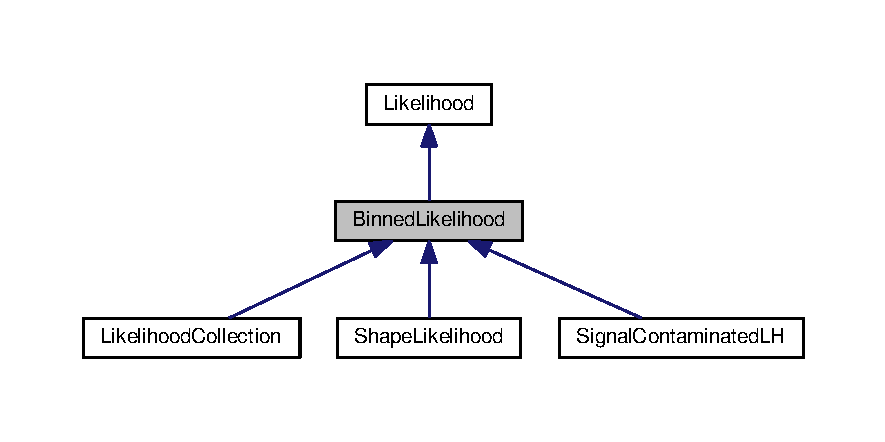
\includegraphics[width=350pt]{classBinnedLikelihood__inherit__graph}
\end{center}
\end{figure}


Collaboration diagram for Binned\-Likelihood\-:
\nopagebreak
\begin{figure}[H]
\begin{center}
\leavevmode
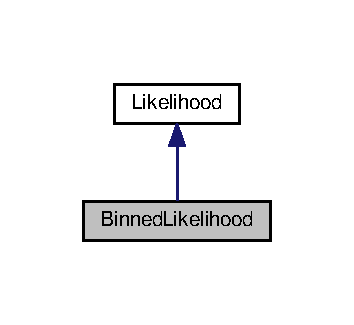
\includegraphics[width=170pt]{classBinnedLikelihood__coll__graph}
\end{center}
\end{figure}
\subsection*{Public Member Functions}
\begin{DoxyCompactItemize}
\item 
\hyperlink{classBinnedLikelihood_acbe8047236d7d3a90f746cdb392eb36f}{Binned\-Likelihood} (int seed, uint64\-\_\-t pdf\-Bins)
\item 
virtual double \hyperlink{classBinnedLikelihood_a2084a64cd8b5d6bf8055538a0f633785}{Evaluate\-L\-L\-H} (double xi) const =0
\item 
double \hyperlink{classBinnedLikelihood_a53d5e07ccbb7b7a5d8c85aeb8f31aa79}{Get\-N\-Total\-L\-L\-H\-Ev} () const 
\begin{DoxyCompactList}\small\item\em Returns the number of likelihood evaluations. \end{DoxyCompactList}\item 
virtual void \hyperlink{classBinnedLikelihood_a0793b8109912c6e509470a14a58d2a2a}{Sample\-Events} (double xi)=0
\begin{DoxyCompactList}\small\item\em Creates internally a new sample with the specified parameter. \end{DoxyCompactList}\item 
virtual \hyperlink{Likelihood_8h_a97d92c5c141f28319e7e8198defc9084}{likelihood\-Callback} \hyperlink{classBinnedLikelihood_aed7e05d58a36f515afc8e34fe8550b31}{Call\-Back\-Fcn} ()=0
\begin{DoxyCompactList}\small\item\em Return the callback function of the likelihood for the minimizer. \end{DoxyCompactList}\item 
virtual double \hyperlink{classBinnedLikelihood_a16f5c7acb008393fcdb12df2524d7033}{Min\-Xi\-Bound} ()
\item 
virtual double \hyperlink{classBinnedLikelihood_ab6144b4d092744dc9d5ee58a491bf77d}{Max\-Xi\-Bound} ()
\item 
void \hyperlink{classBinnedLikelihood_a823016c8e7517bce493f6e3e85559aa9}{Set\-Events} (std\-::vector$<$ uint64\-\_\-t $>$ \&events)
\item 
std\-::vector$<$ uint64\-\_\-t $>$ \& \hyperlink{classBinnedLikelihood_a719edb162d4e030220ebb30374f93eeb}{Get\-Event\-Sample} ()
\item 
uint32\-\_\-t \hyperlink{classBinnedLikelihood_a8b6371a5da5acc90bc1d601422bb9764}{State\-Hash} ()
\begin{DoxyCompactList}\small\item\em Returns a hash number of the observation. \end{DoxyCompactList}\end{DoxyCompactItemize}
\subsection*{Protected Member Functions}
\begin{DoxyCompactItemize}
\item 
void \hyperlink{classBinnedLikelihood_ac72a3e5d0c46e3551f69ea030d4c5ee1}{Histogram\-Events} ()
\end{DoxyCompactItemize}
\subsection*{Protected Attributes}
\begin{DoxyCompactItemize}
\item 
boost\-::shared\-\_\-ptr$<$ \hyperlink{classRNG}{R\-N\-G} $>$ \hyperlink{classBinnedLikelihood_a6a3e39234f7cb8a1a28df28204884632}{rng\-\_\-}
\item 
std\-::vector$<$ uint64\-\_\-t $>$ \hyperlink{classBinnedLikelihood_aa5b023123bb5a1ce1fdd5351ed5e08d2}{observation\-\_\-}
\item 
uint64\-\_\-t \hyperlink{classBinnedLikelihood_af657060cd01071e78f96e272ff3afb2c}{n\-P\-D\-F\-Bins\-\_\-}
\item 
uint64\-\_\-t \hyperlink{classBinnedLikelihood_ad5b5a1f9f9a1db6779f3d82c25b7b0b3}{n\-Total\-L\-L\-H\-Evaluations\-\_\-}
\item 
std\-::vector$<$ uint64\-\_\-t $>$ \hyperlink{classBinnedLikelihood_a4a044760c26d09a93ae8c6a18d44ad88}{used\-Bins\-\_\-}
\end{DoxyCompactItemize}
\subsection*{Additional Inherited Members}


\subsection{Constructor \& Destructor Documentation}
\hypertarget{classBinnedLikelihood_acbe8047236d7d3a90f746cdb392eb36f}{\index{Binned\-Likelihood@{Binned\-Likelihood}!Binned\-Likelihood@{Binned\-Likelihood}}
\index{Binned\-Likelihood@{Binned\-Likelihood}!BinnedLikelihood@{Binned\-Likelihood}}
\subsubsection[{Binned\-Likelihood}]{\setlength{\rightskip}{0pt plus 5cm}Binned\-Likelihood\-::\-Binned\-Likelihood (
\begin{DoxyParamCaption}
\item[{int}]{seed, }
\item[{uint64\-\_\-t}]{pdf\-Bins}
\end{DoxyParamCaption}
)\hspace{0.3cm}{\ttfamily [inline]}}}\label{classBinnedLikelihood_acbe8047236d7d3a90f746cdb392eb36f}


\subsection{Member Function Documentation}
\hypertarget{classBinnedLikelihood_aed7e05d58a36f515afc8e34fe8550b31}{\index{Binned\-Likelihood@{Binned\-Likelihood}!Call\-Back\-Fcn@{Call\-Back\-Fcn}}
\index{Call\-Back\-Fcn@{Call\-Back\-Fcn}!BinnedLikelihood@{Binned\-Likelihood}}
\subsubsection[{Call\-Back\-Fcn}]{\setlength{\rightskip}{0pt plus 5cm}virtual {\bf likelihood\-Callback} Binned\-Likelihood\-::\-Call\-Back\-Fcn (
\begin{DoxyParamCaption}
{}
\end{DoxyParamCaption}
)\hspace{0.3cm}{\ttfamily [pure virtual]}}}\label{classBinnedLikelihood_aed7e05d58a36f515afc8e34fe8550b31}


Return the callback function of the likelihood for the minimizer. 



Implements \hyperlink{classLikelihood_a423872ac038f3fc30d0080f199dc1feb}{Likelihood}.



Implemented in \hyperlink{classShapeLikelihood_acf56e312fd4f0881aa09215d73b93412}{Shape\-Likelihood}, \hyperlink{classLikelihoodCollection_af4c889ced5fc4de6be4ffac2898250b5}{Likelihood\-Collection}, and \hyperlink{classSignalContaminatedLH_a9c67422f6e79df2352bd158be9949feb}{Signal\-Contaminated\-L\-H}.

\hypertarget{classBinnedLikelihood_a2084a64cd8b5d6bf8055538a0f633785}{\index{Binned\-Likelihood@{Binned\-Likelihood}!Evaluate\-L\-L\-H@{Evaluate\-L\-L\-H}}
\index{Evaluate\-L\-L\-H@{Evaluate\-L\-L\-H}!BinnedLikelihood@{Binned\-Likelihood}}
\subsubsection[{Evaluate\-L\-L\-H}]{\setlength{\rightskip}{0pt plus 5cm}virtual double Binned\-Likelihood\-::\-Evaluate\-L\-L\-H (
\begin{DoxyParamCaption}
\item[{double}]{xi}
\end{DoxyParamCaption}
) const\hspace{0.3cm}{\ttfamily [pure virtual]}}}\label{classBinnedLikelihood_a2084a64cd8b5d6bf8055538a0f633785}
Evaluates the log likelihood 
\begin{DoxyParams}{Parameters}
{\em xi} & the likelihood parameter for which the likelihood should be evaulated. \\
\hline
\end{DoxyParams}


Implements \hyperlink{classLikelihood_ab8dd44247a393aa203ff3513b2ba1587}{Likelihood}.



Implemented in \hyperlink{classShapeLikelihood_afe024bedaab4633ded018d23d17c37f8}{Shape\-Likelihood}, \hyperlink{classLikelihoodCollection_a942b79738d2be74a358e138ff5284f53}{Likelihood\-Collection}, and \hyperlink{classSignalContaminatedLH_a30c729fa905cc0d812827f23c71b55cc}{Signal\-Contaminated\-L\-H}.

\hypertarget{classBinnedLikelihood_a719edb162d4e030220ebb30374f93eeb}{\index{Binned\-Likelihood@{Binned\-Likelihood}!Get\-Event\-Sample@{Get\-Event\-Sample}}
\index{Get\-Event\-Sample@{Get\-Event\-Sample}!BinnedLikelihood@{Binned\-Likelihood}}
\subsubsection[{Get\-Event\-Sample}]{\setlength{\rightskip}{0pt plus 5cm}std\-::vector$<$uint64\-\_\-t$>$\& Binned\-Likelihood\-::\-Get\-Event\-Sample (
\begin{DoxyParamCaption}
{}
\end{DoxyParamCaption}
)\hspace{0.3cm}{\ttfamily [inline]}}}\label{classBinnedLikelihood_a719edb162d4e030220ebb30374f93eeb}
\hypertarget{classBinnedLikelihood_a53d5e07ccbb7b7a5d8c85aeb8f31aa79}{\index{Binned\-Likelihood@{Binned\-Likelihood}!Get\-N\-Total\-L\-L\-H\-Ev@{Get\-N\-Total\-L\-L\-H\-Ev}}
\index{Get\-N\-Total\-L\-L\-H\-Ev@{Get\-N\-Total\-L\-L\-H\-Ev}!BinnedLikelihood@{Binned\-Likelihood}}
\subsubsection[{Get\-N\-Total\-L\-L\-H\-Ev}]{\setlength{\rightskip}{0pt plus 5cm}double Binned\-Likelihood\-::\-Get\-N\-Total\-L\-L\-H\-Ev (
\begin{DoxyParamCaption}
{}
\end{DoxyParamCaption}
) const\hspace{0.3cm}{\ttfamily [inline]}}}\label{classBinnedLikelihood_a53d5e07ccbb7b7a5d8c85aeb8f31aa79}


Returns the number of likelihood evaluations. 

\hypertarget{classBinnedLikelihood_ac72a3e5d0c46e3551f69ea030d4c5ee1}{\index{Binned\-Likelihood@{Binned\-Likelihood}!Histogram\-Events@{Histogram\-Events}}
\index{Histogram\-Events@{Histogram\-Events}!BinnedLikelihood@{Binned\-Likelihood}}
\subsubsection[{Histogram\-Events}]{\setlength{\rightskip}{0pt plus 5cm}void Binned\-Likelihood\-::\-Histogram\-Events (
\begin{DoxyParamCaption}
{}
\end{DoxyParamCaption}
)\hspace{0.3cm}{\ttfamily [protected]}}}\label{classBinnedLikelihood_ac72a3e5d0c46e3551f69ea030d4c5ee1}
\hypertarget{classBinnedLikelihood_ab6144b4d092744dc9d5ee58a491bf77d}{\index{Binned\-Likelihood@{Binned\-Likelihood}!Max\-Xi\-Bound@{Max\-Xi\-Bound}}
\index{Max\-Xi\-Bound@{Max\-Xi\-Bound}!BinnedLikelihood@{Binned\-Likelihood}}
\subsubsection[{Max\-Xi\-Bound}]{\setlength{\rightskip}{0pt plus 5cm}virtual double Binned\-Likelihood\-::\-Max\-Xi\-Bound (
\begin{DoxyParamCaption}
{}
\end{DoxyParamCaption}
)\hspace{0.3cm}{\ttfamily [inline]}, {\ttfamily [virtual]}}}\label{classBinnedLikelihood_ab6144b4d092744dc9d5ee58a491bf77d}


Reimplemented from \hyperlink{classLikelihood_a948c31dcc4fe8efc7c39db49ad56c745}{Likelihood}.



Reimplemented in \hyperlink{classLikelihoodCollection_adc81d79fce77d226853f4cfcb33fb7a3}{Likelihood\-Collection}, and \hyperlink{classSignalContaminatedLH_a579d86a266c6ecb44cff26e47d141a9e}{Signal\-Contaminated\-L\-H}.

\hypertarget{classBinnedLikelihood_a16f5c7acb008393fcdb12df2524d7033}{\index{Binned\-Likelihood@{Binned\-Likelihood}!Min\-Xi\-Bound@{Min\-Xi\-Bound}}
\index{Min\-Xi\-Bound@{Min\-Xi\-Bound}!BinnedLikelihood@{Binned\-Likelihood}}
\subsubsection[{Min\-Xi\-Bound}]{\setlength{\rightskip}{0pt plus 5cm}virtual double Binned\-Likelihood\-::\-Min\-Xi\-Bound (
\begin{DoxyParamCaption}
{}
\end{DoxyParamCaption}
)\hspace{0.3cm}{\ttfamily [inline]}, {\ttfamily [virtual]}}}\label{classBinnedLikelihood_a16f5c7acb008393fcdb12df2524d7033}


Reimplemented from \hyperlink{classLikelihood_a5af640d09a81f553b8331d2557b01aa6}{Likelihood}.

\hypertarget{classBinnedLikelihood_a0793b8109912c6e509470a14a58d2a2a}{\index{Binned\-Likelihood@{Binned\-Likelihood}!Sample\-Events@{Sample\-Events}}
\index{Sample\-Events@{Sample\-Events}!BinnedLikelihood@{Binned\-Likelihood}}
\subsubsection[{Sample\-Events}]{\setlength{\rightskip}{0pt plus 5cm}virtual void Binned\-Likelihood\-::\-Sample\-Events (
\begin{DoxyParamCaption}
\item[{double}]{xi}
\end{DoxyParamCaption}
)\hspace{0.3cm}{\ttfamily [pure virtual]}}}\label{classBinnedLikelihood_a0793b8109912c6e509470a14a58d2a2a}


Creates internally a new sample with the specified parameter. 



Implements \hyperlink{classLikelihood_a11245b8594fa8658698798d92a56e4d8}{Likelihood}.



Implemented in \hyperlink{classShapeLikelihood_aa303861500c399cb680d89b15d08b806}{Shape\-Likelihood}, \hyperlink{classLikelihoodCollection_a38af4d60e248c8d32d0b05ce623c031b}{Likelihood\-Collection}, and \hyperlink{classSignalContaminatedLH_a04fcf69547f8b0c5bc3ee2cb89671c06}{Signal\-Contaminated\-L\-H}.

\hypertarget{classBinnedLikelihood_a823016c8e7517bce493f6e3e85559aa9}{\index{Binned\-Likelihood@{Binned\-Likelihood}!Set\-Events@{Set\-Events}}
\index{Set\-Events@{Set\-Events}!BinnedLikelihood@{Binned\-Likelihood}}
\subsubsection[{Set\-Events}]{\setlength{\rightskip}{0pt plus 5cm}void Binned\-Likelihood\-::\-Set\-Events (
\begin{DoxyParamCaption}
\item[{std\-::vector$<$ uint64\-\_\-t $>$ \&}]{events}
\end{DoxyParamCaption}
)\hspace{0.3cm}{\ttfamily [inline]}}}\label{classBinnedLikelihood_a823016c8e7517bce493f6e3e85559aa9}
This function is used to set the event sample for the likelihood to be computed. 
\begin{DoxyParams}{Parameters}
{\em events} & a vector containing the binned event sample that the analysis should run on. \\
\hline
\end{DoxyParams}
\hypertarget{classBinnedLikelihood_a8b6371a5da5acc90bc1d601422bb9764}{\index{Binned\-Likelihood@{Binned\-Likelihood}!State\-Hash@{State\-Hash}}
\index{State\-Hash@{State\-Hash}!BinnedLikelihood@{Binned\-Likelihood}}
\subsubsection[{State\-Hash}]{\setlength{\rightskip}{0pt plus 5cm}uint32\-\_\-t Binned\-Likelihood\-::\-State\-Hash (
\begin{DoxyParamCaption}
{}
\end{DoxyParamCaption}
)\hspace{0.3cm}{\ttfamily [inline]}, {\ttfamily [virtual]}}}\label{classBinnedLikelihood_a8b6371a5da5acc90bc1d601422bb9764}


Returns a hash number of the observation. 



Implements \hyperlink{classLikelihood_a5e38ffabbfeba8196b71073effc497c9}{Likelihood}.



\subsection{Member Data Documentation}
\hypertarget{classBinnedLikelihood_af657060cd01071e78f96e272ff3afb2c}{\index{Binned\-Likelihood@{Binned\-Likelihood}!n\-P\-D\-F\-Bins\-\_\-@{n\-P\-D\-F\-Bins\-\_\-}}
\index{n\-P\-D\-F\-Bins\-\_\-@{n\-P\-D\-F\-Bins\-\_\-}!BinnedLikelihood@{Binned\-Likelihood}}
\subsubsection[{n\-P\-D\-F\-Bins\-\_\-}]{\setlength{\rightskip}{0pt plus 5cm}uint64\-\_\-t Binned\-Likelihood\-::n\-P\-D\-F\-Bins\-\_\-\hspace{0.3cm}{\ttfamily [protected]}}}\label{classBinnedLikelihood_af657060cd01071e78f96e272ff3afb2c}
\hypertarget{classBinnedLikelihood_ad5b5a1f9f9a1db6779f3d82c25b7b0b3}{\index{Binned\-Likelihood@{Binned\-Likelihood}!n\-Total\-L\-L\-H\-Evaluations\-\_\-@{n\-Total\-L\-L\-H\-Evaluations\-\_\-}}
\index{n\-Total\-L\-L\-H\-Evaluations\-\_\-@{n\-Total\-L\-L\-H\-Evaluations\-\_\-}!BinnedLikelihood@{Binned\-Likelihood}}
\subsubsection[{n\-Total\-L\-L\-H\-Evaluations\-\_\-}]{\setlength{\rightskip}{0pt plus 5cm}uint64\-\_\-t Binned\-Likelihood\-::n\-Total\-L\-L\-H\-Evaluations\-\_\-\hspace{0.3cm}{\ttfamily [mutable]}, {\ttfamily [protected]}}}\label{classBinnedLikelihood_ad5b5a1f9f9a1db6779f3d82c25b7b0b3}
\hypertarget{classBinnedLikelihood_aa5b023123bb5a1ce1fdd5351ed5e08d2}{\index{Binned\-Likelihood@{Binned\-Likelihood}!observation\-\_\-@{observation\-\_\-}}
\index{observation\-\_\-@{observation\-\_\-}!BinnedLikelihood@{Binned\-Likelihood}}
\subsubsection[{observation\-\_\-}]{\setlength{\rightskip}{0pt plus 5cm}std\-::vector$<$uint64\-\_\-t$>$ Binned\-Likelihood\-::observation\-\_\-\hspace{0.3cm}{\ttfamily [protected]}}}\label{classBinnedLikelihood_aa5b023123bb5a1ce1fdd5351ed5e08d2}
\hypertarget{classBinnedLikelihood_a6a3e39234f7cb8a1a28df28204884632}{\index{Binned\-Likelihood@{Binned\-Likelihood}!rng\-\_\-@{rng\-\_\-}}
\index{rng\-\_\-@{rng\-\_\-}!BinnedLikelihood@{Binned\-Likelihood}}
\subsubsection[{rng\-\_\-}]{\setlength{\rightskip}{0pt plus 5cm}boost\-::shared\-\_\-ptr$<${\bf R\-N\-G}$>$ Binned\-Likelihood\-::rng\-\_\-\hspace{0.3cm}{\ttfamily [protected]}}}\label{classBinnedLikelihood_a6a3e39234f7cb8a1a28df28204884632}
\hypertarget{classBinnedLikelihood_a4a044760c26d09a93ae8c6a18d44ad88}{\index{Binned\-Likelihood@{Binned\-Likelihood}!used\-Bins\-\_\-@{used\-Bins\-\_\-}}
\index{used\-Bins\-\_\-@{used\-Bins\-\_\-}!BinnedLikelihood@{Binned\-Likelihood}}
\subsubsection[{used\-Bins\-\_\-}]{\setlength{\rightskip}{0pt plus 5cm}std\-::vector$<$uint64\-\_\-t$>$ Binned\-Likelihood\-::used\-Bins\-\_\-\hspace{0.3cm}{\ttfamily [protected]}}}\label{classBinnedLikelihood_a4a044760c26d09a93ae8c6a18d44ad88}


The documentation for this class was generated from the following file\-:\begin{DoxyCompactItemize}
\item 
/home/travis/build/sflis/\-M\-L\-Sandbox/public/\-M\-L\-Sandbox/\hyperlink{Likelihood_8h}{Likelihood.\-h}\end{DoxyCompactItemize}

\hypertarget{classCombinedLikelihood}{\section{Combined\-Likelihood Class Reference}
\label{classCombinedLikelihood}\index{Combined\-Likelihood@{Combined\-Likelihood}}
}


{\ttfamily \#include $<$Combined\-Likelihood.\-h$>$}



Inheritance diagram for Combined\-Likelihood\-:
\nopagebreak
\begin{figure}[H]
\begin{center}
\leavevmode
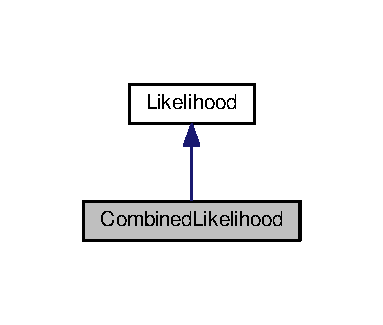
\includegraphics[width=184pt]{classCombinedLikelihood__inherit__graph}
\end{center}
\end{figure}


Collaboration diagram for Combined\-Likelihood\-:
\nopagebreak
\begin{figure}[H]
\begin{center}
\leavevmode
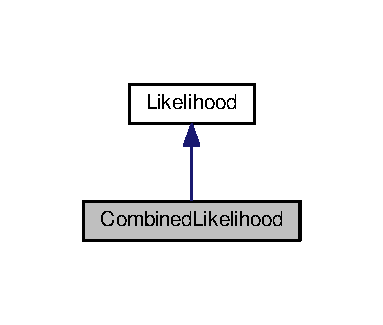
\includegraphics[width=184pt]{classCombinedLikelihood__coll__graph}
\end{center}
\end{figure}
\subsection*{Public Member Functions}
\begin{DoxyCompactItemize}
\item 
\hyperlink{classCombinedLikelihood_a5f4928ccb337b399d64088e3df58d7be}{Combined\-Likelihood} (const std\-::vector$<$ boost\-::shared\-\_\-ptr$<$ \hyperlink{classLikelihood}{Likelihood} $>$ $>$ \&likelihoods\-\_\-, const std\-::vector$<$ double $>$ \&weights\-\_\-)
\item 
double \hyperlink{classCombinedLikelihood_a5d41f29fd87fcab976a06e0af12e6767}{Evaluate\-L\-L\-H} (double xi) const 
\item 
void \hyperlink{classCombinedLikelihood_a2e3dc150595fdab805b77fc8f2557fa0}{Sample\-Events} (double xi)
\item 
\hyperlink{Likelihood_8h_a97d92c5c141f28319e7e8198defc9084}{likelihood\-Callback} \hyperlink{classCombinedLikelihood_a4d70d16e3f63005427dc9261addd0bfb}{Call\-Back\-Fcn} ()
\item 
\hyperlink{classCombinedLikelihood}{Combined\-Likelihood} $\ast$ \hyperlink{classCombinedLikelihood_afb2505b9b126ddfcc859b150e8345aed}{Clone} (int seed) const 
\item 
uint32\-\_\-t \hyperlink{classCombinedLikelihood_a7980d2517a55eea72e7e272917b1948d}{State\-Hash} ()
\begin{DoxyCompactList}\small\item\em Returns a hash number of the observation. \end{DoxyCompactList}\item 
double \hyperlink{classCombinedLikelihood_a2cf396d545d7873be85a9bbcb72f4b53}{Max\-Xi\-Bound} ()
\item 
void \hyperlink{classCombinedLikelihood_ae6823517190d050b153d421c46a6cd0f}{Update} ()
\end{DoxyCompactItemize}
\subsection*{Additional Inherited Members}


\subsection{Constructor \& Destructor Documentation}
\hypertarget{classCombinedLikelihood_a5f4928ccb337b399d64088e3df58d7be}{\index{Combined\-Likelihood@{Combined\-Likelihood}!Combined\-Likelihood@{Combined\-Likelihood}}
\index{Combined\-Likelihood@{Combined\-Likelihood}!CombinedLikelihood@{Combined\-Likelihood}}
\subsubsection[{Combined\-Likelihood}]{\setlength{\rightskip}{0pt plus 5cm}Combined\-Likelihood\-::\-Combined\-Likelihood (
\begin{DoxyParamCaption}
\item[{const std\-::vector$<$ boost\-::shared\-\_\-ptr$<$ {\bf Likelihood} $>$ $>$ \&}]{likelihoods\-\_\-, }
\item[{const std\-::vector$<$ double $>$ \&}]{weights\-\_\-}
\end{DoxyParamCaption}
)\hspace{0.3cm}{\ttfamily [inline]}}}\label{classCombinedLikelihood_a5f4928ccb337b399d64088e3df58d7be}


\subsection{Member Function Documentation}
\hypertarget{classCombinedLikelihood_a4d70d16e3f63005427dc9261addd0bfb}{\index{Combined\-Likelihood@{Combined\-Likelihood}!Call\-Back\-Fcn@{Call\-Back\-Fcn}}
\index{Call\-Back\-Fcn@{Call\-Back\-Fcn}!CombinedLikelihood@{Combined\-Likelihood}}
\subsubsection[{Call\-Back\-Fcn}]{\setlength{\rightskip}{0pt plus 5cm}{\bf likelihood\-Callback} Combined\-Likelihood\-::\-Call\-Back\-Fcn (
\begin{DoxyParamCaption}
{}
\end{DoxyParamCaption}
)\hspace{0.3cm}{\ttfamily [inline]}, {\ttfamily [virtual]}}}\label{classCombinedLikelihood_a4d70d16e3f63005427dc9261addd0bfb}
Return the callback function of the likelihood for the minimizer \begin{DoxyReturn}{Returns}
A function pointer function of the type double(double,void$\ast$) 
\end{DoxyReturn}


Implements \hyperlink{classLikelihood_a423872ac038f3fc30d0080f199dc1feb}{Likelihood}.

\hypertarget{classCombinedLikelihood_afb2505b9b126ddfcc859b150e8345aed}{\index{Combined\-Likelihood@{Combined\-Likelihood}!Clone@{Clone}}
\index{Clone@{Clone}!CombinedLikelihood@{Combined\-Likelihood}}
\subsubsection[{Clone}]{\setlength{\rightskip}{0pt plus 5cm}{\bf Combined\-Likelihood}$\ast$ Combined\-Likelihood\-::\-Clone (
\begin{DoxyParamCaption}
\item[{int}]{seed}
\end{DoxyParamCaption}
) const\hspace{0.3cm}{\ttfamily [inline]}, {\ttfamily [virtual]}}}\label{classCombinedLikelihood_afb2505b9b126ddfcc859b150e8345aed}
Should create a copy of the original \hyperlink{classLikelihood}{Likelihood} which is thread safe. 

Implements \hyperlink{classLikelihood_a938b362a171c46f447cb364effc83bcf}{Likelihood}.

\hypertarget{classCombinedLikelihood_a5d41f29fd87fcab976a06e0af12e6767}{\index{Combined\-Likelihood@{Combined\-Likelihood}!Evaluate\-L\-L\-H@{Evaluate\-L\-L\-H}}
\index{Evaluate\-L\-L\-H@{Evaluate\-L\-L\-H}!CombinedLikelihood@{Combined\-Likelihood}}
\subsubsection[{Evaluate\-L\-L\-H}]{\setlength{\rightskip}{0pt plus 5cm}double Combined\-Likelihood\-::\-Evaluate\-L\-L\-H (
\begin{DoxyParamCaption}
\item[{double}]{xi}
\end{DoxyParamCaption}
) const\hspace{0.3cm}{\ttfamily [virtual]}}}\label{classCombinedLikelihood_a5d41f29fd87fcab976a06e0af12e6767}
Evaluates the log likelihood sum 
\begin{DoxyParams}{Parameters}
{\em xi} & the signal fraction for which the likelihood should be evaulated. \\
\hline
\end{DoxyParams}


Implements \hyperlink{classLikelihood_ab8dd44247a393aa203ff3513b2ba1587}{Likelihood}.

\hypertarget{classCombinedLikelihood_a2cf396d545d7873be85a9bbcb72f4b53}{\index{Combined\-Likelihood@{Combined\-Likelihood}!Max\-Xi\-Bound@{Max\-Xi\-Bound}}
\index{Max\-Xi\-Bound@{Max\-Xi\-Bound}!CombinedLikelihood@{Combined\-Likelihood}}
\subsubsection[{Max\-Xi\-Bound}]{\setlength{\rightskip}{0pt plus 5cm}double Combined\-Likelihood\-::\-Max\-Xi\-Bound (
\begin{DoxyParamCaption}
{}
\end{DoxyParamCaption}
)\hspace{0.3cm}{\ttfamily [virtual]}}}\label{classCombinedLikelihood_a2cf396d545d7873be85a9bbcb72f4b53}


Reimplemented from \hyperlink{classLikelihood_a948c31dcc4fe8efc7c39db49ad56c745}{Likelihood}.

\hypertarget{classCombinedLikelihood_a2e3dc150595fdab805b77fc8f2557fa0}{\index{Combined\-Likelihood@{Combined\-Likelihood}!Sample\-Events@{Sample\-Events}}
\index{Sample\-Events@{Sample\-Events}!CombinedLikelihood@{Combined\-Likelihood}}
\subsubsection[{Sample\-Events}]{\setlength{\rightskip}{0pt plus 5cm}void Combined\-Likelihood\-::\-Sample\-Events (
\begin{DoxyParamCaption}
\item[{double}]{xi}
\end{DoxyParamCaption}
)\hspace{0.3cm}{\ttfamily [virtual]}}}\label{classCombinedLikelihood_a2e3dc150595fdab805b77fc8f2557fa0}
Creates internally a new sample with the specified parameter likelihood parameter 
\begin{DoxyParams}{Parameters}
{\em xi} & value of the likelihood parameter \\
\hline
\end{DoxyParams}


Implements \hyperlink{classLikelihood_a11245b8594fa8658698798d92a56e4d8}{Likelihood}.

\hypertarget{classCombinedLikelihood_a7980d2517a55eea72e7e272917b1948d}{\index{Combined\-Likelihood@{Combined\-Likelihood}!State\-Hash@{State\-Hash}}
\index{State\-Hash@{State\-Hash}!CombinedLikelihood@{Combined\-Likelihood}}
\subsubsection[{State\-Hash}]{\setlength{\rightskip}{0pt plus 5cm}uint32\-\_\-t Combined\-Likelihood\-::\-State\-Hash (
\begin{DoxyParamCaption}
{}
\end{DoxyParamCaption}
)\hspace{0.3cm}{\ttfamily [inline]}, {\ttfamily [virtual]}}}\label{classCombinedLikelihood_a7980d2517a55eea72e7e272917b1948d}


Returns a hash number of the observation. 



Implements \hyperlink{classLikelihood_a5e38ffabbfeba8196b71073effc497c9}{Likelihood}.

\hypertarget{classCombinedLikelihood_ae6823517190d050b153d421c46a6cd0f}{\index{Combined\-Likelihood@{Combined\-Likelihood}!Update@{Update}}
\index{Update@{Update}!CombinedLikelihood@{Combined\-Likelihood}}
\subsubsection[{Update}]{\setlength{\rightskip}{0pt plus 5cm}void Combined\-Likelihood\-::\-Update (
\begin{DoxyParamCaption}
{}
\end{DoxyParamCaption}
)\hspace{0.3cm}{\ttfamily [inline]}}}\label{classCombinedLikelihood_ae6823517190d050b153d421c46a6cd0f}


The documentation for this class was generated from the following files\-:\begin{DoxyCompactItemize}
\item 
/home/travis/build/sflis/\-M\-L\-Sandbox/public/\-M\-L\-Sandbox/\hyperlink{CombinedLikelihood_8h}{Combined\-Likelihood.\-h}\item 
/home/travis/build/sflis/\-M\-L\-Sandbox/private/\-M\-L\-Sandbox/\hyperlink{CombinedLikelihood_8cxx}{Combined\-Likelihood.\-cxx}\end{DoxyCompactItemize}

\hypertarget{classDistribution}{\section{Distribution Class Reference}
\label{classDistribution}\index{Distribution@{Distribution}}
}


A class that provides a common interface for binned distributions which are used to represent binned pdfs in likelihood objects.  




{\ttfamily \#include $<$Distribution.\-h$>$}

\subsection*{Public Member Functions}
\begin{DoxyCompactItemize}
\item 
\hyperlink{classDistribution_a7671d190019f4e6d1014a561a9e3cc65}{Distribution} (\hyperlink{classDistribution}{Distribution} const \&base, boost\-::shared\-\_\-ptr$<$ \hyperlink{classRNG}{R\-N\-G} $>$ rng)
\item 
\hyperlink{classDistribution_a2ee6e69ceb1df2813df56c6883cbb326}{Distribution} (std\-::vector$<$ double $>$const \&distribution, double r\-Min, double r\-Max, uint r\-Seed=1)
\item 
double \hyperlink{classDistribution_a26a55e9b524f94fb5c75e3c8abe96ecd}{P\-D\-F} (double x) const 
\begin{DoxyCompactList}\small\item\em Returns the pdf value evaluated at the given value. \end{DoxyCompactList}\item 
double \hyperlink{classDistribution_a94a970330e540c2061d6c05dc9f60f1d}{P\-D\-F\-\_\-f} (double x) const 
\item 
double \hyperlink{classDistribution_ac852b7915ba69e2d8f9cee0e5dab68b5}{C\-D\-F} (double x) const 
\begin{DoxyCompactList}\small\item\em Evaluates the C\-D\-F at a given value. \end{DoxyCompactList}\item 
double \hyperlink{classDistribution_a503ae8b2d80c3c26a8c9a255c59761f2}{Sample\-From\-Distr} () const 
\begin{DoxyCompactList}\small\item\em Returns a random number sampled according to the binned distribution. \end{DoxyCompactList}\item 
uint64\-\_\-t \hyperlink{classDistribution_aeaaf3037d0c8167d4c41fe4213df3181}{Sample\-From\-Distr\-I} () const 
\begin{DoxyCompactList}\small\item\em Returns a random index of the binned distribution sampled according to the same distribution. \end{DoxyCompactList}\item 
uint64\-\_\-t \hyperlink{classDistribution_a8d5beb423a42b4acb0724e24ddb05195}{Get\-N\-Bins} () const 
\begin{DoxyCompactList}\small\item\em Returns the number of bins of the pdf. \end{DoxyCompactList}\item 
uint64\-\_\-t \hyperlink{classDistribution_a14d717bbe93f876772eead67bd413f2b}{Value\-To\-Bin} (double x)
\begin{DoxyCompactList}\small\item\em Returns the bin index of the binned pdf corresponding to the givem value. \end{DoxyCompactList}\item 
std\-::vector$<$ double $>$ \& \hyperlink{classDistribution_a58298747fcca2bd64976ae247df3f3e5}{Get\-P\-D\-F\-Vector} ()
\begin{DoxyCompactList}\small\item\em Returns a reference to the pdf. \end{DoxyCompactList}\item 
double \hyperlink{classDistribution_a52415dcd5a27eb454df64912597eb95a}{operator\mbox{[}$\,$\mbox{]}} (uint64\-\_\-t index)
\begin{DoxyCompactList}\small\item\em Provides direct access to the binned pdf. \end{DoxyCompactList}\item 
double \hyperlink{classDistribution_a7e969b8ea60baa6498ca6951b205f967}{operator\mbox{[}$\,$\mbox{]}} (uint64\-\_\-t index) const 
\begin{DoxyCompactList}\small\item\em Provides direct access to the binned pdf (const) \end{DoxyCompactList}\item 
void \hyperlink{classDistribution_a9cc42751d710907d76d97813b8fa8697}{Set\-C\-D\-F\-Sampling} (bool set)
\item 
double \hyperlink{classDistribution_a3802925dff4de220fbe8e214e42e1e33}{Get\-Range\-Max} () const 
\item 
double \hyperlink{classDistribution_a10e8b59653c735c0dceae1d3c15b2713}{Get\-Range\-Min} () const 
\end{DoxyCompactItemize}
\subsection*{Friends}
\begin{DoxyCompactItemize}
\item 
void \hyperlink{classDistribution_ab7b6b8c6018ab181645199038b0dba3a}{add\-Distributions} (double w1, \hyperlink{classDistribution}{Distribution} const \&dst1, double w2, \hyperlink{classDistribution}{Distribution} const \&dst2, \hyperlink{classDistribution}{Distribution} \&target)
\end{DoxyCompactItemize}


\subsection{Detailed Description}
A class that provides a common interface for binned distributions which are used to represent binned pdfs in likelihood objects. 

class\-: \hyperlink{classDistribution}{Distribution} 

\subsection{Constructor \& Destructor Documentation}
\hypertarget{classDistribution_a7671d190019f4e6d1014a561a9e3cc65}{\index{Distribution@{Distribution}!Distribution@{Distribution}}
\index{Distribution@{Distribution}!Distribution@{Distribution}}
\subsubsection[{Distribution}]{\setlength{\rightskip}{0pt plus 5cm}Distribution\-::\-Distribution (
\begin{DoxyParamCaption}
\item[{{\bf Distribution} const \&}]{base, }
\item[{boost\-::shared\-\_\-ptr$<$ {\bf R\-N\-G} $>$}]{rng}
\end{DoxyParamCaption}
)}}\label{classDistribution_a7671d190019f4e6d1014a561a9e3cc65}
\hypertarget{classDistribution_a2ee6e69ceb1df2813df56c6883cbb326}{\index{Distribution@{Distribution}!Distribution@{Distribution}}
\index{Distribution@{Distribution}!Distribution@{Distribution}}
\subsubsection[{Distribution}]{\setlength{\rightskip}{0pt plus 5cm}Distribution\-::\-Distribution (
\begin{DoxyParamCaption}
\item[{std\-::vector$<$ double $>$const \&}]{distribution, }
\item[{double}]{r\-Min, }
\item[{double}]{r\-Max, }
\item[{uint}]{r\-Seed = {\ttfamily 1}}
\end{DoxyParamCaption}
)}}\label{classDistribution_a2ee6e69ceb1df2813df56c6883cbb326}


\subsection{Member Function Documentation}
\hypertarget{classDistribution_ac852b7915ba69e2d8f9cee0e5dab68b5}{\index{Distribution@{Distribution}!C\-D\-F@{C\-D\-F}}
\index{C\-D\-F@{C\-D\-F}!Distribution@{Distribution}}
\subsubsection[{C\-D\-F}]{\setlength{\rightskip}{0pt plus 5cm}double Distribution\-::\-C\-D\-F (
\begin{DoxyParamCaption}
\item[{double}]{x}
\end{DoxyParamCaption}
) const}}\label{classDistribution_ac852b7915ba69e2d8f9cee0e5dab68b5}


Evaluates the C\-D\-F at a given value. 

\hypertarget{classDistribution_a8d5beb423a42b4acb0724e24ddb05195}{\index{Distribution@{Distribution}!Get\-N\-Bins@{Get\-N\-Bins}}
\index{Get\-N\-Bins@{Get\-N\-Bins}!Distribution@{Distribution}}
\subsubsection[{Get\-N\-Bins}]{\setlength{\rightskip}{0pt plus 5cm}uint64\-\_\-t Distribution\-::\-Get\-N\-Bins (
\begin{DoxyParamCaption}
{}
\end{DoxyParamCaption}
) const\hspace{0.3cm}{\ttfamily [inline]}}}\label{classDistribution_a8d5beb423a42b4acb0724e24ddb05195}


Returns the number of bins of the pdf. 

\hypertarget{classDistribution_a58298747fcca2bd64976ae247df3f3e5}{\index{Distribution@{Distribution}!Get\-P\-D\-F\-Vector@{Get\-P\-D\-F\-Vector}}
\index{Get\-P\-D\-F\-Vector@{Get\-P\-D\-F\-Vector}!Distribution@{Distribution}}
\subsubsection[{Get\-P\-D\-F\-Vector}]{\setlength{\rightskip}{0pt plus 5cm}std\-::vector$<$double$>$\& Distribution\-::\-Get\-P\-D\-F\-Vector (
\begin{DoxyParamCaption}
{}
\end{DoxyParamCaption}
)\hspace{0.3cm}{\ttfamily [inline]}}}\label{classDistribution_a58298747fcca2bd64976ae247df3f3e5}


Returns a reference to the pdf. 

\hypertarget{classDistribution_a3802925dff4de220fbe8e214e42e1e33}{\index{Distribution@{Distribution}!Get\-Range\-Max@{Get\-Range\-Max}}
\index{Get\-Range\-Max@{Get\-Range\-Max}!Distribution@{Distribution}}
\subsubsection[{Get\-Range\-Max}]{\setlength{\rightskip}{0pt plus 5cm}double Distribution\-::\-Get\-Range\-Max (
\begin{DoxyParamCaption}
{}
\end{DoxyParamCaption}
) const\hspace{0.3cm}{\ttfamily [inline]}}}\label{classDistribution_a3802925dff4de220fbe8e214e42e1e33}
\hypertarget{classDistribution_a10e8b59653c735c0dceae1d3c15b2713}{\index{Distribution@{Distribution}!Get\-Range\-Min@{Get\-Range\-Min}}
\index{Get\-Range\-Min@{Get\-Range\-Min}!Distribution@{Distribution}}
\subsubsection[{Get\-Range\-Min}]{\setlength{\rightskip}{0pt plus 5cm}double Distribution\-::\-Get\-Range\-Min (
\begin{DoxyParamCaption}
{}
\end{DoxyParamCaption}
) const\hspace{0.3cm}{\ttfamily [inline]}}}\label{classDistribution_a10e8b59653c735c0dceae1d3c15b2713}
\hypertarget{classDistribution_a52415dcd5a27eb454df64912597eb95a}{\index{Distribution@{Distribution}!operator\mbox{[}$\,$\mbox{]}@{operator[]}}
\index{operator\mbox{[}$\,$\mbox{]}@{operator[]}!Distribution@{Distribution}}
\subsubsection[{operator[]}]{\setlength{\rightskip}{0pt plus 5cm}double Distribution\-::operator\mbox{[}$\,$\mbox{]} (
\begin{DoxyParamCaption}
\item[{uint64\-\_\-t}]{index}
\end{DoxyParamCaption}
)\hspace{0.3cm}{\ttfamily [inline]}}}\label{classDistribution_a52415dcd5a27eb454df64912597eb95a}


Provides direct access to the binned pdf. 

\hypertarget{classDistribution_a7e969b8ea60baa6498ca6951b205f967}{\index{Distribution@{Distribution}!operator\mbox{[}$\,$\mbox{]}@{operator[]}}
\index{operator\mbox{[}$\,$\mbox{]}@{operator[]}!Distribution@{Distribution}}
\subsubsection[{operator[]}]{\setlength{\rightskip}{0pt plus 5cm}double Distribution\-::operator\mbox{[}$\,$\mbox{]} (
\begin{DoxyParamCaption}
\item[{uint64\-\_\-t}]{index}
\end{DoxyParamCaption}
) const\hspace{0.3cm}{\ttfamily [inline]}}}\label{classDistribution_a7e969b8ea60baa6498ca6951b205f967}


Provides direct access to the binned pdf (const) 

\hypertarget{classDistribution_a26a55e9b524f94fb5c75e3c8abe96ecd}{\index{Distribution@{Distribution}!P\-D\-F@{P\-D\-F}}
\index{P\-D\-F@{P\-D\-F}!Distribution@{Distribution}}
\subsubsection[{P\-D\-F}]{\setlength{\rightskip}{0pt plus 5cm}double Distribution\-::\-P\-D\-F (
\begin{DoxyParamCaption}
\item[{double}]{x}
\end{DoxyParamCaption}
) const}}\label{classDistribution_a26a55e9b524f94fb5c75e3c8abe96ecd}


Returns the pdf value evaluated at the given value. 

\hypertarget{classDistribution_a94a970330e540c2061d6c05dc9f60f1d}{\index{Distribution@{Distribution}!P\-D\-F\-\_\-f@{P\-D\-F\-\_\-f}}
\index{P\-D\-F\-\_\-f@{P\-D\-F\-\_\-f}!Distribution@{Distribution}}
\subsubsection[{P\-D\-F\-\_\-f}]{\setlength{\rightskip}{0pt plus 5cm}double Distribution\-::\-P\-D\-F\-\_\-f (
\begin{DoxyParamCaption}
\item[{double}]{x}
\end{DoxyParamCaption}
) const\hspace{0.3cm}{\ttfamily [inline]}}}\label{classDistribution_a94a970330e540c2061d6c05dc9f60f1d}
Fast unsafe call to P\-D\-F (no boundary checks) 
\begin{DoxyParams}{Parameters}
{\em x} & the pdf paramater at which the pdf should be evaluated at \\
\hline
\end{DoxyParams}
\begin{DoxyReturn}{Returns}
pdf value at x 
\end{DoxyReturn}
\hypertarget{classDistribution_a503ae8b2d80c3c26a8c9a255c59761f2}{\index{Distribution@{Distribution}!Sample\-From\-Distr@{Sample\-From\-Distr}}
\index{Sample\-From\-Distr@{Sample\-From\-Distr}!Distribution@{Distribution}}
\subsubsection[{Sample\-From\-Distr}]{\setlength{\rightskip}{0pt plus 5cm}double Distribution\-::\-Sample\-From\-Distr (
\begin{DoxyParamCaption}
{}
\end{DoxyParamCaption}
) const}}\label{classDistribution_a503ae8b2d80c3c26a8c9a255c59761f2}


Returns a random number sampled according to the binned distribution. 

\hypertarget{classDistribution_aeaaf3037d0c8167d4c41fe4213df3181}{\index{Distribution@{Distribution}!Sample\-From\-Distr\-I@{Sample\-From\-Distr\-I}}
\index{Sample\-From\-Distr\-I@{Sample\-From\-Distr\-I}!Distribution@{Distribution}}
\subsubsection[{Sample\-From\-Distr\-I}]{\setlength{\rightskip}{0pt plus 5cm}uint64\-\_\-t Distribution\-::\-Sample\-From\-Distr\-I (
\begin{DoxyParamCaption}
{}
\end{DoxyParamCaption}
) const\hspace{0.3cm}{\ttfamily [inline]}}}\label{classDistribution_aeaaf3037d0c8167d4c41fe4213df3181}


Returns a random index of the binned distribution sampled according to the same distribution. 

\hypertarget{classDistribution_a9cc42751d710907d76d97813b8fa8697}{\index{Distribution@{Distribution}!Set\-C\-D\-F\-Sampling@{Set\-C\-D\-F\-Sampling}}
\index{Set\-C\-D\-F\-Sampling@{Set\-C\-D\-F\-Sampling}!Distribution@{Distribution}}
\subsubsection[{Set\-C\-D\-F\-Sampling}]{\setlength{\rightskip}{0pt plus 5cm}void Distribution\-::\-Set\-C\-D\-F\-Sampling (
\begin{DoxyParamCaption}
\item[{bool}]{set}
\end{DoxyParamCaption}
)\hspace{0.3cm}{\ttfamily [inline]}}}\label{classDistribution_a9cc42751d710907d76d97813b8fa8697}
\hypertarget{classDistribution_a14d717bbe93f876772eead67bd413f2b}{\index{Distribution@{Distribution}!Value\-To\-Bin@{Value\-To\-Bin}}
\index{Value\-To\-Bin@{Value\-To\-Bin}!Distribution@{Distribution}}
\subsubsection[{Value\-To\-Bin}]{\setlength{\rightskip}{0pt plus 5cm}uint64\-\_\-t Distribution\-::\-Value\-To\-Bin (
\begin{DoxyParamCaption}
\item[{double}]{x}
\end{DoxyParamCaption}
)\hspace{0.3cm}{\ttfamily [inline]}}}\label{classDistribution_a14d717bbe93f876772eead67bd413f2b}


Returns the bin index of the binned pdf corresponding to the givem value. 



\subsection{Friends And Related Function Documentation}
\hypertarget{classDistribution_ab7b6b8c6018ab181645199038b0dba3a}{\index{Distribution@{Distribution}!add\-Distributions@{add\-Distributions}}
\index{add\-Distributions@{add\-Distributions}!Distribution@{Distribution}}
\subsubsection[{add\-Distributions}]{\setlength{\rightskip}{0pt plus 5cm}void add\-Distributions (
\begin{DoxyParamCaption}
\item[{double}]{w1, }
\item[{{\bf Distribution} const \&}]{dst1, }
\item[{double}]{w2, }
\item[{{\bf Distribution} const \&}]{dst2, }
\item[{{\bf Distribution} \&}]{target}
\end{DoxyParamCaption}
)\hspace{0.3cm}{\ttfamily [friend]}}}\label{classDistribution_ab7b6b8c6018ab181645199038b0dba3a}
A helper function that performs an addition operation on two distributions and putting the result in a third distribution object 

The documentation for this class was generated from the following files\-:\begin{DoxyCompactItemize}
\item 
/home/travis/build/sflis/\-M\-L\-Sandbox/public/\-M\-L\-Sandbox/\hyperlink{Distribution_8h}{Distribution.\-h}\item 
/home/travis/build/sflis/\-M\-L\-Sandbox/private/\-M\-L\-Sandbox/\hyperlink{MLSandbox_2Distribution_8cxx}{Distribution.\-cxx}\end{DoxyCompactItemize}

\hypertarget{classFCRanks}{\section{F\-C\-Ranks Class Reference}
\label{classFCRanks}\index{F\-C\-Ranks@{F\-C\-Ranks}}
}


A class that holds Feldman Cousins rank distribtions and provides some utilities to interpolate the critical boundary at different confidence levels.  




{\ttfamily \#include $<$F\-C\-Ranks.\-h$>$}

\subsection*{Public Member Functions}
\begin{DoxyCompactItemize}
\item 
\hyperlink{classFCRanks_a6db5a79e4fc52467381a44faaf6df285}{F\-C\-Ranks} ()
\item 
\hyperlink{classFCRanks_ac16822b8da96bef574edb47b9b3f9a97}{F\-C\-Ranks} (const \hyperlink{classFCRanks}{F\-C\-Ranks} \&base)
\item 
\hyperlink{classFCRanks}{F\-C\-Ranks} \& \hyperlink{classFCRanks_acd2e17576127b54187fba7215b47edfc}{operator=} (const \hyperlink{classFCRanks}{F\-C\-Ranks} \&rh)
\item 
\hyperlink{classFCRanks_a0a25cd6100cebd6d7d475b2eef5dd025}{$\sim$\-F\-C\-Ranks} ()
\item 
void \hyperlink{classFCRanks_a418d7d7351959647aba009a98fa5daec}{Fill} (double xi, std\-::vector$<$ double $>$ \&ranks, bool set=true, bool overwrite=false)
\item 
void \hyperlink{classFCRanks_a04064e2ddef37f609caebed6eb4a7949}{Assume\-Chi\-Squre} (bool assume)
\item 
void \hyperlink{classFCRanks_a816ee3d5819e1f52a6f30d385a571df2}{Set\-Confidence\-Level} (double cl)
\item 
double \hyperlink{classFCRanks_a7152d0742e2c2efa495582c155ab3ec9}{r\-C\-B} (double xi, bool assume\-Chi\-Square\-Distr=false)
\item 
{\footnotesize template$<$class Archive $>$ }\\void \hyperlink{classFCRanks_a920cac200dd2b306fe92b3423f83d6e2}{serialize} (Archive \&ar, const unsigned int version)
\end{DoxyCompactItemize}
\subsection*{Public Attributes}
\begin{DoxyCompactItemize}
\item 
std\-::map$<$ double, std\-::vector\\*
$<$ double $>$ $>$ \hyperlink{classFCRanks_a97d239b8b91d740673a25ebd90443337}{ranks\-\_\-}
\end{DoxyCompactItemize}
\subsection*{Friends}
\begin{DoxyCompactItemize}
\item 
class \hyperlink{classFCRanks_ac98d07dd8f7b70e16ccb9a01abf56b9c}{boost\-::serialization\-::access}
\end{DoxyCompactItemize}


\subsection{Detailed Description}
A class that holds Feldman Cousins rank distribtions and provides some utilities to interpolate the critical boundary at different confidence levels. 

class\-: \hyperlink{classFCRanks}{F\-C\-Ranks} 

\subsection{Constructor \& Destructor Documentation}
\hypertarget{classFCRanks_a6db5a79e4fc52467381a44faaf6df285}{\index{F\-C\-Ranks@{F\-C\-Ranks}!F\-C\-Ranks@{F\-C\-Ranks}}
\index{F\-C\-Ranks@{F\-C\-Ranks}!FCRanks@{F\-C\-Ranks}}
\subsubsection[{F\-C\-Ranks}]{\setlength{\rightskip}{0pt plus 5cm}F\-C\-Ranks\-::\-F\-C\-Ranks (
\begin{DoxyParamCaption}
{}
\end{DoxyParamCaption}
)\hspace{0.3cm}{\ttfamily [inline]}}}\label{classFCRanks_a6db5a79e4fc52467381a44faaf6df285}
\hypertarget{classFCRanks_ac16822b8da96bef574edb47b9b3f9a97}{\index{F\-C\-Ranks@{F\-C\-Ranks}!F\-C\-Ranks@{F\-C\-Ranks}}
\index{F\-C\-Ranks@{F\-C\-Ranks}!FCRanks@{F\-C\-Ranks}}
\subsubsection[{F\-C\-Ranks}]{\setlength{\rightskip}{0pt plus 5cm}F\-C\-Ranks\-::\-F\-C\-Ranks (
\begin{DoxyParamCaption}
\item[{const {\bf F\-C\-Ranks} \&}]{base}
\end{DoxyParamCaption}
)\hspace{0.3cm}{\ttfamily [inline]}}}\label{classFCRanks_ac16822b8da96bef574edb47b9b3f9a97}
\hypertarget{classFCRanks_a0a25cd6100cebd6d7d475b2eef5dd025}{\index{F\-C\-Ranks@{F\-C\-Ranks}!$\sim$\-F\-C\-Ranks@{$\sim$\-F\-C\-Ranks}}
\index{$\sim$\-F\-C\-Ranks@{$\sim$\-F\-C\-Ranks}!FCRanks@{F\-C\-Ranks}}
\subsubsection[{$\sim$\-F\-C\-Ranks}]{\setlength{\rightskip}{0pt plus 5cm}F\-C\-Ranks\-::$\sim$\-F\-C\-Ranks (
\begin{DoxyParamCaption}
{}
\end{DoxyParamCaption}
)\hspace{0.3cm}{\ttfamily [inline]}}}\label{classFCRanks_a0a25cd6100cebd6d7d475b2eef5dd025}


\subsection{Member Function Documentation}
\hypertarget{classFCRanks_a04064e2ddef37f609caebed6eb4a7949}{\index{F\-C\-Ranks@{F\-C\-Ranks}!Assume\-Chi\-Squre@{Assume\-Chi\-Squre}}
\index{Assume\-Chi\-Squre@{Assume\-Chi\-Squre}!FCRanks@{F\-C\-Ranks}}
\subsubsection[{Assume\-Chi\-Squre}]{\setlength{\rightskip}{0pt plus 5cm}void F\-C\-Ranks\-::\-Assume\-Chi\-Squre (
\begin{DoxyParamCaption}
\item[{bool}]{assume}
\end{DoxyParamCaption}
)\hspace{0.3cm}{\ttfamily [inline]}}}\label{classFCRanks_a04064e2ddef37f609caebed6eb4a7949}
\hypertarget{classFCRanks_a418d7d7351959647aba009a98fa5daec}{\index{F\-C\-Ranks@{F\-C\-Ranks}!Fill@{Fill}}
\index{Fill@{Fill}!FCRanks@{F\-C\-Ranks}}
\subsubsection[{Fill}]{\setlength{\rightskip}{0pt plus 5cm}void F\-C\-Ranks\-::\-Fill (
\begin{DoxyParamCaption}
\item[{double}]{xi, }
\item[{std\-::vector$<$ double $>$ \&}]{ranks, }
\item[{bool}]{set = {\ttfamily true}, }
\item[{bool}]{overwrite = {\ttfamily false}}
\end{DoxyParamCaption}
)\hspace{0.3cm}{\ttfamily [inline]}}}\label{classFCRanks_a418d7d7351959647aba009a98fa5daec}
Adds a rank distribution to the collection for a specific likelihood hypothesis 
\begin{DoxyParams}{Parameters}
{\em xi} & the likelihood parameter value \\
\hline
{\em ranks} & a vector with ranks \\
\hline
{\em set} & if true the critical boundary is interpolated at the preset confidence level cl\-\_\- \\
\hline
\end{DoxyParams}
\hypertarget{classFCRanks_acd2e17576127b54187fba7215b47edfc}{\index{F\-C\-Ranks@{F\-C\-Ranks}!operator=@{operator=}}
\index{operator=@{operator=}!FCRanks@{F\-C\-Ranks}}
\subsubsection[{operator=}]{\setlength{\rightskip}{0pt plus 5cm}{\bf F\-C\-Ranks}\& F\-C\-Ranks\-::operator= (
\begin{DoxyParamCaption}
\item[{const {\bf F\-C\-Ranks} \&}]{rh}
\end{DoxyParamCaption}
)\hspace{0.3cm}{\ttfamily [inline]}}}\label{classFCRanks_acd2e17576127b54187fba7215b47edfc}
\hypertarget{classFCRanks_a7152d0742e2c2efa495582c155ab3ec9}{\index{F\-C\-Ranks@{F\-C\-Ranks}!r\-C\-B@{r\-C\-B}}
\index{r\-C\-B@{r\-C\-B}!FCRanks@{F\-C\-Ranks}}
\subsubsection[{r\-C\-B}]{\setlength{\rightskip}{0pt plus 5cm}double F\-C\-Ranks\-::r\-C\-B (
\begin{DoxyParamCaption}
\item[{double}]{xi, }
\item[{bool}]{assume\-Chi\-Square\-Distr = {\ttfamily false}}
\end{DoxyParamCaption}
)\hspace{0.3cm}{\ttfamily [inline]}}}\label{classFCRanks_a7152d0742e2c2efa495582c155ab3ec9}
Returns the ln(\-Rank) at the preset confidence level 
\begin{DoxyParams}{Parameters}
{\em xi} & \\
\hline
\end{DoxyParams}
\hypertarget{classFCRanks_a920cac200dd2b306fe92b3423f83d6e2}{\index{F\-C\-Ranks@{F\-C\-Ranks}!serialize@{serialize}}
\index{serialize@{serialize}!FCRanks@{F\-C\-Ranks}}
\subsubsection[{serialize}]{\setlength{\rightskip}{0pt plus 5cm}template$<$class Archive $>$ void F\-C\-Ranks\-::serialize (
\begin{DoxyParamCaption}
\item[{Archive \&}]{ar, }
\item[{const unsigned int}]{version}
\end{DoxyParamCaption}
)\hspace{0.3cm}{\ttfamily [inline]}}}\label{classFCRanks_a920cac200dd2b306fe92b3423f83d6e2}
\hypertarget{classFCRanks_a816ee3d5819e1f52a6f30d385a571df2}{\index{F\-C\-Ranks@{F\-C\-Ranks}!Set\-Confidence\-Level@{Set\-Confidence\-Level}}
\index{Set\-Confidence\-Level@{Set\-Confidence\-Level}!FCRanks@{F\-C\-Ranks}}
\subsubsection[{Set\-Confidence\-Level}]{\setlength{\rightskip}{0pt plus 5cm}void F\-C\-Ranks\-::\-Set\-Confidence\-Level (
\begin{DoxyParamCaption}
\item[{double}]{cl}
\end{DoxyParamCaption}
)\hspace{0.3cm}{\ttfamily [inline]}}}\label{classFCRanks_a816ee3d5819e1f52a6f30d385a571df2}


\subsection{Friends And Related Function Documentation}
\hypertarget{classFCRanks_ac98d07dd8f7b70e16ccb9a01abf56b9c}{\index{F\-C\-Ranks@{F\-C\-Ranks}!boost\-::serialization\-::access@{boost\-::serialization\-::access}}
\index{boost\-::serialization\-::access@{boost\-::serialization\-::access}!FCRanks@{F\-C\-Ranks}}
\subsubsection[{boost\-::serialization\-::access}]{\setlength{\rightskip}{0pt plus 5cm}friend class boost\-::serialization\-::access\hspace{0.3cm}{\ttfamily [friend]}}}\label{classFCRanks_ac98d07dd8f7b70e16ccb9a01abf56b9c}


\subsection{Member Data Documentation}
\hypertarget{classFCRanks_a97d239b8b91d740673a25ebd90443337}{\index{F\-C\-Ranks@{F\-C\-Ranks}!ranks\-\_\-@{ranks\-\_\-}}
\index{ranks\-\_\-@{ranks\-\_\-}!FCRanks@{F\-C\-Ranks}}
\subsubsection[{ranks\-\_\-}]{\setlength{\rightskip}{0pt plus 5cm}std\-::map$<$double, std\-::vector$<$double$>$ $>$ F\-C\-Ranks\-::ranks\-\_\-}}\label{classFCRanks_a97d239b8b91d740673a25ebd90443337}


The documentation for this class was generated from the following file\-:\begin{DoxyCompactItemize}
\item 
/home/travis/build/sflis/\-M\-L\-Sandbox/public/\-M\-L\-Sandbox/\hyperlink{FCRanks_8h}{F\-C\-Ranks.\-h}\end{DoxyCompactItemize}

\hypertarget{structFCThreadData}{\section{F\-C\-Thread\-Data Struct Reference}
\label{structFCThreadData}\index{F\-C\-Thread\-Data@{F\-C\-Thread\-Data}}
}


Collaboration diagram for F\-C\-Thread\-Data\-:
\nopagebreak
\begin{figure}[H]
\begin{center}
\leavevmode
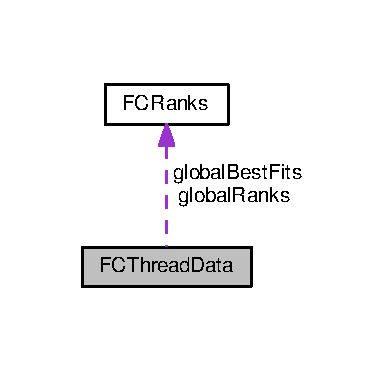
\includegraphics[width=186pt]{structFCThreadData__coll__graph}
\end{center}
\end{figure}
\subsection*{Public Member Functions}
\begin{DoxyCompactItemize}
\item 
\hyperlink{structFCThreadData_a2cf5d9db69def87add57733397912dfa}{F\-C\-Thread\-Data} (boost\-::shared\-\_\-ptr$<$ \hyperlink{classFeldmanCousinsAnalysis}{Feldman\-Cousins\-Analysis} $>$ \hyperlink{structFCThreadData_aab12c7f409e8e59d773d931a4d0b8187}{ana}, \hyperlink{classFCRanks}{F\-C\-Ranks} \&\hyperlink{structFCThreadData_afdceefad89e168d411041e126fa48a0c}{global\-Ranks}, \hyperlink{classFCRanks}{F\-C\-Ranks} \&\hyperlink{structFCThreadData_a8a5d6203aab57c1c05f4d6a2fa549344}{global\-Best\-Fits}, std\-::queue$<$ double $>$ \&\hyperlink{structFCThreadData_a74bbf1a21613e4c77e011a14c1f26c6a}{test\-Hypothesis\-Set}, uint64\-\_\-t \hyperlink{structFCThreadData_a721d95b6dbaeae9dd9a1772794cbc2b2}{n\-Experiments}, uint64\-\_\-t \hyperlink{structFCThreadData_aff011a8ec29fb8962da9474440525374}{thread\-Number}, double \hyperlink{structFCThreadData_a11a41bb60670a5b8a13b3c9dd961d0d0}{cl}, uint64\-\_\-t n\-Hypotheses, uint64\-\_\-t \&\hyperlink{structFCThreadData_ab907b43fdcbc5b14b65cd2ca79306806}{n\-Tested\-Hypotheses})
\end{DoxyCompactItemize}
\subsection*{Public Attributes}
\begin{DoxyCompactItemize}
\item 
boost\-::shared\-\_\-ptr\\*
$<$ \hyperlink{classFeldmanCousinsAnalysis}{Feldman\-Cousins\-Analysis} $>$ \hyperlink{structFCThreadData_aab12c7f409e8e59d773d931a4d0b8187}{ana}
\item 
\hyperlink{classFCRanks}{F\-C\-Ranks} \& \hyperlink{structFCThreadData_afdceefad89e168d411041e126fa48a0c}{global\-Ranks}
\item 
\hyperlink{classFCRanks}{F\-C\-Ranks} \& \hyperlink{structFCThreadData_a8a5d6203aab57c1c05f4d6a2fa549344}{global\-Best\-Fits}
\item 
std\-::queue$<$ double $>$ \& \hyperlink{structFCThreadData_a74bbf1a21613e4c77e011a14c1f26c6a}{test\-Hypothesis\-Set}
\item 
uint64\-\_\-t \hyperlink{structFCThreadData_a721d95b6dbaeae9dd9a1772794cbc2b2}{n\-Experiments}
\item 
uint64\-\_\-t \hyperlink{structFCThreadData_aff011a8ec29fb8962da9474440525374}{thread\-Number}
\item 
double \hyperlink{structFCThreadData_a11a41bb60670a5b8a13b3c9dd961d0d0}{cl}
\item 
uint64\-\_\-t \hyperlink{structFCThreadData_a7243be9f8ba86b1a9f3e6a24b69adfb2}{total\-Hypotheses}
\item 
uint64\-\_\-t \& \hyperlink{structFCThreadData_ab907b43fdcbc5b14b65cd2ca79306806}{n\-Tested\-Hypotheses}
\end{DoxyCompactItemize}


\subsection{Constructor \& Destructor Documentation}
\hypertarget{structFCThreadData_a2cf5d9db69def87add57733397912dfa}{\index{F\-C\-Thread\-Data@{F\-C\-Thread\-Data}!F\-C\-Thread\-Data@{F\-C\-Thread\-Data}}
\index{F\-C\-Thread\-Data@{F\-C\-Thread\-Data}!FCThreadData@{F\-C\-Thread\-Data}}
\subsubsection[{F\-C\-Thread\-Data}]{\setlength{\rightskip}{0pt plus 5cm}F\-C\-Thread\-Data\-::\-F\-C\-Thread\-Data (
\begin{DoxyParamCaption}
\item[{boost\-::shared\-\_\-ptr$<$ {\bf Feldman\-Cousins\-Analysis} $>$}]{ana, }
\item[{{\bf F\-C\-Ranks} \&}]{global\-Ranks, }
\item[{{\bf F\-C\-Ranks} \&}]{global\-Best\-Fits, }
\item[{std\-::queue$<$ double $>$ \&}]{test\-Hypothesis\-Set, }
\item[{uint64\-\_\-t}]{n\-Experiments, }
\item[{uint64\-\_\-t}]{thread\-Number, }
\item[{double}]{cl, }
\item[{uint64\-\_\-t}]{n\-Hypotheses, }
\item[{uint64\-\_\-t \&}]{n\-Tested\-Hypotheses}
\end{DoxyParamCaption}
)\hspace{0.3cm}{\ttfamily [inline]}}}\label{structFCThreadData_a2cf5d9db69def87add57733397912dfa}


\subsection{Member Data Documentation}
\hypertarget{structFCThreadData_aab12c7f409e8e59d773d931a4d0b8187}{\index{F\-C\-Thread\-Data@{F\-C\-Thread\-Data}!ana@{ana}}
\index{ana@{ana}!FCThreadData@{F\-C\-Thread\-Data}}
\subsubsection[{ana}]{\setlength{\rightskip}{0pt plus 5cm}boost\-::shared\-\_\-ptr$<${\bf Feldman\-Cousins\-Analysis}$>$ F\-C\-Thread\-Data\-::ana}}\label{structFCThreadData_aab12c7f409e8e59d773d931a4d0b8187}
\hypertarget{structFCThreadData_a11a41bb60670a5b8a13b3c9dd961d0d0}{\index{F\-C\-Thread\-Data@{F\-C\-Thread\-Data}!cl@{cl}}
\index{cl@{cl}!FCThreadData@{F\-C\-Thread\-Data}}
\subsubsection[{cl}]{\setlength{\rightskip}{0pt plus 5cm}double F\-C\-Thread\-Data\-::cl}}\label{structFCThreadData_a11a41bb60670a5b8a13b3c9dd961d0d0}
\hypertarget{structFCThreadData_a8a5d6203aab57c1c05f4d6a2fa549344}{\index{F\-C\-Thread\-Data@{F\-C\-Thread\-Data}!global\-Best\-Fits@{global\-Best\-Fits}}
\index{global\-Best\-Fits@{global\-Best\-Fits}!FCThreadData@{F\-C\-Thread\-Data}}
\subsubsection[{global\-Best\-Fits}]{\setlength{\rightskip}{0pt plus 5cm}{\bf F\-C\-Ranks}\& F\-C\-Thread\-Data\-::global\-Best\-Fits}}\label{structFCThreadData_a8a5d6203aab57c1c05f4d6a2fa549344}
\hypertarget{structFCThreadData_afdceefad89e168d411041e126fa48a0c}{\index{F\-C\-Thread\-Data@{F\-C\-Thread\-Data}!global\-Ranks@{global\-Ranks}}
\index{global\-Ranks@{global\-Ranks}!FCThreadData@{F\-C\-Thread\-Data}}
\subsubsection[{global\-Ranks}]{\setlength{\rightskip}{0pt plus 5cm}{\bf F\-C\-Ranks}\& F\-C\-Thread\-Data\-::global\-Ranks}}\label{structFCThreadData_afdceefad89e168d411041e126fa48a0c}
\hypertarget{structFCThreadData_a721d95b6dbaeae9dd9a1772794cbc2b2}{\index{F\-C\-Thread\-Data@{F\-C\-Thread\-Data}!n\-Experiments@{n\-Experiments}}
\index{n\-Experiments@{n\-Experiments}!FCThreadData@{F\-C\-Thread\-Data}}
\subsubsection[{n\-Experiments}]{\setlength{\rightskip}{0pt plus 5cm}uint64\-\_\-t F\-C\-Thread\-Data\-::n\-Experiments}}\label{structFCThreadData_a721d95b6dbaeae9dd9a1772794cbc2b2}
\hypertarget{structFCThreadData_ab907b43fdcbc5b14b65cd2ca79306806}{\index{F\-C\-Thread\-Data@{F\-C\-Thread\-Data}!n\-Tested\-Hypotheses@{n\-Tested\-Hypotheses}}
\index{n\-Tested\-Hypotheses@{n\-Tested\-Hypotheses}!FCThreadData@{F\-C\-Thread\-Data}}
\subsubsection[{n\-Tested\-Hypotheses}]{\setlength{\rightskip}{0pt plus 5cm}uint64\-\_\-t\& F\-C\-Thread\-Data\-::n\-Tested\-Hypotheses}}\label{structFCThreadData_ab907b43fdcbc5b14b65cd2ca79306806}
\hypertarget{structFCThreadData_a74bbf1a21613e4c77e011a14c1f26c6a}{\index{F\-C\-Thread\-Data@{F\-C\-Thread\-Data}!test\-Hypothesis\-Set@{test\-Hypothesis\-Set}}
\index{test\-Hypothesis\-Set@{test\-Hypothesis\-Set}!FCThreadData@{F\-C\-Thread\-Data}}
\subsubsection[{test\-Hypothesis\-Set}]{\setlength{\rightskip}{0pt plus 5cm}std\-::queue$<$double$>$\& F\-C\-Thread\-Data\-::test\-Hypothesis\-Set}}\label{structFCThreadData_a74bbf1a21613e4c77e011a14c1f26c6a}
\hypertarget{structFCThreadData_aff011a8ec29fb8962da9474440525374}{\index{F\-C\-Thread\-Data@{F\-C\-Thread\-Data}!thread\-Number@{thread\-Number}}
\index{thread\-Number@{thread\-Number}!FCThreadData@{F\-C\-Thread\-Data}}
\subsubsection[{thread\-Number}]{\setlength{\rightskip}{0pt plus 5cm}uint64\-\_\-t F\-C\-Thread\-Data\-::thread\-Number}}\label{structFCThreadData_aff011a8ec29fb8962da9474440525374}
\hypertarget{structFCThreadData_a7243be9f8ba86b1a9f3e6a24b69adfb2}{\index{F\-C\-Thread\-Data@{F\-C\-Thread\-Data}!total\-Hypotheses@{total\-Hypotheses}}
\index{total\-Hypotheses@{total\-Hypotheses}!FCThreadData@{F\-C\-Thread\-Data}}
\subsubsection[{total\-Hypotheses}]{\setlength{\rightskip}{0pt plus 5cm}uint64\-\_\-t F\-C\-Thread\-Data\-::total\-Hypotheses}}\label{structFCThreadData_a7243be9f8ba86b1a9f3e6a24b69adfb2}


The documentation for this struct was generated from the following file\-:\begin{DoxyCompactItemize}
\item 
/home/travis/build/sflis/\-M\-L\-Sandbox/private/\-M\-L\-Sandbox/\hyperlink{MLSandbox_2FeldmanCousins_8cxx}{Feldman\-Cousins.\-cxx}\end{DoxyCompactItemize}

\hypertarget{classFeldmanCousinsAnalysis}{\section{Feldman\-Cousins\-Analysis Class Reference}
\label{classFeldmanCousinsAnalysis}\index{Feldman\-Cousins\-Analysis@{Feldman\-Cousins\-Analysis}}
}


{\ttfamily \#include $<$Feldman\-Cousins.\-h$>$}



Collaboration diagram for Feldman\-Cousins\-Analysis\-:
\nopagebreak
\begin{figure}[H]
\begin{center}
\leavevmode
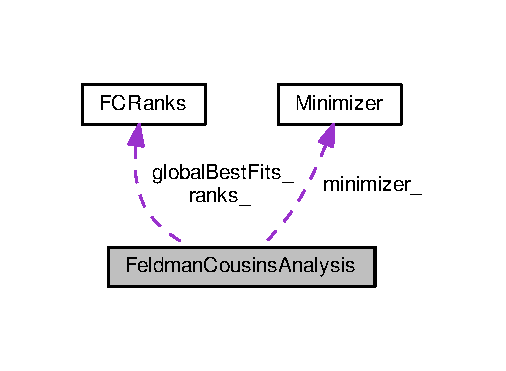
\includegraphics[width=243pt]{classFeldmanCousinsAnalysis__coll__graph}
\end{center}
\end{figure}
\subsection*{Public Member Functions}
\begin{DoxyCompactItemize}
\item 
\hyperlink{classFeldmanCousinsAnalysis_a5b2fbad9a24678ba86f0f5b082a5b726}{Feldman\-Cousins\-Analysis} (boost\-::shared\-\_\-ptr$<$ \hyperlink{classLikelihood}{Likelihood} $>$ llh, double cl)
\item 
double \hyperlink{classFeldmanCousinsAnalysis_a090ca9e45d445fed42345d0a71a589bd}{Evaluate\-Tests\-Statistic} (double xi)
\item 
void \hyperlink{classFeldmanCousinsAnalysis_a5761bf4e0cd5968add070215988517ca}{Set\-F\-C\-Ranks} (\hyperlink{classFCRanks}{F\-C\-Ranks} const \&ranks)
\item 
void \hyperlink{classFeldmanCousinsAnalysis_a0f56a30ad2ec38520aa562fbea7f41cf}{Sample} (double xi)
\item 
void \hyperlink{classFeldmanCousinsAnalysis_a2455d8b563e2f243f02c76d61bf10573}{Generate\-Limits\-Ensemble} (double xi, bn\-::ndarray \&up, bn\-::ndarray \&down, uint64\-\_\-t n\-Experiments, double cl=-\/1)
\item 
void \hyperlink{classFeldmanCousinsAnalysis_ab6d8e4b65fa29c30e248f5e022c28dde}{Compute\-Limits} (double \&upper, double \&lower)
\item 
void \hyperlink{classFeldmanCousinsAnalysis_a0ed46c186508934d827e5fefef53be38}{Compute\-Limits} (double \&upper, double \&lower, bool assume\-Chi2)
\item 
void \hyperlink{classFeldmanCousinsAnalysis_a65c0fb42d70bf0a72b36261cde2ac095}{Compute\-Ranks} (uint64\-\_\-t n\-Experiments, double min\-Xi, double max\-Xi, uint64\-\_\-t n\-Steps, uint64\-\_\-t n\-Threads=1)
\item 
\hyperlink{classFCRanks}{F\-C\-Ranks} \& \hyperlink{classFeldmanCousinsAnalysis_a369111f301236a55ef19aeb7ac0d9562}{Get\-Ranks} ()
\end{DoxyCompactItemize}
\subsection*{Public Attributes}
\begin{DoxyCompactItemize}
\item 
\hyperlink{classFCRanks}{F\-C\-Ranks} \hyperlink{classFeldmanCousinsAnalysis_a2a83aefd21bd62772ba9b8ef2a0afe37}{ranks\-\_\-}
\item 
\hyperlink{classFCRanks}{F\-C\-Ranks} \hyperlink{classFeldmanCousinsAnalysis_a41ab3fd253179cd5fa77b651d4514fdc}{global\-Best\-Fits\-\_\-}
\item 
\hyperlink{classMinimizer}{Minimizer} \hyperlink{classFeldmanCousinsAnalysis_a4a16f04a45c379c10b12f76714116226}{minimizer\-\_\-}
\end{DoxyCompactItemize}


\subsection{Detailed Description}
class\-: \hyperlink{classFeldmanCousinsAnalysis}{Feldman\-Cousins\-Analysis} is a class which encapsulates the F\-C analysis proceedures. 

\subsection{Constructor \& Destructor Documentation}
\hypertarget{classFeldmanCousinsAnalysis_a5b2fbad9a24678ba86f0f5b082a5b726}{\index{Feldman\-Cousins\-Analysis@{Feldman\-Cousins\-Analysis}!Feldman\-Cousins\-Analysis@{Feldman\-Cousins\-Analysis}}
\index{Feldman\-Cousins\-Analysis@{Feldman\-Cousins\-Analysis}!FeldmanCousinsAnalysis@{Feldman\-Cousins\-Analysis}}
\subsubsection[{Feldman\-Cousins\-Analysis}]{\setlength{\rightskip}{0pt plus 5cm}Feldman\-Cousins\-Analysis\-::\-Feldman\-Cousins\-Analysis (
\begin{DoxyParamCaption}
\item[{boost\-::shared\-\_\-ptr$<$ {\bf Likelihood} $>$}]{llh, }
\item[{double}]{cl}
\end{DoxyParamCaption}
)\hspace{0.3cm}{\ttfamily [inline]}}}\label{classFeldmanCousinsAnalysis_a5b2fbad9a24678ba86f0f5b082a5b726}


\subsection{Member Function Documentation}
\hypertarget{classFeldmanCousinsAnalysis_ab6d8e4b65fa29c30e248f5e022c28dde}{\index{Feldman\-Cousins\-Analysis@{Feldman\-Cousins\-Analysis}!Compute\-Limits@{Compute\-Limits}}
\index{Compute\-Limits@{Compute\-Limits}!FeldmanCousinsAnalysis@{Feldman\-Cousins\-Analysis}}
\subsubsection[{Compute\-Limits}]{\setlength{\rightskip}{0pt plus 5cm}void Feldman\-Cousins\-Analysis\-::\-Compute\-Limits (
\begin{DoxyParamCaption}
\item[{double \&}]{upper, }
\item[{double \&}]{lower}
\end{DoxyParamCaption}
)}}\label{classFeldmanCousinsAnalysis_ab6d8e4b65fa29c30e248f5e022c28dde}
\hypertarget{classFeldmanCousinsAnalysis_a0ed46c186508934d827e5fefef53be38}{\index{Feldman\-Cousins\-Analysis@{Feldman\-Cousins\-Analysis}!Compute\-Limits@{Compute\-Limits}}
\index{Compute\-Limits@{Compute\-Limits}!FeldmanCousinsAnalysis@{Feldman\-Cousins\-Analysis}}
\subsubsection[{Compute\-Limits}]{\setlength{\rightskip}{0pt plus 5cm}void Feldman\-Cousins\-Analysis\-::\-Compute\-Limits (
\begin{DoxyParamCaption}
\item[{double \&}]{upper, }
\item[{double \&}]{lower, }
\item[{bool}]{assume\-Chi2}
\end{DoxyParamCaption}
)\hspace{0.3cm}{\ttfamily [inline]}}}\label{classFeldmanCousinsAnalysis_a0ed46c186508934d827e5fefef53be38}
\hypertarget{classFeldmanCousinsAnalysis_a65c0fb42d70bf0a72b36261cde2ac095}{\index{Feldman\-Cousins\-Analysis@{Feldman\-Cousins\-Analysis}!Compute\-Ranks@{Compute\-Ranks}}
\index{Compute\-Ranks@{Compute\-Ranks}!FeldmanCousinsAnalysis@{Feldman\-Cousins\-Analysis}}
\subsubsection[{Compute\-Ranks}]{\setlength{\rightskip}{0pt plus 5cm}void Feldman\-Cousins\-Analysis\-::\-Compute\-Ranks (
\begin{DoxyParamCaption}
\item[{uint64\-\_\-t}]{n\-Experiments, }
\item[{double}]{min\-Xi, }
\item[{double}]{max\-Xi, }
\item[{uint64\-\_\-t}]{n\-Steps, }
\item[{uint64\-\_\-t}]{n\-Threads = {\ttfamily 1}}
\end{DoxyParamCaption}
)}}\label{classFeldmanCousinsAnalysis_a65c0fb42d70bf0a72b36261cde2ac095}
\hypertarget{classFeldmanCousinsAnalysis_a090ca9e45d445fed42345d0a71a589bd}{\index{Feldman\-Cousins\-Analysis@{Feldman\-Cousins\-Analysis}!Evaluate\-Tests\-Statistic@{Evaluate\-Tests\-Statistic}}
\index{Evaluate\-Tests\-Statistic@{Evaluate\-Tests\-Statistic}!FeldmanCousinsAnalysis@{Feldman\-Cousins\-Analysis}}
\subsubsection[{Evaluate\-Tests\-Statistic}]{\setlength{\rightskip}{0pt plus 5cm}double Feldman\-Cousins\-Analysis\-::\-Evaluate\-Tests\-Statistic (
\begin{DoxyParamCaption}
\item[{double}]{xi}
\end{DoxyParamCaption}
)\hspace{0.3cm}{\ttfamily [inline]}}}\label{classFeldmanCousinsAnalysis_a090ca9e45d445fed42345d0a71a589bd}
Returns the log value of the F\-C test-\/statistic for a given likelihood parameter 
\begin{DoxyParams}{Parameters}
{\em xi} & likelihood parameter for which the test statistic should be calculated \\
\hline
\end{DoxyParams}
\begin{DoxyReturn}{Returns}
the log of the F\-C test-\/statistic = log(L(xi)/\-L(xi\-\_\-best)) 
\end{DoxyReturn}
\hypertarget{classFeldmanCousinsAnalysis_a2455d8b563e2f243f02c76d61bf10573}{\index{Feldman\-Cousins\-Analysis@{Feldman\-Cousins\-Analysis}!Generate\-Limits\-Ensemble@{Generate\-Limits\-Ensemble}}
\index{Generate\-Limits\-Ensemble@{Generate\-Limits\-Ensemble}!FeldmanCousinsAnalysis@{Feldman\-Cousins\-Analysis}}
\subsubsection[{Generate\-Limits\-Ensemble}]{\setlength{\rightskip}{0pt plus 5cm}void Feldman\-Cousins\-Analysis\-::\-Generate\-Limits\-Ensemble (
\begin{DoxyParamCaption}
\item[{double}]{xi, }
\item[{bn\-::ndarray \&}]{up, }
\item[{bn\-::ndarray \&}]{down, }
\item[{uint64\-\_\-t}]{n\-Experiments, }
\item[{double}]{cl = {\ttfamily -\/1}}
\end{DoxyParamCaption}
)}}\label{classFeldmanCousinsAnalysis_a2455d8b563e2f243f02c76d61bf10573}
Generates an ensemble of pseudo experiments to construct upper and lower limits distributions at a given likelihood parameter value xi 
\begin{DoxyParams}{Parameters}
{\em xi} & \\
\hline
{\em up} & \\
\hline
{\em down} & \\
\hline
{\em cl} & \\
\hline
{\em n\-Experiments} & \\
\hline
\end{DoxyParams}
\hypertarget{classFeldmanCousinsAnalysis_a369111f301236a55ef19aeb7ac0d9562}{\index{Feldman\-Cousins\-Analysis@{Feldman\-Cousins\-Analysis}!Get\-Ranks@{Get\-Ranks}}
\index{Get\-Ranks@{Get\-Ranks}!FeldmanCousinsAnalysis@{Feldman\-Cousins\-Analysis}}
\subsubsection[{Get\-Ranks}]{\setlength{\rightskip}{0pt plus 5cm}{\bf F\-C\-Ranks}\& Feldman\-Cousins\-Analysis\-::\-Get\-Ranks (
\begin{DoxyParamCaption}
{}
\end{DoxyParamCaption}
)\hspace{0.3cm}{\ttfamily [inline]}}}\label{classFeldmanCousinsAnalysis_a369111f301236a55ef19aeb7ac0d9562}
\hypertarget{classFeldmanCousinsAnalysis_a0f56a30ad2ec38520aa562fbea7f41cf}{\index{Feldman\-Cousins\-Analysis@{Feldman\-Cousins\-Analysis}!Sample@{Sample}}
\index{Sample@{Sample}!FeldmanCousinsAnalysis@{Feldman\-Cousins\-Analysis}}
\subsubsection[{Sample}]{\setlength{\rightskip}{0pt plus 5cm}void Feldman\-Cousins\-Analysis\-::\-Sample (
\begin{DoxyParamCaption}
\item[{double}]{xi}
\end{DoxyParamCaption}
)\hspace{0.3cm}{\ttfamily [inline]}}}\label{classFeldmanCousinsAnalysis_a0f56a30ad2ec38520aa562fbea7f41cf}
\hypertarget{classFeldmanCousinsAnalysis_a5761bf4e0cd5968add070215988517ca}{\index{Feldman\-Cousins\-Analysis@{Feldman\-Cousins\-Analysis}!Set\-F\-C\-Ranks@{Set\-F\-C\-Ranks}}
\index{Set\-F\-C\-Ranks@{Set\-F\-C\-Ranks}!FeldmanCousinsAnalysis@{Feldman\-Cousins\-Analysis}}
\subsubsection[{Set\-F\-C\-Ranks}]{\setlength{\rightskip}{0pt plus 5cm}void Feldman\-Cousins\-Analysis\-::\-Set\-F\-C\-Ranks (
\begin{DoxyParamCaption}
\item[{{\bf F\-C\-Ranks} const \&}]{ranks}
\end{DoxyParamCaption}
)\hspace{0.3cm}{\ttfamily [inline]}}}\label{classFeldmanCousinsAnalysis_a5761bf4e0cd5968add070215988517ca}


\subsection{Member Data Documentation}
\hypertarget{classFeldmanCousinsAnalysis_a41ab3fd253179cd5fa77b651d4514fdc}{\index{Feldman\-Cousins\-Analysis@{Feldman\-Cousins\-Analysis}!global\-Best\-Fits\-\_\-@{global\-Best\-Fits\-\_\-}}
\index{global\-Best\-Fits\-\_\-@{global\-Best\-Fits\-\_\-}!FeldmanCousinsAnalysis@{Feldman\-Cousins\-Analysis}}
\subsubsection[{global\-Best\-Fits\-\_\-}]{\setlength{\rightskip}{0pt plus 5cm}{\bf F\-C\-Ranks} Feldman\-Cousins\-Analysis\-::global\-Best\-Fits\-\_\-}}\label{classFeldmanCousinsAnalysis_a41ab3fd253179cd5fa77b651d4514fdc}
\hypertarget{classFeldmanCousinsAnalysis_a4a16f04a45c379c10b12f76714116226}{\index{Feldman\-Cousins\-Analysis@{Feldman\-Cousins\-Analysis}!minimizer\-\_\-@{minimizer\-\_\-}}
\index{minimizer\-\_\-@{minimizer\-\_\-}!FeldmanCousinsAnalysis@{Feldman\-Cousins\-Analysis}}
\subsubsection[{minimizer\-\_\-}]{\setlength{\rightskip}{0pt plus 5cm}{\bf Minimizer} Feldman\-Cousins\-Analysis\-::minimizer\-\_\-}}\label{classFeldmanCousinsAnalysis_a4a16f04a45c379c10b12f76714116226}
\hypertarget{classFeldmanCousinsAnalysis_a2a83aefd21bd62772ba9b8ef2a0afe37}{\index{Feldman\-Cousins\-Analysis@{Feldman\-Cousins\-Analysis}!ranks\-\_\-@{ranks\-\_\-}}
\index{ranks\-\_\-@{ranks\-\_\-}!FeldmanCousinsAnalysis@{Feldman\-Cousins\-Analysis}}
\subsubsection[{ranks\-\_\-}]{\setlength{\rightskip}{0pt plus 5cm}{\bf F\-C\-Ranks} Feldman\-Cousins\-Analysis\-::ranks\-\_\-}}\label{classFeldmanCousinsAnalysis_a2a83aefd21bd62772ba9b8ef2a0afe37}


The documentation for this class was generated from the following files\-:\begin{DoxyCompactItemize}
\item 
/home/travis/build/sflis/\-M\-L\-Sandbox/public/\-M\-L\-Sandbox/\hyperlink{FeldmanCousins_8h}{Feldman\-Cousins.\-h}\item 
/home/travis/build/sflis/\-M\-L\-Sandbox/private/\-M\-L\-Sandbox/\hyperlink{MLSandbox_2FeldmanCousins_8cxx}{Feldman\-Cousins.\-cxx}\end{DoxyCompactItemize}

\hypertarget{structjob}{\section{job Struct Reference}
\label{structjob}\index{job@{job}}
}
\subsection*{Public Member Functions}
\begin{DoxyCompactItemize}
\item 
\hyperlink{structjob_a3720c8881d35e41c2d2a22f1f1bcd02f}{job} (double \hyperlink{structjob_a97b527f70afea9c220bf6af904e5ca06}{hypo}=0, uint64\-\_\-t \hyperlink{structjob_a3145a4e74a386b4a1922794dc2739410}{n\-Experiments}=0, bool \hyperlink{structjob_a4ab7aa6c5bd6a19b3da8e4387353ea96}{last}=false)
\end{DoxyCompactItemize}
\subsection*{Public Attributes}
\begin{DoxyCompactItemize}
\item 
double \hyperlink{structjob_a97b527f70afea9c220bf6af904e5ca06}{hypo}
\item 
uint64\-\_\-t \hyperlink{structjob_a3145a4e74a386b4a1922794dc2739410}{n\-Experiments}
\item 
bool \hyperlink{structjob_a4ab7aa6c5bd6a19b3da8e4387353ea96}{last}
\end{DoxyCompactItemize}


\subsection{Constructor \& Destructor Documentation}
\hypertarget{structjob_a3720c8881d35e41c2d2a22f1f1bcd02f}{\index{job@{job}!job@{job}}
\index{job@{job}!job@{job}}
\subsubsection[{job}]{\setlength{\rightskip}{0pt plus 5cm}job\-::job (
\begin{DoxyParamCaption}
\item[{double}]{hypo = {\ttfamily 0}, }
\item[{uint64\-\_\-t}]{n\-Experiments = {\ttfamily 0}, }
\item[{bool}]{last = {\ttfamily false}}
\end{DoxyParamCaption}
)\hspace{0.3cm}{\ttfamily [inline]}}}\label{structjob_a3720c8881d35e41c2d2a22f1f1bcd02f}


\subsection{Member Data Documentation}
\hypertarget{structjob_a97b527f70afea9c220bf6af904e5ca06}{\index{job@{job}!hypo@{hypo}}
\index{hypo@{hypo}!job@{job}}
\subsubsection[{hypo}]{\setlength{\rightskip}{0pt plus 5cm}double job\-::hypo}}\label{structjob_a97b527f70afea9c220bf6af904e5ca06}
\hypertarget{structjob_a4ab7aa6c5bd6a19b3da8e4387353ea96}{\index{job@{job}!last@{last}}
\index{last@{last}!job@{job}}
\subsubsection[{last}]{\setlength{\rightskip}{0pt plus 5cm}bool job\-::last}}\label{structjob_a4ab7aa6c5bd6a19b3da8e4387353ea96}
\hypertarget{structjob_a3145a4e74a386b4a1922794dc2739410}{\index{job@{job}!n\-Experiments@{n\-Experiments}}
\index{n\-Experiments@{n\-Experiments}!job@{job}}
\subsubsection[{n\-Experiments}]{\setlength{\rightskip}{0pt plus 5cm}uint64\-\_\-t job\-::n\-Experiments}}\label{structjob_a3145a4e74a386b4a1922794dc2739410}


The documentation for this struct was generated from the following file\-:\begin{DoxyCompactItemize}
\item 
/home/travis/build/sflis/\-M\-L\-Sandbox/private/\-M\-L\-Sandbox/\hyperlink{MLSandbox_2NeymanAnalysis_8cxx}{Neyman\-Analysis.\-cxx}\end{DoxyCompactItemize}

\hypertarget{classLikelihood}{\section{Likelihood Class Reference}
\label{classLikelihood}\index{Likelihood@{Likelihood}}
}


A base class (wrapper class) for likelihoods which defines a general interface needed analysis classes.  




{\ttfamily \#include $<$Likelihood.\-h$>$}



Inheritance diagram for Likelihood\-:
\nopagebreak
\begin{figure}[H]
\begin{center}
\leavevmode
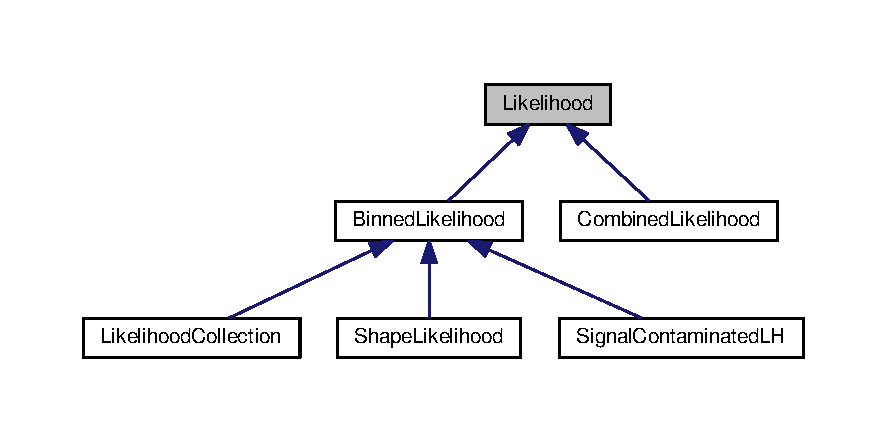
\includegraphics[width=350pt]{classLikelihood__inherit__graph}
\end{center}
\end{figure}
\subsection*{Public Member Functions}
\begin{DoxyCompactItemize}
\item 
virtual double \hyperlink{classLikelihood_ab8dd44247a393aa203ff3513b2ba1587}{Evaluate\-L\-L\-H} (double xi) const =0
\item 
virtual void \hyperlink{classLikelihood_a11245b8594fa8658698798d92a56e4d8}{Sample\-Events} (double xi)=0
\item 
virtual \hyperlink{Likelihood_8h_a97d92c5c141f28319e7e8198defc9084}{likelihood\-Callback} \hyperlink{classLikelihood_a423872ac038f3fc30d0080f199dc1feb}{Call\-Back\-Fcn} ()=0
\item 
virtual \hyperlink{classLikelihood}{Likelihood} $\ast$ \hyperlink{classLikelihood_a938b362a171c46f447cb364effc83bcf}{Clone} (int seed) const =0
\item 
virtual void \hyperlink{classLikelihood_ae43d17adaa0b34b9da4948e262b8d898}{Minimizer\-Conditions} (\hyperlink{classMinimizer}{Minimizer} \&min)
\item 
virtual bool \hyperlink{classLikelihood_a48cfa022b87027e4793dac6fa0dd1b24}{Changed} ()
\item 
virtual double \hyperlink{classLikelihood_a5af640d09a81f553b8331d2557b01aa6}{Min\-Xi\-Bound} ()
\item 
virtual double \hyperlink{classLikelihood_a948c31dcc4fe8efc7c39db49ad56c745}{Max\-Xi\-Bound} ()
\item 
virtual uint32\-\_\-t \hyperlink{classLikelihood_a5e38ffabbfeba8196b71073effc497c9}{State\-Hash} ()=0
\begin{DoxyCompactList}\small\item\em Returns a hash number of the observation. \end{DoxyCompactList}\end{DoxyCompactItemize}
\subsection*{Public Attributes}
\begin{DoxyCompactItemize}
\item 
uint64\-\_\-t \hyperlink{classLikelihood_afc00e95dfa5a5c71d413830f50958d80}{tot\-Events\-\_\-}
\begin{DoxyCompactList}\small\item\em Number of events in the current sample. \end{DoxyCompactList}\item 
double \hyperlink{classLikelihood_afa1482c93235340101bb2d6ad9398f60}{N\-\_\-}
\begin{DoxyCompactList}\small\item\em Expected number of events in the sample. \end{DoxyCompactList}\end{DoxyCompactItemize}
\subsection*{Protected Attributes}
\begin{DoxyCompactItemize}
\item 
bool \hyperlink{classLikelihood_afb7ebdce4ecd44b62bf5573ac3a96562}{changed\-\_\-}
\item 
uint32\-\_\-t \hyperlink{classLikelihood_a9a9940bdd1aa6ee5efd8da4a883c3d79}{state\-Hash\-\_\-}
\end{DoxyCompactItemize}


\subsection{Detailed Description}
A base class (wrapper class) for likelihoods which defines a general interface needed analysis classes. 

class\-: \hyperlink{classLikelihood}{Likelihood} 

\subsection{Member Function Documentation}
\hypertarget{classLikelihood_a423872ac038f3fc30d0080f199dc1feb}{\index{Likelihood@{Likelihood}!Call\-Back\-Fcn@{Call\-Back\-Fcn}}
\index{Call\-Back\-Fcn@{Call\-Back\-Fcn}!Likelihood@{Likelihood}}
\subsubsection[{Call\-Back\-Fcn}]{\setlength{\rightskip}{0pt plus 5cm}virtual {\bf likelihood\-Callback} Likelihood\-::\-Call\-Back\-Fcn (
\begin{DoxyParamCaption}
{}
\end{DoxyParamCaption}
)\hspace{0.3cm}{\ttfamily [pure virtual]}}}\label{classLikelihood_a423872ac038f3fc30d0080f199dc1feb}
Return the callback function of the likelihood for the minimizer \begin{DoxyReturn}{Returns}
A function pointer function of the type double(double,void$\ast$) 
\end{DoxyReturn}


Implemented in \hyperlink{classShapeLikelihood_acf56e312fd4f0881aa09215d73b93412}{Shape\-Likelihood}, \hyperlink{classBinnedLikelihood_aed7e05d58a36f515afc8e34fe8550b31}{Binned\-Likelihood}, \hyperlink{classLikelihoodCollection_af4c889ced5fc4de6be4ffac2898250b5}{Likelihood\-Collection}, \hyperlink{classSignalContaminatedLH_a9c67422f6e79df2352bd158be9949feb}{Signal\-Contaminated\-L\-H}, and \hyperlink{classCombinedLikelihood_a4d70d16e3f63005427dc9261addd0bfb}{Combined\-Likelihood}.

\hypertarget{classLikelihood_a48cfa022b87027e4793dac6fa0dd1b24}{\index{Likelihood@{Likelihood}!Changed@{Changed}}
\index{Changed@{Changed}!Likelihood@{Likelihood}}
\subsubsection[{Changed}]{\setlength{\rightskip}{0pt plus 5cm}virtual bool Likelihood\-::\-Changed (
\begin{DoxyParamCaption}
{}
\end{DoxyParamCaption}
)\hspace{0.3cm}{\ttfamily [inline]}, {\ttfamily [virtual]}}}\label{classLikelihood_a48cfa022b87027e4793dac6fa0dd1b24}
Returns true if the state of the likelihood has changed since the last call to Change indicating that the event sample of the likelihood might have changed thus a recalculation of the best fit is needed. \hypertarget{classLikelihood_a938b362a171c46f447cb364effc83bcf}{\index{Likelihood@{Likelihood}!Clone@{Clone}}
\index{Clone@{Clone}!Likelihood@{Likelihood}}
\subsubsection[{Clone}]{\setlength{\rightskip}{0pt plus 5cm}virtual {\bf Likelihood}$\ast$ Likelihood\-::\-Clone (
\begin{DoxyParamCaption}
\item[{int}]{seed}
\end{DoxyParamCaption}
) const\hspace{0.3cm}{\ttfamily [pure virtual]}}}\label{classLikelihood_a938b362a171c46f447cb364effc83bcf}
Should create a copy of the original \hyperlink{classLikelihood}{Likelihood} which is thread safe. 

Implemented in \hyperlink{classShapeLikelihood_a67630eb790d07ef1d0d2e33711495cbe}{Shape\-Likelihood}, \hyperlink{classLikelihoodCollection_ae3d80984323771199c511db7016608cf}{Likelihood\-Collection}, \hyperlink{classSignalContaminatedLH_ae7c8264a79340a12dd4a83d83f0b9d2f}{Signal\-Contaminated\-L\-H}, and \hyperlink{classCombinedLikelihood_afb2505b9b126ddfcc859b150e8345aed}{Combined\-Likelihood}.

\hypertarget{classLikelihood_ab8dd44247a393aa203ff3513b2ba1587}{\index{Likelihood@{Likelihood}!Evaluate\-L\-L\-H@{Evaluate\-L\-L\-H}}
\index{Evaluate\-L\-L\-H@{Evaluate\-L\-L\-H}!Likelihood@{Likelihood}}
\subsubsection[{Evaluate\-L\-L\-H}]{\setlength{\rightskip}{0pt plus 5cm}virtual double Likelihood\-::\-Evaluate\-L\-L\-H (
\begin{DoxyParamCaption}
\item[{double}]{xi}
\end{DoxyParamCaption}
) const\hspace{0.3cm}{\ttfamily [pure virtual]}}}\label{classLikelihood_ab8dd44247a393aa203ff3513b2ba1587}
Evaluates the log likelihood sum 
\begin{DoxyParams}{Parameters}
{\em xi} & the signal fraction for which the likelihood should be evaulated. \\
\hline
\end{DoxyParams}


Implemented in \hyperlink{classShapeLikelihood_afe024bedaab4633ded018d23d17c37f8}{Shape\-Likelihood}, \hyperlink{classBinnedLikelihood_a2084a64cd8b5d6bf8055538a0f633785}{Binned\-Likelihood}, \hyperlink{classLikelihoodCollection_a942b79738d2be74a358e138ff5284f53}{Likelihood\-Collection}, \hyperlink{classSignalContaminatedLH_a30c729fa905cc0d812827f23c71b55cc}{Signal\-Contaminated\-L\-H}, and \hyperlink{classCombinedLikelihood_a5d41f29fd87fcab976a06e0af12e6767}{Combined\-Likelihood}.

\hypertarget{classLikelihood_a948c31dcc4fe8efc7c39db49ad56c745}{\index{Likelihood@{Likelihood}!Max\-Xi\-Bound@{Max\-Xi\-Bound}}
\index{Max\-Xi\-Bound@{Max\-Xi\-Bound}!Likelihood@{Likelihood}}
\subsubsection[{Max\-Xi\-Bound}]{\setlength{\rightskip}{0pt plus 5cm}virtual double Likelihood\-::\-Max\-Xi\-Bound (
\begin{DoxyParamCaption}
{}
\end{DoxyParamCaption}
)\hspace{0.3cm}{\ttfamily [inline]}, {\ttfamily [virtual]}}}\label{classLikelihood_a948c31dcc4fe8efc7c39db49ad56c745}


Reimplemented in \hyperlink{classBinnedLikelihood_ab6144b4d092744dc9d5ee58a491bf77d}{Binned\-Likelihood}, \hyperlink{classLikelihoodCollection_adc81d79fce77d226853f4cfcb33fb7a3}{Likelihood\-Collection}, \hyperlink{classSignalContaminatedLH_a579d86a266c6ecb44cff26e47d141a9e}{Signal\-Contaminated\-L\-H}, and \hyperlink{classCombinedLikelihood_a2cf396d545d7873be85a9bbcb72f4b53}{Combined\-Likelihood}.

\hypertarget{classLikelihood_ae43d17adaa0b34b9da4948e262b8d898}{\index{Likelihood@{Likelihood}!Minimizer\-Conditions@{Minimizer\-Conditions}}
\index{Minimizer\-Conditions@{Minimizer\-Conditions}!Likelihood@{Likelihood}}
\subsubsection[{Minimizer\-Conditions}]{\setlength{\rightskip}{0pt plus 5cm}virtual void Likelihood\-::\-Minimizer\-Conditions (
\begin{DoxyParamCaption}
\item[{{\bf Minimizer} \&}]{min}
\end{DoxyParamCaption}
)\hspace{0.3cm}{\ttfamily [inline]}, {\ttfamily [virtual]}}}\label{classLikelihood_ae43d17adaa0b34b9da4948e262b8d898}


Reimplemented in \hyperlink{classLikelihoodCollection_ae1d445fbfc327da63d469d67891dc7e3}{Likelihood\-Collection}, and \hyperlink{classSignalContaminatedLH_ad991e7649ed72c411830cb0c7788dff4}{Signal\-Contaminated\-L\-H}.

\hypertarget{classLikelihood_a5af640d09a81f553b8331d2557b01aa6}{\index{Likelihood@{Likelihood}!Min\-Xi\-Bound@{Min\-Xi\-Bound}}
\index{Min\-Xi\-Bound@{Min\-Xi\-Bound}!Likelihood@{Likelihood}}
\subsubsection[{Min\-Xi\-Bound}]{\setlength{\rightskip}{0pt plus 5cm}virtual double Likelihood\-::\-Min\-Xi\-Bound (
\begin{DoxyParamCaption}
{}
\end{DoxyParamCaption}
)\hspace{0.3cm}{\ttfamily [inline]}, {\ttfamily [virtual]}}}\label{classLikelihood_a5af640d09a81f553b8331d2557b01aa6}


Reimplemented in \hyperlink{classBinnedLikelihood_a16f5c7acb008393fcdb12df2524d7033}{Binned\-Likelihood}.

\hypertarget{classLikelihood_a11245b8594fa8658698798d92a56e4d8}{\index{Likelihood@{Likelihood}!Sample\-Events@{Sample\-Events}}
\index{Sample\-Events@{Sample\-Events}!Likelihood@{Likelihood}}
\subsubsection[{Sample\-Events}]{\setlength{\rightskip}{0pt plus 5cm}virtual void Likelihood\-::\-Sample\-Events (
\begin{DoxyParamCaption}
\item[{double}]{xi}
\end{DoxyParamCaption}
)\hspace{0.3cm}{\ttfamily [pure virtual]}}}\label{classLikelihood_a11245b8594fa8658698798d92a56e4d8}
Creates internally a new sample with the specified parameter likelihood parameter 
\begin{DoxyParams}{Parameters}
{\em xi} & value of the likelihood parameter \\
\hline
\end{DoxyParams}


Implemented in \hyperlink{classShapeLikelihood_aa303861500c399cb680d89b15d08b806}{Shape\-Likelihood}, \hyperlink{classBinnedLikelihood_a0793b8109912c6e509470a14a58d2a2a}{Binned\-Likelihood}, \hyperlink{classLikelihoodCollection_a38af4d60e248c8d32d0b05ce623c031b}{Likelihood\-Collection}, \hyperlink{classSignalContaminatedLH_a04fcf69547f8b0c5bc3ee2cb89671c06}{Signal\-Contaminated\-L\-H}, and \hyperlink{classCombinedLikelihood_a2e3dc150595fdab805b77fc8f2557fa0}{Combined\-Likelihood}.

\hypertarget{classLikelihood_a5e38ffabbfeba8196b71073effc497c9}{\index{Likelihood@{Likelihood}!State\-Hash@{State\-Hash}}
\index{State\-Hash@{State\-Hash}!Likelihood@{Likelihood}}
\subsubsection[{State\-Hash}]{\setlength{\rightskip}{0pt plus 5cm}virtual uint32\-\_\-t Likelihood\-::\-State\-Hash (
\begin{DoxyParamCaption}
{}
\end{DoxyParamCaption}
)\hspace{0.3cm}{\ttfamily [pure virtual]}}}\label{classLikelihood_a5e38ffabbfeba8196b71073effc497c9}


Returns a hash number of the observation. 



Implemented in \hyperlink{classBinnedLikelihood_a8b6371a5da5acc90bc1d601422bb9764}{Binned\-Likelihood}, and \hyperlink{classCombinedLikelihood_a7980d2517a55eea72e7e272917b1948d}{Combined\-Likelihood}.



\subsection{Member Data Documentation}
\hypertarget{classLikelihood_afb7ebdce4ecd44b62bf5573ac3a96562}{\index{Likelihood@{Likelihood}!changed\-\_\-@{changed\-\_\-}}
\index{changed\-\_\-@{changed\-\_\-}!Likelihood@{Likelihood}}
\subsubsection[{changed\-\_\-}]{\setlength{\rightskip}{0pt plus 5cm}bool Likelihood\-::changed\-\_\-\hspace{0.3cm}{\ttfamily [protected]}}}\label{classLikelihood_afb7ebdce4ecd44b62bf5573ac3a96562}
\hypertarget{classLikelihood_afa1482c93235340101bb2d6ad9398f60}{\index{Likelihood@{Likelihood}!N\-\_\-@{N\-\_\-}}
\index{N\-\_\-@{N\-\_\-}!Likelihood@{Likelihood}}
\subsubsection[{N\-\_\-}]{\setlength{\rightskip}{0pt plus 5cm}double Likelihood\-::\-N\-\_\-}}\label{classLikelihood_afa1482c93235340101bb2d6ad9398f60}


Expected number of events in the sample. 

\hypertarget{classLikelihood_a9a9940bdd1aa6ee5efd8da4a883c3d79}{\index{Likelihood@{Likelihood}!state\-Hash\-\_\-@{state\-Hash\-\_\-}}
\index{state\-Hash\-\_\-@{state\-Hash\-\_\-}!Likelihood@{Likelihood}}
\subsubsection[{state\-Hash\-\_\-}]{\setlength{\rightskip}{0pt plus 5cm}uint32\-\_\-t Likelihood\-::state\-Hash\-\_\-\hspace{0.3cm}{\ttfamily [protected]}}}\label{classLikelihood_a9a9940bdd1aa6ee5efd8da4a883c3d79}
\hypertarget{classLikelihood_afc00e95dfa5a5c71d413830f50958d80}{\index{Likelihood@{Likelihood}!tot\-Events\-\_\-@{tot\-Events\-\_\-}}
\index{tot\-Events\-\_\-@{tot\-Events\-\_\-}!Likelihood@{Likelihood}}
\subsubsection[{tot\-Events\-\_\-}]{\setlength{\rightskip}{0pt plus 5cm}uint64\-\_\-t Likelihood\-::tot\-Events\-\_\-}}\label{classLikelihood_afc00e95dfa5a5c71d413830f50958d80}


Number of events in the current sample. 



The documentation for this class was generated from the following file\-:\begin{DoxyCompactItemize}
\item 
/home/travis/build/sflis/\-M\-L\-Sandbox/public/\-M\-L\-Sandbox/\hyperlink{Likelihood_8h}{Likelihood.\-h}\end{DoxyCompactItemize}

\hypertarget{classLikelihoodCollection}{\section{Likelihood\-Collection Class Reference}
\label{classLikelihoodCollection}\index{Likelihood\-Collection@{Likelihood\-Collection}}
}


{\ttfamily \#include $<$Likelihood\-Collection.\-h$>$}



Inheritance diagram for Likelihood\-Collection\-:
\nopagebreak
\begin{figure}[H]
\begin{center}
\leavevmode
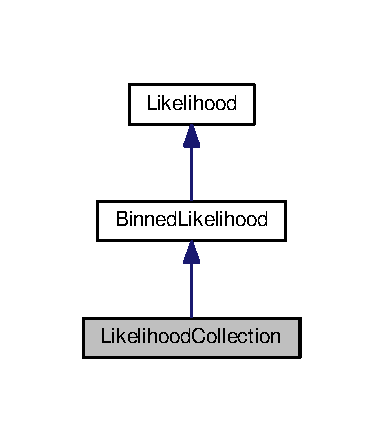
\includegraphics[width=184pt]{classLikelihoodCollection__inherit__graph}
\end{center}
\end{figure}


Collaboration diagram for Likelihood\-Collection\-:
\nopagebreak
\begin{figure}[H]
\begin{center}
\leavevmode
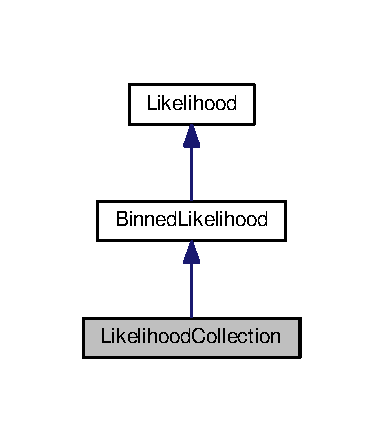
\includegraphics[width=184pt]{classLikelihoodCollection__coll__graph}
\end{center}
\end{figure}
\subsection*{Public Types}
\begin{DoxyCompactItemize}
\item 
enum \hyperlink{classLikelihoodCollection_a3d71df2ed0bdff414ae5fedb30f7cc76}{Model} \{ \hyperlink{classLikelihoodCollection_a3d71df2ed0bdff414ae5fedb30f7cc76a1f3fa362dbbf13c3fa8c732c6125b040}{None}, 
\hyperlink{classLikelihoodCollection_a3d71df2ed0bdff414ae5fedb30f7cc76afdc2c0395310f3e3a033a8b4239c5927}{Poisson}, 
\hyperlink{classLikelihoodCollection_a3d71df2ed0bdff414ae5fedb30f7cc76aea62206336d47863916f4eaa6dc99662}{Binomial}
 \}
\end{DoxyCompactItemize}
\subsection*{Public Member Functions}
\begin{DoxyCompactItemize}
\item 
\hyperlink{classLikelihoodCollection_acde8a81497f959a7b6af883490da0bd7}{Likelihood\-Collection} (const \hyperlink{classDistribution}{Distribution} \&signal, const \hyperlink{classDistribution}{Distribution} \&background, const \hyperlink{classDistribution}{Distribution} \&signal\-Scrambled, const \hyperlink{classDistribution}{Distribution} \&signal\-Sample, const \hyperlink{classDistribution}{Distribution} \&background\-Sample, const \hyperlink{classDistribution}{Distribution} \&signal\-Scrambled\-Sample, double N, double sig\-\_\-prob=1.\-0, double bg\-\_\-prob=1.\-0, \hyperlink{classLikelihoodCollection_a3d71df2ed0bdff414ae5fedb30f7cc76}{Likelihood\-Collection\-::\-Model} model=\hyperlink{classLikelihoodCollection_a3d71df2ed0bdff414ae5fedb30f7cc76a1f3fa362dbbf13c3fa8c732c6125b040}{Likelihood\-Collection\-::\-None}, double sig\-\_\-sample\-\_\-prob=1.\-0, double bg\-\_\-sample\-\_\-prob=1.\-0, int seed=1)
\item 
double \hyperlink{classLikelihoodCollection_a942b79738d2be74a358e138ff5284f53}{Evaluate\-L\-L\-H} (double xi) const 
\item 
double \hyperlink{classLikelihoodCollection_a72f0fc31317f33ad79cba87753ce736e}{No\-Sig\-Sub\-Corr} (double xi) const 
\item 
double \hyperlink{classLikelihoodCollection_a18f2600065b936215bea7c4eb223b548}{Standard\-Sig\-Sub} (double xi) const 
\item 
\hyperlink{classLikelihoodCollection_a3d71df2ed0bdff414ae5fedb30f7cc76}{Model} \hyperlink{classLikelihoodCollection_ad59da7f036985775d8c81caeaa8e461b}{Get\-Model} ()
\item 
const \hyperlink{classDistribution}{Distribution} \& \hyperlink{classLikelihoodCollection_acd787cbdd7ca9dbdc09bb2ec1972e29d}{Get\-Signal\-P\-D\-F} () const 
\item 
const \hyperlink{classDistribution}{Distribution} \& \hyperlink{classLikelihoodCollection_a1421a10716bb315e62c14ae325ed8311}{Get\-Bg\-P\-D\-F} () const 
\item 
void \hyperlink{classLikelihoodCollection_a38af4d60e248c8d32d0b05ce623c031b}{Sample\-Events} (double xi)
\begin{DoxyCompactList}\small\item\em Creates internally a new sample with the specified parameter. \end{DoxyCompactList}\item 
uint64\-\_\-t \hyperlink{classLikelihoodCollection_ad6a6c6a4549d33052f1a0256c1bee059}{Get\-N\-Events} ()
\item 
double \hyperlink{classLikelihoodCollection_a794f0baef8300c86905d22e92f9a157e}{Xi2\-W} (double xi) const 
\item 
double \hyperlink{classLikelihoodCollection_a9a1ca7a817d25f9e01d65c4015111ebe}{W2\-Xi} (double w) const 
\item 
double \hyperlink{classLikelihoodCollection_a72719241eded381680815ebdda1e6502}{W2\-Mu} (double w) const 
\item 
double \hyperlink{classLikelihoodCollection_ac7dcd857dcbbe516e9b83a1405422cfb}{Xi2\-Mu} (double xi) const 
\item 
double \hyperlink{classLikelihoodCollection_ad4009a5ffe924948b39d760c9f31f5c3}{Mu2\-Xi} (double mu) const 
\item 
void \hyperlink{classLikelihoodCollection_ae1d445fbfc327da63d469d67891dc7e3}{Minimizer\-Conditions} (\hyperlink{classMinimizer}{Minimizer} \&min)
\item 
\hyperlink{Likelihood_8h_a97d92c5c141f28319e7e8198defc9084}{likelihood\-Callback} \hyperlink{classLikelihoodCollection_af4c889ced5fc4de6be4ffac2898250b5}{Call\-Back\-Fcn} ()
\begin{DoxyCompactList}\small\item\em Return the callback function of the likelihood for the minimizer. \end{DoxyCompactList}\item 
\hyperlink{classLikelihoodCollection}{Likelihood\-Collection} $\ast$ \hyperlink{classLikelihoodCollection_ae3d80984323771199c511db7016608cf}{Clone} (int seed) const 
\item 
double \hyperlink{classLikelihoodCollection_adc81d79fce77d226853f4cfcb33fb7a3}{Max\-Xi\-Bound} ()
\item 
void \hyperlink{classLikelihoodCollection_ade325e0d8eb68213933bf19ea83f8276}{Set\-L\-L\-H\-Function2} (double($\ast$fcpt)(const \hyperlink{classLikelihoodCollection}{Likelihood\-Collection} \&, double))
\item 
void \hyperlink{classLikelihoodCollection_a634e541adaa8965ad06108a6b5cfd4f3}{Set\-L\-L\-H\-Function} (std\-::string fc\-\_\-name)
\end{DoxyCompactItemize}
\subsection*{Static Public Member Functions}
\begin{DoxyCompactItemize}
\item 
static double \hyperlink{classLikelihoodCollection_ae13aea60a6c3e4b44ac0d45f5a93a31f}{no\-Sig\-Sub\-Corr} (const \hyperlink{classLikelihoodCollection}{Likelihood\-Collection} \&likelihood, double xi)
\item 
static double \hyperlink{classLikelihoodCollection_a1db426782d8da3072c54e9670f81880f}{standard\-Sig\-Sub} (const \hyperlink{classLikelihoodCollection}{Likelihood\-Collection} \&likelihood, double xi)
\end{DoxyCompactItemize}
\subsection*{Public Attributes}
\begin{DoxyCompactItemize}
\item 
double($\ast$ \hyperlink{classLikelihoodCollection_ac3149697f9181cac9b54085a4629a26d}{current\-\_\-llh\-\_\-} )(const \hyperlink{classLikelihoodCollection}{Likelihood\-Collection} \&, double)
\end{DoxyCompactItemize}
\subsection*{Additional Inherited Members}


\subsection{Member Enumeration Documentation}
\hypertarget{classLikelihoodCollection_a3d71df2ed0bdff414ae5fedb30f7cc76}{\index{Likelihood\-Collection@{Likelihood\-Collection}!Model@{Model}}
\index{Model@{Model}!LikelihoodCollection@{Likelihood\-Collection}}
\subsubsection[{Model}]{\setlength{\rightskip}{0pt plus 5cm}enum {\bf Likelihood\-Collection\-::\-Model}}}\label{classLikelihoodCollection_a3d71df2ed0bdff414ae5fedb30f7cc76}
\begin{Desc}
\item[Enumerator]\par
\begin{description}
\index{None@{None}!Likelihood\-Collection@{Likelihood\-Collection}}\index{Likelihood\-Collection@{Likelihood\-Collection}!None@{None}}\item[{\em 
\hypertarget{classLikelihoodCollection_a3d71df2ed0bdff414ae5fedb30f7cc76a1f3fa362dbbf13c3fa8c732c6125b040}{None}\label{classLikelihoodCollection_a3d71df2ed0bdff414ae5fedb30f7cc76a1f3fa362dbbf13c3fa8c732c6125b040}
}]\index{Poisson@{Poisson}!Likelihood\-Collection@{Likelihood\-Collection}}\index{Likelihood\-Collection@{Likelihood\-Collection}!Poisson@{Poisson}}\item[{\em 
\hypertarget{classLikelihoodCollection_a3d71df2ed0bdff414ae5fedb30f7cc76afdc2c0395310f3e3a033a8b4239c5927}{Poisson}\label{classLikelihoodCollection_a3d71df2ed0bdff414ae5fedb30f7cc76afdc2c0395310f3e3a033a8b4239c5927}
}]\index{Binomial@{Binomial}!Likelihood\-Collection@{Likelihood\-Collection}}\index{Likelihood\-Collection@{Likelihood\-Collection}!Binomial@{Binomial}}\item[{\em 
\hypertarget{classLikelihoodCollection_a3d71df2ed0bdff414ae5fedb30f7cc76aea62206336d47863916f4eaa6dc99662}{Binomial}\label{classLikelihoodCollection_a3d71df2ed0bdff414ae5fedb30f7cc76aea62206336d47863916f4eaa6dc99662}
}]\end{description}
\end{Desc}


\subsection{Constructor \& Destructor Documentation}
\hypertarget{classLikelihoodCollection_acde8a81497f959a7b6af883490da0bd7}{\index{Likelihood\-Collection@{Likelihood\-Collection}!Likelihood\-Collection@{Likelihood\-Collection}}
\index{Likelihood\-Collection@{Likelihood\-Collection}!LikelihoodCollection@{Likelihood\-Collection}}
\subsubsection[{Likelihood\-Collection}]{\setlength{\rightskip}{0pt plus 5cm}Likelihood\-Collection\-::\-Likelihood\-Collection (
\begin{DoxyParamCaption}
\item[{const {\bf Distribution} \&}]{signal, }
\item[{const {\bf Distribution} \&}]{background, }
\item[{const {\bf Distribution} \&}]{signal\-Scrambled, }
\item[{const {\bf Distribution} \&}]{signal\-Sample, }
\item[{const {\bf Distribution} \&}]{background\-Sample, }
\item[{const {\bf Distribution} \&}]{signal\-Scrambled\-Sample, }
\item[{double}]{N, }
\item[{double}]{sig\-\_\-prob = {\ttfamily 1.0}, }
\item[{double}]{bg\-\_\-prob = {\ttfamily 1.0}, }
\item[{{\bf Likelihood\-Collection\-::\-Model}}]{model = {\ttfamily {\bf Likelihood\-Collection\-::\-None}}, }
\item[{double}]{sig\-\_\-sample\-\_\-prob = {\ttfamily 1.0}, }
\item[{double}]{bg\-\_\-sample\-\_\-prob = {\ttfamily 1.0}, }
\item[{int}]{seed = {\ttfamily 1}}
\end{DoxyParamCaption}
)}}\label{classLikelihoodCollection_acde8a81497f959a7b6af883490da0bd7}


\subsection{Member Function Documentation}
\hypertarget{classLikelihoodCollection_af4c889ced5fc4de6be4ffac2898250b5}{\index{Likelihood\-Collection@{Likelihood\-Collection}!Call\-Back\-Fcn@{Call\-Back\-Fcn}}
\index{Call\-Back\-Fcn@{Call\-Back\-Fcn}!LikelihoodCollection@{Likelihood\-Collection}}
\subsubsection[{Call\-Back\-Fcn}]{\setlength{\rightskip}{0pt plus 5cm}{\bf likelihood\-Callback} Likelihood\-Collection\-::\-Call\-Back\-Fcn (
\begin{DoxyParamCaption}
{}
\end{DoxyParamCaption}
)\hspace{0.3cm}{\ttfamily [inline]}, {\ttfamily [virtual]}}}\label{classLikelihoodCollection_af4c889ced5fc4de6be4ffac2898250b5}


Return the callback function of the likelihood for the minimizer. 



Implements \hyperlink{classBinnedLikelihood_aed7e05d58a36f515afc8e34fe8550b31}{Binned\-Likelihood}.

\hypertarget{classLikelihoodCollection_ae3d80984323771199c511db7016608cf}{\index{Likelihood\-Collection@{Likelihood\-Collection}!Clone@{Clone}}
\index{Clone@{Clone}!LikelihoodCollection@{Likelihood\-Collection}}
\subsubsection[{Clone}]{\setlength{\rightskip}{0pt plus 5cm}{\bf Likelihood\-Collection}$\ast$ Likelihood\-Collection\-::\-Clone (
\begin{DoxyParamCaption}
\item[{int}]{seed}
\end{DoxyParamCaption}
) const\hspace{0.3cm}{\ttfamily [inline]}, {\ttfamily [virtual]}}}\label{classLikelihoodCollection_ae3d80984323771199c511db7016608cf}
Should create a copy of the original \hyperlink{classLikelihood}{Likelihood} which is thread safe. 

Implements \hyperlink{classLikelihood_a938b362a171c46f447cb364effc83bcf}{Likelihood}.

\hypertarget{classLikelihoodCollection_a942b79738d2be74a358e138ff5284f53}{\index{Likelihood\-Collection@{Likelihood\-Collection}!Evaluate\-L\-L\-H@{Evaluate\-L\-L\-H}}
\index{Evaluate\-L\-L\-H@{Evaluate\-L\-L\-H}!LikelihoodCollection@{Likelihood\-Collection}}
\subsubsection[{Evaluate\-L\-L\-H}]{\setlength{\rightskip}{0pt plus 5cm}double Likelihood\-Collection\-::\-Evaluate\-L\-L\-H (
\begin{DoxyParamCaption}
\item[{double}]{xi}
\end{DoxyParamCaption}
) const\hspace{0.3cm}{\ttfamily [virtual]}}}\label{classLikelihoodCollection_a942b79738d2be74a358e138ff5284f53}
Evaluates the log likelihood sum 
\begin{DoxyParams}{Parameters}
{\em xi} & the signal fraction for which the likelihood should be evaulated. \\
\hline
\end{DoxyParams}


Implements \hyperlink{classBinnedLikelihood_a2084a64cd8b5d6bf8055538a0f633785}{Binned\-Likelihood}.

\hypertarget{classLikelihoodCollection_a1421a10716bb315e62c14ae325ed8311}{\index{Likelihood\-Collection@{Likelihood\-Collection}!Get\-Bg\-P\-D\-F@{Get\-Bg\-P\-D\-F}}
\index{Get\-Bg\-P\-D\-F@{Get\-Bg\-P\-D\-F}!LikelihoodCollection@{Likelihood\-Collection}}
\subsubsection[{Get\-Bg\-P\-D\-F}]{\setlength{\rightskip}{0pt plus 5cm}const {\bf Distribution}\& Likelihood\-Collection\-::\-Get\-Bg\-P\-D\-F (
\begin{DoxyParamCaption}
{}
\end{DoxyParamCaption}
) const\hspace{0.3cm}{\ttfamily [inline]}}}\label{classLikelihoodCollection_a1421a10716bb315e62c14ae325ed8311}
\hypertarget{classLikelihoodCollection_ad59da7f036985775d8c81caeaa8e461b}{\index{Likelihood\-Collection@{Likelihood\-Collection}!Get\-Model@{Get\-Model}}
\index{Get\-Model@{Get\-Model}!LikelihoodCollection@{Likelihood\-Collection}}
\subsubsection[{Get\-Model}]{\setlength{\rightskip}{0pt plus 5cm}{\bf Model} Likelihood\-Collection\-::\-Get\-Model (
\begin{DoxyParamCaption}
{}
\end{DoxyParamCaption}
)\hspace{0.3cm}{\ttfamily [inline]}}}\label{classLikelihoodCollection_ad59da7f036985775d8c81caeaa8e461b}
\hypertarget{classLikelihoodCollection_ad6a6c6a4549d33052f1a0256c1bee059}{\index{Likelihood\-Collection@{Likelihood\-Collection}!Get\-N\-Events@{Get\-N\-Events}}
\index{Get\-N\-Events@{Get\-N\-Events}!LikelihoodCollection@{Likelihood\-Collection}}
\subsubsection[{Get\-N\-Events}]{\setlength{\rightskip}{0pt plus 5cm}uint64\-\_\-t Likelihood\-Collection\-::\-Get\-N\-Events (
\begin{DoxyParamCaption}
{}
\end{DoxyParamCaption}
)\hspace{0.3cm}{\ttfamily [inline]}}}\label{classLikelihoodCollection_ad6a6c6a4549d33052f1a0256c1bee059}
\hypertarget{classLikelihoodCollection_acd787cbdd7ca9dbdc09bb2ec1972e29d}{\index{Likelihood\-Collection@{Likelihood\-Collection}!Get\-Signal\-P\-D\-F@{Get\-Signal\-P\-D\-F}}
\index{Get\-Signal\-P\-D\-F@{Get\-Signal\-P\-D\-F}!LikelihoodCollection@{Likelihood\-Collection}}
\subsubsection[{Get\-Signal\-P\-D\-F}]{\setlength{\rightskip}{0pt plus 5cm}const {\bf Distribution}\& Likelihood\-Collection\-::\-Get\-Signal\-P\-D\-F (
\begin{DoxyParamCaption}
{}
\end{DoxyParamCaption}
) const\hspace{0.3cm}{\ttfamily [inline]}}}\label{classLikelihoodCollection_acd787cbdd7ca9dbdc09bb2ec1972e29d}
\hypertarget{classLikelihoodCollection_adc81d79fce77d226853f4cfcb33fb7a3}{\index{Likelihood\-Collection@{Likelihood\-Collection}!Max\-Xi\-Bound@{Max\-Xi\-Bound}}
\index{Max\-Xi\-Bound@{Max\-Xi\-Bound}!LikelihoodCollection@{Likelihood\-Collection}}
\subsubsection[{Max\-Xi\-Bound}]{\setlength{\rightskip}{0pt plus 5cm}double Likelihood\-Collection\-::\-Max\-Xi\-Bound (
\begin{DoxyParamCaption}
{}
\end{DoxyParamCaption}
)\hspace{0.3cm}{\ttfamily [inline]}, {\ttfamily [virtual]}}}\label{classLikelihoodCollection_adc81d79fce77d226853f4cfcb33fb7a3}


Reimplemented from \hyperlink{classBinnedLikelihood_ab6144b4d092744dc9d5ee58a491bf77d}{Binned\-Likelihood}.

\hypertarget{classLikelihoodCollection_ae1d445fbfc327da63d469d67891dc7e3}{\index{Likelihood\-Collection@{Likelihood\-Collection}!Minimizer\-Conditions@{Minimizer\-Conditions}}
\index{Minimizer\-Conditions@{Minimizer\-Conditions}!LikelihoodCollection@{Likelihood\-Collection}}
\subsubsection[{Minimizer\-Conditions}]{\setlength{\rightskip}{0pt plus 5cm}void Likelihood\-Collection\-::\-Minimizer\-Conditions (
\begin{DoxyParamCaption}
\item[{{\bf Minimizer} \&}]{min}
\end{DoxyParamCaption}
)\hspace{0.3cm}{\ttfamily [virtual]}}}\label{classLikelihoodCollection_ae1d445fbfc327da63d469d67891dc7e3}


Reimplemented from \hyperlink{classLikelihood_ae43d17adaa0b34b9da4948e262b8d898}{Likelihood}.

\hypertarget{classLikelihoodCollection_ad4009a5ffe924948b39d760c9f31f5c3}{\index{Likelihood\-Collection@{Likelihood\-Collection}!Mu2\-Xi@{Mu2\-Xi}}
\index{Mu2\-Xi@{Mu2\-Xi}!LikelihoodCollection@{Likelihood\-Collection}}
\subsubsection[{Mu2\-Xi}]{\setlength{\rightskip}{0pt plus 5cm}double Likelihood\-Collection\-::\-Mu2\-Xi (
\begin{DoxyParamCaption}
\item[{double}]{mu}
\end{DoxyParamCaption}
) const\hspace{0.3cm}{\ttfamily [inline]}}}\label{classLikelihoodCollection_ad4009a5ffe924948b39d760c9f31f5c3}
\hypertarget{classLikelihoodCollection_a72f0fc31317f33ad79cba87753ce736e}{\index{Likelihood\-Collection@{Likelihood\-Collection}!No\-Sig\-Sub\-Corr@{No\-Sig\-Sub\-Corr}}
\index{No\-Sig\-Sub\-Corr@{No\-Sig\-Sub\-Corr}!LikelihoodCollection@{Likelihood\-Collection}}
\subsubsection[{No\-Sig\-Sub\-Corr}]{\setlength{\rightskip}{0pt plus 5cm}double Likelihood\-Collection\-::\-No\-Sig\-Sub\-Corr (
\begin{DoxyParamCaption}
\item[{double}]{xi}
\end{DoxyParamCaption}
) const}}\label{classLikelihoodCollection_a72f0fc31317f33ad79cba87753ce736e}
\hypertarget{classLikelihoodCollection_ae13aea60a6c3e4b44ac0d45f5a93a31f}{\index{Likelihood\-Collection@{Likelihood\-Collection}!no\-Sig\-Sub\-Corr@{no\-Sig\-Sub\-Corr}}
\index{no\-Sig\-Sub\-Corr@{no\-Sig\-Sub\-Corr}!LikelihoodCollection@{Likelihood\-Collection}}
\subsubsection[{no\-Sig\-Sub\-Corr}]{\setlength{\rightskip}{0pt plus 5cm}double Likelihood\-Collection\-::no\-Sig\-Sub\-Corr (
\begin{DoxyParamCaption}
\item[{const {\bf Likelihood\-Collection} \&}]{likelihood, }
\item[{double}]{xi}
\end{DoxyParamCaption}
)\hspace{0.3cm}{\ttfamily [static]}}}\label{classLikelihoodCollection_ae13aea60a6c3e4b44ac0d45f5a93a31f}
\hypertarget{classLikelihoodCollection_a38af4d60e248c8d32d0b05ce623c031b}{\index{Likelihood\-Collection@{Likelihood\-Collection}!Sample\-Events@{Sample\-Events}}
\index{Sample\-Events@{Sample\-Events}!LikelihoodCollection@{Likelihood\-Collection}}
\subsubsection[{Sample\-Events}]{\setlength{\rightskip}{0pt plus 5cm}void Likelihood\-Collection\-::\-Sample\-Events (
\begin{DoxyParamCaption}
\item[{double}]{xi}
\end{DoxyParamCaption}
)\hspace{0.3cm}{\ttfamily [virtual]}}}\label{classLikelihoodCollection_a38af4d60e248c8d32d0b05ce623c031b}


Creates internally a new sample with the specified parameter. 



Implements \hyperlink{classBinnedLikelihood_a0793b8109912c6e509470a14a58d2a2a}{Binned\-Likelihood}.

\hypertarget{classLikelihoodCollection_a634e541adaa8965ad06108a6b5cfd4f3}{\index{Likelihood\-Collection@{Likelihood\-Collection}!Set\-L\-L\-H\-Function@{Set\-L\-L\-H\-Function}}
\index{Set\-L\-L\-H\-Function@{Set\-L\-L\-H\-Function}!LikelihoodCollection@{Likelihood\-Collection}}
\subsubsection[{Set\-L\-L\-H\-Function}]{\setlength{\rightskip}{0pt plus 5cm}void Likelihood\-Collection\-::\-Set\-L\-L\-H\-Function (
\begin{DoxyParamCaption}
\item[{std\-::string}]{fc\-\_\-name}
\end{DoxyParamCaption}
)}}\label{classLikelihoodCollection_a634e541adaa8965ad06108a6b5cfd4f3}
\hypertarget{classLikelihoodCollection_ade325e0d8eb68213933bf19ea83f8276}{\index{Likelihood\-Collection@{Likelihood\-Collection}!Set\-L\-L\-H\-Function2@{Set\-L\-L\-H\-Function2}}
\index{Set\-L\-L\-H\-Function2@{Set\-L\-L\-H\-Function2}!LikelihoodCollection@{Likelihood\-Collection}}
\subsubsection[{Set\-L\-L\-H\-Function2}]{\setlength{\rightskip}{0pt plus 5cm}void Likelihood\-Collection\-::\-Set\-L\-L\-H\-Function2 (
\begin{DoxyParamCaption}
\item[{double($\ast$)(const {\bf Likelihood\-Collection} \&, double)}]{fcpt}
\end{DoxyParamCaption}
)\hspace{0.3cm}{\ttfamily [inline]}}}\label{classLikelihoodCollection_ade325e0d8eb68213933bf19ea83f8276}
\hypertarget{classLikelihoodCollection_a18f2600065b936215bea7c4eb223b548}{\index{Likelihood\-Collection@{Likelihood\-Collection}!Standard\-Sig\-Sub@{Standard\-Sig\-Sub}}
\index{Standard\-Sig\-Sub@{Standard\-Sig\-Sub}!LikelihoodCollection@{Likelihood\-Collection}}
\subsubsection[{Standard\-Sig\-Sub}]{\setlength{\rightskip}{0pt plus 5cm}double Likelihood\-Collection\-::\-Standard\-Sig\-Sub (
\begin{DoxyParamCaption}
\item[{double}]{xi}
\end{DoxyParamCaption}
) const}}\label{classLikelihoodCollection_a18f2600065b936215bea7c4eb223b548}
\hypertarget{classLikelihoodCollection_a1db426782d8da3072c54e9670f81880f}{\index{Likelihood\-Collection@{Likelihood\-Collection}!standard\-Sig\-Sub@{standard\-Sig\-Sub}}
\index{standard\-Sig\-Sub@{standard\-Sig\-Sub}!LikelihoodCollection@{Likelihood\-Collection}}
\subsubsection[{standard\-Sig\-Sub}]{\setlength{\rightskip}{0pt plus 5cm}double Likelihood\-Collection\-::standard\-Sig\-Sub (
\begin{DoxyParamCaption}
\item[{const {\bf Likelihood\-Collection} \&}]{likelihood, }
\item[{double}]{xi}
\end{DoxyParamCaption}
)\hspace{0.3cm}{\ttfamily [static]}}}\label{classLikelihoodCollection_a1db426782d8da3072c54e9670f81880f}
\hypertarget{classLikelihoodCollection_a72719241eded381680815ebdda1e6502}{\index{Likelihood\-Collection@{Likelihood\-Collection}!W2\-Mu@{W2\-Mu}}
\index{W2\-Mu@{W2\-Mu}!LikelihoodCollection@{Likelihood\-Collection}}
\subsubsection[{W2\-Mu}]{\setlength{\rightskip}{0pt plus 5cm}double Likelihood\-Collection\-::\-W2\-Mu (
\begin{DoxyParamCaption}
\item[{double}]{w}
\end{DoxyParamCaption}
) const\hspace{0.3cm}{\ttfamily [inline]}}}\label{classLikelihoodCollection_a72719241eded381680815ebdda1e6502}
\hypertarget{classLikelihoodCollection_a9a1ca7a817d25f9e01d65c4015111ebe}{\index{Likelihood\-Collection@{Likelihood\-Collection}!W2\-Xi@{W2\-Xi}}
\index{W2\-Xi@{W2\-Xi}!LikelihoodCollection@{Likelihood\-Collection}}
\subsubsection[{W2\-Xi}]{\setlength{\rightskip}{0pt plus 5cm}double Likelihood\-Collection\-::\-W2\-Xi (
\begin{DoxyParamCaption}
\item[{double}]{w}
\end{DoxyParamCaption}
) const\hspace{0.3cm}{\ttfamily [inline]}}}\label{classLikelihoodCollection_a9a1ca7a817d25f9e01d65c4015111ebe}
\hypertarget{classLikelihoodCollection_ac7dcd857dcbbe516e9b83a1405422cfb}{\index{Likelihood\-Collection@{Likelihood\-Collection}!Xi2\-Mu@{Xi2\-Mu}}
\index{Xi2\-Mu@{Xi2\-Mu}!LikelihoodCollection@{Likelihood\-Collection}}
\subsubsection[{Xi2\-Mu}]{\setlength{\rightskip}{0pt plus 5cm}double Likelihood\-Collection\-::\-Xi2\-Mu (
\begin{DoxyParamCaption}
\item[{double}]{xi}
\end{DoxyParamCaption}
) const\hspace{0.3cm}{\ttfamily [inline]}}}\label{classLikelihoodCollection_ac7dcd857dcbbe516e9b83a1405422cfb}
\hypertarget{classLikelihoodCollection_a794f0baef8300c86905d22e92f9a157e}{\index{Likelihood\-Collection@{Likelihood\-Collection}!Xi2\-W@{Xi2\-W}}
\index{Xi2\-W@{Xi2\-W}!LikelihoodCollection@{Likelihood\-Collection}}
\subsubsection[{Xi2\-W}]{\setlength{\rightskip}{0pt plus 5cm}double Likelihood\-Collection\-::\-Xi2\-W (
\begin{DoxyParamCaption}
\item[{double}]{xi}
\end{DoxyParamCaption}
) const\hspace{0.3cm}{\ttfamily [inline]}}}\label{classLikelihoodCollection_a794f0baef8300c86905d22e92f9a157e}


\subsection{Member Data Documentation}
\hypertarget{classLikelihoodCollection_ac3149697f9181cac9b54085a4629a26d}{\index{Likelihood\-Collection@{Likelihood\-Collection}!current\-\_\-llh\-\_\-@{current\-\_\-llh\-\_\-}}
\index{current\-\_\-llh\-\_\-@{current\-\_\-llh\-\_\-}!LikelihoodCollection@{Likelihood\-Collection}}
\subsubsection[{current\-\_\-llh\-\_\-}]{\setlength{\rightskip}{0pt plus 5cm}double($\ast$ Likelihood\-Collection\-::current\-\_\-llh\-\_\-)(const {\bf Likelihood\-Collection} \&, double)}}\label{classLikelihoodCollection_ac3149697f9181cac9b54085a4629a26d}


The documentation for this class was generated from the following files\-:\begin{DoxyCompactItemize}
\item 
/home/travis/build/sflis/\-M\-L\-Sandbox/public/\-M\-L\-Sandbox/\hyperlink{LikelihoodCollection_8h}{Likelihood\-Collection.\-h}\item 
/home/travis/build/sflis/\-M\-L\-Sandbox/private/\-M\-L\-Sandbox/\hyperlink{LikelihoodCollection_8cxx}{Likelihood\-Collection.\-cxx}\end{DoxyCompactItemize}

\hypertarget{classMinimizer}{\section{Minimizer Class Reference}
\label{classMinimizer}\index{Minimizer@{Minimizer}}
}


A small wrapper class around the G\-S\-L minimizer.  




{\ttfamily \#include $<$Minimizer.\-h$>$}

\subsection*{Public Member Functions}
\begin{DoxyCompactItemize}
\item 
\hyperlink{classMinimizer_a6954aac8325fa56845db3074b4a552d2}{Minimizer} ()
\item 
\hyperlink{classMinimizer_accc9c6d6c3724e4cd057ef4d00b45dfe}{Minimizer} (const \hyperlink{classMinimizer}{Minimizer} \&min)
\item 
\hyperlink{classMinimizer_aa0643eca7cdbc9c8550e3f28e8459ad2}{$\sim$\-Minimizer} ()
\item 
void \hyperlink{classMinimizer_af529621f077cc602c695d1e60e5adbba}{Set\-Boundaries} (double min, double max)
\item 
double \hyperlink{classMinimizer_a4419559871e702cd3da37d45081b1046}{Compute\-Best\-Fit} (\hyperlink{classLikelihood}{Likelihood} \&lh)
\end{DoxyCompactItemize}
\subsection*{Public Attributes}
\begin{DoxyCompactItemize}
\item 
double \hyperlink{classMinimizer_a375d2f66f20fdaedf828a536d473b9b9}{best\-Fit\-\_\-}
\begin{DoxyCompactList}\small\item\em Best fit of the likelihood parameter from the last fit. \end{DoxyCompactList}\item 
double \hyperlink{classMinimizer_ace3797e38fc23cf74bf05a3b1c3cdc36}{best\-Fit\-L\-L\-H\-\_\-}
\begin{DoxyCompactList}\small\item\em Log of the likelihood value at the best fit. \end{DoxyCompactList}\item 
uint64\-\_\-t \hyperlink{classMinimizer_ac2b79419b1d5230732bdf9c3f4ead23e}{n\-Iterations\-\_\-}
\item 
double \hyperlink{classMinimizer_afb5a706ff1374955187d666634f2ac63}{min\-Xi\-\_\-}
\item 
double \hyperlink{classMinimizer_af45f99d12232ed7f056ad16182392752}{max\-Xi\-\_\-}
\end{DoxyCompactItemize}


\subsection{Detailed Description}
A small wrapper class around the G\-S\-L minimizer. 

class\-: \hyperlink{classMinimizer}{Minimizer} 

\subsection{Constructor \& Destructor Documentation}
\hypertarget{classMinimizer_a6954aac8325fa56845db3074b4a552d2}{\index{Minimizer@{Minimizer}!Minimizer@{Minimizer}}
\index{Minimizer@{Minimizer}!Minimizer@{Minimizer}}
\subsubsection[{Minimizer}]{\setlength{\rightskip}{0pt plus 5cm}Minimizer\-::\-Minimizer (
\begin{DoxyParamCaption}
{}
\end{DoxyParamCaption}
)\hspace{0.3cm}{\ttfamily [inline]}}}\label{classMinimizer_a6954aac8325fa56845db3074b4a552d2}
\hypertarget{classMinimizer_accc9c6d6c3724e4cd057ef4d00b45dfe}{\index{Minimizer@{Minimizer}!Minimizer@{Minimizer}}
\index{Minimizer@{Minimizer}!Minimizer@{Minimizer}}
\subsubsection[{Minimizer}]{\setlength{\rightskip}{0pt plus 5cm}Minimizer\-::\-Minimizer (
\begin{DoxyParamCaption}
\item[{const {\bf Minimizer} \&}]{min}
\end{DoxyParamCaption}
)\hspace{0.3cm}{\ttfamily [inline]}}}\label{classMinimizer_accc9c6d6c3724e4cd057ef4d00b45dfe}
\hypertarget{classMinimizer_aa0643eca7cdbc9c8550e3f28e8459ad2}{\index{Minimizer@{Minimizer}!$\sim$\-Minimizer@{$\sim$\-Minimizer}}
\index{$\sim$\-Minimizer@{$\sim$\-Minimizer}!Minimizer@{Minimizer}}
\subsubsection[{$\sim$\-Minimizer}]{\setlength{\rightskip}{0pt plus 5cm}Minimizer\-::$\sim$\-Minimizer (
\begin{DoxyParamCaption}
{}
\end{DoxyParamCaption}
)\hspace{0.3cm}{\ttfamily [inline]}}}\label{classMinimizer_aa0643eca7cdbc9c8550e3f28e8459ad2}


\subsection{Member Function Documentation}
\hypertarget{classMinimizer_a4419559871e702cd3da37d45081b1046}{\index{Minimizer@{Minimizer}!Compute\-Best\-Fit@{Compute\-Best\-Fit}}
\index{Compute\-Best\-Fit@{Compute\-Best\-Fit}!Minimizer@{Minimizer}}
\subsubsection[{Compute\-Best\-Fit}]{\setlength{\rightskip}{0pt plus 5cm}double Minimizer\-::\-Compute\-Best\-Fit (
\begin{DoxyParamCaption}
\item[{{\bf Likelihood} \&}]{lh}
\end{DoxyParamCaption}
)}}\label{classMinimizer_a4419559871e702cd3da37d45081b1046}
Computes the best fit given a \hyperlink{classLikelihood}{Likelihood} 
\begin{DoxyParams}{Parameters}
{\em lh} & a likelihood object \\
\hline
\end{DoxyParams}
\begin{DoxyReturn}{Returns}
best fit 
\end{DoxyReturn}
Determining the best fit (maximizing the likelihood) with the gsl library minimizer using brent's method. domain mu=\mbox{[}0,n\-Obs\mbox{]}. \hypertarget{classMinimizer_af529621f077cc602c695d1e60e5adbba}{\index{Minimizer@{Minimizer}!Set\-Boundaries@{Set\-Boundaries}}
\index{Set\-Boundaries@{Set\-Boundaries}!Minimizer@{Minimizer}}
\subsubsection[{Set\-Boundaries}]{\setlength{\rightskip}{0pt plus 5cm}void Minimizer\-::\-Set\-Boundaries (
\begin{DoxyParamCaption}
\item[{double}]{min, }
\item[{double}]{max}
\end{DoxyParamCaption}
)\hspace{0.3cm}{\ttfamily [inline]}}}\label{classMinimizer_af529621f077cc602c695d1e60e5adbba}


\subsection{Member Data Documentation}
\hypertarget{classMinimizer_a375d2f66f20fdaedf828a536d473b9b9}{\index{Minimizer@{Minimizer}!best\-Fit\-\_\-@{best\-Fit\-\_\-}}
\index{best\-Fit\-\_\-@{best\-Fit\-\_\-}!Minimizer@{Minimizer}}
\subsubsection[{best\-Fit\-\_\-}]{\setlength{\rightskip}{0pt plus 5cm}double Minimizer\-::best\-Fit\-\_\-}}\label{classMinimizer_a375d2f66f20fdaedf828a536d473b9b9}


Best fit of the likelihood parameter from the last fit. 

\hypertarget{classMinimizer_ace3797e38fc23cf74bf05a3b1c3cdc36}{\index{Minimizer@{Minimizer}!best\-Fit\-L\-L\-H\-\_\-@{best\-Fit\-L\-L\-H\-\_\-}}
\index{best\-Fit\-L\-L\-H\-\_\-@{best\-Fit\-L\-L\-H\-\_\-}!Minimizer@{Minimizer}}
\subsubsection[{best\-Fit\-L\-L\-H\-\_\-}]{\setlength{\rightskip}{0pt plus 5cm}double Minimizer\-::best\-Fit\-L\-L\-H\-\_\-}}\label{classMinimizer_ace3797e38fc23cf74bf05a3b1c3cdc36}


Log of the likelihood value at the best fit. 

\hypertarget{classMinimizer_af45f99d12232ed7f056ad16182392752}{\index{Minimizer@{Minimizer}!max\-Xi\-\_\-@{max\-Xi\-\_\-}}
\index{max\-Xi\-\_\-@{max\-Xi\-\_\-}!Minimizer@{Minimizer}}
\subsubsection[{max\-Xi\-\_\-}]{\setlength{\rightskip}{0pt plus 5cm}double Minimizer\-::max\-Xi\-\_\-}}\label{classMinimizer_af45f99d12232ed7f056ad16182392752}
\hypertarget{classMinimizer_afb5a706ff1374955187d666634f2ac63}{\index{Minimizer@{Minimizer}!min\-Xi\-\_\-@{min\-Xi\-\_\-}}
\index{min\-Xi\-\_\-@{min\-Xi\-\_\-}!Minimizer@{Minimizer}}
\subsubsection[{min\-Xi\-\_\-}]{\setlength{\rightskip}{0pt plus 5cm}double Minimizer\-::min\-Xi\-\_\-}}\label{classMinimizer_afb5a706ff1374955187d666634f2ac63}
\hypertarget{classMinimizer_ac2b79419b1d5230732bdf9c3f4ead23e}{\index{Minimizer@{Minimizer}!n\-Iterations\-\_\-@{n\-Iterations\-\_\-}}
\index{n\-Iterations\-\_\-@{n\-Iterations\-\_\-}!Minimizer@{Minimizer}}
\subsubsection[{n\-Iterations\-\_\-}]{\setlength{\rightskip}{0pt plus 5cm}uint64\-\_\-t Minimizer\-::n\-Iterations\-\_\-}}\label{classMinimizer_ac2b79419b1d5230732bdf9c3f4ead23e}


The documentation for this class was generated from the following files\-:\begin{DoxyCompactItemize}
\item 
/home/travis/build/sflis/\-M\-L\-Sandbox/public/\-M\-L\-Sandbox/\hyperlink{Minimizer_8h}{Minimizer.\-h}\item 
/home/travis/build/sflis/\-M\-L\-Sandbox/private/\-M\-L\-Sandbox/\hyperlink{MLSandbox_2Minimizer_8cxx}{Minimizer.\-cxx}\end{DoxyCompactItemize}

\hypertarget{classNeymanAnalysis}{\section{Neyman\-Analysis Class Reference}
\label{classNeymanAnalysis}\index{Neyman\-Analysis@{Neyman\-Analysis}}
}


{\ttfamily \#include $<$Neyman\-Analysis.\-h$>$}



Collaboration diagram for Neyman\-Analysis\-:
\nopagebreak
\begin{figure}[H]
\begin{center}
\leavevmode
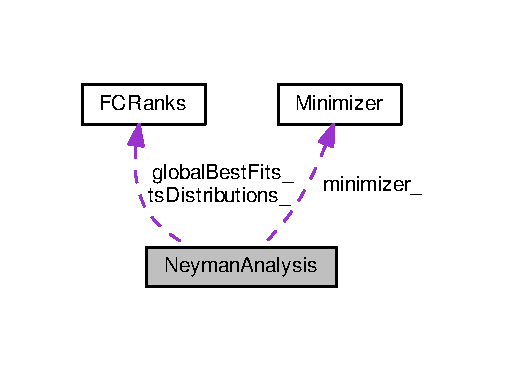
\includegraphics[width=243pt]{classNeymanAnalysis__coll__graph}
\end{center}
\end{figure}
\subsection*{Public Member Functions}
\begin{DoxyCompactItemize}
\item 
\hyperlink{classNeymanAnalysis_ab02f708099c866f0b3dabf529222846e}{Neyman\-Analysis} (boost\-::shared\-\_\-ptr$<$ \hyperlink{classLikelihood}{Likelihood} $>$ llh)
\item 
\hyperlink{classNeymanAnalysis_aa84832be2ad6a77d4570f90768ce6f12}{Neyman\-Analysis} (\hyperlink{classNeymanAnalysis}{Neyman\-Analysis} \&analysis, int64\-\_\-t seed)
\item 
double \hyperlink{classNeymanAnalysis_ab96261fccdce568c5f49c9caa3f6e585}{Evaluate\-Test\-Statistic} (double xi)
\item 
std\-::vector$<$ double $>$ \hyperlink{classNeymanAnalysis_af1382c7a6b0a799adb9b5cba89142c7e}{Test\-Statistic\-Distribution} (double xi, uint64\-\_\-t n)
\item 
void \hyperlink{classNeymanAnalysis_a850688639ff1232d73b1b99e8d1a828d}{Compute\-Ranks} (uint64\-\_\-t n\-Experiments, double min\-Xi, double max\-Xi, uint64\-\_\-t n\-Steps, uint64\-\_\-t n\-Threads, uint64\-\_\-t max\-Experiments\-Per\-Thread)
\item 
void \hyperlink{classNeymanAnalysis_a517570cbdf64019af5543cc175ce271f}{Set\-F\-C\-Ranks} (\hyperlink{classFCRanks}{F\-C\-Ranks} const \&ts\-Distributions)
\item 
void \hyperlink{classNeymanAnalysis_a48a2e22b564fcf5d001d5b397a778319}{Sample} (double xi)
\item 
std\-::vector$<$ double $>$ \hyperlink{classNeymanAnalysis_a210d3928ce874e3a1cb7667fb6c30746}{Test\-Statistic\-Distribution} (double xi)
\item 
double \hyperlink{classNeymanAnalysis_a32e7f796020e908bef11bf1b6fed9aa0}{Compute\-Limit} (double ts, double cl, double prec)
\end{DoxyCompactItemize}
\subsection*{Public Attributes}
\begin{DoxyCompactItemize}
\item 
\hyperlink{classMinimizer}{Minimizer} \hyperlink{classNeymanAnalysis_ab7b0eaaf2cb5b407f1496a745111f28e}{minimizer\-\_\-}
\item 
\hyperlink{classFCRanks}{F\-C\-Ranks} \hyperlink{classNeymanAnalysis_ab7b43994330c276c03a30dbb0e7f02cd}{ts\-Distributions\-\_\-}
\item 
\hyperlink{classFCRanks}{F\-C\-Ranks} \hyperlink{classNeymanAnalysis_a1e239edced6826a979c0e2c541060ecf}{global\-Best\-Fits\-\_\-}
\end{DoxyCompactItemize}


\subsection{Detailed Description}
class\-: \hyperlink{classNeymanAnalysis}{Neyman\-Analysis} is a class which encapsulates the Neyman analysis proceedures. 

\subsection{Constructor \& Destructor Documentation}
\hypertarget{classNeymanAnalysis_ab02f708099c866f0b3dabf529222846e}{\index{Neyman\-Analysis@{Neyman\-Analysis}!Neyman\-Analysis@{Neyman\-Analysis}}
\index{Neyman\-Analysis@{Neyman\-Analysis}!NeymanAnalysis@{Neyman\-Analysis}}
\subsubsection[{Neyman\-Analysis}]{\setlength{\rightskip}{0pt plus 5cm}Neyman\-Analysis\-::\-Neyman\-Analysis (
\begin{DoxyParamCaption}
\item[{boost\-::shared\-\_\-ptr$<$ {\bf Likelihood} $>$}]{llh}
\end{DoxyParamCaption}
)\hspace{0.3cm}{\ttfamily [inline]}}}\label{classNeymanAnalysis_ab02f708099c866f0b3dabf529222846e}
\hypertarget{classNeymanAnalysis_aa84832be2ad6a77d4570f90768ce6f12}{\index{Neyman\-Analysis@{Neyman\-Analysis}!Neyman\-Analysis@{Neyman\-Analysis}}
\index{Neyman\-Analysis@{Neyman\-Analysis}!NeymanAnalysis@{Neyman\-Analysis}}
\subsubsection[{Neyman\-Analysis}]{\setlength{\rightskip}{0pt plus 5cm}Neyman\-Analysis\-::\-Neyman\-Analysis (
\begin{DoxyParamCaption}
\item[{{\bf Neyman\-Analysis} \&}]{analysis, }
\item[{int64\-\_\-t}]{seed}
\end{DoxyParamCaption}
)}}\label{classNeymanAnalysis_aa84832be2ad6a77d4570f90768ce6f12}


\subsection{Member Function Documentation}
\hypertarget{classNeymanAnalysis_a32e7f796020e908bef11bf1b6fed9aa0}{\index{Neyman\-Analysis@{Neyman\-Analysis}!Compute\-Limit@{Compute\-Limit}}
\index{Compute\-Limit@{Compute\-Limit}!NeymanAnalysis@{Neyman\-Analysis}}
\subsubsection[{Compute\-Limit}]{\setlength{\rightskip}{0pt plus 5cm}double Neyman\-Analysis\-::\-Compute\-Limit (
\begin{DoxyParamCaption}
\item[{double}]{ts, }
\item[{double}]{cl, }
\item[{double}]{prec}
\end{DoxyParamCaption}
)}}\label{classNeymanAnalysis_a32e7f796020e908bef11bf1b6fed9aa0}
\hypertarget{classNeymanAnalysis_a850688639ff1232d73b1b99e8d1a828d}{\index{Neyman\-Analysis@{Neyman\-Analysis}!Compute\-Ranks@{Compute\-Ranks}}
\index{Compute\-Ranks@{Compute\-Ranks}!NeymanAnalysis@{Neyman\-Analysis}}
\subsubsection[{Compute\-Ranks}]{\setlength{\rightskip}{0pt plus 5cm}void Neyman\-Analysis\-::\-Compute\-Ranks (
\begin{DoxyParamCaption}
\item[{uint64\-\_\-t}]{n\-Experiments, }
\item[{double}]{min\-Xi, }
\item[{double}]{max\-Xi, }
\item[{uint64\-\_\-t}]{n\-Steps, }
\item[{uint64\-\_\-t}]{n\-Threads, }
\item[{uint64\-\_\-t}]{max\-Experiments\-Per\-Thread}
\end{DoxyParamCaption}
)}}\label{classNeymanAnalysis_a850688639ff1232d73b1b99e8d1a828d}
\hypertarget{classNeymanAnalysis_ab96261fccdce568c5f49c9caa3f6e585}{\index{Neyman\-Analysis@{Neyman\-Analysis}!Evaluate\-Test\-Statistic@{Evaluate\-Test\-Statistic}}
\index{Evaluate\-Test\-Statistic@{Evaluate\-Test\-Statistic}!NeymanAnalysis@{Neyman\-Analysis}}
\subsubsection[{Evaluate\-Test\-Statistic}]{\setlength{\rightskip}{0pt plus 5cm}double Neyman\-Analysis\-::\-Evaluate\-Test\-Statistic (
\begin{DoxyParamCaption}
\item[{double}]{xi}
\end{DoxyParamCaption}
)\hspace{0.3cm}{\ttfamily [inline]}}}\label{classNeymanAnalysis_ab96261fccdce568c5f49c9caa3f6e585}
Returns the log value of the F\-C test-\/statistic for a given likelihood parameter 
\begin{DoxyParams}{Parameters}
{\em xi} & likelihood parameter for which the test statistic should be calculated \\
\hline
\end{DoxyParams}
\begin{DoxyReturn}{Returns}
the log of the F\-C test-\/statistic = log(L(xi)/\-L(xi\-\_\-best)) 
\end{DoxyReturn}
\hypertarget{classNeymanAnalysis_a48a2e22b564fcf5d001d5b397a778319}{\index{Neyman\-Analysis@{Neyman\-Analysis}!Sample@{Sample}}
\index{Sample@{Sample}!NeymanAnalysis@{Neyman\-Analysis}}
\subsubsection[{Sample}]{\setlength{\rightskip}{0pt plus 5cm}void Neyman\-Analysis\-::\-Sample (
\begin{DoxyParamCaption}
\item[{double}]{xi}
\end{DoxyParamCaption}
)\hspace{0.3cm}{\ttfamily [inline]}}}\label{classNeymanAnalysis_a48a2e22b564fcf5d001d5b397a778319}
\hypertarget{classNeymanAnalysis_a517570cbdf64019af5543cc175ce271f}{\index{Neyman\-Analysis@{Neyman\-Analysis}!Set\-F\-C\-Ranks@{Set\-F\-C\-Ranks}}
\index{Set\-F\-C\-Ranks@{Set\-F\-C\-Ranks}!NeymanAnalysis@{Neyman\-Analysis}}
\subsubsection[{Set\-F\-C\-Ranks}]{\setlength{\rightskip}{0pt plus 5cm}void Neyman\-Analysis\-::\-Set\-F\-C\-Ranks (
\begin{DoxyParamCaption}
\item[{{\bf F\-C\-Ranks} const \&}]{ts\-Distributions}
\end{DoxyParamCaption}
)\hspace{0.3cm}{\ttfamily [inline]}}}\label{classNeymanAnalysis_a517570cbdf64019af5543cc175ce271f}
\hypertarget{classNeymanAnalysis_af1382c7a6b0a799adb9b5cba89142c7e}{\index{Neyman\-Analysis@{Neyman\-Analysis}!Test\-Statistic\-Distribution@{Test\-Statistic\-Distribution}}
\index{Test\-Statistic\-Distribution@{Test\-Statistic\-Distribution}!NeymanAnalysis@{Neyman\-Analysis}}
\subsubsection[{Test\-Statistic\-Distribution}]{\setlength{\rightskip}{0pt plus 5cm}std\-::vector$<$ double $>$ Neyman\-Analysis\-::\-Test\-Statistic\-Distribution (
\begin{DoxyParamCaption}
\item[{double}]{xi, }
\item[{uint64\-\_\-t}]{n}
\end{DoxyParamCaption}
)}}\label{classNeymanAnalysis_af1382c7a6b0a799adb9b5cba89142c7e}
\hypertarget{classNeymanAnalysis_a210d3928ce874e3a1cb7667fb6c30746}{\index{Neyman\-Analysis@{Neyman\-Analysis}!Test\-Statistic\-Distribution@{Test\-Statistic\-Distribution}}
\index{Test\-Statistic\-Distribution@{Test\-Statistic\-Distribution}!NeymanAnalysis@{Neyman\-Analysis}}
\subsubsection[{Test\-Statistic\-Distribution}]{\setlength{\rightskip}{0pt plus 5cm}std\-::vector$<$double$>$ Neyman\-Analysis\-::\-Test\-Statistic\-Distribution (
\begin{DoxyParamCaption}
\item[{double}]{xi}
\end{DoxyParamCaption}
)}}\label{classNeymanAnalysis_a210d3928ce874e3a1cb7667fb6c30746}


\subsection{Member Data Documentation}
\hypertarget{classNeymanAnalysis_a1e239edced6826a979c0e2c541060ecf}{\index{Neyman\-Analysis@{Neyman\-Analysis}!global\-Best\-Fits\-\_\-@{global\-Best\-Fits\-\_\-}}
\index{global\-Best\-Fits\-\_\-@{global\-Best\-Fits\-\_\-}!NeymanAnalysis@{Neyman\-Analysis}}
\subsubsection[{global\-Best\-Fits\-\_\-}]{\setlength{\rightskip}{0pt plus 5cm}{\bf F\-C\-Ranks} Neyman\-Analysis\-::global\-Best\-Fits\-\_\-}}\label{classNeymanAnalysis_a1e239edced6826a979c0e2c541060ecf}
\hypertarget{classNeymanAnalysis_ab7b0eaaf2cb5b407f1496a745111f28e}{\index{Neyman\-Analysis@{Neyman\-Analysis}!minimizer\-\_\-@{minimizer\-\_\-}}
\index{minimizer\-\_\-@{minimizer\-\_\-}!NeymanAnalysis@{Neyman\-Analysis}}
\subsubsection[{minimizer\-\_\-}]{\setlength{\rightskip}{0pt plus 5cm}{\bf Minimizer} Neyman\-Analysis\-::minimizer\-\_\-}}\label{classNeymanAnalysis_ab7b0eaaf2cb5b407f1496a745111f28e}
\hypertarget{classNeymanAnalysis_ab7b43994330c276c03a30dbb0e7f02cd}{\index{Neyman\-Analysis@{Neyman\-Analysis}!ts\-Distributions\-\_\-@{ts\-Distributions\-\_\-}}
\index{ts\-Distributions\-\_\-@{ts\-Distributions\-\_\-}!NeymanAnalysis@{Neyman\-Analysis}}
\subsubsection[{ts\-Distributions\-\_\-}]{\setlength{\rightskip}{0pt plus 5cm}{\bf F\-C\-Ranks} Neyman\-Analysis\-::ts\-Distributions\-\_\-}}\label{classNeymanAnalysis_ab7b43994330c276c03a30dbb0e7f02cd}


The documentation for this class was generated from the following files\-:\begin{DoxyCompactItemize}
\item 
/home/travis/build/sflis/\-M\-L\-Sandbox/public/\-M\-L\-Sandbox/\hyperlink{NeymanAnalysis_8h}{Neyman\-Analysis.\-h}\item 
/home/travis/build/sflis/\-M\-L\-Sandbox/private/\-M\-L\-Sandbox/\hyperlink{MLSandbox_2NeymanAnalysis_8cxx}{Neyman\-Analysis.\-cxx}\end{DoxyCompactItemize}

\hypertarget{structNeymanThreadData}{\section{Neyman\-Thread\-Data Struct Reference}
\label{structNeymanThreadData}\index{Neyman\-Thread\-Data@{Neyman\-Thread\-Data}}
}


Collaboration diagram for Neyman\-Thread\-Data\-:
\nopagebreak
\begin{figure}[H]
\begin{center}
\leavevmode
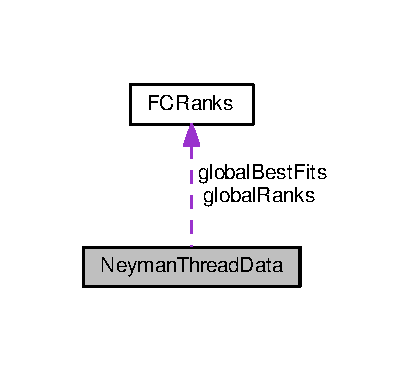
\includegraphics[width=198pt]{structNeymanThreadData__coll__graph}
\end{center}
\end{figure}
\subsection*{Public Member Functions}
\begin{DoxyCompactItemize}
\item 
\hyperlink{structNeymanThreadData_a25be57cca6f0dd8fd3a5d0e5525a35c4}{Neyman\-Thread\-Data} (boost\-::shared\-\_\-ptr$<$ \hyperlink{classNeymanAnalysis}{Neyman\-Analysis} $>$ \hyperlink{structNeymanThreadData_a4b9b47c80fd8fa5ea300485a923f2348}{ana}, \hyperlink{classFCRanks}{F\-C\-Ranks} \&\hyperlink{structNeymanThreadData_a800f5dd68444c0ec9654946105759afc}{global\-Ranks}, \hyperlink{classFCRanks}{F\-C\-Ranks} \&\hyperlink{structNeymanThreadData_a5de558380b8e1c7c08960526d91d8841}{global\-Best\-Fits}, std\-::queue$<$ \hyperlink{structjob}{job} $>$ \&\hyperlink{structNeymanThreadData_ad7e388c9438a16640110fbe9018fda90}{job\-Queue}, uint64\-\_\-t \hyperlink{structNeymanThreadData_a99154b06d67a82c8bf48112beabbd7ec}{n\-Experiments}, uint64\-\_\-t \hyperlink{structNeymanThreadData_a0d26db26796419914c2a9a35214a26b3}{thread\-Number}, double \hyperlink{structNeymanThreadData_af145feca7df9e9c5c88bec759d97ba8f}{cl}, uint64\-\_\-t n\-Hypotheses, uint64\-\_\-t \&\hyperlink{structNeymanThreadData_acab7f8af86761370c3bb06132b0e92f5}{n\-Tested\-Hypotheses})
\end{DoxyCompactItemize}
\subsection*{Public Attributes}
\begin{DoxyCompactItemize}
\item 
boost\-::shared\-\_\-ptr$<$ \hyperlink{classNeymanAnalysis}{Neyman\-Analysis} $>$ \hyperlink{structNeymanThreadData_a4b9b47c80fd8fa5ea300485a923f2348}{ana}
\item 
\hyperlink{classFCRanks}{F\-C\-Ranks} \& \hyperlink{structNeymanThreadData_a800f5dd68444c0ec9654946105759afc}{global\-Ranks}
\item 
\hyperlink{classFCRanks}{F\-C\-Ranks} \& \hyperlink{structNeymanThreadData_a5de558380b8e1c7c08960526d91d8841}{global\-Best\-Fits}
\item 
std\-::queue$<$ \hyperlink{structjob}{job} $>$ \& \hyperlink{structNeymanThreadData_ad7e388c9438a16640110fbe9018fda90}{job\-Queue}
\item 
uint64\-\_\-t \hyperlink{structNeymanThreadData_a99154b06d67a82c8bf48112beabbd7ec}{n\-Experiments}
\item 
uint64\-\_\-t \hyperlink{structNeymanThreadData_a0d26db26796419914c2a9a35214a26b3}{thread\-Number}
\item 
double \hyperlink{structNeymanThreadData_af145feca7df9e9c5c88bec759d97ba8f}{cl}
\item 
uint64\-\_\-t \hyperlink{structNeymanThreadData_a129c6ff7d2f1d5102fa6543ff0683d1b}{total\-Hypotheses}
\item 
uint64\-\_\-t \& \hyperlink{structNeymanThreadData_acab7f8af86761370c3bb06132b0e92f5}{n\-Tested\-Hypotheses}
\end{DoxyCompactItemize}


\subsection{Constructor \& Destructor Documentation}
\hypertarget{structNeymanThreadData_a25be57cca6f0dd8fd3a5d0e5525a35c4}{\index{Neyman\-Thread\-Data@{Neyman\-Thread\-Data}!Neyman\-Thread\-Data@{Neyman\-Thread\-Data}}
\index{Neyman\-Thread\-Data@{Neyman\-Thread\-Data}!NeymanThreadData@{Neyman\-Thread\-Data}}
\subsubsection[{Neyman\-Thread\-Data}]{\setlength{\rightskip}{0pt plus 5cm}Neyman\-Thread\-Data\-::\-Neyman\-Thread\-Data (
\begin{DoxyParamCaption}
\item[{boost\-::shared\-\_\-ptr$<$ {\bf Neyman\-Analysis} $>$}]{ana, }
\item[{{\bf F\-C\-Ranks} \&}]{global\-Ranks, }
\item[{{\bf F\-C\-Ranks} \&}]{global\-Best\-Fits, }
\item[{std\-::queue$<$ {\bf job} $>$ \&}]{job\-Queue, }
\item[{uint64\-\_\-t}]{n\-Experiments, }
\item[{uint64\-\_\-t}]{thread\-Number, }
\item[{double}]{cl, }
\item[{uint64\-\_\-t}]{n\-Hypotheses, }
\item[{uint64\-\_\-t \&}]{n\-Tested\-Hypotheses}
\end{DoxyParamCaption}
)\hspace{0.3cm}{\ttfamily [inline]}}}\label{structNeymanThreadData_a25be57cca6f0dd8fd3a5d0e5525a35c4}


\subsection{Member Data Documentation}
\hypertarget{structNeymanThreadData_a4b9b47c80fd8fa5ea300485a923f2348}{\index{Neyman\-Thread\-Data@{Neyman\-Thread\-Data}!ana@{ana}}
\index{ana@{ana}!NeymanThreadData@{Neyman\-Thread\-Data}}
\subsubsection[{ana}]{\setlength{\rightskip}{0pt plus 5cm}boost\-::shared\-\_\-ptr$<${\bf Neyman\-Analysis}$>$ Neyman\-Thread\-Data\-::ana}}\label{structNeymanThreadData_a4b9b47c80fd8fa5ea300485a923f2348}
\hypertarget{structNeymanThreadData_af145feca7df9e9c5c88bec759d97ba8f}{\index{Neyman\-Thread\-Data@{Neyman\-Thread\-Data}!cl@{cl}}
\index{cl@{cl}!NeymanThreadData@{Neyman\-Thread\-Data}}
\subsubsection[{cl}]{\setlength{\rightskip}{0pt plus 5cm}double Neyman\-Thread\-Data\-::cl}}\label{structNeymanThreadData_af145feca7df9e9c5c88bec759d97ba8f}
\hypertarget{structNeymanThreadData_a5de558380b8e1c7c08960526d91d8841}{\index{Neyman\-Thread\-Data@{Neyman\-Thread\-Data}!global\-Best\-Fits@{global\-Best\-Fits}}
\index{global\-Best\-Fits@{global\-Best\-Fits}!NeymanThreadData@{Neyman\-Thread\-Data}}
\subsubsection[{global\-Best\-Fits}]{\setlength{\rightskip}{0pt plus 5cm}{\bf F\-C\-Ranks}\& Neyman\-Thread\-Data\-::global\-Best\-Fits}}\label{structNeymanThreadData_a5de558380b8e1c7c08960526d91d8841}
\hypertarget{structNeymanThreadData_a800f5dd68444c0ec9654946105759afc}{\index{Neyman\-Thread\-Data@{Neyman\-Thread\-Data}!global\-Ranks@{global\-Ranks}}
\index{global\-Ranks@{global\-Ranks}!NeymanThreadData@{Neyman\-Thread\-Data}}
\subsubsection[{global\-Ranks}]{\setlength{\rightskip}{0pt plus 5cm}{\bf F\-C\-Ranks}\& Neyman\-Thread\-Data\-::global\-Ranks}}\label{structNeymanThreadData_a800f5dd68444c0ec9654946105759afc}
\hypertarget{structNeymanThreadData_ad7e388c9438a16640110fbe9018fda90}{\index{Neyman\-Thread\-Data@{Neyman\-Thread\-Data}!job\-Queue@{job\-Queue}}
\index{job\-Queue@{job\-Queue}!NeymanThreadData@{Neyman\-Thread\-Data}}
\subsubsection[{job\-Queue}]{\setlength{\rightskip}{0pt plus 5cm}std\-::queue$<${\bf job}$>$\& Neyman\-Thread\-Data\-::job\-Queue}}\label{structNeymanThreadData_ad7e388c9438a16640110fbe9018fda90}
\hypertarget{structNeymanThreadData_a99154b06d67a82c8bf48112beabbd7ec}{\index{Neyman\-Thread\-Data@{Neyman\-Thread\-Data}!n\-Experiments@{n\-Experiments}}
\index{n\-Experiments@{n\-Experiments}!NeymanThreadData@{Neyman\-Thread\-Data}}
\subsubsection[{n\-Experiments}]{\setlength{\rightskip}{0pt plus 5cm}uint64\-\_\-t Neyman\-Thread\-Data\-::n\-Experiments}}\label{structNeymanThreadData_a99154b06d67a82c8bf48112beabbd7ec}
\hypertarget{structNeymanThreadData_acab7f8af86761370c3bb06132b0e92f5}{\index{Neyman\-Thread\-Data@{Neyman\-Thread\-Data}!n\-Tested\-Hypotheses@{n\-Tested\-Hypotheses}}
\index{n\-Tested\-Hypotheses@{n\-Tested\-Hypotheses}!NeymanThreadData@{Neyman\-Thread\-Data}}
\subsubsection[{n\-Tested\-Hypotheses}]{\setlength{\rightskip}{0pt plus 5cm}uint64\-\_\-t\& Neyman\-Thread\-Data\-::n\-Tested\-Hypotheses}}\label{structNeymanThreadData_acab7f8af86761370c3bb06132b0e92f5}
\hypertarget{structNeymanThreadData_a0d26db26796419914c2a9a35214a26b3}{\index{Neyman\-Thread\-Data@{Neyman\-Thread\-Data}!thread\-Number@{thread\-Number}}
\index{thread\-Number@{thread\-Number}!NeymanThreadData@{Neyman\-Thread\-Data}}
\subsubsection[{thread\-Number}]{\setlength{\rightskip}{0pt plus 5cm}uint64\-\_\-t Neyman\-Thread\-Data\-::thread\-Number}}\label{structNeymanThreadData_a0d26db26796419914c2a9a35214a26b3}
\hypertarget{structNeymanThreadData_a129c6ff7d2f1d5102fa6543ff0683d1b}{\index{Neyman\-Thread\-Data@{Neyman\-Thread\-Data}!total\-Hypotheses@{total\-Hypotheses}}
\index{total\-Hypotheses@{total\-Hypotheses}!NeymanThreadData@{Neyman\-Thread\-Data}}
\subsubsection[{total\-Hypotheses}]{\setlength{\rightskip}{0pt plus 5cm}uint64\-\_\-t Neyman\-Thread\-Data\-::total\-Hypotheses}}\label{structNeymanThreadData_a129c6ff7d2f1d5102fa6543ff0683d1b}


The documentation for this struct was generated from the following file\-:\begin{DoxyCompactItemize}
\item 
/home/travis/build/sflis/\-M\-L\-Sandbox/private/\-M\-L\-Sandbox/\hyperlink{MLSandbox_2NeymanAnalysis_8cxx}{Neyman\-Analysis.\-cxx}\end{DoxyCompactItemize}

\hypertarget{classRNG}{\section{R\-N\-G Class Reference}
\label{classRNG}\index{R\-N\-G@{R\-N\-G}}
}


A small wrapper class around the G\-S\-L random number generator.  




{\ttfamily \#include $<$R\-N\-G.\-h$>$}

\subsection*{Public Member Functions}
\begin{DoxyCompactItemize}
\item 
\hyperlink{classRNG_ad1a0404ddd79895cfc05432f06c9c385}{R\-N\-G} (unsigned int seed)
\item 
\hyperlink{classRNG_abe0c541fcfa0b12ef7446eccb166d510}{$\sim$\-R\-N\-G} ()
\item 
double \hyperlink{classRNG_a6f369de914cf763da0a0bc8c17affb12}{Uniform} ()
\item 
double \hyperlink{classRNG_aa8a14d0a3367ada957ab898ff6974957}{Exp} (double tau)
\item 
double \hyperlink{classRNG_a959d86ea22fc5bb2f5ff6ded9881137a}{Poisson} (double nu)
\item 
double \hyperlink{classRNG_afe51d6c541a71af3a80c2ecf86d81523}{Gauss} (double mu, double sigma)
\item 
double \hyperlink{classRNG_a37fc5d27bda97b756e92565183f48d66}{Binomial} (double p, double N)
\end{DoxyCompactItemize}
\subsection*{Public Attributes}
\begin{DoxyCompactItemize}
\item 
unsigned int \hyperlink{classRNG_aa644a44fe1386322507d92e23066d063}{seed\-\_\-}
\end{DoxyCompactItemize}


\subsection{Detailed Description}
A small wrapper class around the G\-S\-L random number generator. 

class\-: \hyperlink{classRNG}{R\-N\-G} 

\subsection{Constructor \& Destructor Documentation}
\hypertarget{classRNG_ad1a0404ddd79895cfc05432f06c9c385}{\index{R\-N\-G@{R\-N\-G}!R\-N\-G@{R\-N\-G}}
\index{R\-N\-G@{R\-N\-G}!RNG@{R\-N\-G}}
\subsubsection[{R\-N\-G}]{\setlength{\rightskip}{0pt plus 5cm}R\-N\-G\-::\-R\-N\-G (
\begin{DoxyParamCaption}
\item[{unsigned int}]{seed}
\end{DoxyParamCaption}
)\hspace{0.3cm}{\ttfamily [inline]}}}\label{classRNG_ad1a0404ddd79895cfc05432f06c9c385}
\hypertarget{classRNG_abe0c541fcfa0b12ef7446eccb166d510}{\index{R\-N\-G@{R\-N\-G}!$\sim$\-R\-N\-G@{$\sim$\-R\-N\-G}}
\index{$\sim$\-R\-N\-G@{$\sim$\-R\-N\-G}!RNG@{R\-N\-G}}
\subsubsection[{$\sim$\-R\-N\-G}]{\setlength{\rightskip}{0pt plus 5cm}R\-N\-G\-::$\sim$\-R\-N\-G (
\begin{DoxyParamCaption}
{}
\end{DoxyParamCaption}
)\hspace{0.3cm}{\ttfamily [inline]}}}\label{classRNG_abe0c541fcfa0b12ef7446eccb166d510}


\subsection{Member Function Documentation}
\hypertarget{classRNG_a37fc5d27bda97b756e92565183f48d66}{\index{R\-N\-G@{R\-N\-G}!Binomial@{Binomial}}
\index{Binomial@{Binomial}!RNG@{R\-N\-G}}
\subsubsection[{Binomial}]{\setlength{\rightskip}{0pt plus 5cm}double R\-N\-G\-::\-Binomial (
\begin{DoxyParamCaption}
\item[{double}]{p, }
\item[{double}]{N}
\end{DoxyParamCaption}
)\hspace{0.3cm}{\ttfamily [inline]}}}\label{classRNG_a37fc5d27bda97b756e92565183f48d66}
\hypertarget{classRNG_aa8a14d0a3367ada957ab898ff6974957}{\index{R\-N\-G@{R\-N\-G}!Exp@{Exp}}
\index{Exp@{Exp}!RNG@{R\-N\-G}}
\subsubsection[{Exp}]{\setlength{\rightskip}{0pt plus 5cm}double R\-N\-G\-::\-Exp (
\begin{DoxyParamCaption}
\item[{double}]{tau}
\end{DoxyParamCaption}
)\hspace{0.3cm}{\ttfamily [inline]}}}\label{classRNG_aa8a14d0a3367ada957ab898ff6974957}
\hypertarget{classRNG_afe51d6c541a71af3a80c2ecf86d81523}{\index{R\-N\-G@{R\-N\-G}!Gauss@{Gauss}}
\index{Gauss@{Gauss}!RNG@{R\-N\-G}}
\subsubsection[{Gauss}]{\setlength{\rightskip}{0pt plus 5cm}double R\-N\-G\-::\-Gauss (
\begin{DoxyParamCaption}
\item[{double}]{mu, }
\item[{double}]{sigma}
\end{DoxyParamCaption}
)\hspace{0.3cm}{\ttfamily [inline]}}}\label{classRNG_afe51d6c541a71af3a80c2ecf86d81523}
\hypertarget{classRNG_a959d86ea22fc5bb2f5ff6ded9881137a}{\index{R\-N\-G@{R\-N\-G}!Poisson@{Poisson}}
\index{Poisson@{Poisson}!RNG@{R\-N\-G}}
\subsubsection[{Poisson}]{\setlength{\rightskip}{0pt plus 5cm}double R\-N\-G\-::\-Poisson (
\begin{DoxyParamCaption}
\item[{double}]{nu}
\end{DoxyParamCaption}
)\hspace{0.3cm}{\ttfamily [inline]}}}\label{classRNG_a959d86ea22fc5bb2f5ff6ded9881137a}
\hypertarget{classRNG_a6f369de914cf763da0a0bc8c17affb12}{\index{R\-N\-G@{R\-N\-G}!Uniform@{Uniform}}
\index{Uniform@{Uniform}!RNG@{R\-N\-G}}
\subsubsection[{Uniform}]{\setlength{\rightskip}{0pt plus 5cm}double R\-N\-G\-::\-Uniform (
\begin{DoxyParamCaption}
{}
\end{DoxyParamCaption}
)\hspace{0.3cm}{\ttfamily [inline]}}}\label{classRNG_a6f369de914cf763da0a0bc8c17affb12}


\subsection{Member Data Documentation}
\hypertarget{classRNG_aa644a44fe1386322507d92e23066d063}{\index{R\-N\-G@{R\-N\-G}!seed\-\_\-@{seed\-\_\-}}
\index{seed\-\_\-@{seed\-\_\-}!RNG@{R\-N\-G}}
\subsubsection[{seed\-\_\-}]{\setlength{\rightskip}{0pt plus 5cm}unsigned int R\-N\-G\-::seed\-\_\-}}\label{classRNG_aa644a44fe1386322507d92e23066d063}


The documentation for this class was generated from the following file\-:\begin{DoxyCompactItemize}
\item 
/home/travis/build/sflis/\-M\-L\-Sandbox/public/\-M\-L\-Sandbox/\hyperlink{RNG_8h}{R\-N\-G.\-h}\end{DoxyCompactItemize}

\hypertarget{classShapeLikelihood}{\section{Shape\-Likelihood Class Reference}
\label{classShapeLikelihood}\index{Shape\-Likelihood@{Shape\-Likelihood}}
}


A class that provides functions to compute a 1 dimensional \hyperlink{classLikelihood}{Likelihood} of the form\-: \[ L(\xi) = \prod^N_{k=1} (\xi f_{sig}(x_k) + (1-\xi) f_{bg}(x_k)) \].  




{\ttfamily \#include $<$Likelihood.\-h$>$}



Inheritance diagram for Shape\-Likelihood\-:
\nopagebreak
\begin{figure}[H]
\begin{center}
\leavevmode
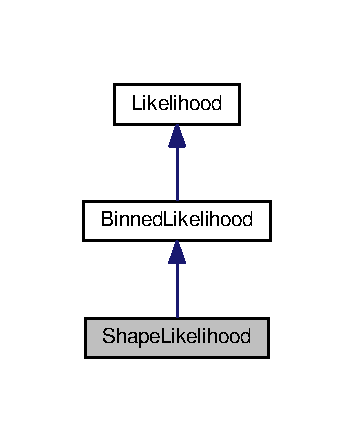
\includegraphics[width=170pt]{classShapeLikelihood__inherit__graph}
\end{center}
\end{figure}


Collaboration diagram for Shape\-Likelihood\-:
\nopagebreak
\begin{figure}[H]
\begin{center}
\leavevmode
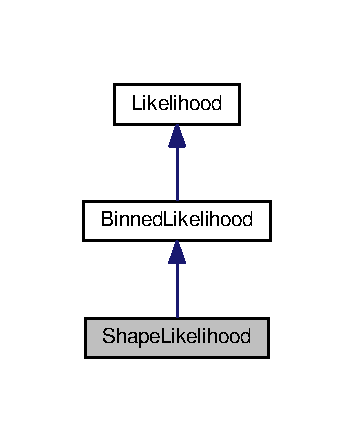
\includegraphics[width=170pt]{classShapeLikelihood__coll__graph}
\end{center}
\end{figure}
\subsection*{Public Member Functions}
\begin{DoxyCompactItemize}
\item 
\hyperlink{classShapeLikelihood_aa55ad8f50f5965c942efcdf6bff59713}{Shape\-Likelihood} (const \hyperlink{classDistribution}{Distribution} \&signal, const \hyperlink{classDistribution}{Distribution} \&background, const \hyperlink{classDistribution}{Distribution} \&signal\-Sample, const \hyperlink{classDistribution}{Distribution} \&background\-Sample, double N, bool histograming=false, bool poisson\-Sampling=false, int seed=1)
\item 
\hyperlink{classShapeLikelihood_a138035dc74b7e1cb135e93afaf9e56d7}{Shape\-Likelihood} (const \hyperlink{classDistribution}{Distribution} \&signal, const \hyperlink{classDistribution}{Distribution} \&background, const \hyperlink{classDistribution}{Distribution} \&signal\-Sample, const \hyperlink{classDistribution}{Distribution} \&background\-Sample, double N, int seed=1)
\item 
double \hyperlink{classShapeLikelihood_afe024bedaab4633ded018d23d17c37f8}{Evaluate\-L\-L\-H} (double xi) const 
\item 
void \hyperlink{classShapeLikelihood_aa303861500c399cb680d89b15d08b806}{Sample\-Events} (double xi)
\begin{DoxyCompactList}\small\item\em Generates a new observation (event sample) based on the sampling pdfs. \end{DoxyCompactList}\item 
\hyperlink{Likelihood_8h_a97d92c5c141f28319e7e8198defc9084}{likelihood\-Callback} \hyperlink{classShapeLikelihood_acf56e312fd4f0881aa09215d73b93412}{Call\-Back\-Fcn} ()
\begin{DoxyCompactList}\small\item\em A callback function of the likelihood evaluation to be passed to the minimizer. \end{DoxyCompactList}\item 
void \hyperlink{classShapeLikelihood_aad505df9d12960a6ed614f8c56b87b16}{Enable\-Poisson\-Sampling} ()
\item 
double \hyperlink{classShapeLikelihood_a03f18beacb939bb6766c93e1a9d202b4}{Xi2\-Mu} (double xi) const 
\item 
double \hyperlink{classShapeLikelihood_a37d2b69c8d222ffccd0a649f91272043}{Mu2\-Xi} (double mu) const 
\item 
\hyperlink{classShapeLikelihood}{Shape\-Likelihood} $\ast$ \hyperlink{classShapeLikelihood_a67630eb790d07ef1d0d2e33711495cbe}{Clone} (int seed) const 
\end{DoxyCompactItemize}
\subsection*{Additional Inherited Members}


\subsection{Detailed Description}
A class that provides functions to compute a 1 dimensional \hyperlink{classLikelihood}{Likelihood} of the form\-: \[ L(\xi) = \prod^N_{k=1} (\xi f_{sig}(x_k) + (1-\xi) f_{bg}(x_k)) \]. 

class\-: \hyperlink{classShapeLikelihood}{Shape\-Likelihood} Table containing abbreviations used for variables and explenations in the comments\-: \par
 N\-: number of observed events \par
 xi = $ \xi = \mu / N $\-: signal fraction \par
 x\-: pdf observable \par


\subsection{Constructor \& Destructor Documentation}
\hypertarget{classShapeLikelihood_aa55ad8f50f5965c942efcdf6bff59713}{\index{Shape\-Likelihood@{Shape\-Likelihood}!Shape\-Likelihood@{Shape\-Likelihood}}
\index{Shape\-Likelihood@{Shape\-Likelihood}!ShapeLikelihood@{Shape\-Likelihood}}
\subsubsection[{Shape\-Likelihood}]{\setlength{\rightskip}{0pt plus 5cm}Shape\-Likelihood\-::\-Shape\-Likelihood (
\begin{DoxyParamCaption}
\item[{const {\bf Distribution} \&}]{signal, }
\item[{const {\bf Distribution} \&}]{background, }
\item[{const {\bf Distribution} \&}]{signal\-Sample, }
\item[{const {\bf Distribution} \&}]{background\-Sample, }
\item[{double}]{N, }
\item[{bool}]{histograming = {\ttfamily false}, }
\item[{bool}]{poisson\-Sampling = {\ttfamily false}, }
\item[{int}]{seed = {\ttfamily 1}}
\end{DoxyParamCaption}
)\hspace{0.3cm}{\ttfamily [inline]}}}\label{classShapeLikelihood_aa55ad8f50f5965c942efcdf6bff59713}
The Simple\-Shape\-Likelihood constructor 
\begin{DoxyParams}{Parameters}
{\em signal} & signal expectation (pdf) \\
\hline
{\em background} & background expectation (pdf) \\
\hline
{\em signal\-Sample} & \\
\hline
{\em background} & \\
\hline
{\em N} & number of events in sample \\
\hline
{\em seed} & random number generator seed \\
\hline
\end{DoxyParams}
\hypertarget{classShapeLikelihood_a138035dc74b7e1cb135e93afaf9e56d7}{\index{Shape\-Likelihood@{Shape\-Likelihood}!Shape\-Likelihood@{Shape\-Likelihood}}
\index{Shape\-Likelihood@{Shape\-Likelihood}!ShapeLikelihood@{Shape\-Likelihood}}
\subsubsection[{Shape\-Likelihood}]{\setlength{\rightskip}{0pt plus 5cm}Shape\-Likelihood\-::\-Shape\-Likelihood (
\begin{DoxyParamCaption}
\item[{const {\bf Distribution} \&}]{signal, }
\item[{const {\bf Distribution} \&}]{background, }
\item[{const {\bf Distribution} \&}]{signal\-Sample, }
\item[{const {\bf Distribution} \&}]{background\-Sample, }
\item[{double}]{N, }
\item[{int}]{seed = {\ttfamily 1}}
\end{DoxyParamCaption}
)\hspace{0.3cm}{\ttfamily [inline]}}}\label{classShapeLikelihood_a138035dc74b7e1cb135e93afaf9e56d7}
The Simple\-Shape\-Likelihood constructor 
\begin{DoxyParams}{Parameters}
{\em signal} & signal expectation (pdf) \\
\hline
{\em background} & background expectation (pdf) \\
\hline
{\em signal\-Sample} & \\
\hline
{\em background} & \\
\hline
{\em N} & number of events in sample \\
\hline
{\em seed} & random number generator seed \\
\hline
\end{DoxyParams}


\subsection{Member Function Documentation}
\hypertarget{classShapeLikelihood_acf56e312fd4f0881aa09215d73b93412}{\index{Shape\-Likelihood@{Shape\-Likelihood}!Call\-Back\-Fcn@{Call\-Back\-Fcn}}
\index{Call\-Back\-Fcn@{Call\-Back\-Fcn}!ShapeLikelihood@{Shape\-Likelihood}}
\subsubsection[{Call\-Back\-Fcn}]{\setlength{\rightskip}{0pt plus 5cm}{\bf likelihood\-Callback} Shape\-Likelihood\-::\-Call\-Back\-Fcn (
\begin{DoxyParamCaption}
{}
\end{DoxyParamCaption}
)\hspace{0.3cm}{\ttfamily [inline]}, {\ttfamily [virtual]}}}\label{classShapeLikelihood_acf56e312fd4f0881aa09215d73b93412}


A callback function of the likelihood evaluation to be passed to the minimizer. 



Implements \hyperlink{classBinnedLikelihood_aed7e05d58a36f515afc8e34fe8550b31}{Binned\-Likelihood}.

\hypertarget{classShapeLikelihood_a67630eb790d07ef1d0d2e33711495cbe}{\index{Shape\-Likelihood@{Shape\-Likelihood}!Clone@{Clone}}
\index{Clone@{Clone}!ShapeLikelihood@{Shape\-Likelihood}}
\subsubsection[{Clone}]{\setlength{\rightskip}{0pt plus 5cm}{\bf Shape\-Likelihood}$\ast$ Shape\-Likelihood\-::\-Clone (
\begin{DoxyParamCaption}
\item[{int}]{seed}
\end{DoxyParamCaption}
) const\hspace{0.3cm}{\ttfamily [inline]}, {\ttfamily [virtual]}}}\label{classShapeLikelihood_a67630eb790d07ef1d0d2e33711495cbe}
Returns a clone of the likelihood with a possible exception of the rng seed 

Implements \hyperlink{classLikelihood_a938b362a171c46f447cb364effc83bcf}{Likelihood}.

\hypertarget{classShapeLikelihood_aad505df9d12960a6ed614f8c56b87b16}{\index{Shape\-Likelihood@{Shape\-Likelihood}!Enable\-Poisson\-Sampling@{Enable\-Poisson\-Sampling}}
\index{Enable\-Poisson\-Sampling@{Enable\-Poisson\-Sampling}!ShapeLikelihood@{Shape\-Likelihood}}
\subsubsection[{Enable\-Poisson\-Sampling}]{\setlength{\rightskip}{0pt plus 5cm}void Shape\-Likelihood\-::\-Enable\-Poisson\-Sampling (
\begin{DoxyParamCaption}
{}
\end{DoxyParamCaption}
)\hspace{0.3cm}{\ttfamily [inline]}}}\label{classShapeLikelihood_aad505df9d12960a6ed614f8c56b87b16}
\hypertarget{classShapeLikelihood_afe024bedaab4633ded018d23d17c37f8}{\index{Shape\-Likelihood@{Shape\-Likelihood}!Evaluate\-L\-L\-H@{Evaluate\-L\-L\-H}}
\index{Evaluate\-L\-L\-H@{Evaluate\-L\-L\-H}!ShapeLikelihood@{Shape\-Likelihood}}
\subsubsection[{Evaluate\-L\-L\-H}]{\setlength{\rightskip}{0pt plus 5cm}double Shape\-Likelihood\-::\-Evaluate\-L\-L\-H (
\begin{DoxyParamCaption}
\item[{double}]{xi}
\end{DoxyParamCaption}
) const\hspace{0.3cm}{\ttfamily [virtual]}}}\label{classShapeLikelihood_afe024bedaab4633ded018d23d17c37f8}
Evaluates the log likelihood sum 
\begin{DoxyParams}{Parameters}
{\em xi} & the signal fraction for which the likelihood should be evaulated. \\
\hline
\end{DoxyParams}


Implements \hyperlink{classBinnedLikelihood_a2084a64cd8b5d6bf8055538a0f633785}{Binned\-Likelihood}.

\hypertarget{classShapeLikelihood_a37d2b69c8d222ffccd0a649f91272043}{\index{Shape\-Likelihood@{Shape\-Likelihood}!Mu2\-Xi@{Mu2\-Xi}}
\index{Mu2\-Xi@{Mu2\-Xi}!ShapeLikelihood@{Shape\-Likelihood}}
\subsubsection[{Mu2\-Xi}]{\setlength{\rightskip}{0pt plus 5cm}double Shape\-Likelihood\-::\-Mu2\-Xi (
\begin{DoxyParamCaption}
\item[{double}]{mu}
\end{DoxyParamCaption}
) const\hspace{0.3cm}{\ttfamily [inline]}}}\label{classShapeLikelihood_a37d2b69c8d222ffccd0a649f91272043}
Number of signal events to signal fraction 
\begin{DoxyParams}{Parameters}
{\em mu} & number of signal events \\
\hline
\end{DoxyParams}
\begin{DoxyReturn}{Returns}
signal fraction 
\end{DoxyReturn}
\hypertarget{classShapeLikelihood_aa303861500c399cb680d89b15d08b806}{\index{Shape\-Likelihood@{Shape\-Likelihood}!Sample\-Events@{Sample\-Events}}
\index{Sample\-Events@{Sample\-Events}!ShapeLikelihood@{Shape\-Likelihood}}
\subsubsection[{Sample\-Events}]{\setlength{\rightskip}{0pt plus 5cm}void Shape\-Likelihood\-::\-Sample\-Events (
\begin{DoxyParamCaption}
\item[{double}]{xi}
\end{DoxyParamCaption}
)\hspace{0.3cm}{\ttfamily [virtual]}}}\label{classShapeLikelihood_aa303861500c399cb680d89b15d08b806}


Generates a new observation (event sample) based on the sampling pdfs. 



Implements \hyperlink{classBinnedLikelihood_a0793b8109912c6e509470a14a58d2a2a}{Binned\-Likelihood}.

\hypertarget{classShapeLikelihood_a03f18beacb939bb6766c93e1a9d202b4}{\index{Shape\-Likelihood@{Shape\-Likelihood}!Xi2\-Mu@{Xi2\-Mu}}
\index{Xi2\-Mu@{Xi2\-Mu}!ShapeLikelihood@{Shape\-Likelihood}}
\subsubsection[{Xi2\-Mu}]{\setlength{\rightskip}{0pt plus 5cm}double Shape\-Likelihood\-::\-Xi2\-Mu (
\begin{DoxyParamCaption}
\item[{double}]{xi}
\end{DoxyParamCaption}
) const\hspace{0.3cm}{\ttfamily [inline]}}}\label{classShapeLikelihood_a03f18beacb939bb6766c93e1a9d202b4}
Signal fraction to number of events 
\begin{DoxyParams}{Parameters}
{\em xi} & signal fraction \\
\hline
\end{DoxyParams}
\begin{DoxyReturn}{Returns}
number of events 
\end{DoxyReturn}


The documentation for this class was generated from the following files\-:\begin{DoxyCompactItemize}
\item 
/home/travis/build/sflis/\-M\-L\-Sandbox/public/\-M\-L\-Sandbox/\hyperlink{Likelihood_8h}{Likelihood.\-h}\item 
/home/travis/build/sflis/\-M\-L\-Sandbox/private/\-M\-L\-Sandbox/\hyperlink{MLSandbox_2Likelihood_8cxx}{Likelihood.\-cxx}\end{DoxyCompactItemize}

\hypertarget{classSignalContaminatedLH}{\section{Signal\-Contaminated\-L\-H Class Reference}
\label{classSignalContaminatedLH}\index{Signal\-Contaminated\-L\-H@{Signal\-Contaminated\-L\-H}}
}


{\ttfamily \#include $<$Signal\-Contaminated\-L\-H.\-h$>$}



Inheritance diagram for Signal\-Contaminated\-L\-H\-:
\nopagebreak
\begin{figure}[H]
\begin{center}
\leavevmode
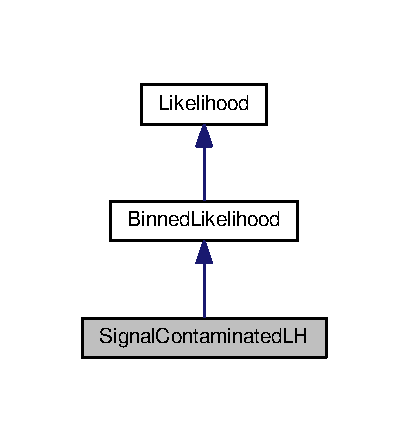
\includegraphics[width=196pt]{classSignalContaminatedLH__inherit__graph}
\end{center}
\end{figure}


Collaboration diagram for Signal\-Contaminated\-L\-H\-:
\nopagebreak
\begin{figure}[H]
\begin{center}
\leavevmode
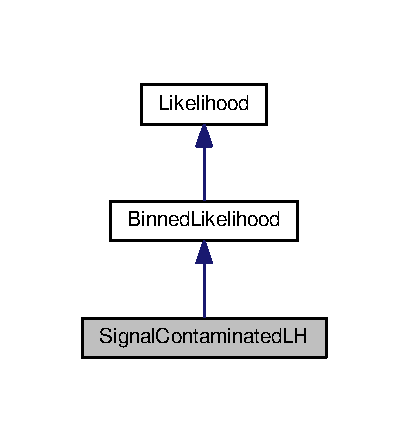
\includegraphics[width=196pt]{classSignalContaminatedLH__coll__graph}
\end{center}
\end{figure}
\subsection*{Public Types}
\begin{DoxyCompactItemize}
\item 
enum \hyperlink{classSignalContaminatedLH_a9d4a8fe949ffa894ce3dc79a79257c39}{Model} \{ \hyperlink{classSignalContaminatedLH_a9d4a8fe949ffa894ce3dc79a79257c39a938925ccf594ff61ad6259e1cbad39ad}{None}, 
\hyperlink{classSignalContaminatedLH_a9d4a8fe949ffa894ce3dc79a79257c39acb9f8cfccc9a6e01055b7abbe18aca40}{Poisson}, 
\hyperlink{classSignalContaminatedLH_a9d4a8fe949ffa894ce3dc79a79257c39aaa0cea64560f39edb1f5cdc6fa2c8b27}{Binomial}
 \}
\end{DoxyCompactItemize}
\subsection*{Public Member Functions}
\begin{DoxyCompactItemize}
\item 
\hyperlink{classSignalContaminatedLH_adcc85279f2683e800839bf9b1d837a53}{Signal\-Contaminated\-L\-H} (const \hyperlink{classDistribution}{Distribution} \&signal, const \hyperlink{classDistribution}{Distribution} \&background, const \hyperlink{classDistribution}{Distribution} \&signal\-Scrambled, const \hyperlink{classDistribution}{Distribution} \&signal\-Sample, const \hyperlink{classDistribution}{Distribution} \&background\-Sample, const \hyperlink{classDistribution}{Distribution} \&signal\-Scrambled\-Sample, double N, double sig\-\_\-prob=1.\-0, double bg\-\_\-prob=1.\-0, \hyperlink{classSignalContaminatedLH_a9d4a8fe949ffa894ce3dc79a79257c39}{Signal\-Contaminated\-L\-H\-::\-Model} model=\hyperlink{classSignalContaminatedLH_a9d4a8fe949ffa894ce3dc79a79257c39a938925ccf594ff61ad6259e1cbad39ad}{Signal\-Contaminated\-L\-H\-::\-None}, double sig\-\_\-sample\-\_\-prob=1.\-0, double bg\-\_\-sample\-\_\-prob=1.\-0, int seed=1)
\item 
double \hyperlink{classSignalContaminatedLH_a30c729fa905cc0d812827f23c71b55cc}{Evaluate\-L\-L\-H} (double xi) const 
\item 
\hyperlink{classSignalContaminatedLH_a9d4a8fe949ffa894ce3dc79a79257c39}{Model} \hyperlink{classSignalContaminatedLH_a07dbde7a99bf6b3063a933f2a53f48a1}{Get\-Model} ()
\item 
const \hyperlink{classDistribution}{Distribution} \& \hyperlink{classSignalContaminatedLH_a4172a3ca2e8261150d5008886342529f}{Get\-Signal\-P\-D\-F} () const 
\item 
const \hyperlink{classDistribution}{Distribution} \& \hyperlink{classSignalContaminatedLH_a6c6990779ac1e9b26eb1468944109760}{Get\-Bg\-P\-D\-F} () const 
\item 
void \hyperlink{classSignalContaminatedLH_a04fcf69547f8b0c5bc3ee2cb89671c06}{Sample\-Events} (double xi)
\begin{DoxyCompactList}\small\item\em Creates internally a new sample with the specified parameter. \end{DoxyCompactList}\item 
uint64\-\_\-t \hyperlink{classSignalContaminatedLH_abc5929f588d9e1944010e303ce66abf7}{Get\-N\-Events} ()
\item 
double \hyperlink{classSignalContaminatedLH_a9e201ec323c7d849151bde4b0d0ac82a}{Xi2\-W} (double xi) const 
\item 
double \hyperlink{classSignalContaminatedLH_ad39354a351421539c3e7fd136398b7b5}{W2\-Xi} (double w) const 
\item 
double \hyperlink{classSignalContaminatedLH_a72c6b5f9c339214cbd8e3fe41c9bad5d}{W2\-Mu} (double w) const 
\item 
double \hyperlink{classSignalContaminatedLH_a7fa94978c4da27077a38818e3baf0e19}{Xi2\-Mu} (double xi) const 
\item 
double \hyperlink{classSignalContaminatedLH_a151bf309a577282e09dbb75566c1467e}{Mu2\-Xi} (double mu) const 
\item 
void \hyperlink{classSignalContaminatedLH_ad991e7649ed72c411830cb0c7788dff4}{Minimizer\-Conditions} (\hyperlink{classMinimizer}{Minimizer} \&min)
\item 
\hyperlink{Likelihood_8h_a97d92c5c141f28319e7e8198defc9084}{likelihood\-Callback} \hyperlink{classSignalContaminatedLH_a9c67422f6e79df2352bd158be9949feb}{Call\-Back\-Fcn} ()
\begin{DoxyCompactList}\small\item\em Return the callback function of the likelihood for the minimizer. \end{DoxyCompactList}\item 
\hyperlink{classSignalContaminatedLH}{Signal\-Contaminated\-L\-H} $\ast$ \hyperlink{classSignalContaminatedLH_ae7c8264a79340a12dd4a83d83f0b9d2f}{Clone} (int seed) const 
\item 
double \hyperlink{classSignalContaminatedLH_a579d86a266c6ecb44cff26e47d141a9e}{Max\-Xi\-Bound} ()
\end{DoxyCompactItemize}
\subsection*{Additional Inherited Members}


\subsection{Member Enumeration Documentation}
\hypertarget{classSignalContaminatedLH_a9d4a8fe949ffa894ce3dc79a79257c39}{\index{Signal\-Contaminated\-L\-H@{Signal\-Contaminated\-L\-H}!Model@{Model}}
\index{Model@{Model}!SignalContaminatedLH@{Signal\-Contaminated\-L\-H}}
\subsubsection[{Model}]{\setlength{\rightskip}{0pt plus 5cm}enum {\bf Signal\-Contaminated\-L\-H\-::\-Model}}}\label{classSignalContaminatedLH_a9d4a8fe949ffa894ce3dc79a79257c39}
\begin{Desc}
\item[Enumerator]\par
\begin{description}
\index{None@{None}!Signal\-Contaminated\-L\-H@{Signal\-Contaminated\-L\-H}}\index{Signal\-Contaminated\-L\-H@{Signal\-Contaminated\-L\-H}!None@{None}}\item[{\em 
\hypertarget{classSignalContaminatedLH_a9d4a8fe949ffa894ce3dc79a79257c39a938925ccf594ff61ad6259e1cbad39ad}{None}\label{classSignalContaminatedLH_a9d4a8fe949ffa894ce3dc79a79257c39a938925ccf594ff61ad6259e1cbad39ad}
}]\index{Poisson@{Poisson}!Signal\-Contaminated\-L\-H@{Signal\-Contaminated\-L\-H}}\index{Signal\-Contaminated\-L\-H@{Signal\-Contaminated\-L\-H}!Poisson@{Poisson}}\item[{\em 
\hypertarget{classSignalContaminatedLH_a9d4a8fe949ffa894ce3dc79a79257c39acb9f8cfccc9a6e01055b7abbe18aca40}{Poisson}\label{classSignalContaminatedLH_a9d4a8fe949ffa894ce3dc79a79257c39acb9f8cfccc9a6e01055b7abbe18aca40}
}]\index{Binomial@{Binomial}!Signal\-Contaminated\-L\-H@{Signal\-Contaminated\-L\-H}}\index{Signal\-Contaminated\-L\-H@{Signal\-Contaminated\-L\-H}!Binomial@{Binomial}}\item[{\em 
\hypertarget{classSignalContaminatedLH_a9d4a8fe949ffa894ce3dc79a79257c39aaa0cea64560f39edb1f5cdc6fa2c8b27}{Binomial}\label{classSignalContaminatedLH_a9d4a8fe949ffa894ce3dc79a79257c39aaa0cea64560f39edb1f5cdc6fa2c8b27}
}]\end{description}
\end{Desc}


\subsection{Constructor \& Destructor Documentation}
\hypertarget{classSignalContaminatedLH_adcc85279f2683e800839bf9b1d837a53}{\index{Signal\-Contaminated\-L\-H@{Signal\-Contaminated\-L\-H}!Signal\-Contaminated\-L\-H@{Signal\-Contaminated\-L\-H}}
\index{Signal\-Contaminated\-L\-H@{Signal\-Contaminated\-L\-H}!SignalContaminatedLH@{Signal\-Contaminated\-L\-H}}
\subsubsection[{Signal\-Contaminated\-L\-H}]{\setlength{\rightskip}{0pt plus 5cm}Signal\-Contaminated\-L\-H\-::\-Signal\-Contaminated\-L\-H (
\begin{DoxyParamCaption}
\item[{const {\bf Distribution} \&}]{signal, }
\item[{const {\bf Distribution} \&}]{background, }
\item[{const {\bf Distribution} \&}]{signal\-Scrambled, }
\item[{const {\bf Distribution} \&}]{signal\-Sample, }
\item[{const {\bf Distribution} \&}]{background\-Sample, }
\item[{const {\bf Distribution} \&}]{signal\-Scrambled\-Sample, }
\item[{double}]{N, }
\item[{double}]{sig\-\_\-prob = {\ttfamily 1.0}, }
\item[{double}]{bg\-\_\-prob = {\ttfamily 1.0}, }
\item[{{\bf Signal\-Contaminated\-L\-H\-::\-Model}}]{model = {\ttfamily {\bf Signal\-Contaminated\-L\-H\-::\-None}}, }
\item[{double}]{sig\-\_\-sample\-\_\-prob = {\ttfamily 1.0}, }
\item[{double}]{bg\-\_\-sample\-\_\-prob = {\ttfamily 1.0}, }
\item[{int}]{seed = {\ttfamily 1}}
\end{DoxyParamCaption}
)}}\label{classSignalContaminatedLH_adcc85279f2683e800839bf9b1d837a53}


\subsection{Member Function Documentation}
\hypertarget{classSignalContaminatedLH_a9c67422f6e79df2352bd158be9949feb}{\index{Signal\-Contaminated\-L\-H@{Signal\-Contaminated\-L\-H}!Call\-Back\-Fcn@{Call\-Back\-Fcn}}
\index{Call\-Back\-Fcn@{Call\-Back\-Fcn}!SignalContaminatedLH@{Signal\-Contaminated\-L\-H}}
\subsubsection[{Call\-Back\-Fcn}]{\setlength{\rightskip}{0pt plus 5cm}{\bf likelihood\-Callback} Signal\-Contaminated\-L\-H\-::\-Call\-Back\-Fcn (
\begin{DoxyParamCaption}
{}
\end{DoxyParamCaption}
)\hspace{0.3cm}{\ttfamily [inline]}, {\ttfamily [virtual]}}}\label{classSignalContaminatedLH_a9c67422f6e79df2352bd158be9949feb}


Return the callback function of the likelihood for the minimizer. 



Implements \hyperlink{classBinnedLikelihood_aed7e05d58a36f515afc8e34fe8550b31}{Binned\-Likelihood}.

\hypertarget{classSignalContaminatedLH_ae7c8264a79340a12dd4a83d83f0b9d2f}{\index{Signal\-Contaminated\-L\-H@{Signal\-Contaminated\-L\-H}!Clone@{Clone}}
\index{Clone@{Clone}!SignalContaminatedLH@{Signal\-Contaminated\-L\-H}}
\subsubsection[{Clone}]{\setlength{\rightskip}{0pt plus 5cm}{\bf Signal\-Contaminated\-L\-H}$\ast$ Signal\-Contaminated\-L\-H\-::\-Clone (
\begin{DoxyParamCaption}
\item[{int}]{seed}
\end{DoxyParamCaption}
) const\hspace{0.3cm}{\ttfamily [inline]}, {\ttfamily [virtual]}}}\label{classSignalContaminatedLH_ae7c8264a79340a12dd4a83d83f0b9d2f}
Should create a copy of the original \hyperlink{classLikelihood}{Likelihood} which is thread safe. 

Implements \hyperlink{classLikelihood_a938b362a171c46f447cb364effc83bcf}{Likelihood}.

\hypertarget{classSignalContaminatedLH_a30c729fa905cc0d812827f23c71b55cc}{\index{Signal\-Contaminated\-L\-H@{Signal\-Contaminated\-L\-H}!Evaluate\-L\-L\-H@{Evaluate\-L\-L\-H}}
\index{Evaluate\-L\-L\-H@{Evaluate\-L\-L\-H}!SignalContaminatedLH@{Signal\-Contaminated\-L\-H}}
\subsubsection[{Evaluate\-L\-L\-H}]{\setlength{\rightskip}{0pt plus 5cm}double Signal\-Contaminated\-L\-H\-::\-Evaluate\-L\-L\-H (
\begin{DoxyParamCaption}
\item[{double}]{xi}
\end{DoxyParamCaption}
) const\hspace{0.3cm}{\ttfamily [virtual]}}}\label{classSignalContaminatedLH_a30c729fa905cc0d812827f23c71b55cc}
Evaluates the log likelihood sum 
\begin{DoxyParams}{Parameters}
{\em xi} & the signal fraction for which the likelihood should be evaulated. \\
\hline
\end{DoxyParams}


Implements \hyperlink{classBinnedLikelihood_a2084a64cd8b5d6bf8055538a0f633785}{Binned\-Likelihood}.

\hypertarget{classSignalContaminatedLH_a6c6990779ac1e9b26eb1468944109760}{\index{Signal\-Contaminated\-L\-H@{Signal\-Contaminated\-L\-H}!Get\-Bg\-P\-D\-F@{Get\-Bg\-P\-D\-F}}
\index{Get\-Bg\-P\-D\-F@{Get\-Bg\-P\-D\-F}!SignalContaminatedLH@{Signal\-Contaminated\-L\-H}}
\subsubsection[{Get\-Bg\-P\-D\-F}]{\setlength{\rightskip}{0pt plus 5cm}const {\bf Distribution}\& Signal\-Contaminated\-L\-H\-::\-Get\-Bg\-P\-D\-F (
\begin{DoxyParamCaption}
{}
\end{DoxyParamCaption}
) const\hspace{0.3cm}{\ttfamily [inline]}}}\label{classSignalContaminatedLH_a6c6990779ac1e9b26eb1468944109760}
\hypertarget{classSignalContaminatedLH_a07dbde7a99bf6b3063a933f2a53f48a1}{\index{Signal\-Contaminated\-L\-H@{Signal\-Contaminated\-L\-H}!Get\-Model@{Get\-Model}}
\index{Get\-Model@{Get\-Model}!SignalContaminatedLH@{Signal\-Contaminated\-L\-H}}
\subsubsection[{Get\-Model}]{\setlength{\rightskip}{0pt plus 5cm}{\bf Model} Signal\-Contaminated\-L\-H\-::\-Get\-Model (
\begin{DoxyParamCaption}
{}
\end{DoxyParamCaption}
)\hspace{0.3cm}{\ttfamily [inline]}}}\label{classSignalContaminatedLH_a07dbde7a99bf6b3063a933f2a53f48a1}
\hypertarget{classSignalContaminatedLH_abc5929f588d9e1944010e303ce66abf7}{\index{Signal\-Contaminated\-L\-H@{Signal\-Contaminated\-L\-H}!Get\-N\-Events@{Get\-N\-Events}}
\index{Get\-N\-Events@{Get\-N\-Events}!SignalContaminatedLH@{Signal\-Contaminated\-L\-H}}
\subsubsection[{Get\-N\-Events}]{\setlength{\rightskip}{0pt plus 5cm}uint64\-\_\-t Signal\-Contaminated\-L\-H\-::\-Get\-N\-Events (
\begin{DoxyParamCaption}
{}
\end{DoxyParamCaption}
)\hspace{0.3cm}{\ttfamily [inline]}}}\label{classSignalContaminatedLH_abc5929f588d9e1944010e303ce66abf7}
\hypertarget{classSignalContaminatedLH_a4172a3ca2e8261150d5008886342529f}{\index{Signal\-Contaminated\-L\-H@{Signal\-Contaminated\-L\-H}!Get\-Signal\-P\-D\-F@{Get\-Signal\-P\-D\-F}}
\index{Get\-Signal\-P\-D\-F@{Get\-Signal\-P\-D\-F}!SignalContaminatedLH@{Signal\-Contaminated\-L\-H}}
\subsubsection[{Get\-Signal\-P\-D\-F}]{\setlength{\rightskip}{0pt plus 5cm}const {\bf Distribution}\& Signal\-Contaminated\-L\-H\-::\-Get\-Signal\-P\-D\-F (
\begin{DoxyParamCaption}
{}
\end{DoxyParamCaption}
) const\hspace{0.3cm}{\ttfamily [inline]}}}\label{classSignalContaminatedLH_a4172a3ca2e8261150d5008886342529f}
\hypertarget{classSignalContaminatedLH_a579d86a266c6ecb44cff26e47d141a9e}{\index{Signal\-Contaminated\-L\-H@{Signal\-Contaminated\-L\-H}!Max\-Xi\-Bound@{Max\-Xi\-Bound}}
\index{Max\-Xi\-Bound@{Max\-Xi\-Bound}!SignalContaminatedLH@{Signal\-Contaminated\-L\-H}}
\subsubsection[{Max\-Xi\-Bound}]{\setlength{\rightskip}{0pt plus 5cm}double Signal\-Contaminated\-L\-H\-::\-Max\-Xi\-Bound (
\begin{DoxyParamCaption}
{}
\end{DoxyParamCaption}
)\hspace{0.3cm}{\ttfamily [inline]}, {\ttfamily [virtual]}}}\label{classSignalContaminatedLH_a579d86a266c6ecb44cff26e47d141a9e}


Reimplemented from \hyperlink{classBinnedLikelihood_ab6144b4d092744dc9d5ee58a491bf77d}{Binned\-Likelihood}.

\hypertarget{classSignalContaminatedLH_ad991e7649ed72c411830cb0c7788dff4}{\index{Signal\-Contaminated\-L\-H@{Signal\-Contaminated\-L\-H}!Minimizer\-Conditions@{Minimizer\-Conditions}}
\index{Minimizer\-Conditions@{Minimizer\-Conditions}!SignalContaminatedLH@{Signal\-Contaminated\-L\-H}}
\subsubsection[{Minimizer\-Conditions}]{\setlength{\rightskip}{0pt plus 5cm}void Signal\-Contaminated\-L\-H\-::\-Minimizer\-Conditions (
\begin{DoxyParamCaption}
\item[{{\bf Minimizer} \&}]{min}
\end{DoxyParamCaption}
)\hspace{0.3cm}{\ttfamily [virtual]}}}\label{classSignalContaminatedLH_ad991e7649ed72c411830cb0c7788dff4}


Reimplemented from \hyperlink{classLikelihood_ae43d17adaa0b34b9da4948e262b8d898}{Likelihood}.

\hypertarget{classSignalContaminatedLH_a151bf309a577282e09dbb75566c1467e}{\index{Signal\-Contaminated\-L\-H@{Signal\-Contaminated\-L\-H}!Mu2\-Xi@{Mu2\-Xi}}
\index{Mu2\-Xi@{Mu2\-Xi}!SignalContaminatedLH@{Signal\-Contaminated\-L\-H}}
\subsubsection[{Mu2\-Xi}]{\setlength{\rightskip}{0pt plus 5cm}double Signal\-Contaminated\-L\-H\-::\-Mu2\-Xi (
\begin{DoxyParamCaption}
\item[{double}]{mu}
\end{DoxyParamCaption}
) const\hspace{0.3cm}{\ttfamily [inline]}}}\label{classSignalContaminatedLH_a151bf309a577282e09dbb75566c1467e}
\hypertarget{classSignalContaminatedLH_a04fcf69547f8b0c5bc3ee2cb89671c06}{\index{Signal\-Contaminated\-L\-H@{Signal\-Contaminated\-L\-H}!Sample\-Events@{Sample\-Events}}
\index{Sample\-Events@{Sample\-Events}!SignalContaminatedLH@{Signal\-Contaminated\-L\-H}}
\subsubsection[{Sample\-Events}]{\setlength{\rightskip}{0pt plus 5cm}void Signal\-Contaminated\-L\-H\-::\-Sample\-Events (
\begin{DoxyParamCaption}
\item[{double}]{xi}
\end{DoxyParamCaption}
)\hspace{0.3cm}{\ttfamily [virtual]}}}\label{classSignalContaminatedLH_a04fcf69547f8b0c5bc3ee2cb89671c06}


Creates internally a new sample with the specified parameter. 



Implements \hyperlink{classBinnedLikelihood_a0793b8109912c6e509470a14a58d2a2a}{Binned\-Likelihood}.

\hypertarget{classSignalContaminatedLH_a72c6b5f9c339214cbd8e3fe41c9bad5d}{\index{Signal\-Contaminated\-L\-H@{Signal\-Contaminated\-L\-H}!W2\-Mu@{W2\-Mu}}
\index{W2\-Mu@{W2\-Mu}!SignalContaminatedLH@{Signal\-Contaminated\-L\-H}}
\subsubsection[{W2\-Mu}]{\setlength{\rightskip}{0pt plus 5cm}double Signal\-Contaminated\-L\-H\-::\-W2\-Mu (
\begin{DoxyParamCaption}
\item[{double}]{w}
\end{DoxyParamCaption}
) const\hspace{0.3cm}{\ttfamily [inline]}}}\label{classSignalContaminatedLH_a72c6b5f9c339214cbd8e3fe41c9bad5d}
\hypertarget{classSignalContaminatedLH_ad39354a351421539c3e7fd136398b7b5}{\index{Signal\-Contaminated\-L\-H@{Signal\-Contaminated\-L\-H}!W2\-Xi@{W2\-Xi}}
\index{W2\-Xi@{W2\-Xi}!SignalContaminatedLH@{Signal\-Contaminated\-L\-H}}
\subsubsection[{W2\-Xi}]{\setlength{\rightskip}{0pt plus 5cm}double Signal\-Contaminated\-L\-H\-::\-W2\-Xi (
\begin{DoxyParamCaption}
\item[{double}]{w}
\end{DoxyParamCaption}
) const\hspace{0.3cm}{\ttfamily [inline]}}}\label{classSignalContaminatedLH_ad39354a351421539c3e7fd136398b7b5}
\hypertarget{classSignalContaminatedLH_a7fa94978c4da27077a38818e3baf0e19}{\index{Signal\-Contaminated\-L\-H@{Signal\-Contaminated\-L\-H}!Xi2\-Mu@{Xi2\-Mu}}
\index{Xi2\-Mu@{Xi2\-Mu}!SignalContaminatedLH@{Signal\-Contaminated\-L\-H}}
\subsubsection[{Xi2\-Mu}]{\setlength{\rightskip}{0pt plus 5cm}double Signal\-Contaminated\-L\-H\-::\-Xi2\-Mu (
\begin{DoxyParamCaption}
\item[{double}]{xi}
\end{DoxyParamCaption}
) const\hspace{0.3cm}{\ttfamily [inline]}}}\label{classSignalContaminatedLH_a7fa94978c4da27077a38818e3baf0e19}
\hypertarget{classSignalContaminatedLH_a9e201ec323c7d849151bde4b0d0ac82a}{\index{Signal\-Contaminated\-L\-H@{Signal\-Contaminated\-L\-H}!Xi2\-W@{Xi2\-W}}
\index{Xi2\-W@{Xi2\-W}!SignalContaminatedLH@{Signal\-Contaminated\-L\-H}}
\subsubsection[{Xi2\-W}]{\setlength{\rightskip}{0pt plus 5cm}double Signal\-Contaminated\-L\-H\-::\-Xi2\-W (
\begin{DoxyParamCaption}
\item[{double}]{xi}
\end{DoxyParamCaption}
) const\hspace{0.3cm}{\ttfamily [inline]}}}\label{classSignalContaminatedLH_a9e201ec323c7d849151bde4b0d0ac82a}


The documentation for this class was generated from the following files\-:\begin{DoxyCompactItemize}
\item 
/home/travis/build/sflis/\-M\-L\-Sandbox/public/\-M\-L\-Sandbox/\hyperlink{SignalContaminatedLH_8h}{Signal\-Contaminated\-L\-H.\-h}\item 
/home/travis/build/sflis/\-M\-L\-Sandbox/private/\-M\-L\-Sandbox/\hyperlink{SignalContaminatedLH_8cxx}{Signal\-Contaminated\-L\-H.\-cxx}\end{DoxyCompactItemize}

\chapter{File Documentation}
\hypertarget{CombinedLikelihood_8cxx}{\section{/home/travis/build/sflis/\-M\-L\-Sandbox/private/\-M\-L\-Sandbox/\-Combined\-Likelihood.cxx File Reference}
\label{CombinedLikelihood_8cxx}\index{/home/travis/build/sflis/\-M\-L\-Sandbox/private/\-M\-L\-Sandbox/\-Combined\-Likelihood.\-cxx@{/home/travis/build/sflis/\-M\-L\-Sandbox/private/\-M\-L\-Sandbox/\-Combined\-Likelihood.\-cxx}}
}
{\ttfamily \#include \char`\"{}M\-L\-Sandbox/\-Combined\-Likelihood.\-h\char`\"{}}\\*
{\ttfamily \#include $<$math.\-h$>$}\\*
{\ttfamily \#include $<$iostream$>$}\\*
{\ttfamily \#include $<$cfloat$>$}\\*
{\ttfamily \#include $<$numeric$>$}\\*
{\ttfamily \#include $<$stdexcept$>$}\\*
Include dependency graph for Combined\-Likelihood.\-cxx\-:
\nopagebreak
\begin{figure}[H]
\begin{center}
\leavevmode
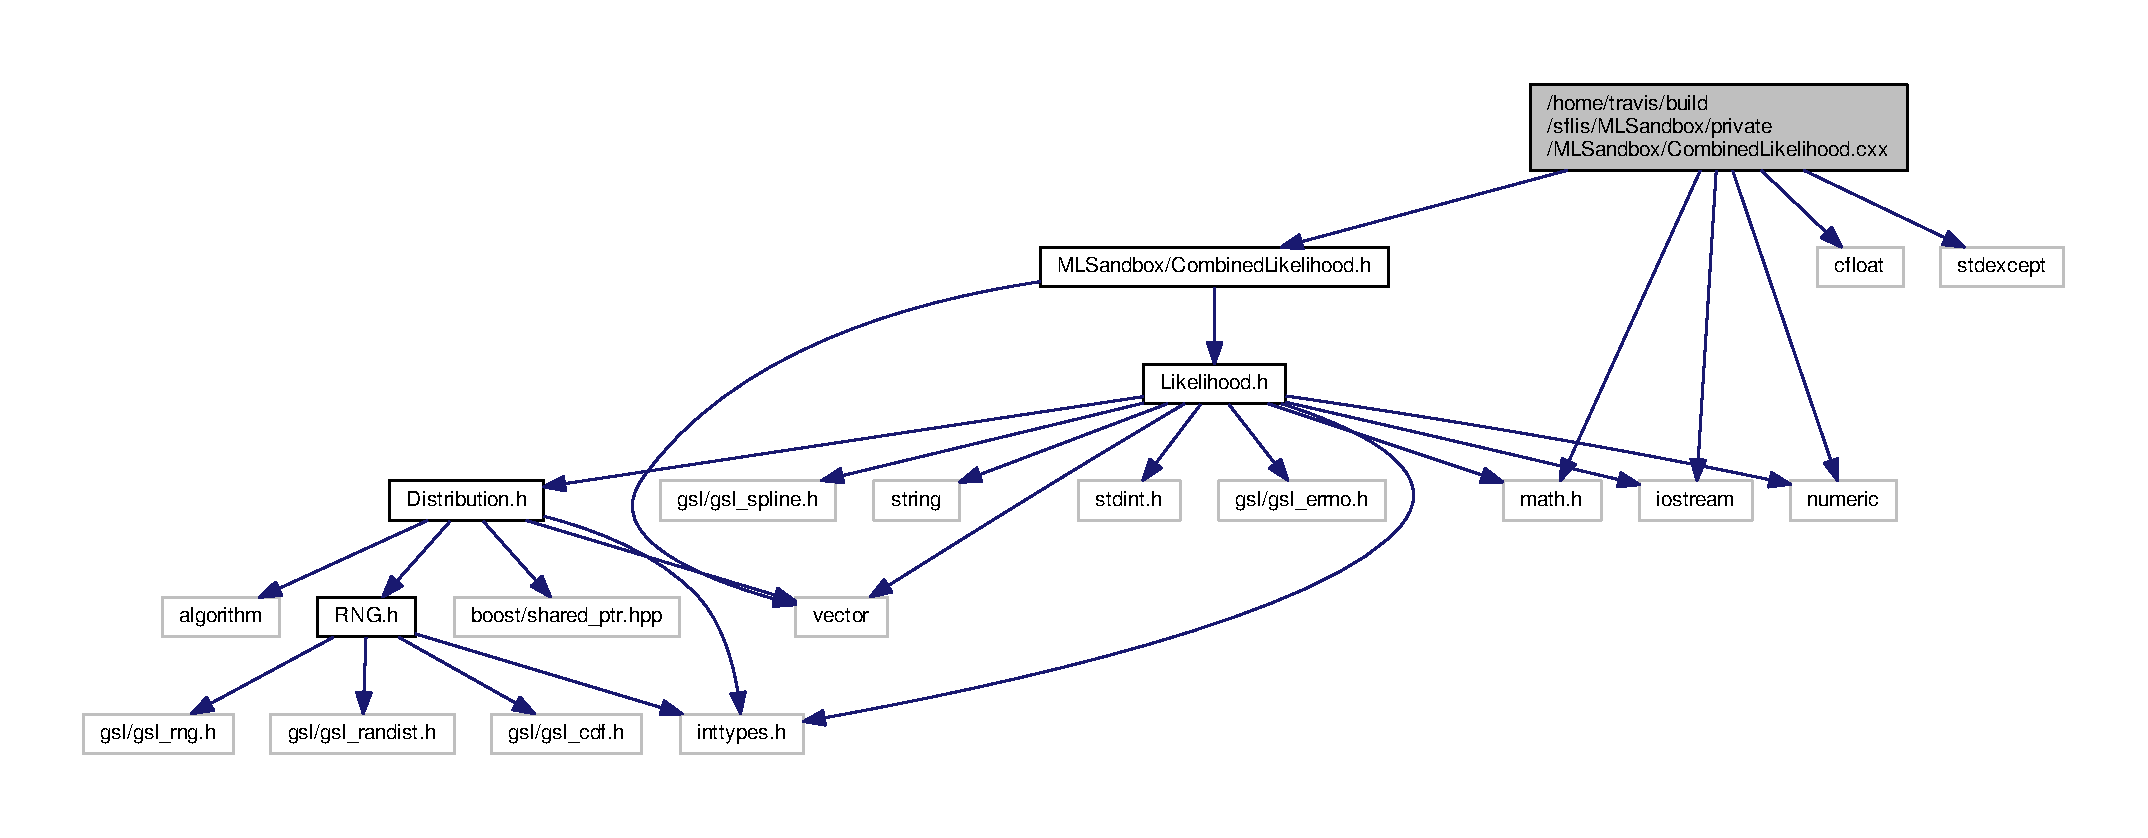
\includegraphics[width=350pt]{CombinedLikelihood_8cxx__incl}
\end{center}
\end{figure}

\hypertarget{MLSandbox_2Distribution_8cxx}{\section{/home/travis/build/sflis/\-M\-L\-Sandbox/private/\-M\-L\-Sandbox/\-Distribution.cxx File Reference}
\label{MLSandbox_2Distribution_8cxx}\index{/home/travis/build/sflis/\-M\-L\-Sandbox/private/\-M\-L\-Sandbox/\-Distribution.\-cxx@{/home/travis/build/sflis/\-M\-L\-Sandbox/private/\-M\-L\-Sandbox/\-Distribution.\-cxx}}
}
{\ttfamily \#include \char`\"{}M\-L\-Sandbox/\-Distribution.\-h\char`\"{}}\\*
{\ttfamily \#include $<$gsl/gsl\-\_\-rng.\-h$>$}\\*
{\ttfamily \#include $<$gsl/gsl\-\_\-randist.\-h$>$}\\*
{\ttfamily \#include $<$gsl/gsl\-\_\-cdf.\-h$>$}\\*
{\ttfamily \#include $<$math.\-h$>$}\\*
{\ttfamily \#include $<$iostream$>$}\\*
{\ttfamily \#include $<$vector$>$}\\*
{\ttfamily \#include $<$cfloat$>$}\\*
{\ttfamily \#include $<$algorithm$>$}\\*
{\ttfamily \#include $<$numeric$>$}\\*
{\ttfamily \#include $<$limits$>$}\\*
{\ttfamily \#include $<$stdexcept$>$}\\*
Include dependency graph for Distribution.\-cxx\-:
\nopagebreak
\begin{figure}[H]
\begin{center}
\leavevmode
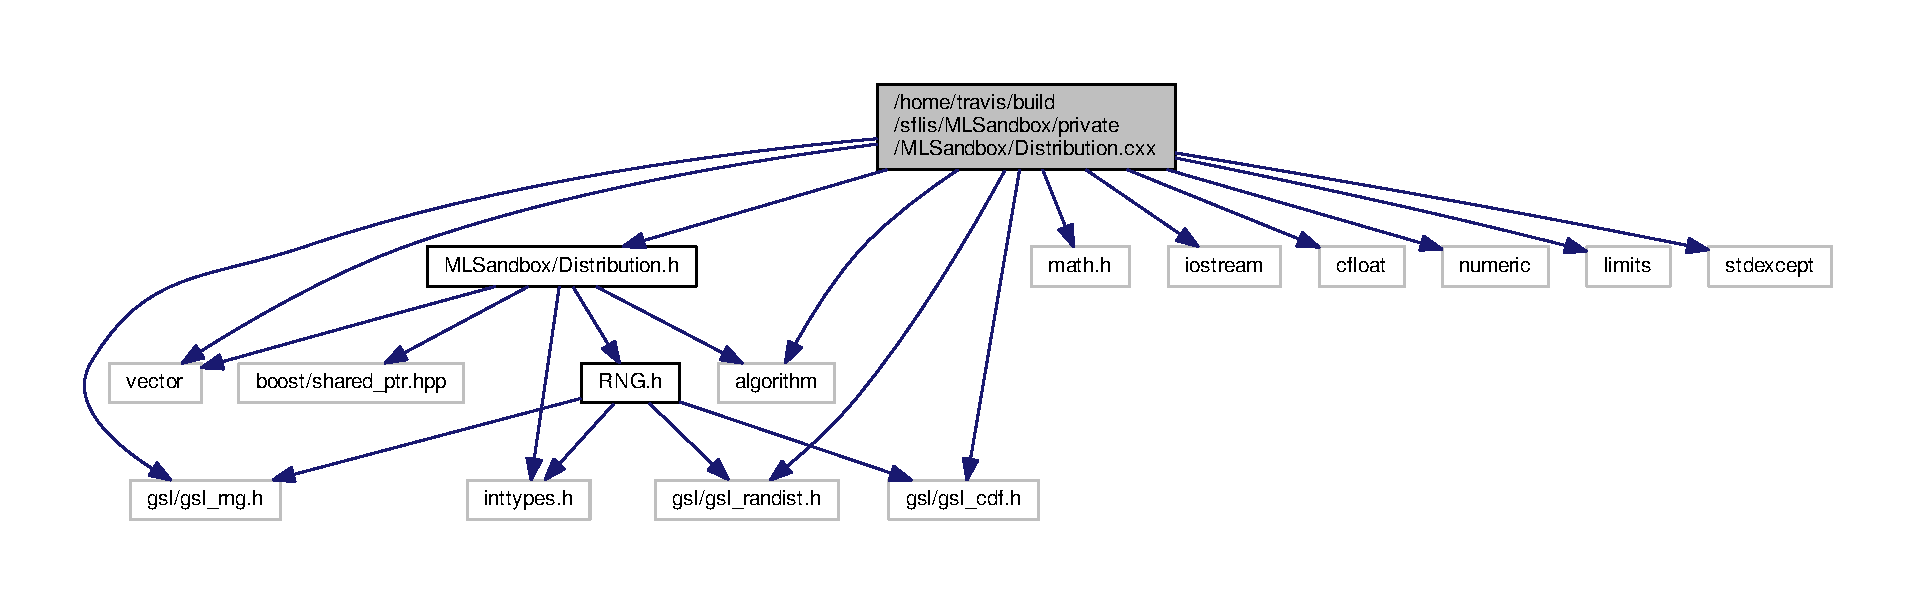
\includegraphics[width=350pt]{MLSandbox_2Distribution_8cxx__incl}
\end{center}
\end{figure}

\hypertarget{pybindings_2Distribution_8cxx}{\section{/home/travis/build/sflis/\-M\-L\-Sandbox/private/pybindings/\-Distribution.cxx File Reference}
\label{pybindings_2Distribution_8cxx}\index{/home/travis/build/sflis/\-M\-L\-Sandbox/private/pybindings/\-Distribution.\-cxx@{/home/travis/build/sflis/\-M\-L\-Sandbox/private/pybindings/\-Distribution.\-cxx}}
}
{\ttfamily \#include \char`\"{}M\-L\-Sandbox/\-Distribution.\-h\char`\"{}}\\*
{\ttfamily \#include $<$boost/numpy.\-hpp$>$}\\*
{\ttfamily \#include $<$iostream$>$}\\*
Include dependency graph for Distribution.\-cxx\-:
\nopagebreak
\begin{figure}[H]
\begin{center}
\leavevmode
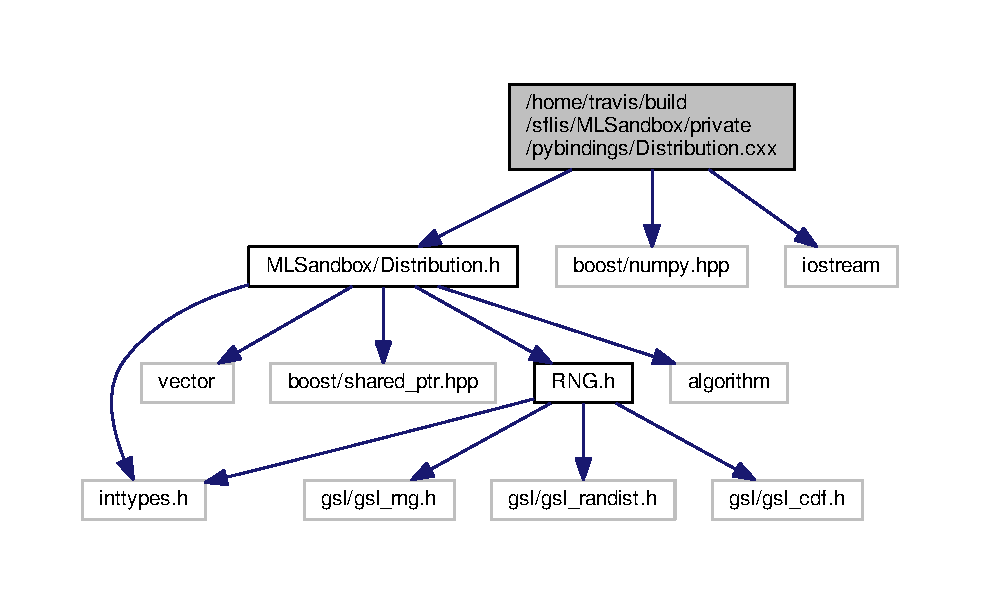
\includegraphics[width=350pt]{pybindings_2Distribution_8cxx__incl}
\end{center}
\end{figure}
\subsection*{Namespaces}
\begin{DoxyCompactItemize}
\item 
\hyperlink{namespacemlsandbox}{mlsandbox}
\item 
\hyperlink{namespacemlsandbox_1_1python}{mlsandbox\-::python}
\end{DoxyCompactItemize}
\subsection*{Functions}
\begin{DoxyCompactItemize}
\item 
boost\-::shared\-\_\-ptr$<$ \hyperlink{classDistribution}{Distribution} $>$ \hyperlink{namespacemlsandbox_1_1python_aa2d95d46d684b8e8a9e6041e6753904e}{mlsandbox\-::python\-::distribtion\-\_\-constructor} (bp\-::object distribution, double r\-Min, double r\-Max, uint r\-Seed)
\item 
bn\-::ndarray \hyperlink{namespacemlsandbox_1_1python_a00273dd6c5be90398654d4e7c707add4}{mlsandbox\-::python\-::sample} (\hyperlink{classDistribution}{Distribution} \&self, int N)
\item 
bn\-::ndarray \hyperlink{namespacemlsandbox_1_1python_a2a2c84be9021d9445d30be3d85447f9b}{mlsandbox\-::python\-::sample\-I} (\hyperlink{classDistribution}{Distribution} \&self, int N)
\item 
void \hyperlink{pybindings_2Distribution_8cxx_a6d75000cd59b9658b0b42b61a3913984}{register\-\_\-\-Distribution} ()
\end{DoxyCompactItemize}


\subsection{Function Documentation}
\hypertarget{pybindings_2Distribution_8cxx_a6d75000cd59b9658b0b42b61a3913984}{\index{pybindings/\-Distribution.\-cxx@{pybindings/\-Distribution.\-cxx}!register\-\_\-\-Distribution@{register\-\_\-\-Distribution}}
\index{register\-\_\-\-Distribution@{register\-\_\-\-Distribution}!pybindings/Distribution.cxx@{pybindings/\-Distribution.\-cxx}}
\subsubsection[{register\-\_\-\-Distribution}]{\setlength{\rightskip}{0pt plus 5cm}void register\-\_\-\-Distribution (
\begin{DoxyParamCaption}
{}
\end{DoxyParamCaption}
)}}\label{pybindings_2Distribution_8cxx_a6d75000cd59b9658b0b42b61a3913984}

\hypertarget{MLSandbox_2FCRanks_8cxx}{\section{/home/travis/build/sflis/\-M\-L\-Sandbox/private/\-M\-L\-Sandbox/\-F\-C\-Ranks.cxx File Reference}
\label{MLSandbox_2FCRanks_8cxx}\index{/home/travis/build/sflis/\-M\-L\-Sandbox/private/\-M\-L\-Sandbox/\-F\-C\-Ranks.\-cxx@{/home/travis/build/sflis/\-M\-L\-Sandbox/private/\-M\-L\-Sandbox/\-F\-C\-Ranks.\-cxx}}
}
{\ttfamily \#include \char`\"{}M\-L\-Sandbox/\-F\-C\-Ranks.\-h\char`\"{}}\\*
{\ttfamily \#include $<$fstream$>$}\\*
{\ttfamily \#include $<$iostream$>$}\\*
{\ttfamily \#include $<$boost/archive/binary\-\_\-oarchive.\-hpp$>$}\\*
{\ttfamily \#include $<$boost/archive/binary\-\_\-iarchive.\-hpp$>$}\\*
{\ttfamily \#include $<$boost/serialization/base\-\_\-object.\-hpp$>$}\\*
{\ttfamily \#include $<$boost/serialization/map.\-hpp$>$}\\*
Include dependency graph for F\-C\-Ranks.\-cxx\-:
\nopagebreak
\begin{figure}[H]
\begin{center}
\leavevmode
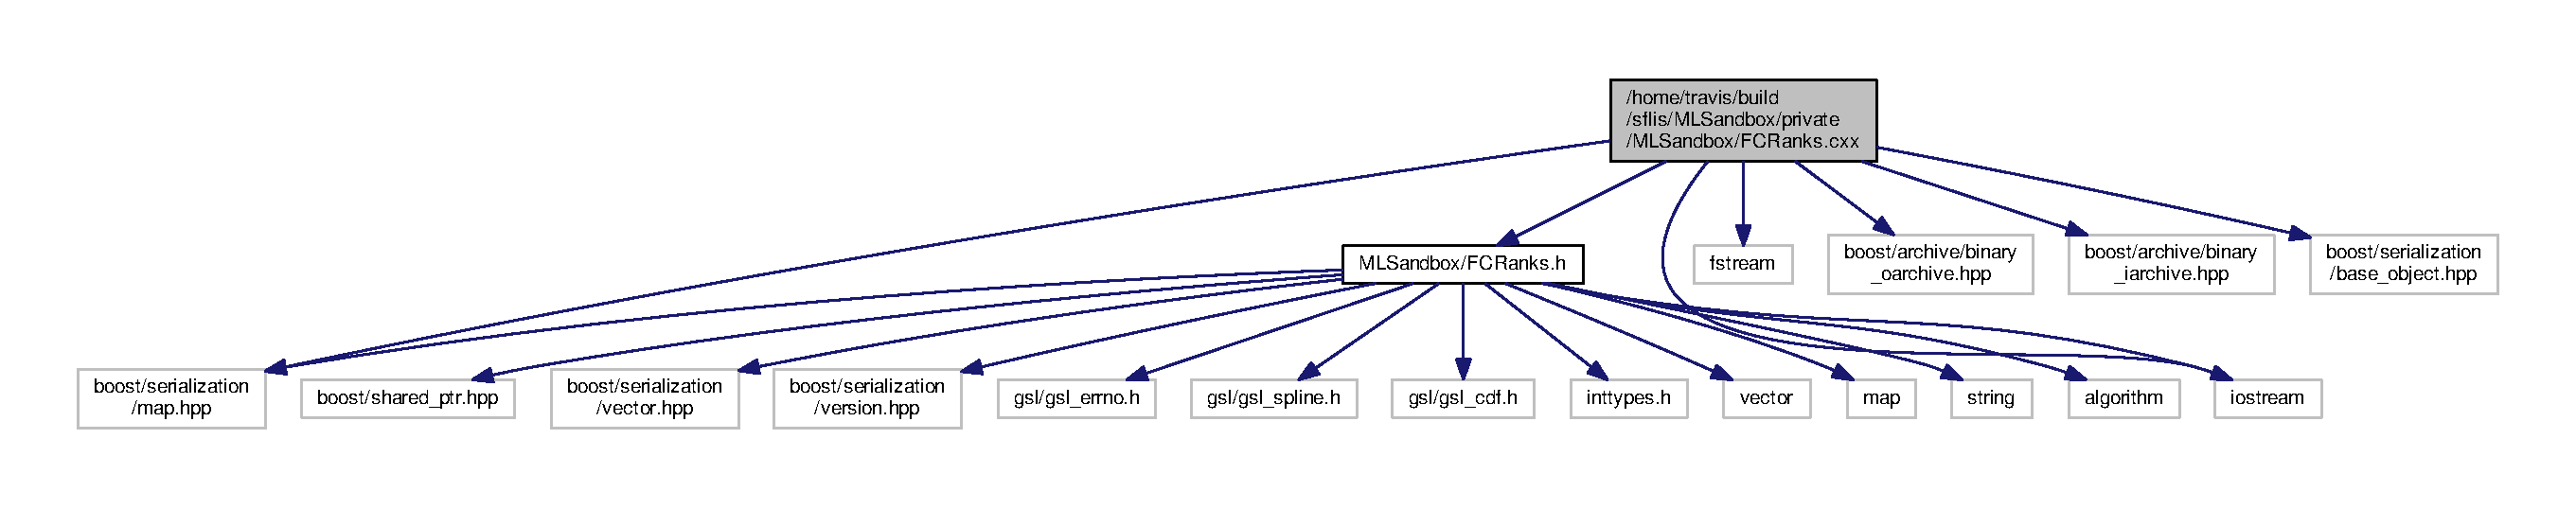
\includegraphics[width=350pt]{MLSandbox_2FCRanks_8cxx__incl}
\end{center}
\end{figure}

\hypertarget{pybindings_2FCRanks_8cxx}{\section{/home/travis/build/sflis/\-M\-L\-Sandbox/private/pybindings/\-F\-C\-Ranks.cxx File Reference}
\label{pybindings_2FCRanks_8cxx}\index{/home/travis/build/sflis/\-M\-L\-Sandbox/private/pybindings/\-F\-C\-Ranks.\-cxx@{/home/travis/build/sflis/\-M\-L\-Sandbox/private/pybindings/\-F\-C\-Ranks.\-cxx}}
}
{\ttfamily \#include \char`\"{}M\-L\-Sandbox/\-F\-C\-Ranks.\-h\char`\"{}}\\*
{\ttfamily \#include \char`\"{}bindingutils.\-h\char`\"{}}\\*
{\ttfamily \#include $<$boost/numpy.\-hpp$>$}\\*
{\ttfamily \#include $<$string$>$}\\*
{\ttfamily \#include $<$iostream$>$}\\*
Include dependency graph for F\-C\-Ranks.\-cxx\-:
\nopagebreak
\begin{figure}[H]
\begin{center}
\leavevmode
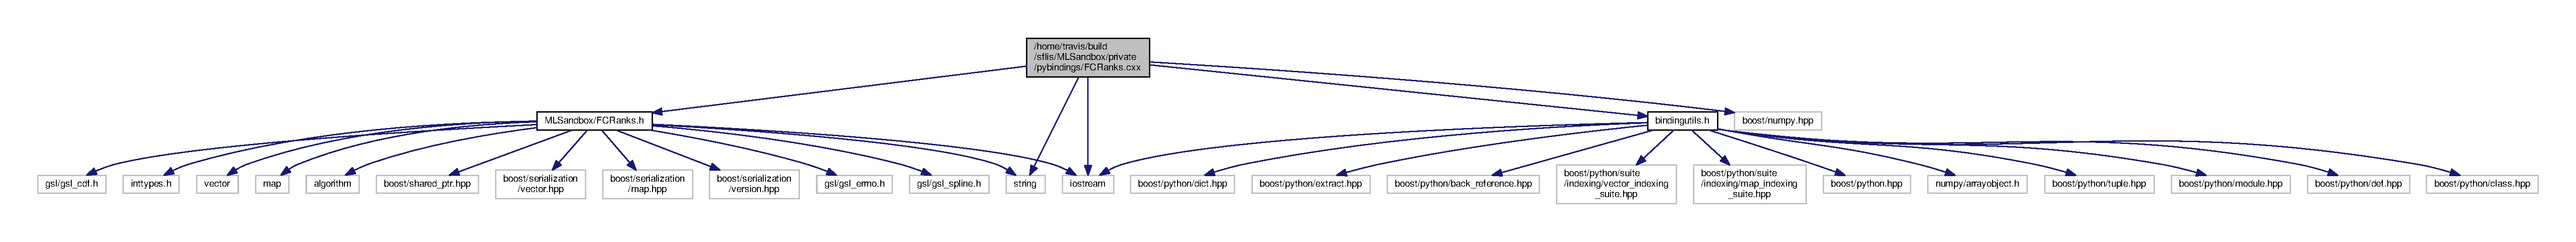
\includegraphics[width=350pt]{pybindings_2FCRanks_8cxx__incl}
\end{center}
\end{figure}
\subsection*{Namespaces}
\begin{DoxyCompactItemize}
\item 
\hyperlink{namespacemlsandbox}{mlsandbox}
\item 
\hyperlink{namespacemlsandbox_1_1python}{mlsandbox\-::python}
\end{DoxyCompactItemize}
\subsection*{Macros}
\begin{DoxyCompactItemize}
\item 
\#define \hyperlink{pybindings_2FCRanks_8cxx_ab6e6ee86736f9ebb56e74ae21bf3ff8a}{N\-P\-Y\-\_\-\-N\-O\-\_\-\-D\-E\-P\-R\-E\-C\-A\-T\-E\-D\-\_\-\-A\-P\-I}~N\-P\-Y\-\_\-1\-\_\-7\-\_\-\-A\-P\-I\-\_\-\-V\-E\-R\-S\-I\-O\-N
\end{DoxyCompactItemize}
\subsection*{Functions}
\begin{DoxyCompactItemize}
\item 
void \hyperlink{pybindings_2FCRanks_8cxx_aca5eee2e3eeaeaface3ed8cd1886d241}{register\-\_\-\-F\-C\-Ranks} ()
\end{DoxyCompactItemize}


\subsection{Macro Definition Documentation}
\hypertarget{pybindings_2FCRanks_8cxx_ab6e6ee86736f9ebb56e74ae21bf3ff8a}{\index{pybindings/\-F\-C\-Ranks.\-cxx@{pybindings/\-F\-C\-Ranks.\-cxx}!N\-P\-Y\-\_\-\-N\-O\-\_\-\-D\-E\-P\-R\-E\-C\-A\-T\-E\-D\-\_\-\-A\-P\-I@{N\-P\-Y\-\_\-\-N\-O\-\_\-\-D\-E\-P\-R\-E\-C\-A\-T\-E\-D\-\_\-\-A\-P\-I}}
\index{N\-P\-Y\-\_\-\-N\-O\-\_\-\-D\-E\-P\-R\-E\-C\-A\-T\-E\-D\-\_\-\-A\-P\-I@{N\-P\-Y\-\_\-\-N\-O\-\_\-\-D\-E\-P\-R\-E\-C\-A\-T\-E\-D\-\_\-\-A\-P\-I}!pybindings/FCRanks.cxx@{pybindings/\-F\-C\-Ranks.\-cxx}}
\subsubsection[{N\-P\-Y\-\_\-\-N\-O\-\_\-\-D\-E\-P\-R\-E\-C\-A\-T\-E\-D\-\_\-\-A\-P\-I}]{\setlength{\rightskip}{0pt plus 5cm}\#define N\-P\-Y\-\_\-\-N\-O\-\_\-\-D\-E\-P\-R\-E\-C\-A\-T\-E\-D\-\_\-\-A\-P\-I~N\-P\-Y\-\_\-1\-\_\-7\-\_\-\-A\-P\-I\-\_\-\-V\-E\-R\-S\-I\-O\-N}}\label{pybindings_2FCRanks_8cxx_ab6e6ee86736f9ebb56e74ae21bf3ff8a}


\subsection{Function Documentation}
\hypertarget{pybindings_2FCRanks_8cxx_aca5eee2e3eeaeaface3ed8cd1886d241}{\index{pybindings/\-F\-C\-Ranks.\-cxx@{pybindings/\-F\-C\-Ranks.\-cxx}!register\-\_\-\-F\-C\-Ranks@{register\-\_\-\-F\-C\-Ranks}}
\index{register\-\_\-\-F\-C\-Ranks@{register\-\_\-\-F\-C\-Ranks}!pybindings/FCRanks.cxx@{pybindings/\-F\-C\-Ranks.\-cxx}}
\subsubsection[{register\-\_\-\-F\-C\-Ranks}]{\setlength{\rightskip}{0pt plus 5cm}void register\-\_\-\-F\-C\-Ranks (
\begin{DoxyParamCaption}
{}
\end{DoxyParamCaption}
)}}\label{pybindings_2FCRanks_8cxx_aca5eee2e3eeaeaface3ed8cd1886d241}

\hypertarget{MLSandbox_2FeldmanCousins_8cxx}{\section{/home/travis/build/sflis/\-M\-L\-Sandbox/private/\-M\-L\-Sandbox/\-Feldman\-Cousins.cxx File Reference}
\label{MLSandbox_2FeldmanCousins_8cxx}\index{/home/travis/build/sflis/\-M\-L\-Sandbox/private/\-M\-L\-Sandbox/\-Feldman\-Cousins.\-cxx@{/home/travis/build/sflis/\-M\-L\-Sandbox/private/\-M\-L\-Sandbox/\-Feldman\-Cousins.\-cxx}}
}
{\ttfamily \#include \char`\"{}M\-L\-Sandbox/\-Feldman\-Cousins.\-h\char`\"{}}\\*
{\ttfamily \#include $<$gsl/gsl\-\_\-roots.\-h$>$}\\*
{\ttfamily \#include $<$gsl/gsl\-\_\-min.\-h$>$}\\*
{\ttfamily \#include $<$gsl/gsl\-\_\-errno.\-h$>$}\\*
{\ttfamily \#include $<$exception$>$}\\*
{\ttfamily \#include $<$stdexcept$>$}\\*
{\ttfamily \#include $<$pthread.\-h$>$}\\*
{\ttfamily \#include $<$string$>$}\\*
{\ttfamily \#include $<$iostream$>$}\\*
{\ttfamily \#include $<$iomanip$>$}\\*
{\ttfamily \#include $<$algorithm$>$}\\*
{\ttfamily \#include $<$queue$>$}\\*
{\ttfamily \#include $<$boost/make\-\_\-shared.\-hpp$>$}\\*
Include dependency graph for Feldman\-Cousins.\-cxx\-:
\nopagebreak
\begin{figure}[H]
\begin{center}
\leavevmode
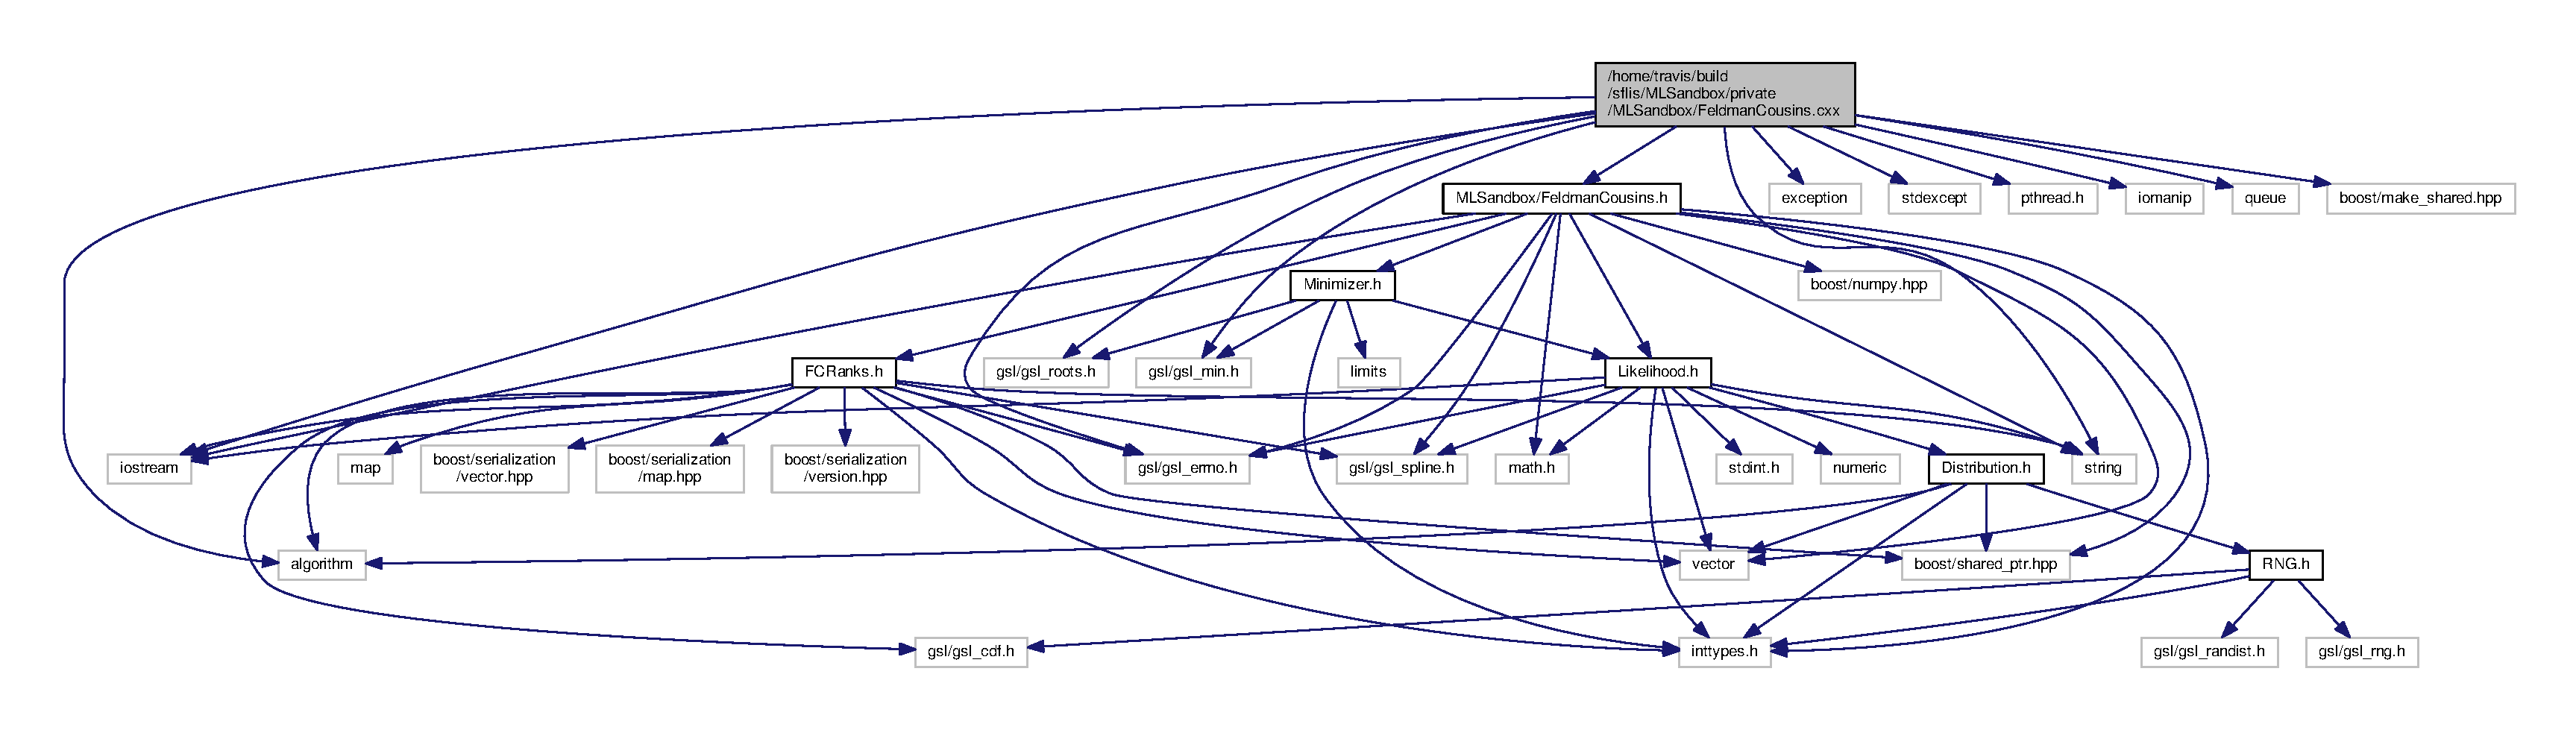
\includegraphics[width=350pt]{MLSandbox_2FeldmanCousins_8cxx__incl}
\end{center}
\end{figure}
\subsection*{Classes}
\begin{DoxyCompactItemize}
\item 
struct \hyperlink{structFCThreadData}{F\-C\-Thread\-Data}
\end{DoxyCompactItemize}
\subsection*{Functions}
\begin{DoxyCompactItemize}
\item 
void $\ast$ \hyperlink{MLSandbox_2FeldmanCousins_8cxx_a60929b09c20a8e046d404f63f819377a}{rank\-Computation\-Thread} (void $\ast$data)
\end{DoxyCompactItemize}
\subsection*{Variables}
\begin{DoxyCompactItemize}
\item 
pthread\-\_\-mutex\-\_\-t \hyperlink{MLSandbox_2FeldmanCousins_8cxx_aefc691d2e82892a7bcb11a3ffdb5b864}{mutex\-Fetch\-Hypothesis} = P\-T\-H\-R\-E\-A\-D\-\_\-\-M\-U\-T\-E\-X\-\_\-\-I\-N\-I\-T\-I\-A\-L\-I\-Z\-E\-R
\item 
pthread\-\_\-mutex\-\_\-t \hyperlink{MLSandbox_2FeldmanCousins_8cxx_a93b752a4a6a8f14b3d7d1b9241411580}{mutex\-Write\-Ranks} = P\-T\-H\-R\-E\-A\-D\-\_\-\-M\-U\-T\-E\-X\-\_\-\-I\-N\-I\-T\-I\-A\-L\-I\-Z\-E\-R
\end{DoxyCompactItemize}


\subsection{Function Documentation}
\hypertarget{MLSandbox_2FeldmanCousins_8cxx_a60929b09c20a8e046d404f63f819377a}{\index{M\-L\-Sandbox/\-Feldman\-Cousins.\-cxx@{M\-L\-Sandbox/\-Feldman\-Cousins.\-cxx}!rank\-Computation\-Thread@{rank\-Computation\-Thread}}
\index{rank\-Computation\-Thread@{rank\-Computation\-Thread}!MLSandbox/FeldmanCousins.cxx@{M\-L\-Sandbox/\-Feldman\-Cousins.\-cxx}}
\subsubsection[{rank\-Computation\-Thread}]{\setlength{\rightskip}{0pt plus 5cm}void $\ast$ rank\-Computation\-Thread (
\begin{DoxyParamCaption}
\item[{void $\ast$}]{data}
\end{DoxyParamCaption}
)}}\label{MLSandbox_2FeldmanCousins_8cxx_a60929b09c20a8e046d404f63f819377a}


\subsection{Variable Documentation}
\hypertarget{MLSandbox_2FeldmanCousins_8cxx_aefc691d2e82892a7bcb11a3ffdb5b864}{\index{M\-L\-Sandbox/\-Feldman\-Cousins.\-cxx@{M\-L\-Sandbox/\-Feldman\-Cousins.\-cxx}!mutex\-Fetch\-Hypothesis@{mutex\-Fetch\-Hypothesis}}
\index{mutex\-Fetch\-Hypothesis@{mutex\-Fetch\-Hypothesis}!MLSandbox/FeldmanCousins.cxx@{M\-L\-Sandbox/\-Feldman\-Cousins.\-cxx}}
\subsubsection[{mutex\-Fetch\-Hypothesis}]{\setlength{\rightskip}{0pt plus 5cm}pthread\-\_\-mutex\-\_\-t mutex\-Fetch\-Hypothesis = P\-T\-H\-R\-E\-A\-D\-\_\-\-M\-U\-T\-E\-X\-\_\-\-I\-N\-I\-T\-I\-A\-L\-I\-Z\-E\-R}}\label{MLSandbox_2FeldmanCousins_8cxx_aefc691d2e82892a7bcb11a3ffdb5b864}
\hypertarget{MLSandbox_2FeldmanCousins_8cxx_a93b752a4a6a8f14b3d7d1b9241411580}{\index{M\-L\-Sandbox/\-Feldman\-Cousins.\-cxx@{M\-L\-Sandbox/\-Feldman\-Cousins.\-cxx}!mutex\-Write\-Ranks@{mutex\-Write\-Ranks}}
\index{mutex\-Write\-Ranks@{mutex\-Write\-Ranks}!MLSandbox/FeldmanCousins.cxx@{M\-L\-Sandbox/\-Feldman\-Cousins.\-cxx}}
\subsubsection[{mutex\-Write\-Ranks}]{\setlength{\rightskip}{0pt plus 5cm}pthread\-\_\-mutex\-\_\-t mutex\-Write\-Ranks = P\-T\-H\-R\-E\-A\-D\-\_\-\-M\-U\-T\-E\-X\-\_\-\-I\-N\-I\-T\-I\-A\-L\-I\-Z\-E\-R}}\label{MLSandbox_2FeldmanCousins_8cxx_a93b752a4a6a8f14b3d7d1b9241411580}

\hypertarget{pybindings_2FeldmanCousins_8cxx}{\section{/home/travis/build/sflis/\-M\-L\-Sandbox/private/pybindings/\-Feldman\-Cousins.cxx File Reference}
\label{pybindings_2FeldmanCousins_8cxx}\index{/home/travis/build/sflis/\-M\-L\-Sandbox/private/pybindings/\-Feldman\-Cousins.\-cxx@{/home/travis/build/sflis/\-M\-L\-Sandbox/private/pybindings/\-Feldman\-Cousins.\-cxx}}
}
{\ttfamily \#include \char`\"{}M\-L\-Sandbox/\-Feldman\-Cousins.\-h\char`\"{}}\\*
{\ttfamily \#include $<$boost/numpy.\-hpp$>$}\\*
{\ttfamily \#include $<$boost/python/tuple.\-hpp$>$}\\*
{\ttfamily \#include $<$iostream$>$}\\*
{\ttfamily \#include $<$vector$>$}\\*
Include dependency graph for Feldman\-Cousins.\-cxx\-:
\nopagebreak
\begin{figure}[H]
\begin{center}
\leavevmode
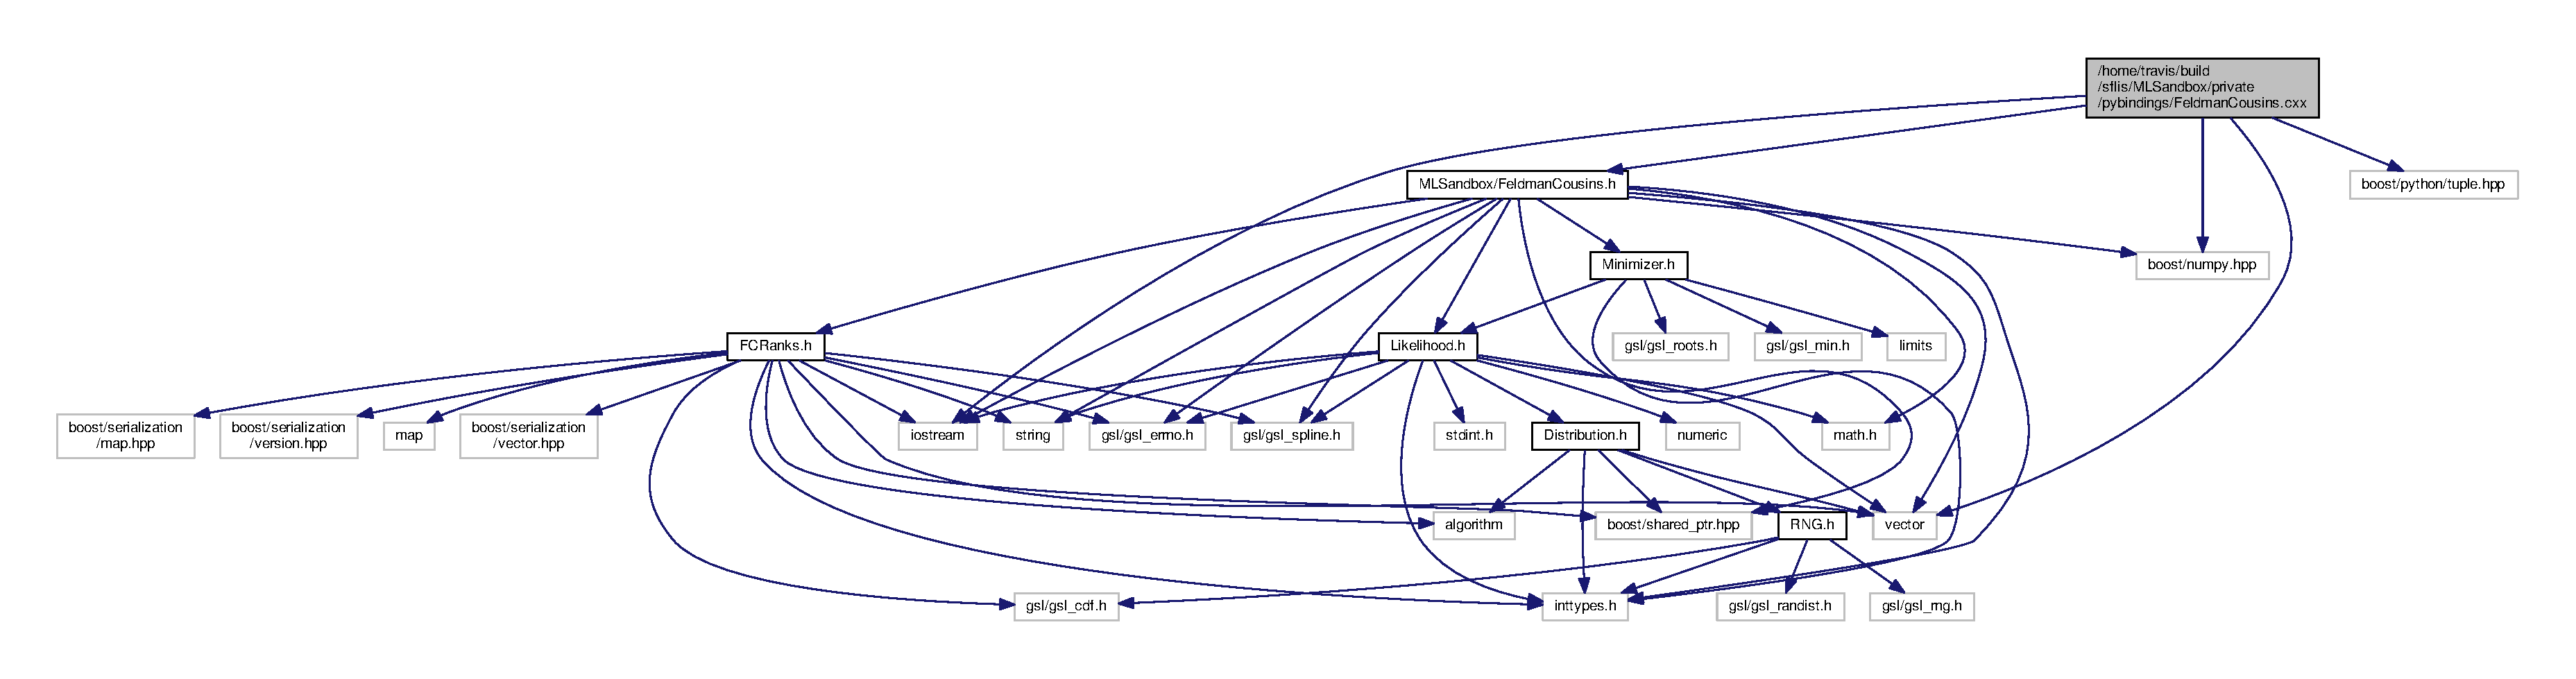
\includegraphics[width=350pt]{pybindings_2FeldmanCousins_8cxx__incl}
\end{center}
\end{figure}
\subsection*{Namespaces}
\begin{DoxyCompactItemize}
\item 
\hyperlink{namespacemlsandbox}{mlsandbox}
\item 
\hyperlink{namespacemlsandbox_1_1python}{mlsandbox\-::python}
\end{DoxyCompactItemize}
\subsection*{Functions}
\begin{DoxyCompactItemize}
\item 
void \hyperlink{pybindings_2FeldmanCousins_8cxx_a08cff9d3dff4125cda9df8308e41caff}{register\-\_\-\-Feldman\-Cousins} ()
\end{DoxyCompactItemize}


\subsection{Function Documentation}
\hypertarget{pybindings_2FeldmanCousins_8cxx_a08cff9d3dff4125cda9df8308e41caff}{\index{pybindings/\-Feldman\-Cousins.\-cxx@{pybindings/\-Feldman\-Cousins.\-cxx}!register\-\_\-\-Feldman\-Cousins@{register\-\_\-\-Feldman\-Cousins}}
\index{register\-\_\-\-Feldman\-Cousins@{register\-\_\-\-Feldman\-Cousins}!pybindings/FeldmanCousins.cxx@{pybindings/\-Feldman\-Cousins.\-cxx}}
\subsubsection[{register\-\_\-\-Feldman\-Cousins}]{\setlength{\rightskip}{0pt plus 5cm}void register\-\_\-\-Feldman\-Cousins (
\begin{DoxyParamCaption}
{}
\end{DoxyParamCaption}
)}}\label{pybindings_2FeldmanCousins_8cxx_a08cff9d3dff4125cda9df8308e41caff}

\hypertarget{MLSandbox_2Likelihood_8cxx}{\section{/home/travis/build/sflis/\-M\-L\-Sandbox/private/\-M\-L\-Sandbox/\-Likelihood.cxx File Reference}
\label{MLSandbox_2Likelihood_8cxx}\index{/home/travis/build/sflis/\-M\-L\-Sandbox/private/\-M\-L\-Sandbox/\-Likelihood.\-cxx@{/home/travis/build/sflis/\-M\-L\-Sandbox/private/\-M\-L\-Sandbox/\-Likelihood.\-cxx}}
}
{\ttfamily \#include \char`\"{}M\-L\-Sandbox/\-Likelihood.\-h\char`\"{}}\\*
{\ttfamily \#include $<$math.\-h$>$}\\*
{\ttfamily \#include $<$iostream$>$}\\*
{\ttfamily \#include $<$cfloat$>$}\\*
{\ttfamily \#include $<$numeric$>$}\\*
{\ttfamily \#include $<$stdexcept$>$}\\*
Include dependency graph for Likelihood.\-cxx\-:
\nopagebreak
\begin{figure}[H]
\begin{center}
\leavevmode
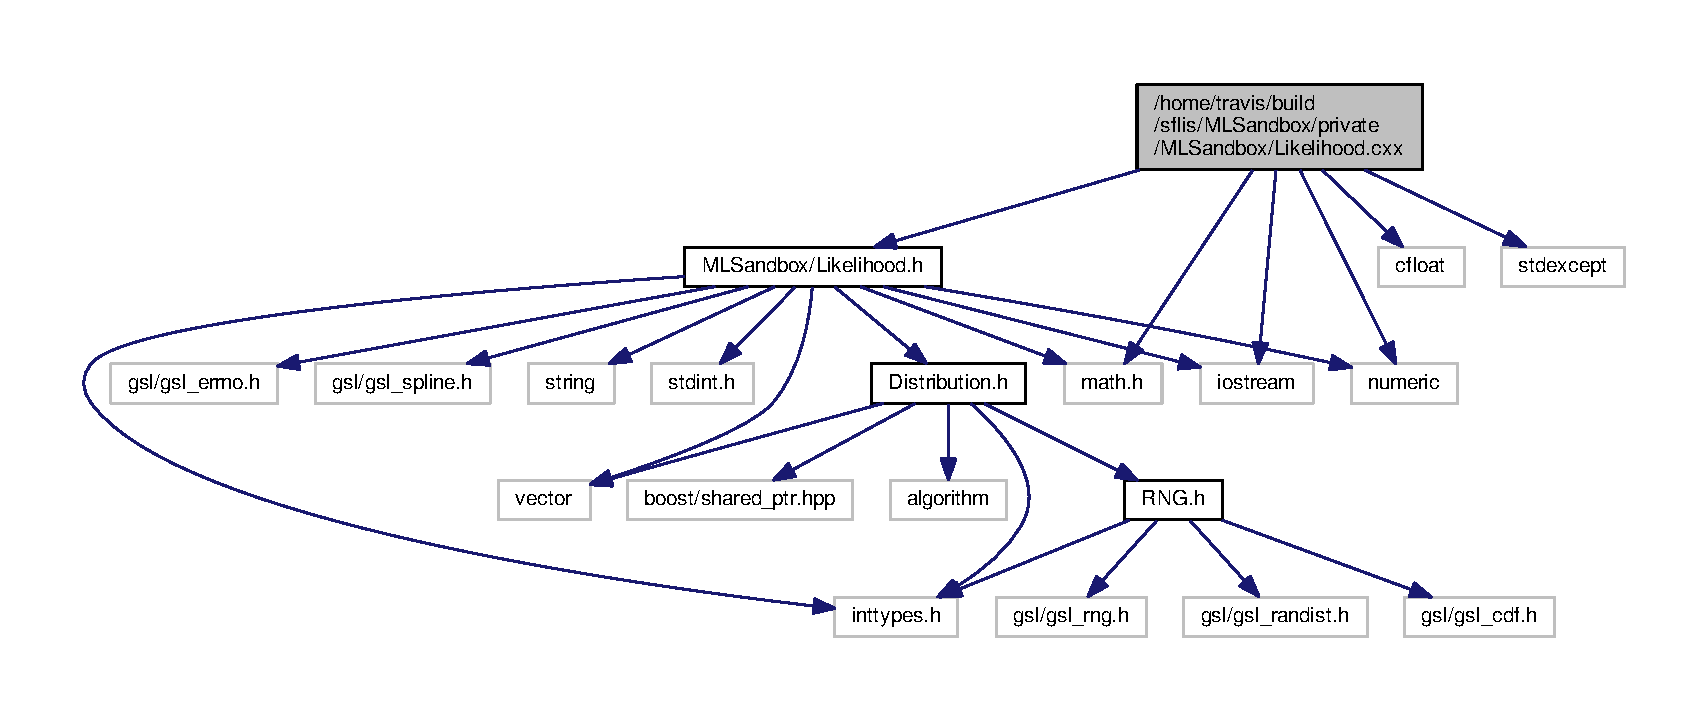
\includegraphics[width=350pt]{MLSandbox_2Likelihood_8cxx__incl}
\end{center}
\end{figure}
\subsection*{Functions}
\begin{DoxyCompactItemize}
\item 
uint32\-\_\-t \hyperlink{MLSandbox_2Likelihood_8cxx_a11d69a8cb5ac90dfb13d2e25df8eb1ce}{Super\-Fast\-Hash} (const char $\ast$data, int len)
\end{DoxyCompactItemize}


\subsection{Function Documentation}
\hypertarget{MLSandbox_2Likelihood_8cxx_a11d69a8cb5ac90dfb13d2e25df8eb1ce}{\index{M\-L\-Sandbox/\-Likelihood.\-cxx@{M\-L\-Sandbox/\-Likelihood.\-cxx}!Super\-Fast\-Hash@{Super\-Fast\-Hash}}
\index{Super\-Fast\-Hash@{Super\-Fast\-Hash}!MLSandbox/Likelihood.cxx@{M\-L\-Sandbox/\-Likelihood.\-cxx}}
\subsubsection[{Super\-Fast\-Hash}]{\setlength{\rightskip}{0pt plus 5cm}uint32\-\_\-t Super\-Fast\-Hash (
\begin{DoxyParamCaption}
\item[{const char $\ast$}]{data, }
\item[{int}]{len}
\end{DoxyParamCaption}
)}}\label{MLSandbox_2Likelihood_8cxx_a11d69a8cb5ac90dfb13d2e25df8eb1ce}

\hypertarget{pybindings_2Likelihood_8cxx}{\section{/home/travis/build/sflis/\-M\-L\-Sandbox/private/pybindings/\-Likelihood.cxx File Reference}
\label{pybindings_2Likelihood_8cxx}\index{/home/travis/build/sflis/\-M\-L\-Sandbox/private/pybindings/\-Likelihood.\-cxx@{/home/travis/build/sflis/\-M\-L\-Sandbox/private/pybindings/\-Likelihood.\-cxx}}
}
{\ttfamily \#include \char`\"{}M\-L\-Sandbox/\-Likelihood.\-h\char`\"{}}\\*
{\ttfamily \#include \char`\"{}M\-L\-Sandbox/\-Distribution.\-h\char`\"{}}\\*
{\ttfamily \#include \char`\"{}M\-L\-Sandbox/\-Combined\-Likelihood.\-h\char`\"{}}\\*
{\ttfamily \#include \char`\"{}M\-L\-Sandbox/\-Signal\-Contaminated\-L\-H.\-h\char`\"{}}\\*
{\ttfamily \#include \char`\"{}M\-L\-Sandbox/\-Likelihood\-Collection.\-h\char`\"{}}\\*
{\ttfamily \#include \char`\"{}bindingutils.\-h\char`\"{}}\\*
{\ttfamily \#include $<$boost/python.\-hpp$>$}\\*
{\ttfamily \#include $<$boost/python/tuple.\-hpp$>$}\\*
{\ttfamily \#include $<$boost/python/module.\-hpp$>$}\\*
{\ttfamily \#include $<$boost/python/def.\-hpp$>$}\\*
{\ttfamily \#include $<$boost/python/class.\-hpp$>$}\\*
{\ttfamily \#include $<$boost/python/dict.\-hpp$>$}\\*
{\ttfamily \#include $<$boost/numpy.\-hpp$>$}\\*
{\ttfamily \#include $<$numpy/arrayobject.\-h$>$}\\*
Include dependency graph for Likelihood.\-cxx\-:
\nopagebreak
\begin{figure}[H]
\begin{center}
\leavevmode
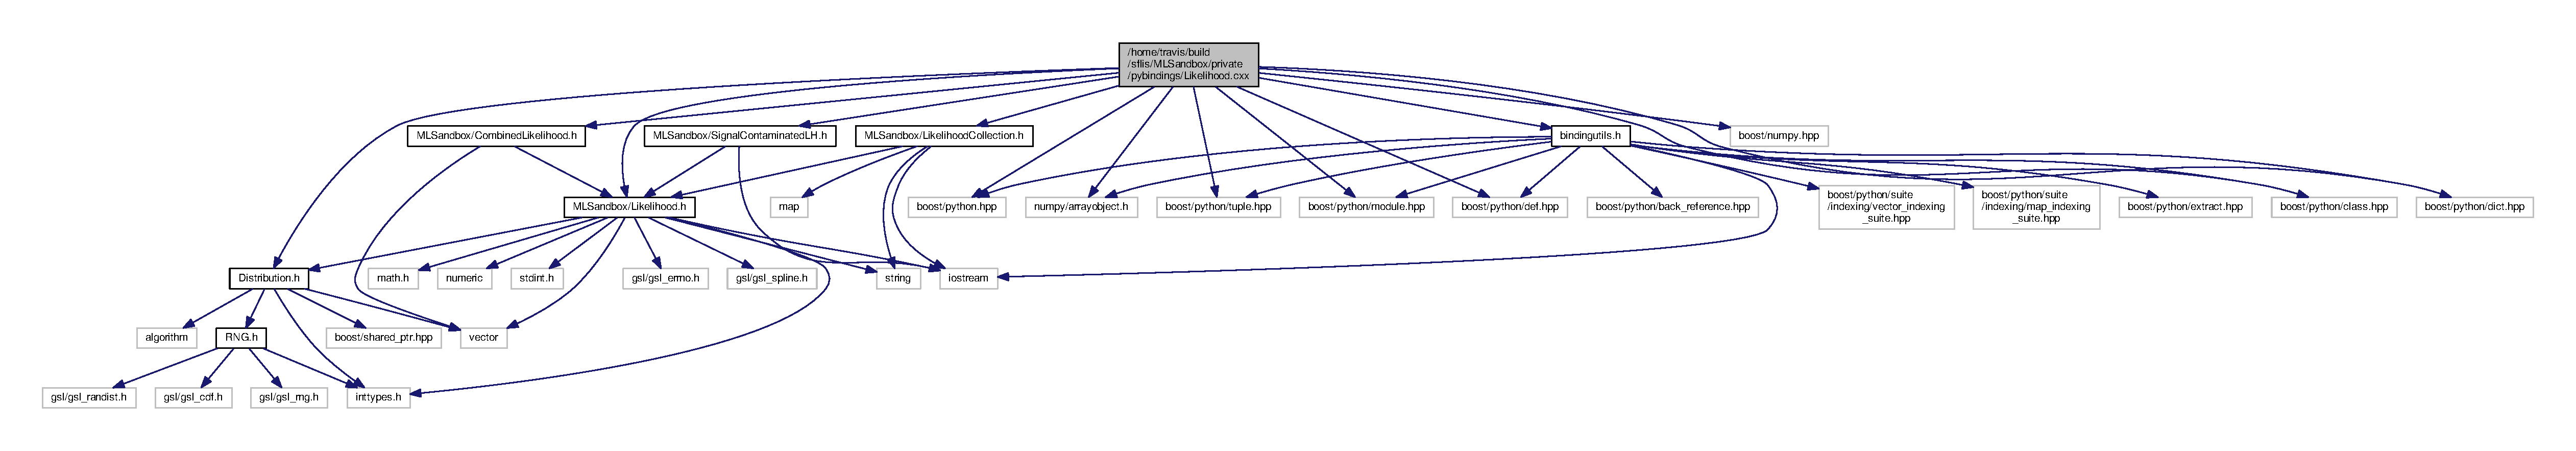
\includegraphics[width=350pt]{pybindings_2Likelihood_8cxx__incl}
\end{center}
\end{figure}
\subsection*{Namespaces}
\begin{DoxyCompactItemize}
\item 
\hyperlink{namespacemlsandbox}{mlsandbox}
\item 
\hyperlink{namespacemlsandbox_1_1python}{mlsandbox\-::python}
\end{DoxyCompactItemize}
\subsection*{Macros}
\begin{DoxyCompactItemize}
\item 
\#define \hyperlink{pybindings_2Likelihood_8cxx_ab6e6ee86736f9ebb56e74ae21bf3ff8a}{N\-P\-Y\-\_\-\-N\-O\-\_\-\-D\-E\-P\-R\-E\-C\-A\-T\-E\-D\-\_\-\-A\-P\-I}~N\-P\-Y\-\_\-1\-\_\-7\-\_\-\-A\-P\-I\-\_\-\-V\-E\-R\-S\-I\-O\-N
\end{DoxyCompactItemize}
\subsection*{Functions}
\begin{DoxyCompactItemize}
\item 
bn\-::ndarray \hyperlink{namespacemlsandbox_1_1python_a34e7315520ddd52ff2425944ff0b7ceb}{mlsandbox\-::python\-::get\-\_\-events} (\hyperlink{classBinnedLikelihood}{Binned\-Likelihood} \&self)
\item 
void \hyperlink{namespacemlsandbox_1_1python_a2b76c3fcdec9f6639cf79a73939c63a2}{mlsandbox\-::python\-::set\-\_\-events} (\hyperlink{classBinnedLikelihood}{Binned\-Likelihood} \&self, bp\-::object obj)
\item 
boost\-::shared\-\_\-ptr\\*
$<$ \hyperlink{classCombinedLikelihood}{Combined\-Likelihood} $>$ \hyperlink{namespacemlsandbox_1_1python_a1e62411a6ea1b3d42e90559d5537ceb6}{mlsandbox\-::python\-::init\-Wrapper\-Combined\-Likelihood} (bp\-::object const \&l\-\_\-list, bp\-::object const \&w\-\_\-list)
\item 
void \hyperlink{pybindings_2Likelihood_8cxx_a4dc0bafec23bc1ae4727f0921ddb34c7}{register\-\_\-\-Likelihood} ()
\end{DoxyCompactItemize}


\subsection{Macro Definition Documentation}
\hypertarget{pybindings_2Likelihood_8cxx_ab6e6ee86736f9ebb56e74ae21bf3ff8a}{\index{pybindings/\-Likelihood.\-cxx@{pybindings/\-Likelihood.\-cxx}!N\-P\-Y\-\_\-\-N\-O\-\_\-\-D\-E\-P\-R\-E\-C\-A\-T\-E\-D\-\_\-\-A\-P\-I@{N\-P\-Y\-\_\-\-N\-O\-\_\-\-D\-E\-P\-R\-E\-C\-A\-T\-E\-D\-\_\-\-A\-P\-I}}
\index{N\-P\-Y\-\_\-\-N\-O\-\_\-\-D\-E\-P\-R\-E\-C\-A\-T\-E\-D\-\_\-\-A\-P\-I@{N\-P\-Y\-\_\-\-N\-O\-\_\-\-D\-E\-P\-R\-E\-C\-A\-T\-E\-D\-\_\-\-A\-P\-I}!pybindings/Likelihood.cxx@{pybindings/\-Likelihood.\-cxx}}
\subsubsection[{N\-P\-Y\-\_\-\-N\-O\-\_\-\-D\-E\-P\-R\-E\-C\-A\-T\-E\-D\-\_\-\-A\-P\-I}]{\setlength{\rightskip}{0pt plus 5cm}\#define N\-P\-Y\-\_\-\-N\-O\-\_\-\-D\-E\-P\-R\-E\-C\-A\-T\-E\-D\-\_\-\-A\-P\-I~N\-P\-Y\-\_\-1\-\_\-7\-\_\-\-A\-P\-I\-\_\-\-V\-E\-R\-S\-I\-O\-N}}\label{pybindings_2Likelihood_8cxx_ab6e6ee86736f9ebb56e74ae21bf3ff8a}


\subsection{Function Documentation}
\hypertarget{pybindings_2Likelihood_8cxx_a4dc0bafec23bc1ae4727f0921ddb34c7}{\index{pybindings/\-Likelihood.\-cxx@{pybindings/\-Likelihood.\-cxx}!register\-\_\-\-Likelihood@{register\-\_\-\-Likelihood}}
\index{register\-\_\-\-Likelihood@{register\-\_\-\-Likelihood}!pybindings/Likelihood.cxx@{pybindings/\-Likelihood.\-cxx}}
\subsubsection[{register\-\_\-\-Likelihood}]{\setlength{\rightskip}{0pt plus 5cm}void register\-\_\-\-Likelihood (
\begin{DoxyParamCaption}
{}
\end{DoxyParamCaption}
)}}\label{pybindings_2Likelihood_8cxx_a4dc0bafec23bc1ae4727f0921ddb34c7}

\hypertarget{LikelihoodCollection_8cxx}{\section{/home/travis/build/sflis/\-M\-L\-Sandbox/private/\-M\-L\-Sandbox/\-Likelihood\-Collection.cxx File Reference}
\label{LikelihoodCollection_8cxx}\index{/home/travis/build/sflis/\-M\-L\-Sandbox/private/\-M\-L\-Sandbox/\-Likelihood\-Collection.\-cxx@{/home/travis/build/sflis/\-M\-L\-Sandbox/private/\-M\-L\-Sandbox/\-Likelihood\-Collection.\-cxx}}
}
{\ttfamily \#include \char`\"{}M\-L\-Sandbox/\-Likelihood\-Collection.\-h\char`\"{}}\\*
{\ttfamily \#include \char`\"{}M\-L\-Sandbox/\-Minimizer.\-h\char`\"{}}\\*
{\ttfamily \#include $<$math.\-h$>$}\\*
{\ttfamily \#include $<$iostream$>$}\\*
{\ttfamily \#include $<$cfloat$>$}\\*
{\ttfamily \#include $<$numeric$>$}\\*
{\ttfamily \#include $<$stdexcept$>$}\\*
{\ttfamily \#include $<$limits$>$}\\*
Include dependency graph for Likelihood\-Collection.\-cxx\-:
\nopagebreak
\begin{figure}[H]
\begin{center}
\leavevmode
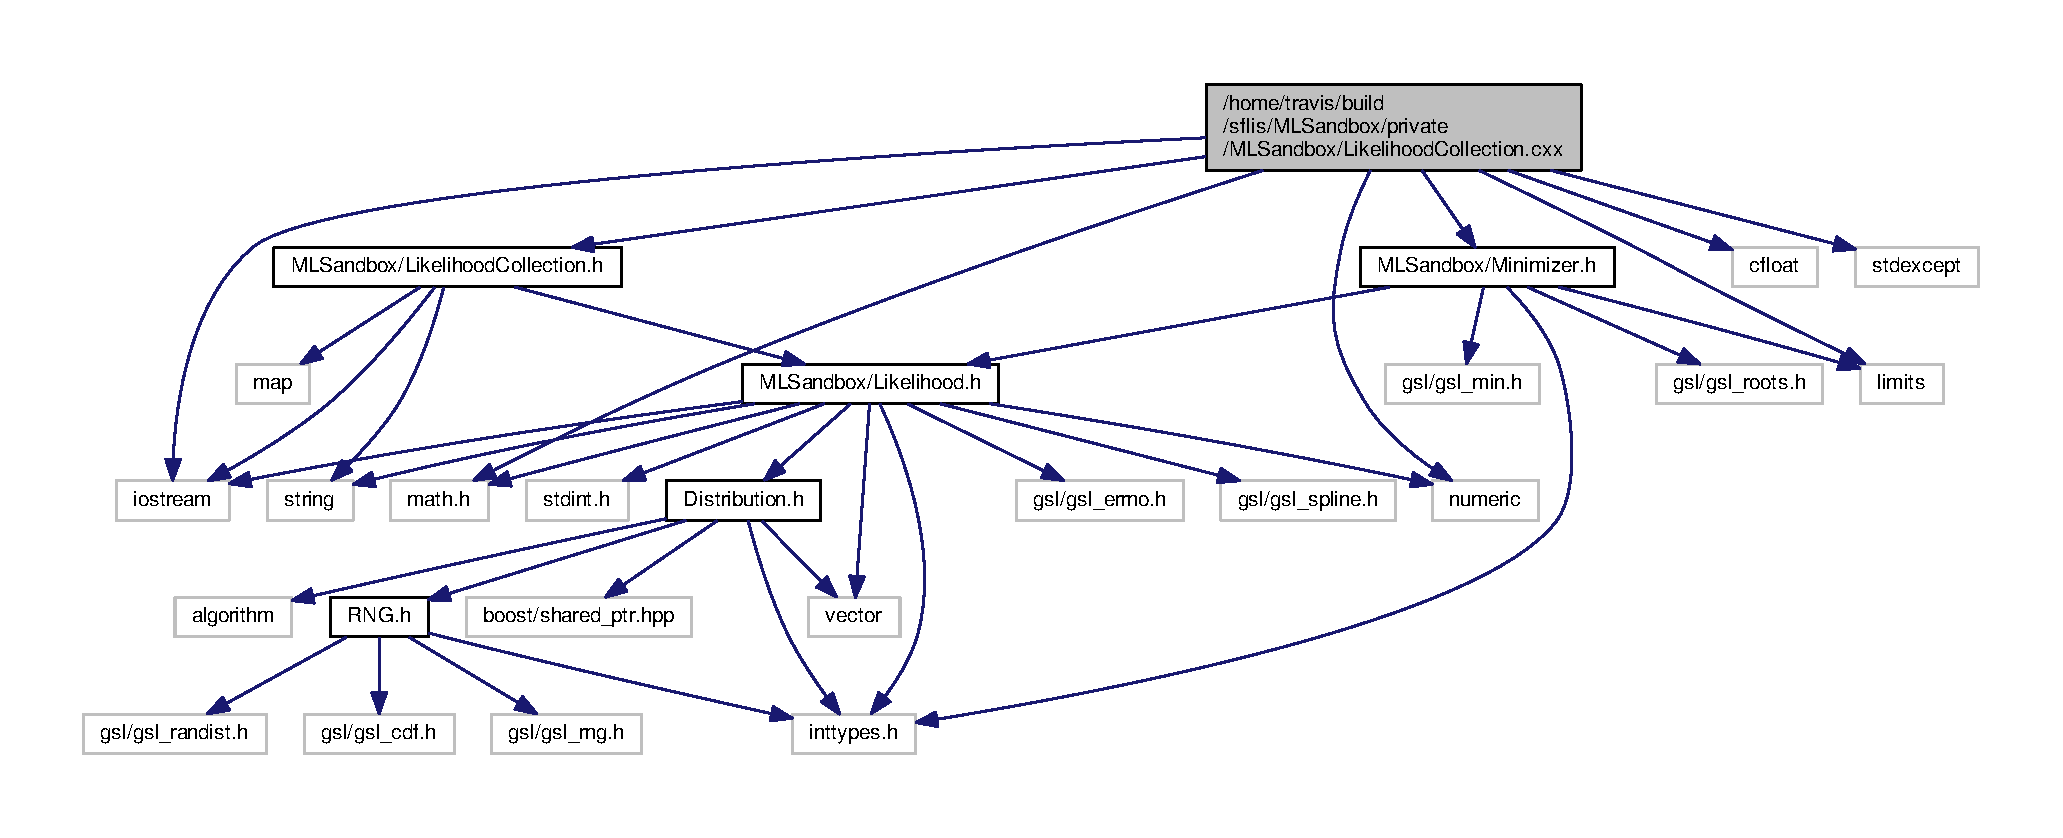
\includegraphics[width=350pt]{LikelihoodCollection_8cxx__incl}
\end{center}
\end{figure}

\hypertarget{MLSandbox_2Minimizer_8cxx}{\section{/home/travis/build/sflis/\-M\-L\-Sandbox/private/\-M\-L\-Sandbox/\-Minimizer.cxx File Reference}
\label{MLSandbox_2Minimizer_8cxx}\index{/home/travis/build/sflis/\-M\-L\-Sandbox/private/\-M\-L\-Sandbox/\-Minimizer.\-cxx@{/home/travis/build/sflis/\-M\-L\-Sandbox/private/\-M\-L\-Sandbox/\-Minimizer.\-cxx}}
}
{\ttfamily \#include $<$gsl/gsl\-\_\-roots.\-h$>$}\\*
{\ttfamily \#include $<$gsl/gsl\-\_\-min.\-h$>$}\\*
{\ttfamily \#include $<$gsl/gsl\-\_\-errno.\-h$>$}\\*
{\ttfamily \#include $<$exception$>$}\\*
{\ttfamily \#include $<$stdexcept$>$}\\*
{\ttfamily \#include $<$stdio.\-h$>$}\\*
{\ttfamily \#include $<$cmath$>$}\\*
{\ttfamily \#include \char`\"{}M\-L\-Sandbox/\-Minimizer.\-h\char`\"{}}\\*
{\ttfamily \#include $<$iostream$>$}\\*
{\ttfamily \#include $<$string$>$}\\*
Include dependency graph for Minimizer.\-cxx\-:
\nopagebreak
\begin{figure}[H]
\begin{center}
\leavevmode
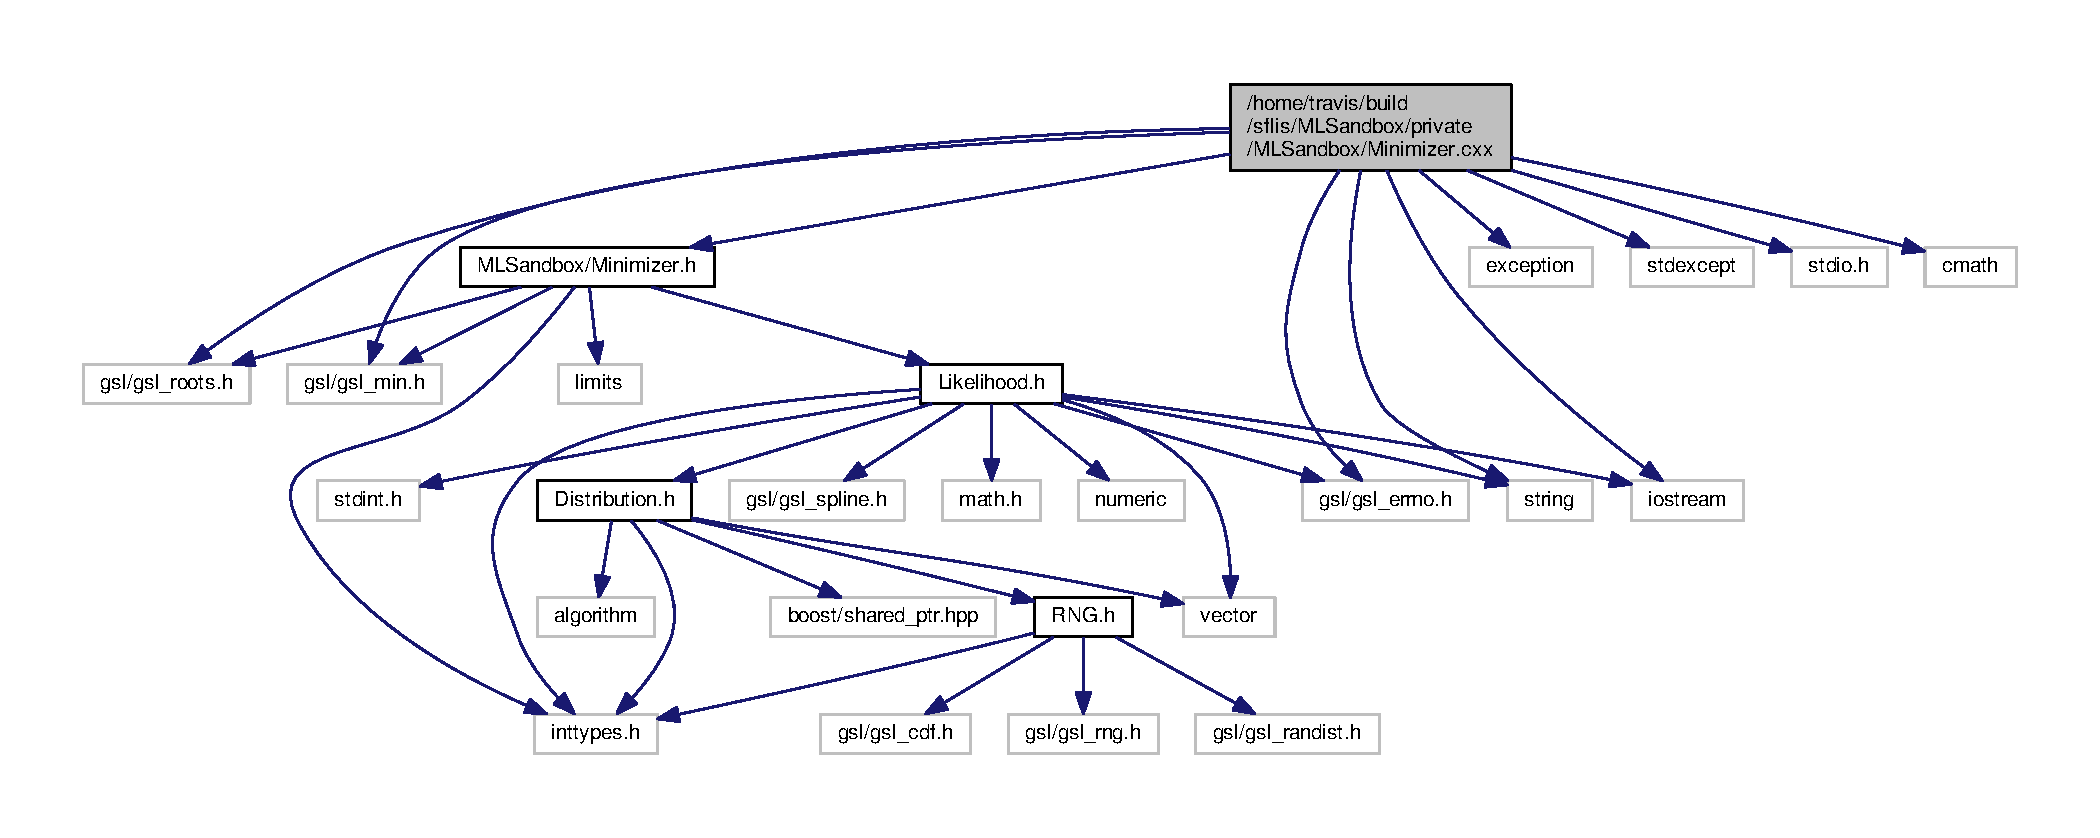
\includegraphics[width=350pt]{MLSandbox_2Minimizer_8cxx__incl}
\end{center}
\end{figure}

\hypertarget{pybindings_2Minimizer_8cxx}{\section{/home/travis/build/sflis/\-M\-L\-Sandbox/private/pybindings/\-Minimizer.cxx File Reference}
\label{pybindings_2Minimizer_8cxx}\index{/home/travis/build/sflis/\-M\-L\-Sandbox/private/pybindings/\-Minimizer.\-cxx@{/home/travis/build/sflis/\-M\-L\-Sandbox/private/pybindings/\-Minimizer.\-cxx}}
}
{\ttfamily \#include \char`\"{}M\-L\-Sandbox/\-Minimizer.\-h\char`\"{}}\\*
{\ttfamily \#include \char`\"{}bindingutils.\-h\char`\"{}}\\*
Include dependency graph for Minimizer.\-cxx\-:
\nopagebreak
\begin{figure}[H]
\begin{center}
\leavevmode
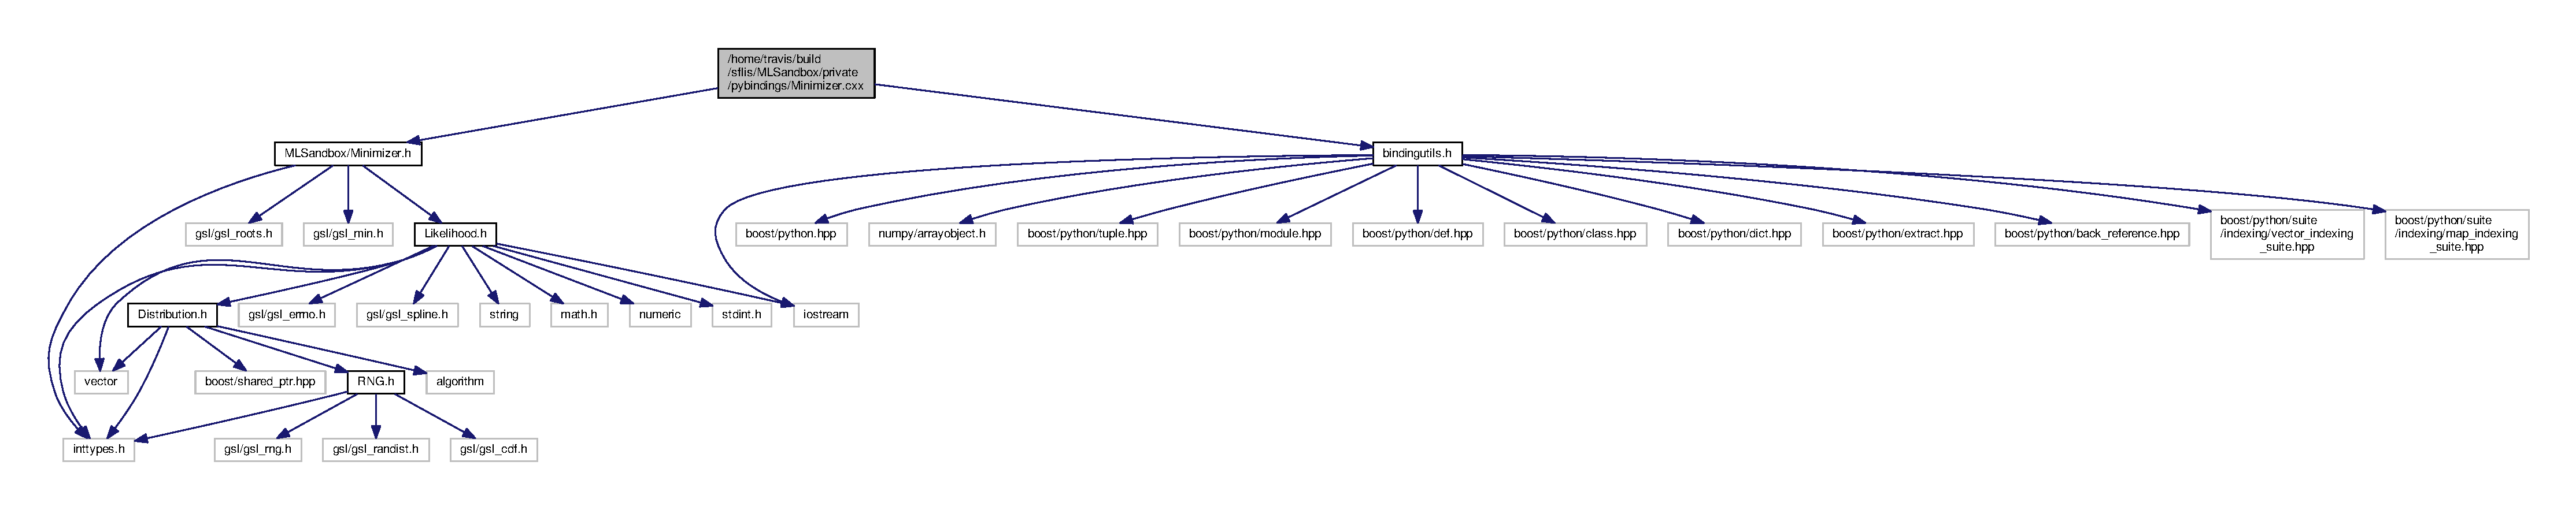
\includegraphics[width=350pt]{pybindings_2Minimizer_8cxx__incl}
\end{center}
\end{figure}
\subsection*{Macros}
\begin{DoxyCompactItemize}
\item 
\#define \hyperlink{pybindings_2Minimizer_8cxx_ab6e6ee86736f9ebb56e74ae21bf3ff8a}{N\-P\-Y\-\_\-\-N\-O\-\_\-\-D\-E\-P\-R\-E\-C\-A\-T\-E\-D\-\_\-\-A\-P\-I}~N\-P\-Y\-\_\-1\-\_\-7\-\_\-\-A\-P\-I\-\_\-\-V\-E\-R\-S\-I\-O\-N
\end{DoxyCompactItemize}
\subsection*{Functions}
\begin{DoxyCompactItemize}
\item 
void \hyperlink{pybindings_2Minimizer_8cxx_a9591cd1348c773742d2f63e8f8151e42}{register\-\_\-\-Minimizer} ()
\end{DoxyCompactItemize}


\subsection{Macro Definition Documentation}
\hypertarget{pybindings_2Minimizer_8cxx_ab6e6ee86736f9ebb56e74ae21bf3ff8a}{\index{pybindings/\-Minimizer.\-cxx@{pybindings/\-Minimizer.\-cxx}!N\-P\-Y\-\_\-\-N\-O\-\_\-\-D\-E\-P\-R\-E\-C\-A\-T\-E\-D\-\_\-\-A\-P\-I@{N\-P\-Y\-\_\-\-N\-O\-\_\-\-D\-E\-P\-R\-E\-C\-A\-T\-E\-D\-\_\-\-A\-P\-I}}
\index{N\-P\-Y\-\_\-\-N\-O\-\_\-\-D\-E\-P\-R\-E\-C\-A\-T\-E\-D\-\_\-\-A\-P\-I@{N\-P\-Y\-\_\-\-N\-O\-\_\-\-D\-E\-P\-R\-E\-C\-A\-T\-E\-D\-\_\-\-A\-P\-I}!pybindings/Minimizer.cxx@{pybindings/\-Minimizer.\-cxx}}
\subsubsection[{N\-P\-Y\-\_\-\-N\-O\-\_\-\-D\-E\-P\-R\-E\-C\-A\-T\-E\-D\-\_\-\-A\-P\-I}]{\setlength{\rightskip}{0pt plus 5cm}\#define N\-P\-Y\-\_\-\-N\-O\-\_\-\-D\-E\-P\-R\-E\-C\-A\-T\-E\-D\-\_\-\-A\-P\-I~N\-P\-Y\-\_\-1\-\_\-7\-\_\-\-A\-P\-I\-\_\-\-V\-E\-R\-S\-I\-O\-N}}\label{pybindings_2Minimizer_8cxx_ab6e6ee86736f9ebb56e74ae21bf3ff8a}


\subsection{Function Documentation}
\hypertarget{pybindings_2Minimizer_8cxx_a9591cd1348c773742d2f63e8f8151e42}{\index{pybindings/\-Minimizer.\-cxx@{pybindings/\-Minimizer.\-cxx}!register\-\_\-\-Minimizer@{register\-\_\-\-Minimizer}}
\index{register\-\_\-\-Minimizer@{register\-\_\-\-Minimizer}!pybindings/Minimizer.cxx@{pybindings/\-Minimizer.\-cxx}}
\subsubsection[{register\-\_\-\-Minimizer}]{\setlength{\rightskip}{0pt plus 5cm}void register\-\_\-\-Minimizer (
\begin{DoxyParamCaption}
{}
\end{DoxyParamCaption}
)}}\label{pybindings_2Minimizer_8cxx_a9591cd1348c773742d2f63e8f8151e42}

\hypertarget{MLSandbox_2NeymanAnalysis_8cxx}{\section{/home/travis/build/sflis/\-M\-L\-Sandbox/private/\-M\-L\-Sandbox/\-Neyman\-Analysis.cxx File Reference}
\label{MLSandbox_2NeymanAnalysis_8cxx}\index{/home/travis/build/sflis/\-M\-L\-Sandbox/private/\-M\-L\-Sandbox/\-Neyman\-Analysis.\-cxx@{/home/travis/build/sflis/\-M\-L\-Sandbox/private/\-M\-L\-Sandbox/\-Neyman\-Analysis.\-cxx}}
}
{\ttfamily \#include \char`\"{}M\-L\-Sandbox/\-Neyman\-Analysis.\-h\char`\"{}}\\*
{\ttfamily \#include \char`\"{}M\-L\-Sandbox/\-F\-C\-Ranks.\-h\char`\"{}}\\*
{\ttfamily \#include $<$gsl/gsl\-\_\-roots.\-h$>$}\\*
{\ttfamily \#include $<$gsl/gsl\-\_\-min.\-h$>$}\\*
{\ttfamily \#include $<$pthread.\-h$>$}\\*
{\ttfamily \#include $<$string$>$}\\*
{\ttfamily \#include $<$iostream$>$}\\*
{\ttfamily \#include $<$iomanip$>$}\\*
{\ttfamily \#include $<$algorithm$>$}\\*
{\ttfamily \#include $<$queue$>$}\\*
{\ttfamily \#include $<$boost/make\-\_\-shared.\-hpp$>$}\\*
Include dependency graph for Neyman\-Analysis.\-cxx\-:
\nopagebreak
\begin{figure}[H]
\begin{center}
\leavevmode
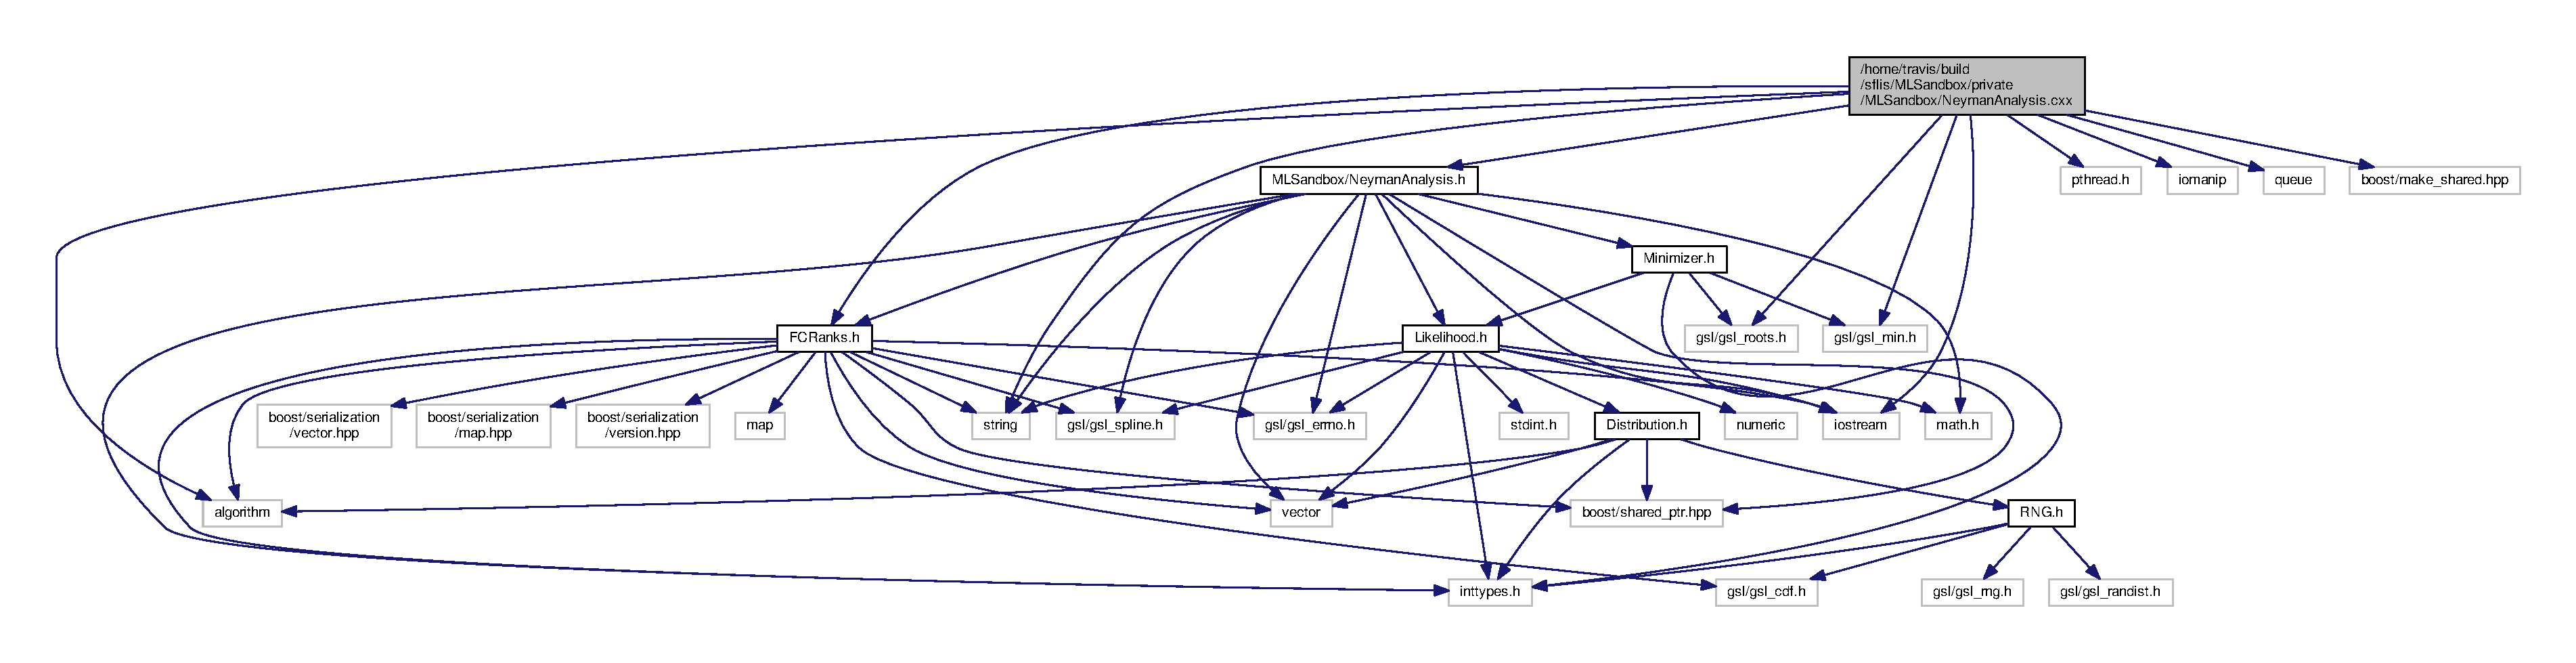
\includegraphics[width=350pt]{MLSandbox_2NeymanAnalysis_8cxx__incl}
\end{center}
\end{figure}
\subsection*{Classes}
\begin{DoxyCompactItemize}
\item 
struct \hyperlink{structNeymanThreadData}{Neyman\-Thread\-Data}
\item 
struct \hyperlink{structjob}{job}
\end{DoxyCompactItemize}
\subsection*{Functions}
\begin{DoxyCompactItemize}
\item 
void $\ast$ \hyperlink{MLSandbox_2NeymanAnalysis_8cxx_adc09985cd0b67a4c7928897809a69a46}{ts\-Computation\-Thread} (void $\ast$data)
\end{DoxyCompactItemize}
\subsection*{Variables}
\begin{DoxyCompactItemize}
\item 
pthread\-\_\-mutex\-\_\-t \hyperlink{MLSandbox_2NeymanAnalysis_8cxx_a8abebecb90f7a06f74188d978993ec50}{mutex\-Neyman\-Fetch\-Hypothesis} = P\-T\-H\-R\-E\-A\-D\-\_\-\-M\-U\-T\-E\-X\-\_\-\-I\-N\-I\-T\-I\-A\-L\-I\-Z\-E\-R
\item 
pthread\-\_\-mutex\-\_\-t \hyperlink{MLSandbox_2NeymanAnalysis_8cxx_a73c8f36839d409c2ed5e2fe8d3e2e377}{mutex\-Neyman\-Write\-Ranks} = P\-T\-H\-R\-E\-A\-D\-\_\-\-M\-U\-T\-E\-X\-\_\-\-I\-N\-I\-T\-I\-A\-L\-I\-Z\-E\-R
\end{DoxyCompactItemize}


\subsection{Function Documentation}
\hypertarget{MLSandbox_2NeymanAnalysis_8cxx_adc09985cd0b67a4c7928897809a69a46}{\index{M\-L\-Sandbox/\-Neyman\-Analysis.\-cxx@{M\-L\-Sandbox/\-Neyman\-Analysis.\-cxx}!ts\-Computation\-Thread@{ts\-Computation\-Thread}}
\index{ts\-Computation\-Thread@{ts\-Computation\-Thread}!MLSandbox/NeymanAnalysis.cxx@{M\-L\-Sandbox/\-Neyman\-Analysis.\-cxx}}
\subsubsection[{ts\-Computation\-Thread}]{\setlength{\rightskip}{0pt plus 5cm}void $\ast$ ts\-Computation\-Thread (
\begin{DoxyParamCaption}
\item[{void $\ast$}]{data}
\end{DoxyParamCaption}
)}}\label{MLSandbox_2NeymanAnalysis_8cxx_adc09985cd0b67a4c7928897809a69a46}


\subsection{Variable Documentation}
\hypertarget{MLSandbox_2NeymanAnalysis_8cxx_a8abebecb90f7a06f74188d978993ec50}{\index{M\-L\-Sandbox/\-Neyman\-Analysis.\-cxx@{M\-L\-Sandbox/\-Neyman\-Analysis.\-cxx}!mutex\-Neyman\-Fetch\-Hypothesis@{mutex\-Neyman\-Fetch\-Hypothesis}}
\index{mutex\-Neyman\-Fetch\-Hypothesis@{mutex\-Neyman\-Fetch\-Hypothesis}!MLSandbox/NeymanAnalysis.cxx@{M\-L\-Sandbox/\-Neyman\-Analysis.\-cxx}}
\subsubsection[{mutex\-Neyman\-Fetch\-Hypothesis}]{\setlength{\rightskip}{0pt plus 5cm}pthread\-\_\-mutex\-\_\-t mutex\-Neyman\-Fetch\-Hypothesis = P\-T\-H\-R\-E\-A\-D\-\_\-\-M\-U\-T\-E\-X\-\_\-\-I\-N\-I\-T\-I\-A\-L\-I\-Z\-E\-R}}\label{MLSandbox_2NeymanAnalysis_8cxx_a8abebecb90f7a06f74188d978993ec50}
\hypertarget{MLSandbox_2NeymanAnalysis_8cxx_a73c8f36839d409c2ed5e2fe8d3e2e377}{\index{M\-L\-Sandbox/\-Neyman\-Analysis.\-cxx@{M\-L\-Sandbox/\-Neyman\-Analysis.\-cxx}!mutex\-Neyman\-Write\-Ranks@{mutex\-Neyman\-Write\-Ranks}}
\index{mutex\-Neyman\-Write\-Ranks@{mutex\-Neyman\-Write\-Ranks}!MLSandbox/NeymanAnalysis.cxx@{M\-L\-Sandbox/\-Neyman\-Analysis.\-cxx}}
\subsubsection[{mutex\-Neyman\-Write\-Ranks}]{\setlength{\rightskip}{0pt plus 5cm}pthread\-\_\-mutex\-\_\-t mutex\-Neyman\-Write\-Ranks = P\-T\-H\-R\-E\-A\-D\-\_\-\-M\-U\-T\-E\-X\-\_\-\-I\-N\-I\-T\-I\-A\-L\-I\-Z\-E\-R}}\label{MLSandbox_2NeymanAnalysis_8cxx_a73c8f36839d409c2ed5e2fe8d3e2e377}

\hypertarget{pybindings_2NeymanAnalysis_8cxx}{\section{/home/travis/build/sflis/\-M\-L\-Sandbox/private/pybindings/\-Neyman\-Analysis.cxx File Reference}
\label{pybindings_2NeymanAnalysis_8cxx}\index{/home/travis/build/sflis/\-M\-L\-Sandbox/private/pybindings/\-Neyman\-Analysis.\-cxx@{/home/travis/build/sflis/\-M\-L\-Sandbox/private/pybindings/\-Neyman\-Analysis.\-cxx}}
}
{\ttfamily \#include \char`\"{}M\-L\-Sandbox/\-Neyman\-Analysis.\-h\char`\"{}}\\*
{\ttfamily \#include $<$boost/numpy.\-hpp$>$}\\*
{\ttfamily \#include $<$boost/python/tuple.\-hpp$>$}\\*
{\ttfamily \#include $<$iostream$>$}\\*
{\ttfamily \#include $<$vector$>$}\\*
Include dependency graph for Neyman\-Analysis.\-cxx\-:
\nopagebreak
\begin{figure}[H]
\begin{center}
\leavevmode
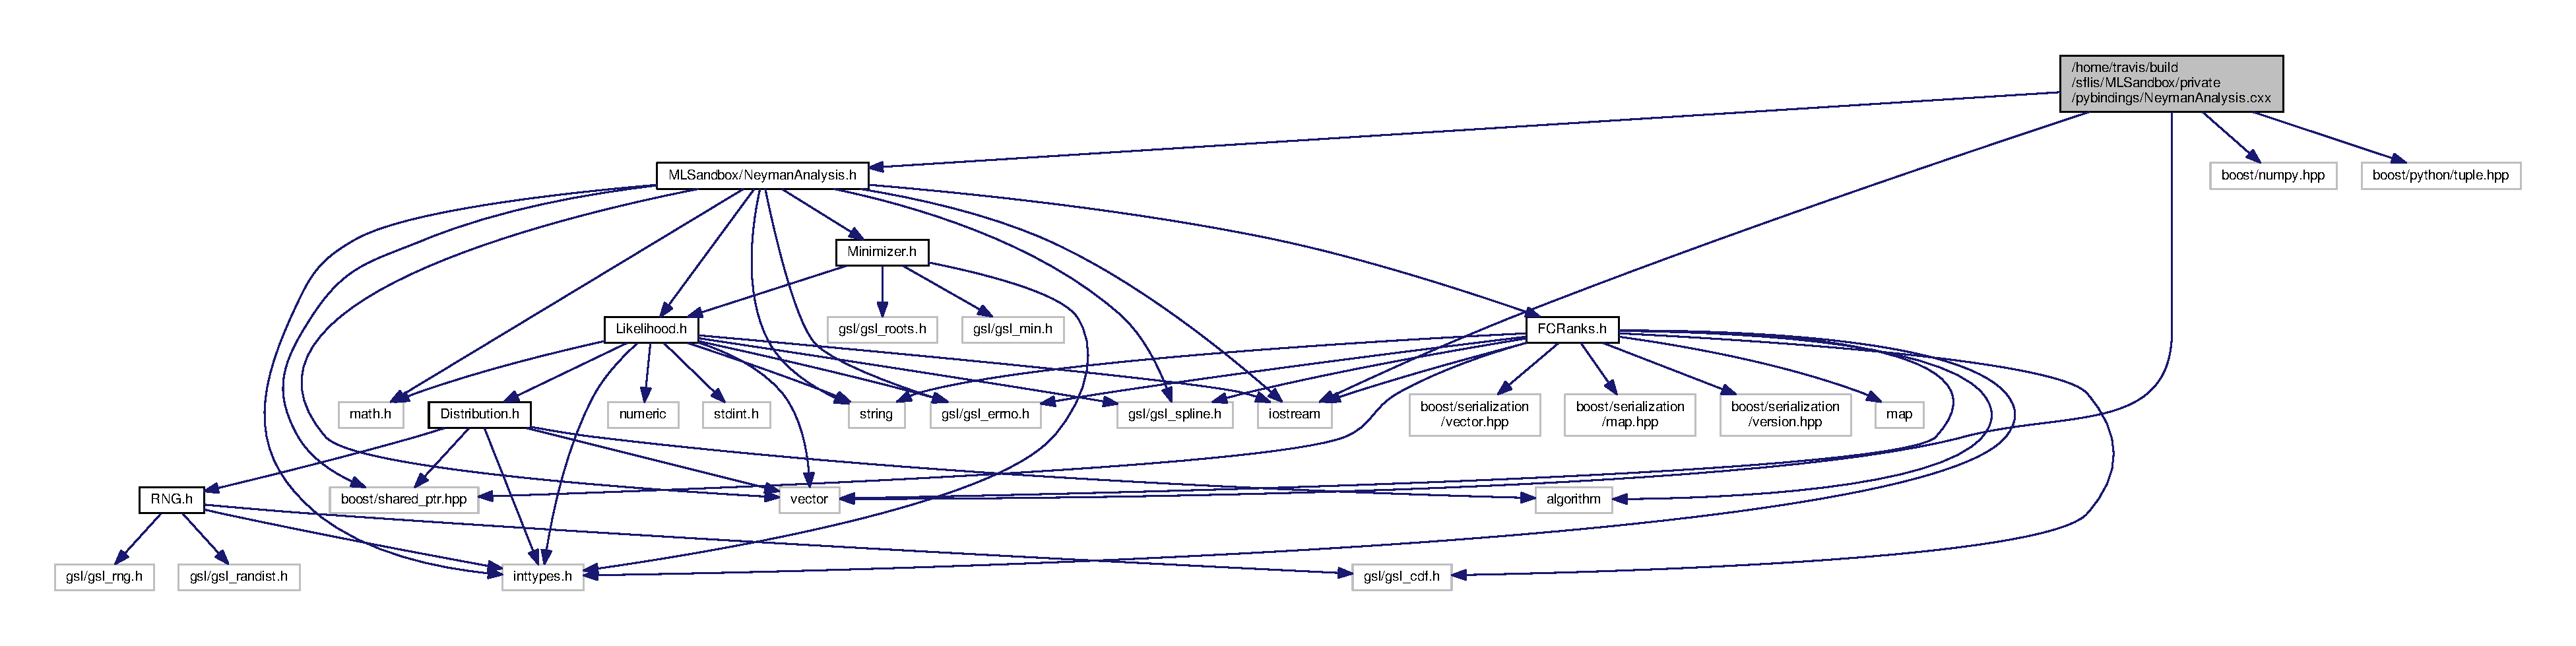
\includegraphics[width=350pt]{pybindings_2NeymanAnalysis_8cxx__incl}
\end{center}
\end{figure}
\subsection*{Namespaces}
\begin{DoxyCompactItemize}
\item 
\hyperlink{namespacemlsandbox}{mlsandbox}
\end{DoxyCompactItemize}
\subsection*{Functions}
\begin{DoxyCompactItemize}
\item 
void \hyperlink{pybindings_2NeymanAnalysis_8cxx_a48f35108bf6e823923f20275fa1183a3}{register\-\_\-\-Neyman\-Analysis} ()
\end{DoxyCompactItemize}


\subsection{Function Documentation}
\hypertarget{pybindings_2NeymanAnalysis_8cxx_a48f35108bf6e823923f20275fa1183a3}{\index{pybindings/\-Neyman\-Analysis.\-cxx@{pybindings/\-Neyman\-Analysis.\-cxx}!register\-\_\-\-Neyman\-Analysis@{register\-\_\-\-Neyman\-Analysis}}
\index{register\-\_\-\-Neyman\-Analysis@{register\-\_\-\-Neyman\-Analysis}!pybindings/NeymanAnalysis.cxx@{pybindings/\-Neyman\-Analysis.\-cxx}}
\subsubsection[{register\-\_\-\-Neyman\-Analysis}]{\setlength{\rightskip}{0pt plus 5cm}void register\-\_\-\-Neyman\-Analysis (
\begin{DoxyParamCaption}
{}
\end{DoxyParamCaption}
)}}\label{pybindings_2NeymanAnalysis_8cxx_a48f35108bf6e823923f20275fa1183a3}

\hypertarget{SignalContaminatedLH_8cxx}{\section{/home/travis/build/sflis/\-M\-L\-Sandbox/private/\-M\-L\-Sandbox/\-Signal\-Contaminated\-L\-H.cxx File Reference}
\label{SignalContaminatedLH_8cxx}\index{/home/travis/build/sflis/\-M\-L\-Sandbox/private/\-M\-L\-Sandbox/\-Signal\-Contaminated\-L\-H.\-cxx@{/home/travis/build/sflis/\-M\-L\-Sandbox/private/\-M\-L\-Sandbox/\-Signal\-Contaminated\-L\-H.\-cxx}}
}
{\ttfamily \#include \char`\"{}M\-L\-Sandbox/\-Signal\-Contaminated\-L\-H.\-h\char`\"{}}\\*
{\ttfamily \#include \char`\"{}M\-L\-Sandbox/\-Minimizer.\-h\char`\"{}}\\*
{\ttfamily \#include $<$math.\-h$>$}\\*
{\ttfamily \#include $<$iostream$>$}\\*
{\ttfamily \#include $<$cfloat$>$}\\*
{\ttfamily \#include $<$numeric$>$}\\*
{\ttfamily \#include $<$stdexcept$>$}\\*
{\ttfamily \#include $<$limits$>$}\\*
Include dependency graph for Signal\-Contaminated\-L\-H.\-cxx\-:
\nopagebreak
\begin{figure}[H]
\begin{center}
\leavevmode
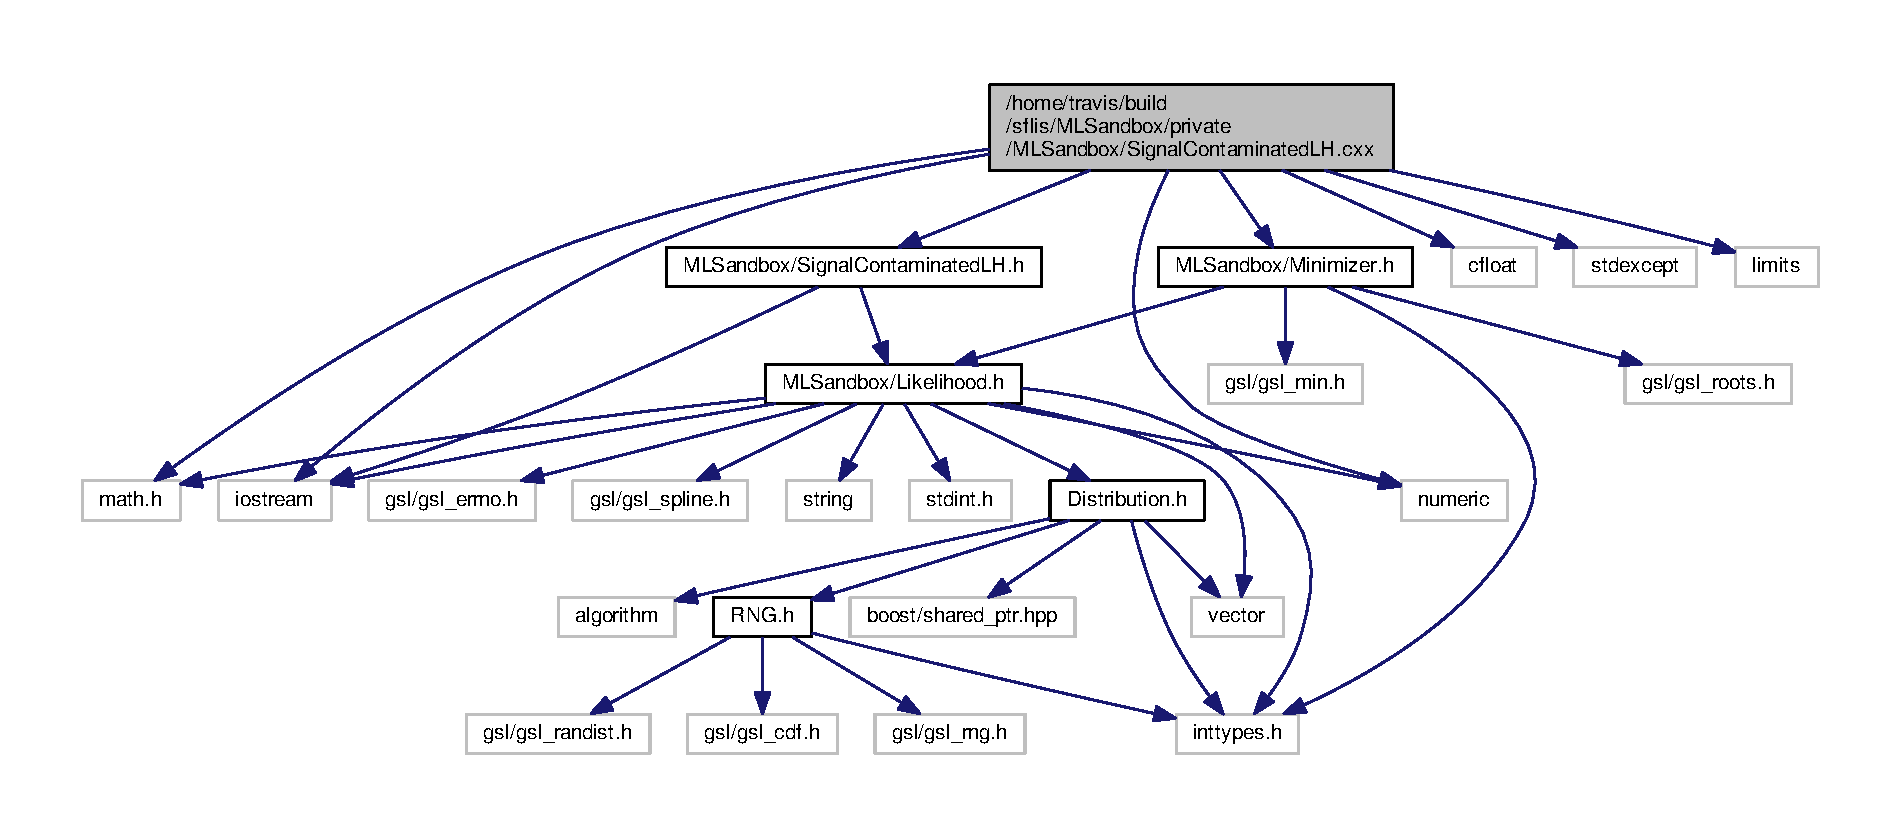
\includegraphics[width=350pt]{SignalContaminatedLH_8cxx__incl}
\end{center}
\end{figure}

\hypertarget{bindingutils_8h}{\section{/home/travis/build/sflis/\-M\-L\-Sandbox/private/pybindings/bindingutils.h File Reference}
\label{bindingutils_8h}\index{/home/travis/build/sflis/\-M\-L\-Sandbox/private/pybindings/bindingutils.\-h@{/home/travis/build/sflis/\-M\-L\-Sandbox/private/pybindings/bindingutils.\-h}}
}
{\ttfamily \#include $<$boost/python.\-hpp$>$}\\*
{\ttfamily \#include $<$numpy/arrayobject.\-h$>$}\\*
{\ttfamily \#include $<$boost/python/tuple.\-hpp$>$}\\*
{\ttfamily \#include $<$boost/python/module.\-hpp$>$}\\*
{\ttfamily \#include $<$boost/python/def.\-hpp$>$}\\*
{\ttfamily \#include $<$boost/python/class.\-hpp$>$}\\*
{\ttfamily \#include $<$boost/python/dict.\-hpp$>$}\\*
{\ttfamily \#include $<$boost/python/extract.\-hpp$>$}\\*
{\ttfamily \#include $<$boost/python/back\-\_\-reference.\-hpp$>$}\\*
{\ttfamily \#include $<$boost/python/suite/indexing/vector\-\_\-indexing\-\_\-suite.\-hpp$>$}\\*
{\ttfamily \#include $<$boost/python/suite/indexing/map\-\_\-indexing\-\_\-suite.\-hpp$>$}\\*
{\ttfamily \#include $<$iostream$>$}\\*
Include dependency graph for bindingutils.\-h\-:
\nopagebreak
\begin{figure}[H]
\begin{center}
\leavevmode
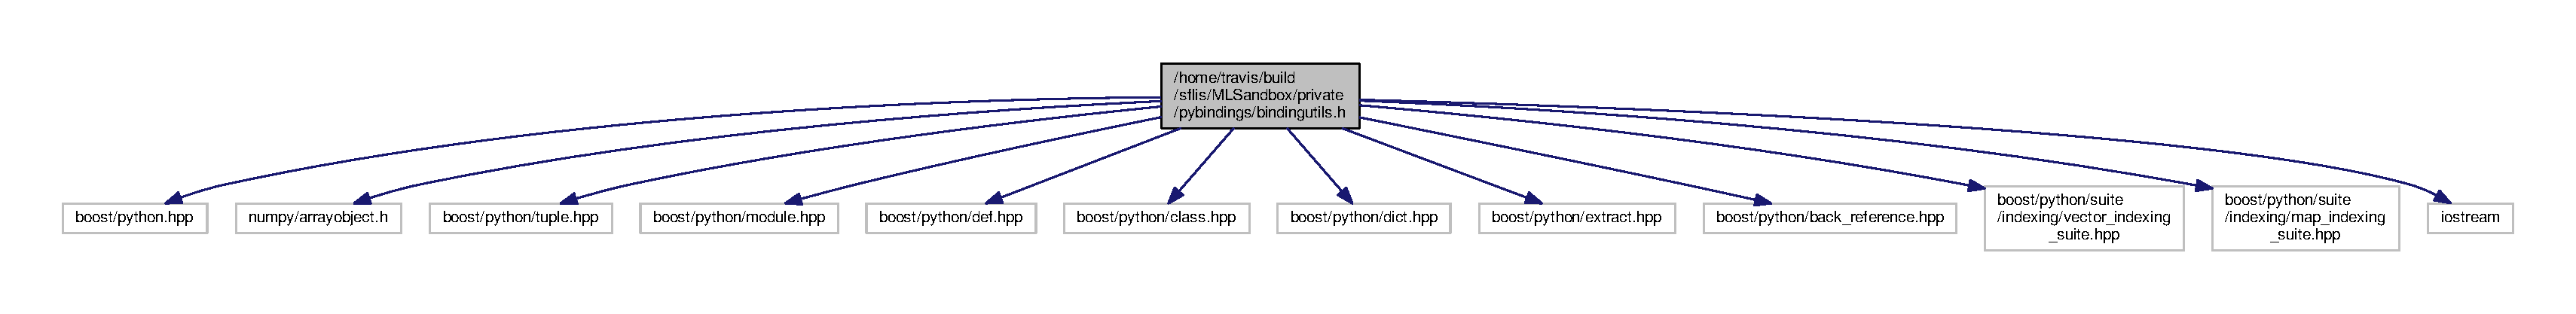
\includegraphics[width=350pt]{bindingutils_8h__incl}
\end{center}
\end{figure}
This graph shows which files directly or indirectly include this file\-:
\nopagebreak
\begin{figure}[H]
\begin{center}
\leavevmode
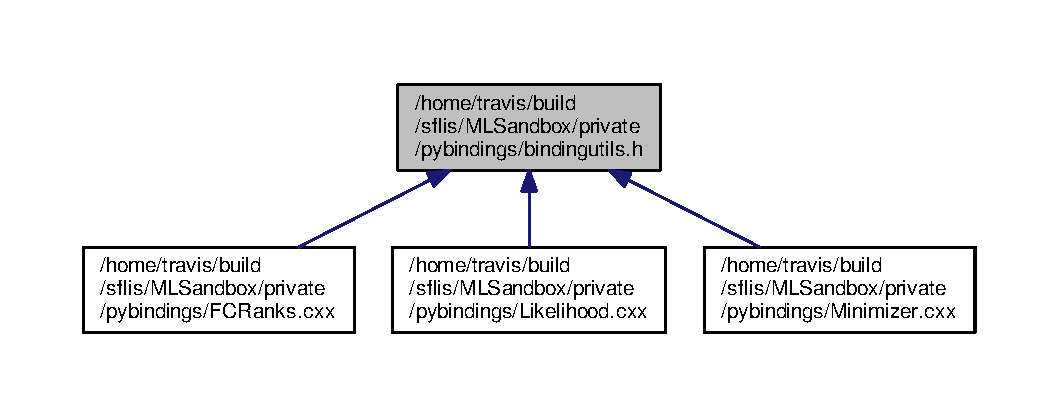
\includegraphics[width=350pt]{bindingutils_8h__dep__incl}
\end{center}
\end{figure}
\subsection*{Functions}
\begin{DoxyCompactItemize}
\item 
{\footnotesize template$<$class K , class V $>$ }\\boost\-::python\-::dict \hyperlink{bindingutils_8h_abeb1bc1a9d61a526987c14cfa99b5ca2}{to\-Python\-Dict} (const std\-::map$<$ K, V $>$ \&map)
\item 
{\footnotesize template$<$class K , class V $>$ }\\boost\-::python\-::dict \hyperlink{bindingutils_8h_ab86871a3baff796925aeece39712af7e}{to\-Python\-Dict} (const std\-::map$<$ K, std\-::vector$<$ V $>$ $>$ \&map)
\item 
{\footnotesize template$<$class V $>$ }\\boost\-::python\-::list \hyperlink{bindingutils_8h_a04867bd21ee2507d418f73c111d3af88}{to\-Python\-List} (const std\-::vector$<$ V $>$ \&vector)
\item 
{\footnotesize template$<$class K , class V $>$ }\\std\-::map$<$ K, V $>$ \hyperlink{bindingutils_8h_afecf56de807fcf0d676ae208e2d46f8f}{to\-Std\-Map} (boost\-::python\-::dict dictionary)
\item 
{\footnotesize template$<$class V $>$ }\\std\-::vector$<$ V $>$ \hyperlink{bindingutils_8h_ab5b9e0909c719546bdf6bf8cab3cdc17}{to\-Std\-Vector} (boost\-::python\-::list list)
\end{DoxyCompactItemize}


\subsection{Function Documentation}
\hypertarget{bindingutils_8h_abeb1bc1a9d61a526987c14cfa99b5ca2}{\index{bindingutils.\-h@{bindingutils.\-h}!to\-Python\-Dict@{to\-Python\-Dict}}
\index{to\-Python\-Dict@{to\-Python\-Dict}!bindingutils.h@{bindingutils.\-h}}
\subsubsection[{to\-Python\-Dict}]{\setlength{\rightskip}{0pt plus 5cm}template$<$class K , class V $>$ boost\-::python\-::dict to\-Python\-Dict (
\begin{DoxyParamCaption}
\item[{const std\-::map$<$ K, V $>$ \&}]{map}
\end{DoxyParamCaption}
)}}\label{bindingutils_8h_abeb1bc1a9d61a526987c14cfa99b5ca2}
\hypertarget{bindingutils_8h_ab86871a3baff796925aeece39712af7e}{\index{bindingutils.\-h@{bindingutils.\-h}!to\-Python\-Dict@{to\-Python\-Dict}}
\index{to\-Python\-Dict@{to\-Python\-Dict}!bindingutils.h@{bindingutils.\-h}}
\subsubsection[{to\-Python\-Dict}]{\setlength{\rightskip}{0pt plus 5cm}template$<$class K , class V $>$ boost\-::python\-::dict to\-Python\-Dict (
\begin{DoxyParamCaption}
\item[{const std\-::map$<$ K, std\-::vector$<$ V $>$ $>$ \&}]{map}
\end{DoxyParamCaption}
)}}\label{bindingutils_8h_ab86871a3baff796925aeece39712af7e}
\hypertarget{bindingutils_8h_a04867bd21ee2507d418f73c111d3af88}{\index{bindingutils.\-h@{bindingutils.\-h}!to\-Python\-List@{to\-Python\-List}}
\index{to\-Python\-List@{to\-Python\-List}!bindingutils.h@{bindingutils.\-h}}
\subsubsection[{to\-Python\-List}]{\setlength{\rightskip}{0pt plus 5cm}template$<$class V $>$ boost\-::python\-::list to\-Python\-List (
\begin{DoxyParamCaption}
\item[{const std\-::vector$<$ V $>$ \&}]{vector}
\end{DoxyParamCaption}
)}}\label{bindingutils_8h_a04867bd21ee2507d418f73c111d3af88}
\hypertarget{bindingutils_8h_afecf56de807fcf0d676ae208e2d46f8f}{\index{bindingutils.\-h@{bindingutils.\-h}!to\-Std\-Map@{to\-Std\-Map}}
\index{to\-Std\-Map@{to\-Std\-Map}!bindingutils.h@{bindingutils.\-h}}
\subsubsection[{to\-Std\-Map}]{\setlength{\rightskip}{0pt plus 5cm}template$<$class K , class V $>$ std\-::map$<$K, V$>$ to\-Std\-Map (
\begin{DoxyParamCaption}
\item[{boost\-::python\-::dict}]{dictionary}
\end{DoxyParamCaption}
)}}\label{bindingutils_8h_afecf56de807fcf0d676ae208e2d46f8f}
\hypertarget{bindingutils_8h_ab5b9e0909c719546bdf6bf8cab3cdc17}{\index{bindingutils.\-h@{bindingutils.\-h}!to\-Std\-Vector@{to\-Std\-Vector}}
\index{to\-Std\-Vector@{to\-Std\-Vector}!bindingutils.h@{bindingutils.\-h}}
\subsubsection[{to\-Std\-Vector}]{\setlength{\rightskip}{0pt plus 5cm}template$<$class V $>$ std\-::vector$<$V$>$ to\-Std\-Vector (
\begin{DoxyParamCaption}
\item[{boost\-::python\-::list}]{list}
\end{DoxyParamCaption}
)}}\label{bindingutils_8h_ab5b9e0909c719546bdf6bf8cab3cdc17}

\hypertarget{module_8cxx}{\section{/home/travis/build/sflis/\-M\-L\-Sandbox/private/pybindings/module.cxx File Reference}
\label{module_8cxx}\index{/home/travis/build/sflis/\-M\-L\-Sandbox/private/pybindings/module.\-cxx@{/home/travis/build/sflis/\-M\-L\-Sandbox/private/pybindings/module.\-cxx}}
}
{\ttfamily \#include $<$boost/preprocessor.\-hpp$>$}\\*
{\ttfamily \#include $<$boost/numpy.\-hpp$>$}\\*
Include dependency graph for module.\-cxx\-:
\nopagebreak
\begin{figure}[H]
\begin{center}
\leavevmode
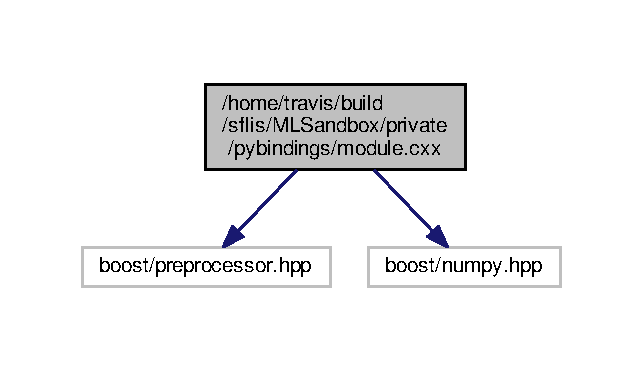
\includegraphics[width=309pt]{module_8cxx__incl}
\end{center}
\end{figure}
\subsection*{Macros}
\begin{DoxyCompactItemize}
\item 
\#define \hyperlink{module_8cxx_a7102a509156d26af75e87fb9c8bb9d50}{R\-E\-G\-I\-S\-T\-E\-R\-\_\-\-T\-H\-E\-S\-E\-\_\-\-T\-H\-I\-N\-G\-S}
\item 
\#define \hyperlink{module_8cxx_a0919ee25dec3a709f3ee57e614284e2a}{I3\-\_\-\-R\-E\-G\-I\-S\-T\-R\-A\-T\-I\-O\-N\-\_\-\-F\-N\-\_\-\-D\-E\-C\-L}(r, data, t)~void B\-O\-O\-S\-T\-\_\-\-P\-P\-\_\-\-C\-A\-T(register\-\_\-,t)();
\item 
\#define \hyperlink{module_8cxx_afa1bf5f2b0b65a4cfcb0d0c94540b612}{I3\-\_\-\-R\-E\-G\-I\-S\-T\-E\-R}(r, data, t)~B\-O\-O\-S\-T\-\_\-\-P\-P\-\_\-\-C\-A\-T(register\-\_\-,t)();
\end{DoxyCompactItemize}
\subsection*{Functions}
\begin{DoxyCompactItemize}
\item 
\hyperlink{module_8cxx_a571936a8bf585039bd56c829f54d39f1}{B\-O\-O\-S\-T\-\_\-\-P\-Y\-T\-H\-O\-N\-\_\-\-M\-O\-D\-U\-L\-E} (M\-L\-Sandbox)
\end{DoxyCompactItemize}


\subsection{Macro Definition Documentation}
\hypertarget{module_8cxx_afa1bf5f2b0b65a4cfcb0d0c94540b612}{\index{module.\-cxx@{module.\-cxx}!I3\-\_\-\-R\-E\-G\-I\-S\-T\-E\-R@{I3\-\_\-\-R\-E\-G\-I\-S\-T\-E\-R}}
\index{I3\-\_\-\-R\-E\-G\-I\-S\-T\-E\-R@{I3\-\_\-\-R\-E\-G\-I\-S\-T\-E\-R}!module.cxx@{module.\-cxx}}
\subsubsection[{I3\-\_\-\-R\-E\-G\-I\-S\-T\-E\-R}]{\setlength{\rightskip}{0pt plus 5cm}\#define I3\-\_\-\-R\-E\-G\-I\-S\-T\-E\-R(
\begin{DoxyParamCaption}
\item[{}]{r, }
\item[{}]{data, }
\item[{}]{t}
\end{DoxyParamCaption}
)~B\-O\-O\-S\-T\-\_\-\-P\-P\-\_\-\-C\-A\-T(register\-\_\-,t)();}}\label{module_8cxx_afa1bf5f2b0b65a4cfcb0d0c94540b612}
\hypertarget{module_8cxx_a0919ee25dec3a709f3ee57e614284e2a}{\index{module.\-cxx@{module.\-cxx}!I3\-\_\-\-R\-E\-G\-I\-S\-T\-R\-A\-T\-I\-O\-N\-\_\-\-F\-N\-\_\-\-D\-E\-C\-L@{I3\-\_\-\-R\-E\-G\-I\-S\-T\-R\-A\-T\-I\-O\-N\-\_\-\-F\-N\-\_\-\-D\-E\-C\-L}}
\index{I3\-\_\-\-R\-E\-G\-I\-S\-T\-R\-A\-T\-I\-O\-N\-\_\-\-F\-N\-\_\-\-D\-E\-C\-L@{I3\-\_\-\-R\-E\-G\-I\-S\-T\-R\-A\-T\-I\-O\-N\-\_\-\-F\-N\-\_\-\-D\-E\-C\-L}!module.cxx@{module.\-cxx}}
\subsubsection[{I3\-\_\-\-R\-E\-G\-I\-S\-T\-R\-A\-T\-I\-O\-N\-\_\-\-F\-N\-\_\-\-D\-E\-C\-L}]{\setlength{\rightskip}{0pt plus 5cm}\#define I3\-\_\-\-R\-E\-G\-I\-S\-T\-R\-A\-T\-I\-O\-N\-\_\-\-F\-N\-\_\-\-D\-E\-C\-L(
\begin{DoxyParamCaption}
\item[{}]{r, }
\item[{}]{data, }
\item[{}]{t}
\end{DoxyParamCaption}
)~void B\-O\-O\-S\-T\-\_\-\-P\-P\-\_\-\-C\-A\-T(register\-\_\-,t)();}}\label{module_8cxx_a0919ee25dec3a709f3ee57e614284e2a}
\hypertarget{module_8cxx_a7102a509156d26af75e87fb9c8bb9d50}{\index{module.\-cxx@{module.\-cxx}!R\-E\-G\-I\-S\-T\-E\-R\-\_\-\-T\-H\-E\-S\-E\-\_\-\-T\-H\-I\-N\-G\-S@{R\-E\-G\-I\-S\-T\-E\-R\-\_\-\-T\-H\-E\-S\-E\-\_\-\-T\-H\-I\-N\-G\-S}}
\index{R\-E\-G\-I\-S\-T\-E\-R\-\_\-\-T\-H\-E\-S\-E\-\_\-\-T\-H\-I\-N\-G\-S@{R\-E\-G\-I\-S\-T\-E\-R\-\_\-\-T\-H\-E\-S\-E\-\_\-\-T\-H\-I\-N\-G\-S}!module.cxx@{module.\-cxx}}
\subsubsection[{R\-E\-G\-I\-S\-T\-E\-R\-\_\-\-T\-H\-E\-S\-E\-\_\-\-T\-H\-I\-N\-G\-S}]{\setlength{\rightskip}{0pt plus 5cm}\#define R\-E\-G\-I\-S\-T\-E\-R\-\_\-\-T\-H\-E\-S\-E\-\_\-\-T\-H\-I\-N\-G\-S}}\label{module_8cxx_a7102a509156d26af75e87fb9c8bb9d50}
{\bfseries Value\-:}
\begin{DoxyCode}
(\hyperlink{classDistribution}{Distribution})\(\backslash\)
    (\hyperlink{classLikelihood}{Likelihood})\(\backslash\)
    (\hyperlink{classMinimizer}{Minimizer})\(\backslash\)
    (\hyperlink{classFCRanks}{FCRanks})\(\backslash\)
    (FeldmanCousins)\(\backslash\)
    (\hyperlink{classNeymanAnalysis}{NeymanAnalysis})
\end{DoxyCode}


\subsection{Function Documentation}
\hypertarget{module_8cxx_a571936a8bf585039bd56c829f54d39f1}{\index{module.\-cxx@{module.\-cxx}!B\-O\-O\-S\-T\-\_\-\-P\-Y\-T\-H\-O\-N\-\_\-\-M\-O\-D\-U\-L\-E@{B\-O\-O\-S\-T\-\_\-\-P\-Y\-T\-H\-O\-N\-\_\-\-M\-O\-D\-U\-L\-E}}
\index{B\-O\-O\-S\-T\-\_\-\-P\-Y\-T\-H\-O\-N\-\_\-\-M\-O\-D\-U\-L\-E@{B\-O\-O\-S\-T\-\_\-\-P\-Y\-T\-H\-O\-N\-\_\-\-M\-O\-D\-U\-L\-E}!module.cxx@{module.\-cxx}}
\subsubsection[{B\-O\-O\-S\-T\-\_\-\-P\-Y\-T\-H\-O\-N\-\_\-\-M\-O\-D\-U\-L\-E}]{\setlength{\rightskip}{0pt plus 5cm}B\-O\-O\-S\-T\-\_\-\-P\-Y\-T\-H\-O\-N\-\_\-\-M\-O\-D\-U\-L\-E (
\begin{DoxyParamCaption}
\item[{M\-L\-Sandbox}]{}
\end{DoxyParamCaption}
)}}\label{module_8cxx_a571936a8bf585039bd56c829f54d39f1}

\hypertarget{CombinedLikelihood_8h}{\section{/home/travis/build/sflis/\-M\-L\-Sandbox/public/\-M\-L\-Sandbox/\-Combined\-Likelihood.h File Reference}
\label{CombinedLikelihood_8h}\index{/home/travis/build/sflis/\-M\-L\-Sandbox/public/\-M\-L\-Sandbox/\-Combined\-Likelihood.\-h@{/home/travis/build/sflis/\-M\-L\-Sandbox/public/\-M\-L\-Sandbox/\-Combined\-Likelihood.\-h}}
}
{\ttfamily \#include \char`\"{}Likelihood.\-h\char`\"{}}\\*
{\ttfamily \#include $<$vector$>$}\\*
Include dependency graph for Combined\-Likelihood.\-h\-:
\nopagebreak
\begin{figure}[H]
\begin{center}
\leavevmode
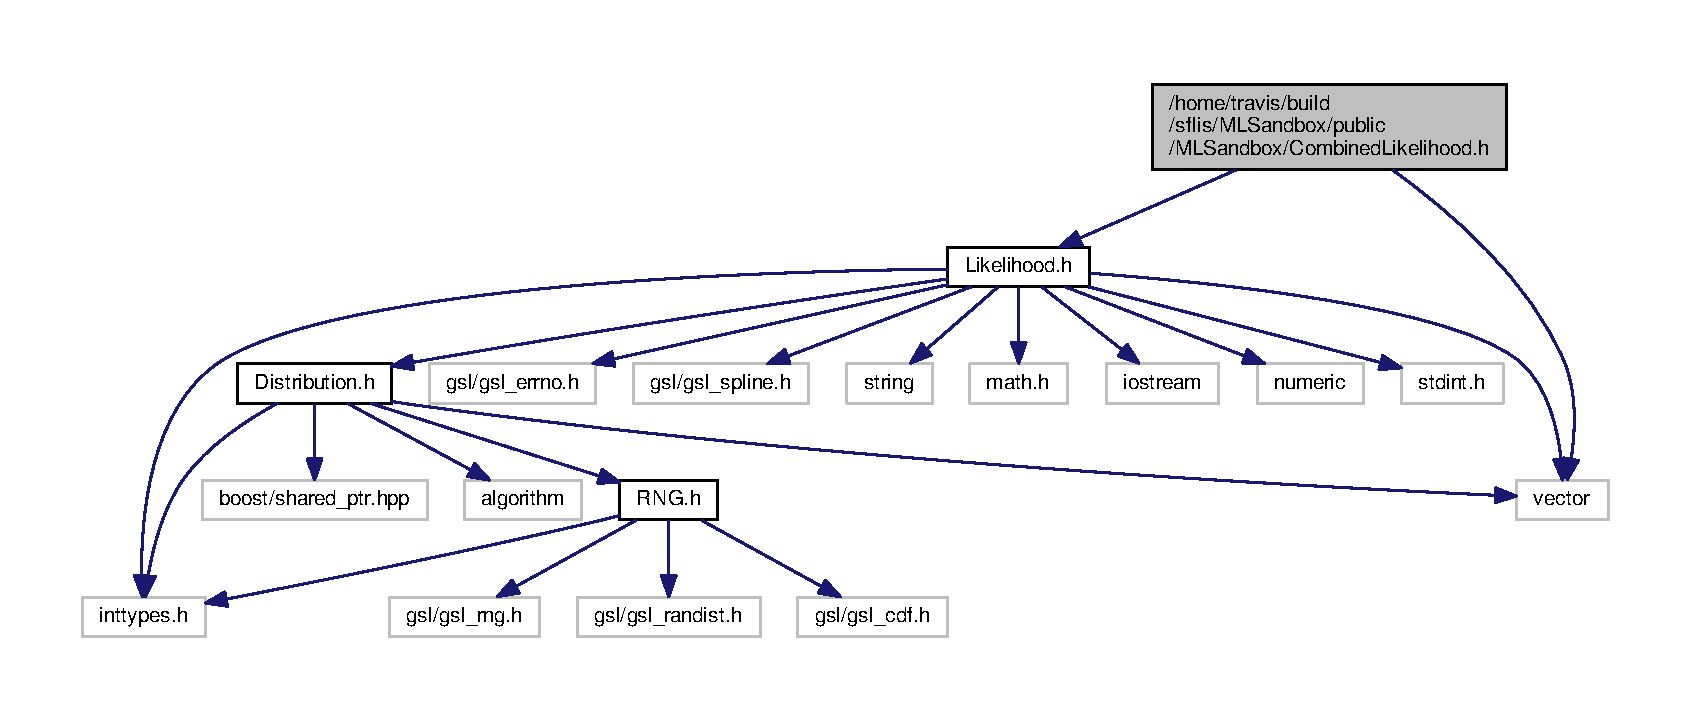
\includegraphics[width=350pt]{CombinedLikelihood_8h__incl}
\end{center}
\end{figure}
This graph shows which files directly or indirectly include this file\-:
\nopagebreak
\begin{figure}[H]
\begin{center}
\leavevmode
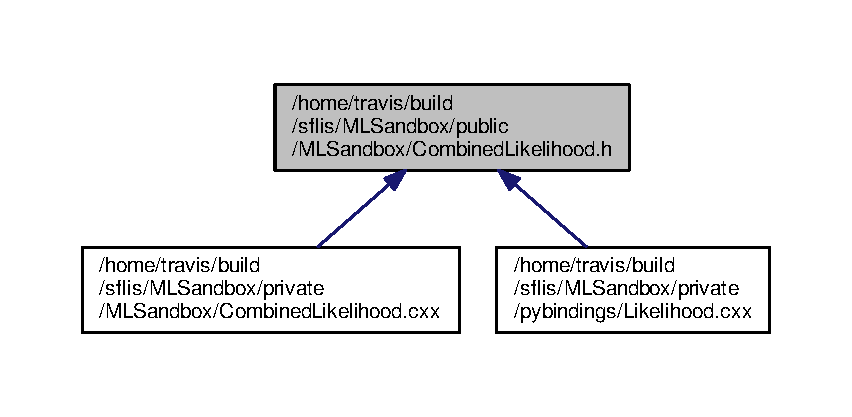
\includegraphics[width=350pt]{CombinedLikelihood_8h__dep__incl}
\end{center}
\end{figure}
\subsection*{Classes}
\begin{DoxyCompactItemize}
\item 
class \hyperlink{classCombinedLikelihood}{Combined\-Likelihood}
\end{DoxyCompactItemize}

\hypertarget{Distribution_8h}{\section{/home/travis/build/sflis/\-M\-L\-Sandbox/public/\-M\-L\-Sandbox/\-Distribution.h File Reference}
\label{Distribution_8h}\index{/home/travis/build/sflis/\-M\-L\-Sandbox/public/\-M\-L\-Sandbox/\-Distribution.\-h@{/home/travis/build/sflis/\-M\-L\-Sandbox/public/\-M\-L\-Sandbox/\-Distribution.\-h}}
}
{\ttfamily \#include $<$inttypes.\-h$>$}\\*
{\ttfamily \#include $<$vector$>$}\\*
{\ttfamily \#include $<$boost/shared\-\_\-ptr.\-hpp$>$}\\*
{\ttfamily \#include \char`\"{}R\-N\-G.\-h\char`\"{}}\\*
{\ttfamily \#include $<$algorithm$>$}\\*
Include dependency graph for Distribution.\-h\-:
\nopagebreak
\begin{figure}[H]
\begin{center}
\leavevmode
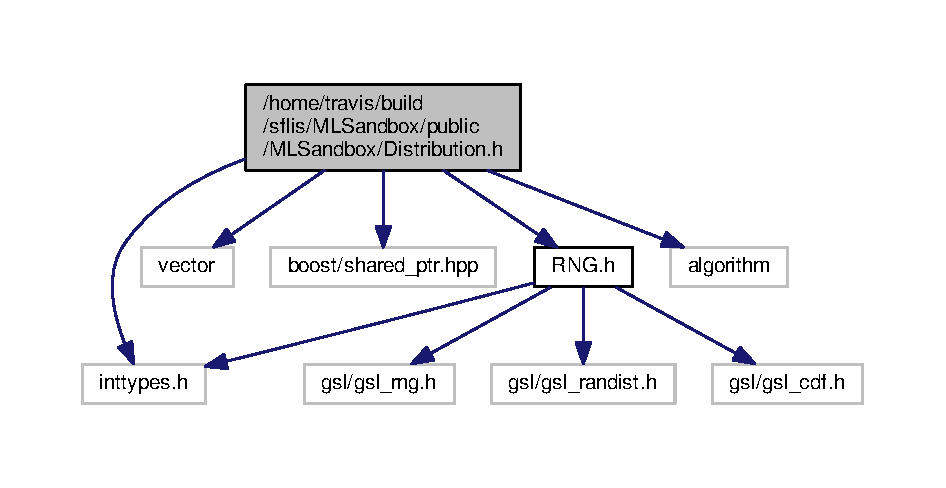
\includegraphics[width=350pt]{Distribution_8h__incl}
\end{center}
\end{figure}
This graph shows which files directly or indirectly include this file\-:
\nopagebreak
\begin{figure}[H]
\begin{center}
\leavevmode
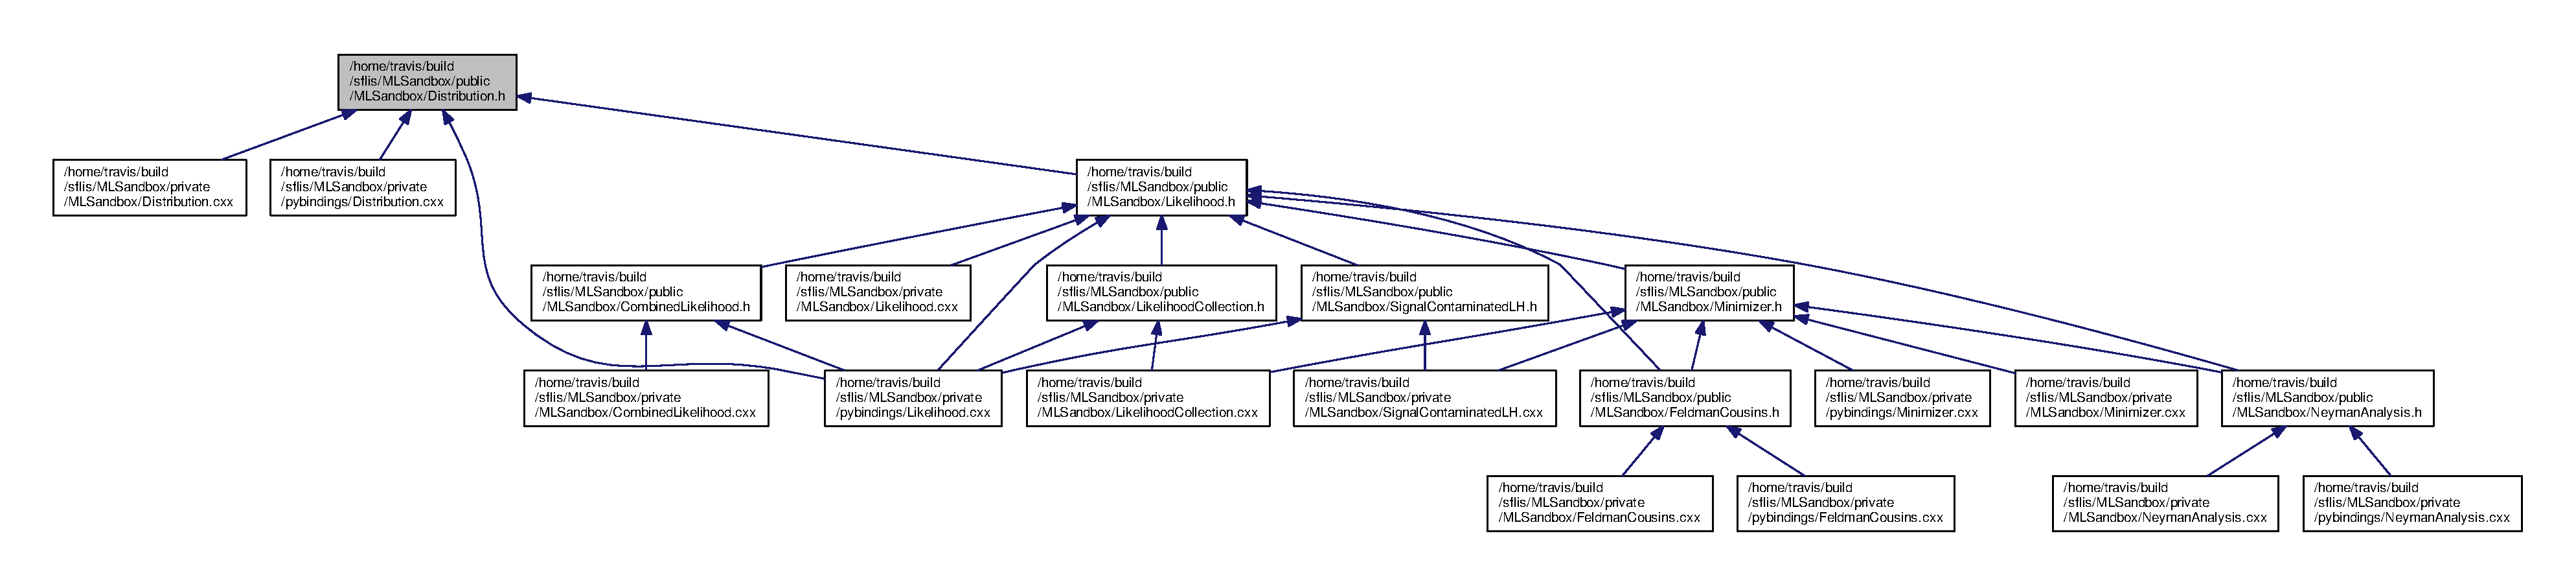
\includegraphics[width=350pt]{Distribution_8h__dep__incl}
\end{center}
\end{figure}
\subsection*{Classes}
\begin{DoxyCompactItemize}
\item 
class \hyperlink{classDistribution}{Distribution}
\begin{DoxyCompactList}\small\item\em A class that provides a common interface for binned distributions which are used to represent binned pdfs in likelihood objects. \end{DoxyCompactList}\end{DoxyCompactItemize}
\subsection*{Functions}
\begin{DoxyCompactItemize}
\item 
void \hyperlink{Distribution_8h_ab7b6b8c6018ab181645199038b0dba3a}{add\-Distributions} (double w1, \hyperlink{classDistribution}{Distribution} const \&dst1, double w2, \hyperlink{classDistribution}{Distribution} const \&dst2, \hyperlink{classDistribution}{Distribution} \&target)
\end{DoxyCompactItemize}


\subsection{Function Documentation}
\hypertarget{Distribution_8h_ab7b6b8c6018ab181645199038b0dba3a}{\index{Distribution.\-h@{Distribution.\-h}!add\-Distributions@{add\-Distributions}}
\index{add\-Distributions@{add\-Distributions}!Distribution.h@{Distribution.\-h}}
\subsubsection[{add\-Distributions}]{\setlength{\rightskip}{0pt plus 5cm}void add\-Distributions (
\begin{DoxyParamCaption}
\item[{double}]{w1, }
\item[{{\bf Distribution} const \&}]{dst1, }
\item[{double}]{w2, }
\item[{{\bf Distribution} const \&}]{dst2, }
\item[{{\bf Distribution} \&}]{target}
\end{DoxyParamCaption}
)\hspace{0.3cm}{\ttfamily [inline]}}}\label{Distribution_8h_ab7b6b8c6018ab181645199038b0dba3a}
A helper function that performs an addition operation on two distributions and putting the result in a third distribution object 
\hypertarget{FCRanks_8h}{\section{/home/travis/build/sflis/\-M\-L\-Sandbox/public/\-M\-L\-Sandbox/\-F\-C\-Ranks.h File Reference}
\label{FCRanks_8h}\index{/home/travis/build/sflis/\-M\-L\-Sandbox/public/\-M\-L\-Sandbox/\-F\-C\-Ranks.\-h@{/home/travis/build/sflis/\-M\-L\-Sandbox/public/\-M\-L\-Sandbox/\-F\-C\-Ranks.\-h}}
}
{\ttfamily \#include $<$boost/shared\-\_\-ptr.\-hpp$>$}\\*
{\ttfamily \#include $<$boost/serialization/vector.\-hpp$>$}\\*
{\ttfamily \#include $<$boost/serialization/map.\-hpp$>$}\\*
{\ttfamily \#include $<$boost/serialization/version.\-hpp$>$}\\*
{\ttfamily \#include $<$gsl/gsl\-\_\-errno.\-h$>$}\\*
{\ttfamily \#include $<$gsl/gsl\-\_\-spline.\-h$>$}\\*
{\ttfamily \#include $<$gsl/gsl\-\_\-cdf.\-h$>$}\\*
{\ttfamily \#include $<$inttypes.\-h$>$}\\*
{\ttfamily \#include $<$vector$>$}\\*
{\ttfamily \#include $<$map$>$}\\*
{\ttfamily \#include $<$string$>$}\\*
{\ttfamily \#include $<$iostream$>$}\\*
{\ttfamily \#include $<$algorithm$>$}\\*
Include dependency graph for F\-C\-Ranks.\-h\-:
\nopagebreak
\begin{figure}[H]
\begin{center}
\leavevmode
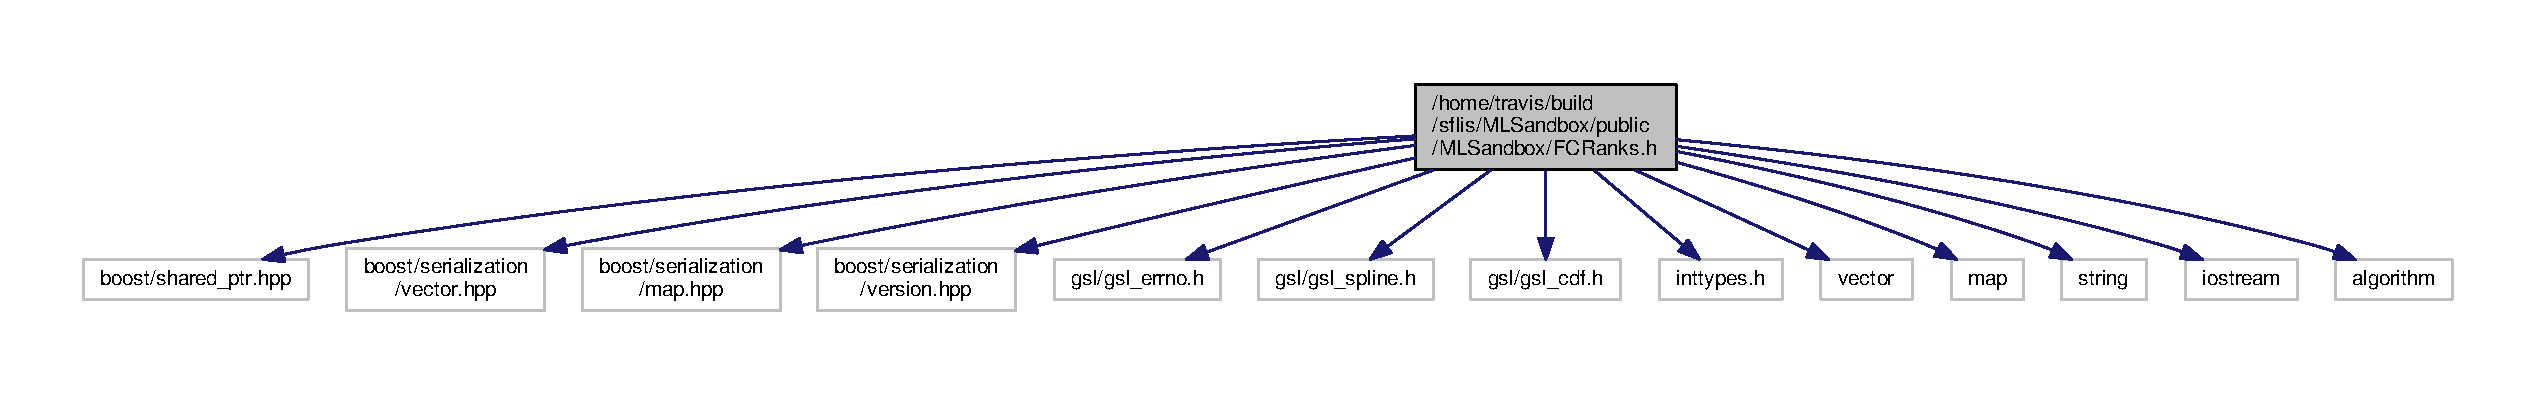
\includegraphics[width=350pt]{FCRanks_8h__incl}
\end{center}
\end{figure}
This graph shows which files directly or indirectly include this file\-:
\nopagebreak
\begin{figure}[H]
\begin{center}
\leavevmode
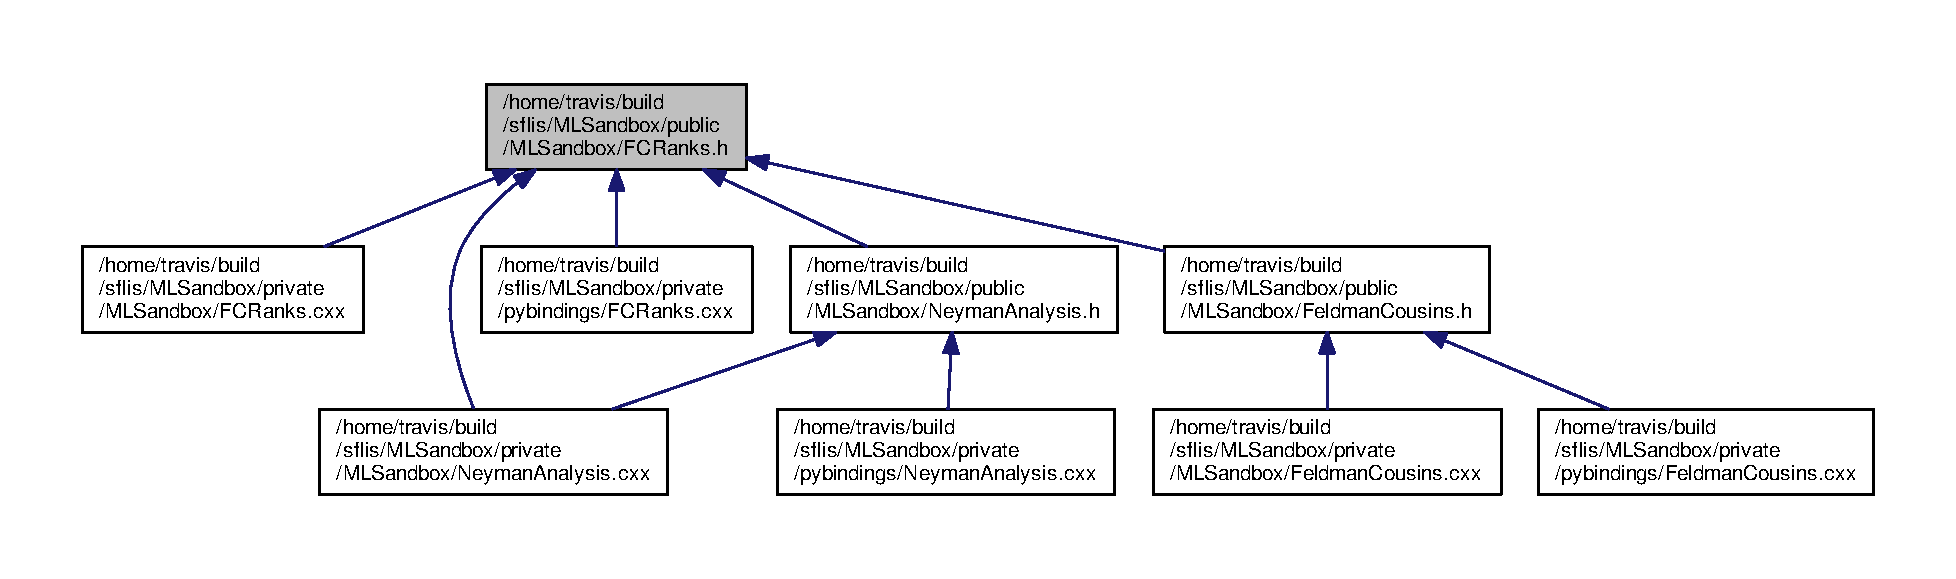
\includegraphics[width=350pt]{FCRanks_8h__dep__incl}
\end{center}
\end{figure}
\subsection*{Classes}
\begin{DoxyCompactItemize}
\item 
class \hyperlink{classFCRanks}{F\-C\-Ranks}
\begin{DoxyCompactList}\small\item\em A class that holds Feldman Cousins rank distribtions and provides some utilities to interpolate the critical boundary at different confidence levels. \end{DoxyCompactList}\end{DoxyCompactItemize}
\subsection*{Namespaces}
\begin{DoxyCompactItemize}
\item 
\hyperlink{namespacemlsandbox}{mlsandbox}
\end{DoxyCompactItemize}
\subsection*{Functions}
\begin{DoxyCompactItemize}
\item 
void \hyperlink{namespacemlsandbox_a8c015d48e7a9a7e3885263581f3e82cc}{mlsandbox\-::save\-F\-C\-Ranks} (std\-::string file\-\_\-name, \hyperlink{classFCRanks}{F\-C\-Ranks} \&ranks)
\item 
\hyperlink{classFCRanks}{F\-C\-Ranks} \hyperlink{namespacemlsandbox_a484593308083eeeff406c8baaa17447e}{mlsandbox\-::load\-F\-C\-Ranks} (std\-::string file\-\_\-name)
\end{DoxyCompactItemize}
\subsection*{Variables}
\begin{DoxyCompactItemize}
\item 
const unsigned int \hyperlink{FCRanks_8h_a8fabbafa59c3cb0a6834264e13831795}{F\-C\-R\-A\-N\-K\-S\-\_\-\-V\-E\-R\-S\-I\-O\-N} = 1
\end{DoxyCompactItemize}


\subsection{Variable Documentation}
\hypertarget{FCRanks_8h_a8fabbafa59c3cb0a6834264e13831795}{\index{F\-C\-Ranks.\-h@{F\-C\-Ranks.\-h}!F\-C\-R\-A\-N\-K\-S\-\_\-\-V\-E\-R\-S\-I\-O\-N@{F\-C\-R\-A\-N\-K\-S\-\_\-\-V\-E\-R\-S\-I\-O\-N}}
\index{F\-C\-R\-A\-N\-K\-S\-\_\-\-V\-E\-R\-S\-I\-O\-N@{F\-C\-R\-A\-N\-K\-S\-\_\-\-V\-E\-R\-S\-I\-O\-N}!FCRanks.h@{F\-C\-Ranks.\-h}}
\subsubsection[{F\-C\-R\-A\-N\-K\-S\-\_\-\-V\-E\-R\-S\-I\-O\-N}]{\setlength{\rightskip}{0pt plus 5cm}const unsigned int F\-C\-R\-A\-N\-K\-S\-\_\-\-V\-E\-R\-S\-I\-O\-N = 1}}\label{FCRanks_8h_a8fabbafa59c3cb0a6834264e13831795}

\hypertarget{FeldmanCousins_8h}{\section{/home/travis/build/sflis/\-M\-L\-Sandbox/public/\-M\-L\-Sandbox/\-Feldman\-Cousins.h File Reference}
\label{FeldmanCousins_8h}\index{/home/travis/build/sflis/\-M\-L\-Sandbox/public/\-M\-L\-Sandbox/\-Feldman\-Cousins.\-h@{/home/travis/build/sflis/\-M\-L\-Sandbox/public/\-M\-L\-Sandbox/\-Feldman\-Cousins.\-h}}
}
{\ttfamily \#include \char`\"{}Likelihood.\-h\char`\"{}}\\*
{\ttfamily \#include \char`\"{}Minimizer.\-h\char`\"{}}\\*
{\ttfamily \#include \char`\"{}F\-C\-Ranks.\-h\char`\"{}}\\*
{\ttfamily \#include $<$boost/shared\-\_\-ptr.\-hpp$>$}\\*
{\ttfamily \#include $<$gsl/gsl\-\_\-errno.\-h$>$}\\*
{\ttfamily \#include $<$gsl/gsl\-\_\-spline.\-h$>$}\\*
{\ttfamily \#include $<$inttypes.\-h$>$}\\*
{\ttfamily \#include $<$vector$>$}\\*
{\ttfamily \#include $<$string$>$}\\*
{\ttfamily \#include $<$math.\-h$>$}\\*
{\ttfamily \#include $<$iostream$>$}\\*
{\ttfamily \#include $<$boost/numpy.\-hpp$>$}\\*
Include dependency graph for Feldman\-Cousins.\-h\-:
\nopagebreak
\begin{figure}[H]
\begin{center}
\leavevmode
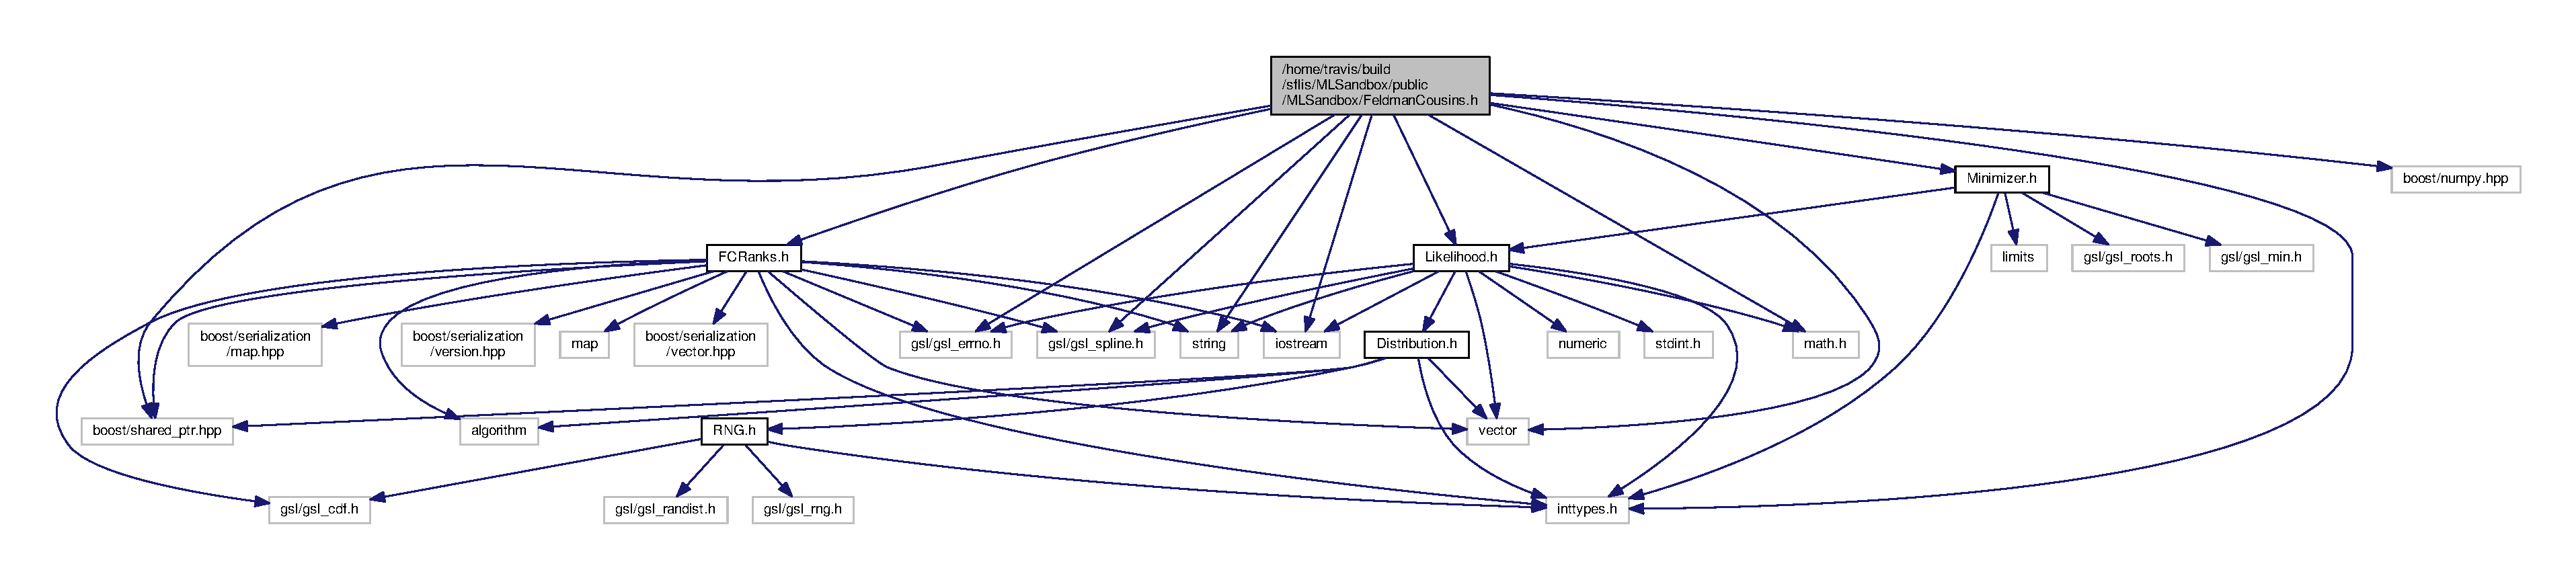
\includegraphics[width=350pt]{FeldmanCousins_8h__incl}
\end{center}
\end{figure}
This graph shows which files directly or indirectly include this file\-:
\nopagebreak
\begin{figure}[H]
\begin{center}
\leavevmode
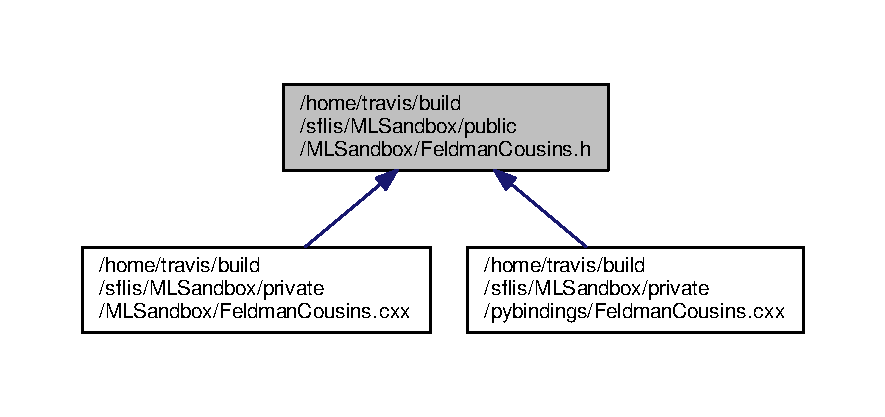
\includegraphics[width=350pt]{FeldmanCousins_8h__dep__incl}
\end{center}
\end{figure}
\subsection*{Classes}
\begin{DoxyCompactItemize}
\item 
class \hyperlink{classFeldmanCousinsAnalysis}{Feldman\-Cousins\-Analysis}
\end{DoxyCompactItemize}

\hypertarget{Likelihood_8h}{\section{/home/travis/build/sflis/\-M\-L\-Sandbox/public/\-M\-L\-Sandbox/\-Likelihood.h File Reference}
\label{Likelihood_8h}\index{/home/travis/build/sflis/\-M\-L\-Sandbox/public/\-M\-L\-Sandbox/\-Likelihood.\-h@{/home/travis/build/sflis/\-M\-L\-Sandbox/public/\-M\-L\-Sandbox/\-Likelihood.\-h}}
}
{\ttfamily \#include \char`\"{}Distribution.\-h\char`\"{}}\\*
{\ttfamily \#include $<$gsl/gsl\-\_\-errno.\-h$>$}\\*
{\ttfamily \#include $<$gsl/gsl\-\_\-spline.\-h$>$}\\*
{\ttfamily \#include $<$inttypes.\-h$>$}\\*
{\ttfamily \#include $<$vector$>$}\\*
{\ttfamily \#include $<$string$>$}\\*
{\ttfamily \#include $<$math.\-h$>$}\\*
{\ttfamily \#include $<$iostream$>$}\\*
{\ttfamily \#include $<$numeric$>$}\\*
{\ttfamily \#include \char`\"{}stdint.\-h\char`\"{}}\\*
Include dependency graph for Likelihood.\-h\-:
\nopagebreak
\begin{figure}[H]
\begin{center}
\leavevmode
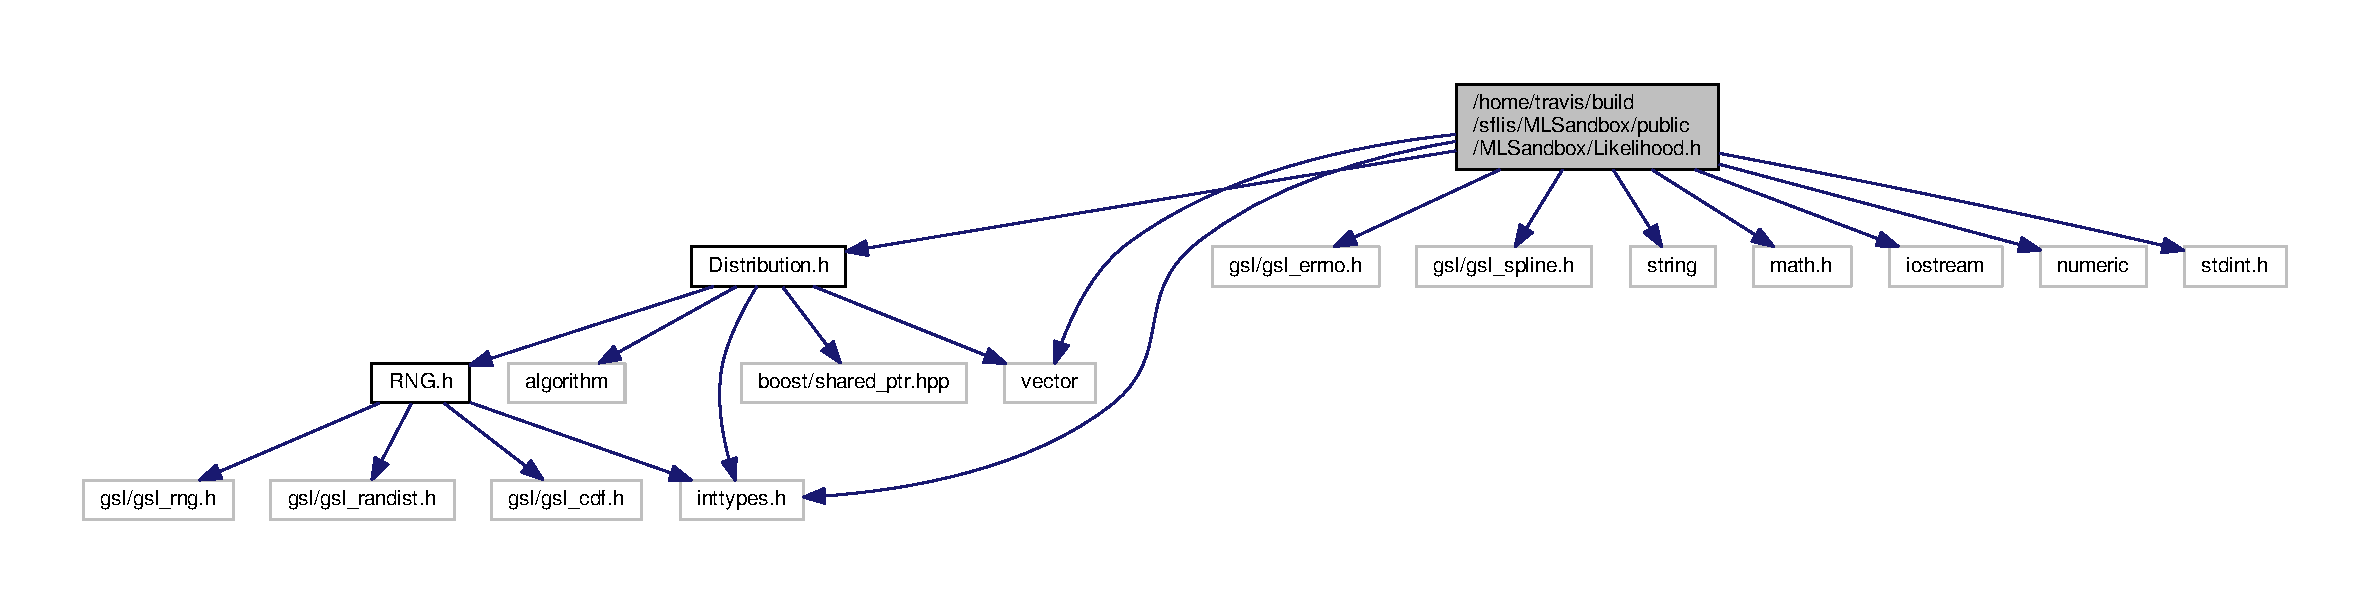
\includegraphics[width=350pt]{Likelihood_8h__incl}
\end{center}
\end{figure}
This graph shows which files directly or indirectly include this file\-:
\nopagebreak
\begin{figure}[H]
\begin{center}
\leavevmode
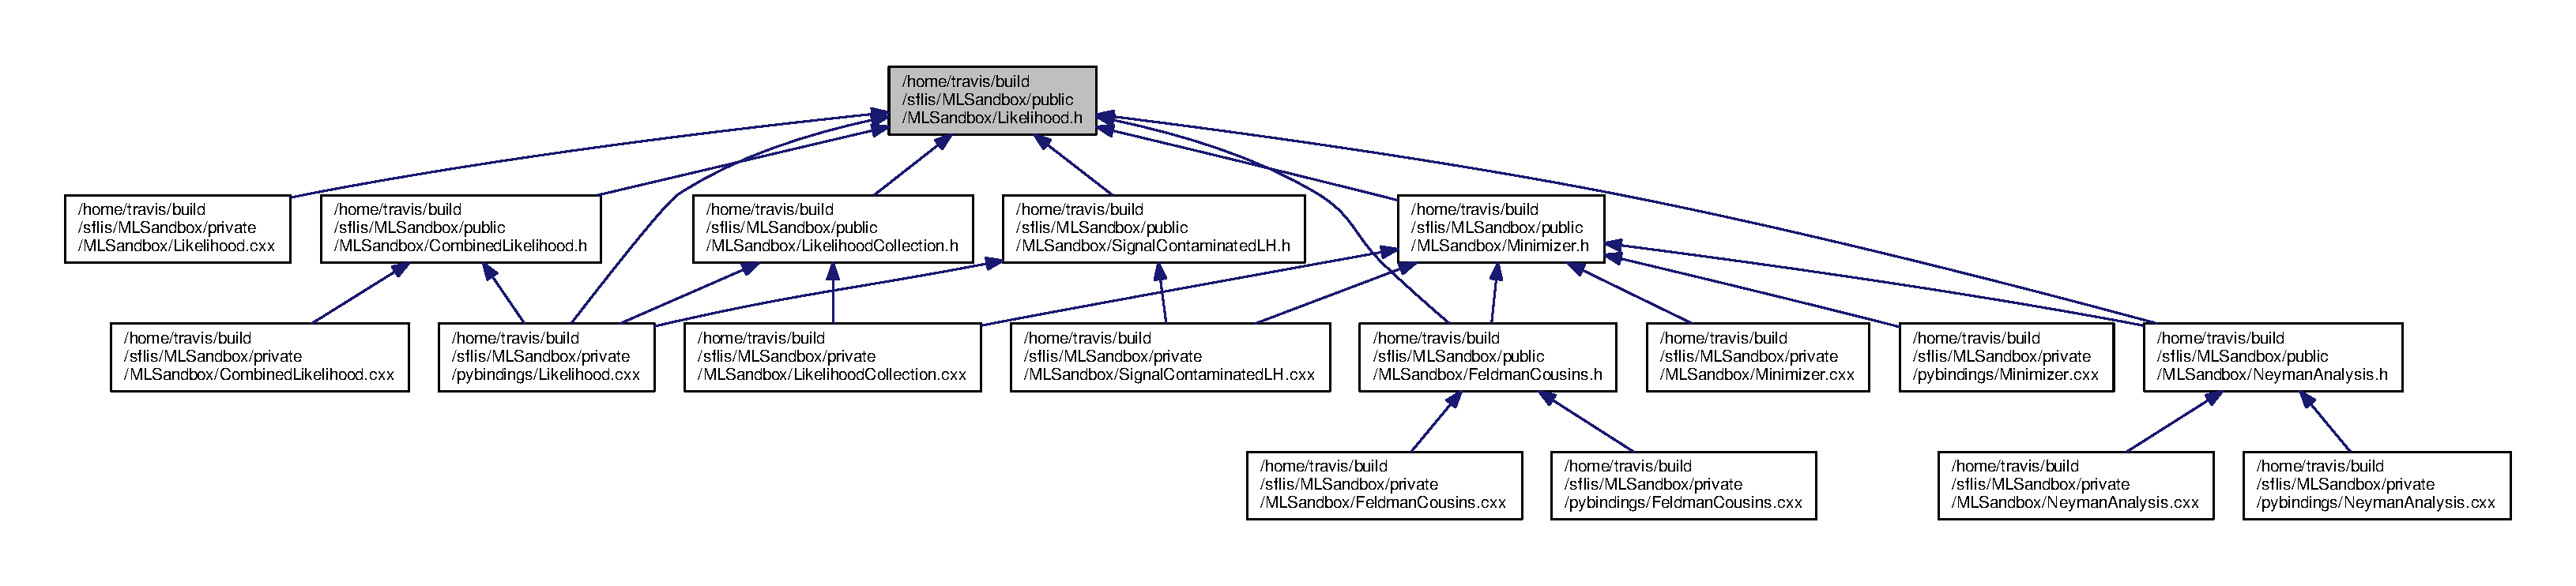
\includegraphics[width=350pt]{Likelihood_8h__dep__incl}
\end{center}
\end{figure}
\subsection*{Classes}
\begin{DoxyCompactItemize}
\item 
class \hyperlink{classLikelihood}{Likelihood}
\begin{DoxyCompactList}\small\item\em A base class (wrapper class) for likelihoods which defines a general interface needed analysis classes. \end{DoxyCompactList}\item 
class \hyperlink{classBinnedLikelihood}{Binned\-Likelihood}
\item 
class \hyperlink{classShapeLikelihood}{Shape\-Likelihood}
\begin{DoxyCompactList}\small\item\em A class that provides functions to compute a 1 dimensional \hyperlink{classLikelihood}{Likelihood} of the form\-: \[ L(\xi) = \prod^N_{k=1} (\xi f_{sig}(x_k) + (1-\xi) f_{bg}(x_k)) \]. \end{DoxyCompactList}\end{DoxyCompactItemize}
\subsection*{Macros}
\begin{DoxyCompactItemize}
\item 
\#define \hyperlink{Likelihood_8h_abc7d71657be8975a51684e41029b7964}{get16bits}(d)
\end{DoxyCompactItemize}
\subsection*{Typedefs}
\begin{DoxyCompactItemize}
\item 
typedef double($\ast$ \hyperlink{Likelihood_8h_a97d92c5c141f28319e7e8198defc9084}{likelihood\-Callback} )(double, void $\ast$)
\end{DoxyCompactItemize}
\subsection*{Functions}
\begin{DoxyCompactItemize}
\item 
uint32\-\_\-t \hyperlink{Likelihood_8h_a11d69a8cb5ac90dfb13d2e25df8eb1ce}{Super\-Fast\-Hash} (const char $\ast$data, int len)
\end{DoxyCompactItemize}


\subsection{Macro Definition Documentation}
\hypertarget{Likelihood_8h_abc7d71657be8975a51684e41029b7964}{\index{Likelihood.\-h@{Likelihood.\-h}!get16bits@{get16bits}}
\index{get16bits@{get16bits}!Likelihood.h@{Likelihood.\-h}}
\subsubsection[{get16bits}]{\setlength{\rightskip}{0pt plus 5cm}\#define get16bits(
\begin{DoxyParamCaption}
\item[{}]{d}
\end{DoxyParamCaption}
)}}\label{Likelihood_8h_abc7d71657be8975a51684e41029b7964}
{\bfseries Value\-:}
\begin{DoxyCode}
((((uint32\_t)(((\textcolor{keyword}{const} uint8\_t *)(d))[1])) << 8)\(\backslash\)
                       +(uint32\_t)(((\textcolor{keyword}{const} uint8\_t *)(d))[0]) )
\end{DoxyCode}


\subsection{Typedef Documentation}
\hypertarget{Likelihood_8h_a97d92c5c141f28319e7e8198defc9084}{\index{Likelihood.\-h@{Likelihood.\-h}!likelihood\-Callback@{likelihood\-Callback}}
\index{likelihood\-Callback@{likelihood\-Callback}!Likelihood.h@{Likelihood.\-h}}
\subsubsection[{likelihood\-Callback}]{\setlength{\rightskip}{0pt plus 5cm}typedef double($\ast$ likelihood\-Callback)(double, void $\ast$)}}\label{Likelihood_8h_a97d92c5c141f28319e7e8198defc9084}


\subsection{Function Documentation}
\hypertarget{Likelihood_8h_a11d69a8cb5ac90dfb13d2e25df8eb1ce}{\index{Likelihood.\-h@{Likelihood.\-h}!Super\-Fast\-Hash@{Super\-Fast\-Hash}}
\index{Super\-Fast\-Hash@{Super\-Fast\-Hash}!Likelihood.h@{Likelihood.\-h}}
\subsubsection[{Super\-Fast\-Hash}]{\setlength{\rightskip}{0pt plus 5cm}uint32\-\_\-t Super\-Fast\-Hash (
\begin{DoxyParamCaption}
\item[{const char $\ast$}]{data, }
\item[{int}]{len}
\end{DoxyParamCaption}
)}}\label{Likelihood_8h_a11d69a8cb5ac90dfb13d2e25df8eb1ce}

\hypertarget{LikelihoodCollection_8h}{\section{/home/travis/build/sflis/\-M\-L\-Sandbox/public/\-M\-L\-Sandbox/\-Likelihood\-Collection.h File Reference}
\label{LikelihoodCollection_8h}\index{/home/travis/build/sflis/\-M\-L\-Sandbox/public/\-M\-L\-Sandbox/\-Likelihood\-Collection.\-h@{/home/travis/build/sflis/\-M\-L\-Sandbox/public/\-M\-L\-Sandbox/\-Likelihood\-Collection.\-h}}
}
{\ttfamily \#include \char`\"{}M\-L\-Sandbox/\-Likelihood.\-h\char`\"{}}\\*
{\ttfamily \#include $<$iostream$>$}\\*
{\ttfamily \#include $<$string$>$}\\*
{\ttfamily \#include $<$map$>$}\\*
Include dependency graph for Likelihood\-Collection.\-h\-:
\nopagebreak
\begin{figure}[H]
\begin{center}
\leavevmode
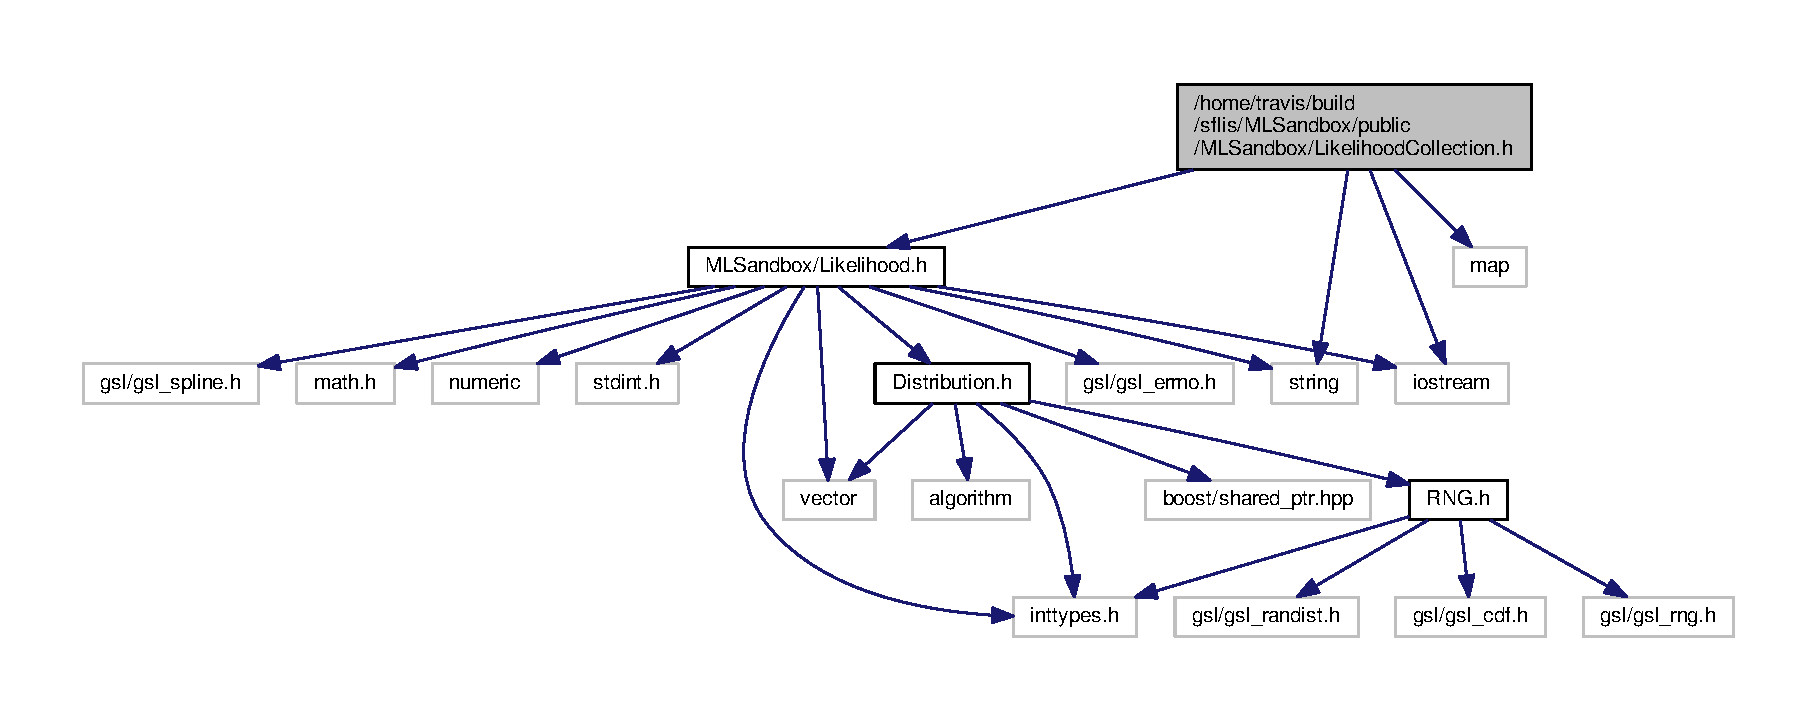
\includegraphics[width=350pt]{LikelihoodCollection_8h__incl}
\end{center}
\end{figure}
This graph shows which files directly or indirectly include this file\-:
\nopagebreak
\begin{figure}[H]
\begin{center}
\leavevmode
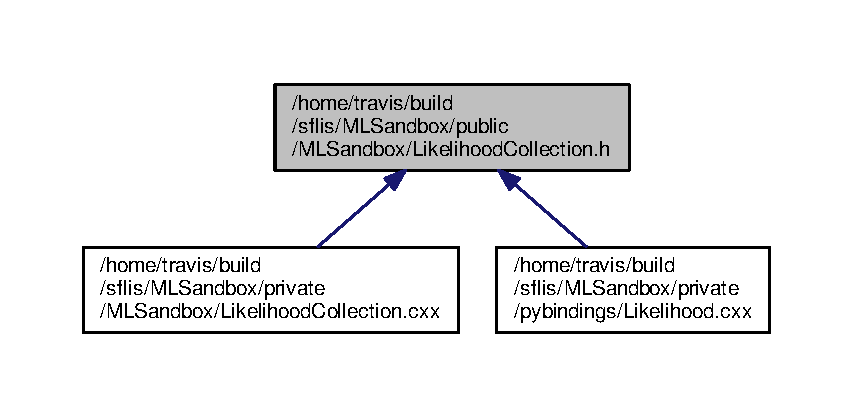
\includegraphics[width=350pt]{LikelihoodCollection_8h__dep__incl}
\end{center}
\end{figure}
\subsection*{Classes}
\begin{DoxyCompactItemize}
\item 
class \hyperlink{classLikelihoodCollection}{Likelihood\-Collection}
\end{DoxyCompactItemize}

\hypertarget{Minimizer_8h}{\section{/home/travis/build/sflis/\-M\-L\-Sandbox/public/\-M\-L\-Sandbox/\-Minimizer.h File Reference}
\label{Minimizer_8h}\index{/home/travis/build/sflis/\-M\-L\-Sandbox/public/\-M\-L\-Sandbox/\-Minimizer.\-h@{/home/travis/build/sflis/\-M\-L\-Sandbox/public/\-M\-L\-Sandbox/\-Minimizer.\-h}}
}
{\ttfamily \#include $<$inttypes.\-h$>$}\\*
{\ttfamily \#include $<$gsl/gsl\-\_\-roots.\-h$>$}\\*
{\ttfamily \#include $<$gsl/gsl\-\_\-min.\-h$>$}\\*
{\ttfamily \#include $<$limits$>$}\\*
{\ttfamily \#include \char`\"{}Likelihood.\-h\char`\"{}}\\*
Include dependency graph for Minimizer.\-h\-:
\nopagebreak
\begin{figure}[H]
\begin{center}
\leavevmode
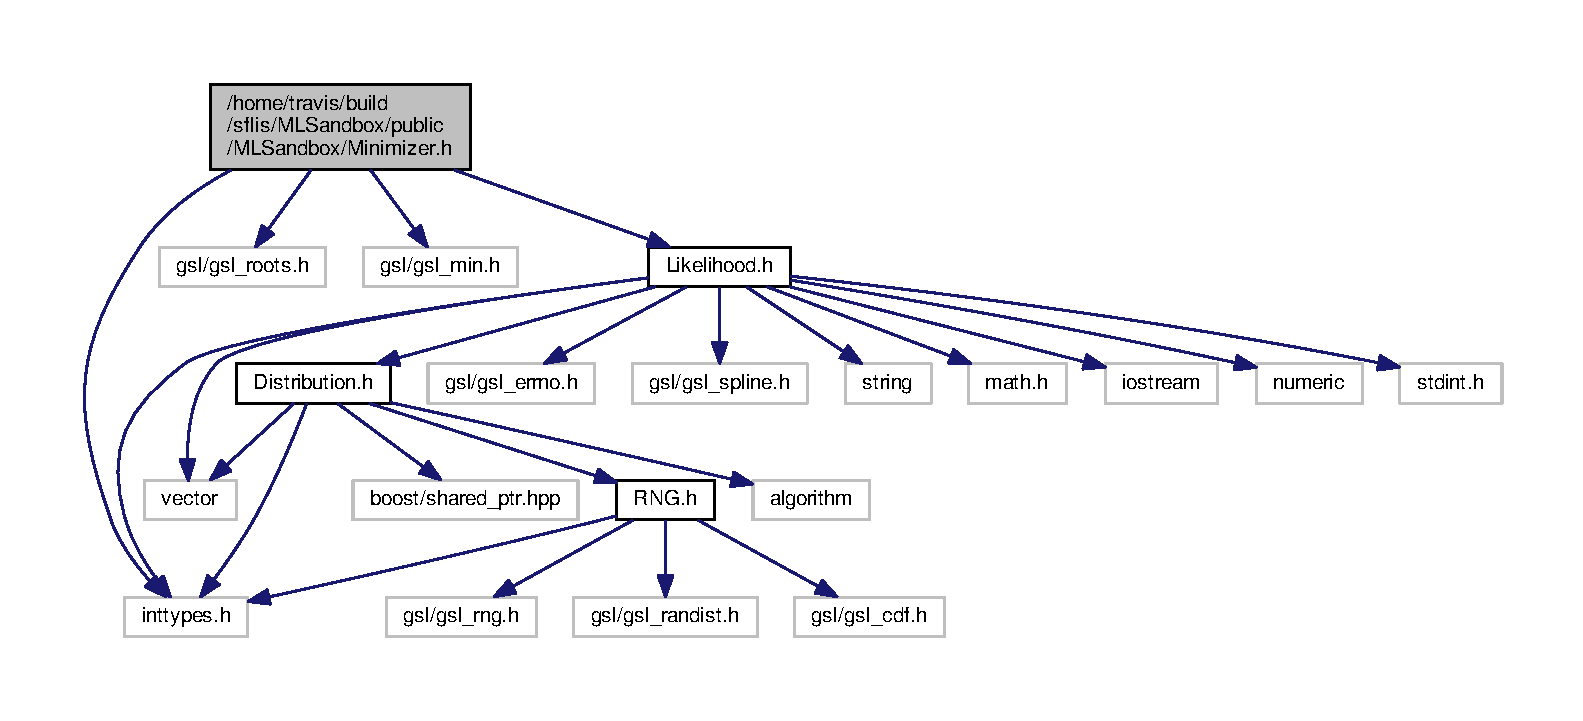
\includegraphics[width=350pt]{Minimizer_8h__incl}
\end{center}
\end{figure}
This graph shows which files directly or indirectly include this file\-:
\nopagebreak
\begin{figure}[H]
\begin{center}
\leavevmode
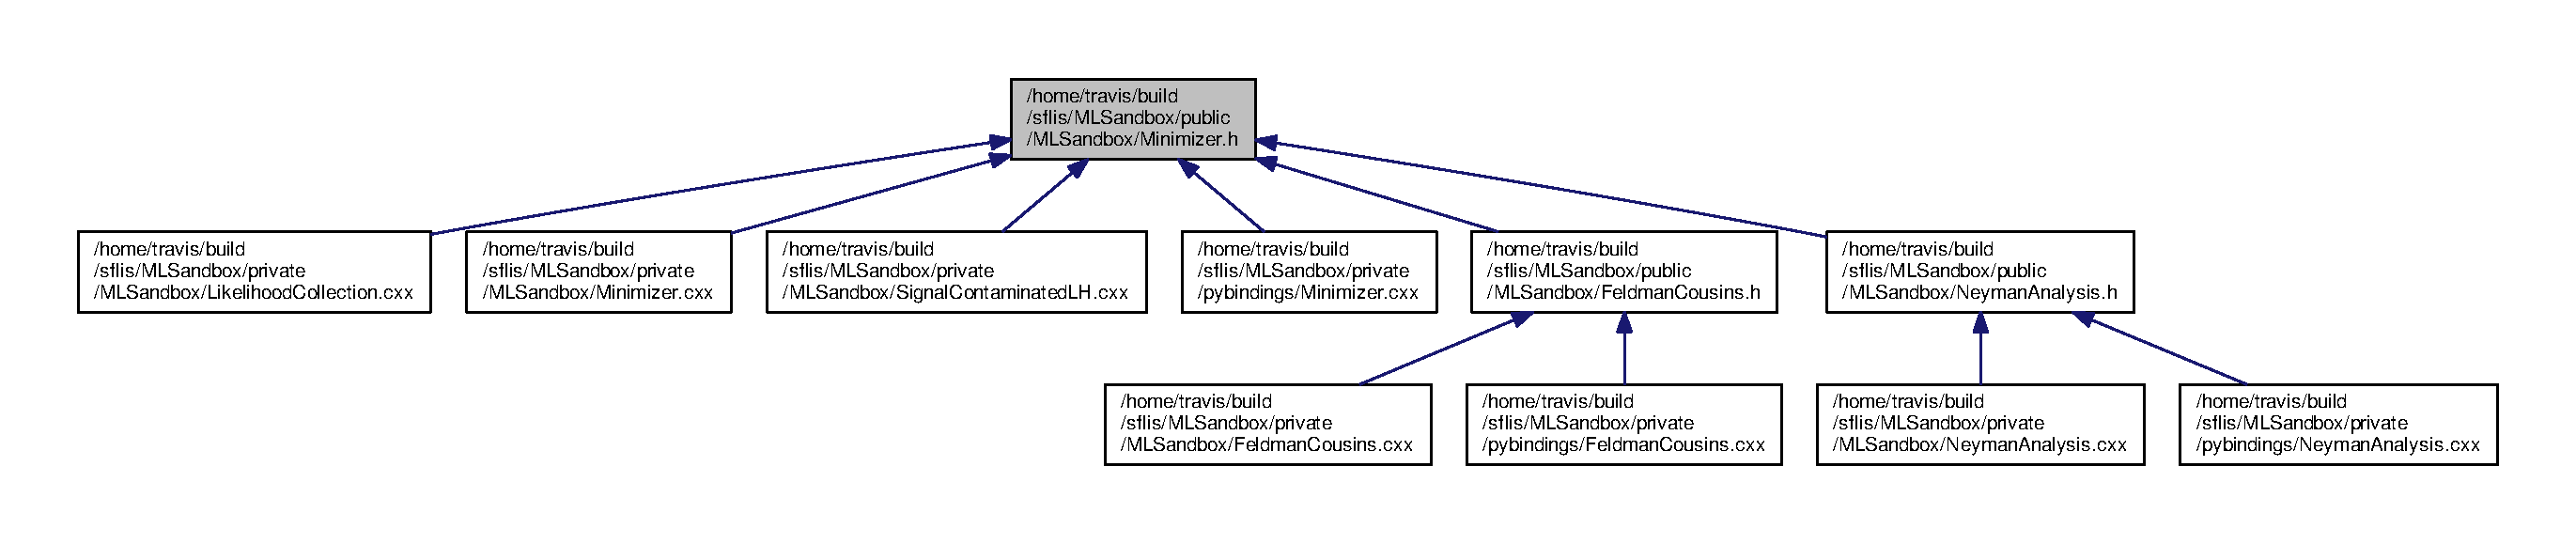
\includegraphics[width=350pt]{Minimizer_8h__dep__incl}
\end{center}
\end{figure}
\subsection*{Classes}
\begin{DoxyCompactItemize}
\item 
class \hyperlink{classMinimizer}{Minimizer}
\begin{DoxyCompactList}\small\item\em A small wrapper class around the G\-S\-L minimizer. \end{DoxyCompactList}\end{DoxyCompactItemize}

\hypertarget{NeymanAnalysis_8h}{\section{/home/travis/build/sflis/\-M\-L\-Sandbox/public/\-M\-L\-Sandbox/\-Neyman\-Analysis.h File Reference}
\label{NeymanAnalysis_8h}\index{/home/travis/build/sflis/\-M\-L\-Sandbox/public/\-M\-L\-Sandbox/\-Neyman\-Analysis.\-h@{/home/travis/build/sflis/\-M\-L\-Sandbox/public/\-M\-L\-Sandbox/\-Neyman\-Analysis.\-h}}
}
{\ttfamily \#include \char`\"{}Likelihood.\-h\char`\"{}}\\*
{\ttfamily \#include \char`\"{}Minimizer.\-h\char`\"{}}\\*
{\ttfamily \#include \char`\"{}F\-C\-Ranks.\-h\char`\"{}}\\*
{\ttfamily \#include $<$boost/shared\-\_\-ptr.\-hpp$>$}\\*
{\ttfamily \#include $<$gsl/gsl\-\_\-errno.\-h$>$}\\*
{\ttfamily \#include $<$gsl/gsl\-\_\-spline.\-h$>$}\\*
{\ttfamily \#include $<$inttypes.\-h$>$}\\*
{\ttfamily \#include $<$vector$>$}\\*
{\ttfamily \#include $<$string$>$}\\*
{\ttfamily \#include $<$math.\-h$>$}\\*
{\ttfamily \#include $<$iostream$>$}\\*
Include dependency graph for Neyman\-Analysis.\-h\-:
\nopagebreak
\begin{figure}[H]
\begin{center}
\leavevmode
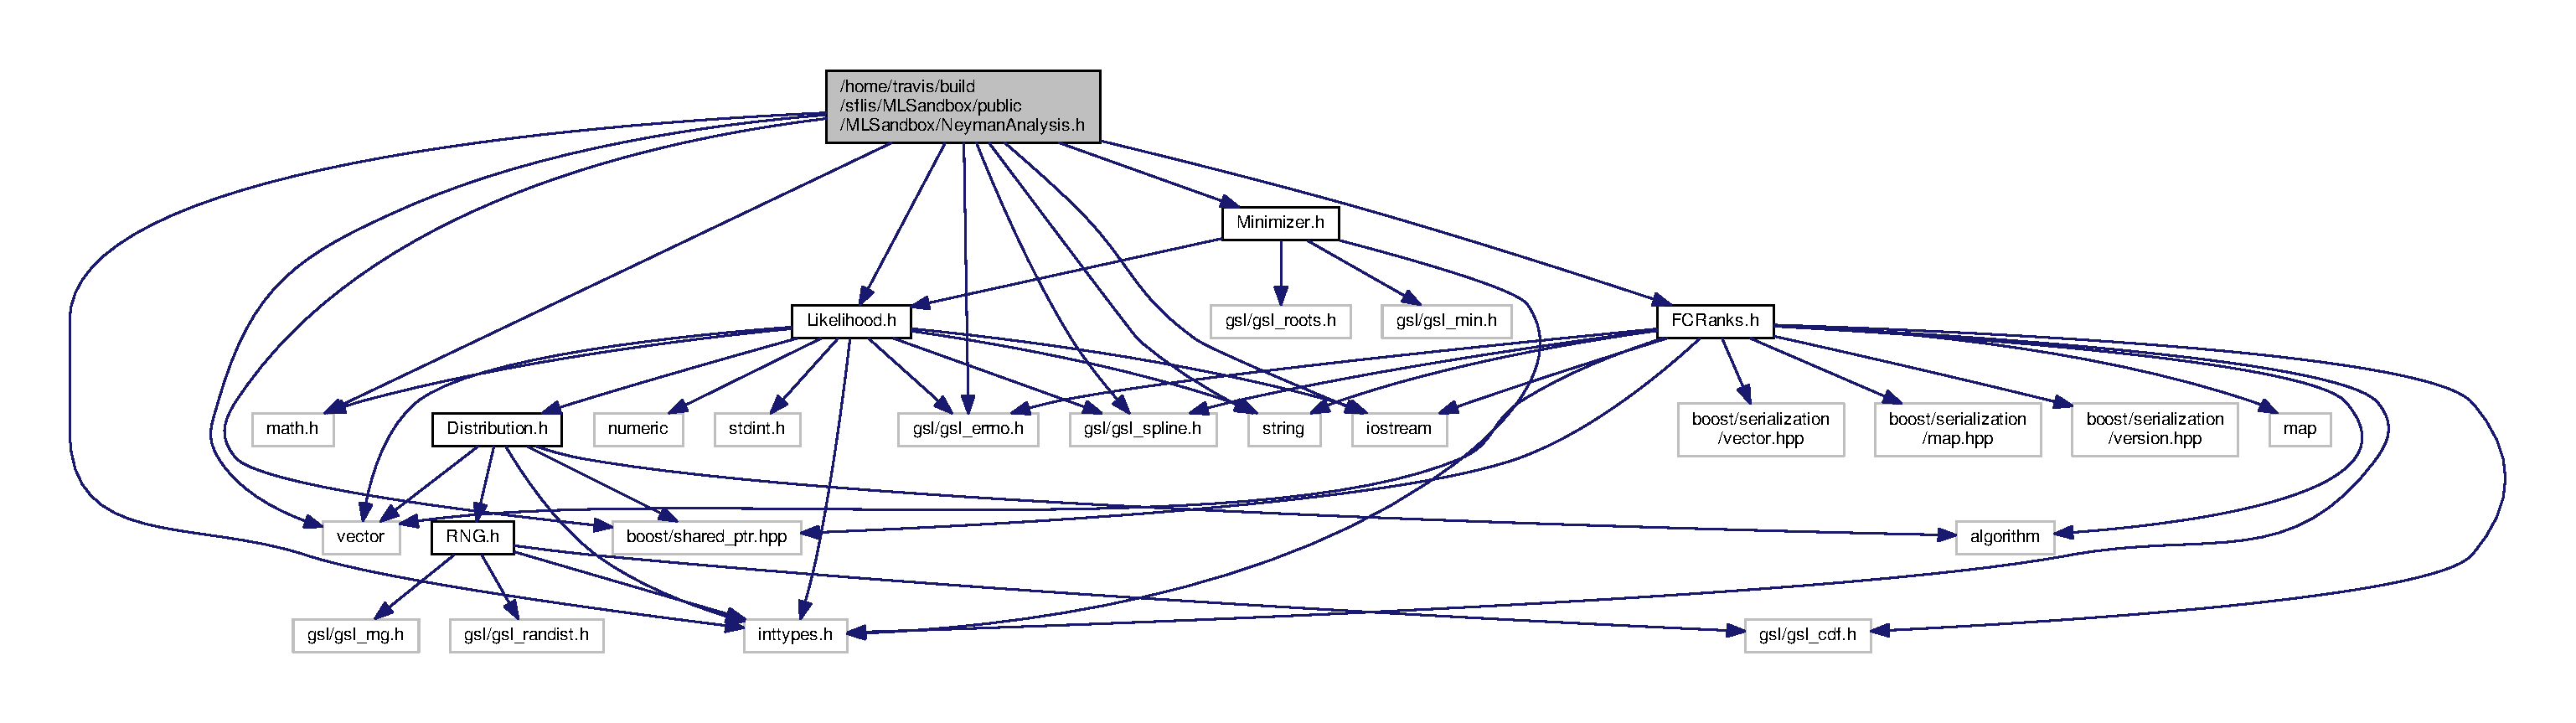
\includegraphics[width=350pt]{NeymanAnalysis_8h__incl}
\end{center}
\end{figure}
This graph shows which files directly or indirectly include this file\-:
\nopagebreak
\begin{figure}[H]
\begin{center}
\leavevmode
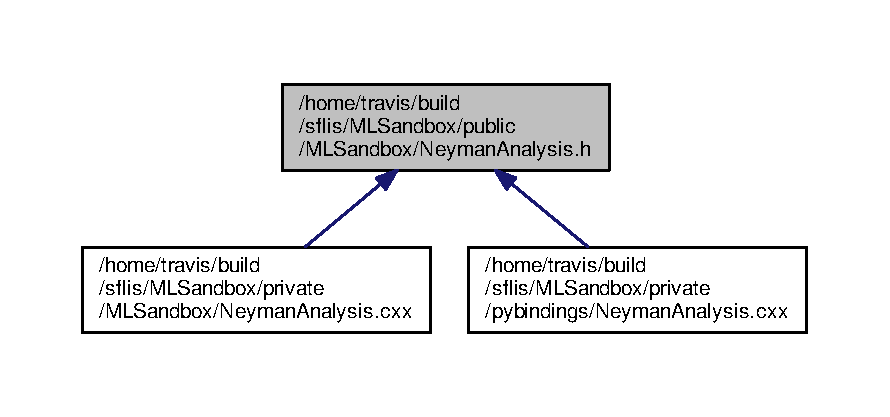
\includegraphics[width=350pt]{NeymanAnalysis_8h__dep__incl}
\end{center}
\end{figure}
\subsection*{Classes}
\begin{DoxyCompactItemize}
\item 
class \hyperlink{classNeymanAnalysis}{Neyman\-Analysis}
\end{DoxyCompactItemize}

\hypertarget{RNG_8h}{\section{/home/travis/build/sflis/\-M\-L\-Sandbox/public/\-M\-L\-Sandbox/\-R\-N\-G.h File Reference}
\label{RNG_8h}\index{/home/travis/build/sflis/\-M\-L\-Sandbox/public/\-M\-L\-Sandbox/\-R\-N\-G.\-h@{/home/travis/build/sflis/\-M\-L\-Sandbox/public/\-M\-L\-Sandbox/\-R\-N\-G.\-h}}
}
{\ttfamily \#include $<$inttypes.\-h$>$}\\*
{\ttfamily \#include $<$gsl/gsl\-\_\-rng.\-h$>$}\\*
{\ttfamily \#include $<$gsl/gsl\-\_\-randist.\-h$>$}\\*
{\ttfamily \#include $<$gsl/gsl\-\_\-cdf.\-h$>$}\\*
Include dependency graph for R\-N\-G.\-h\-:
\nopagebreak
\begin{figure}[H]
\begin{center}
\leavevmode
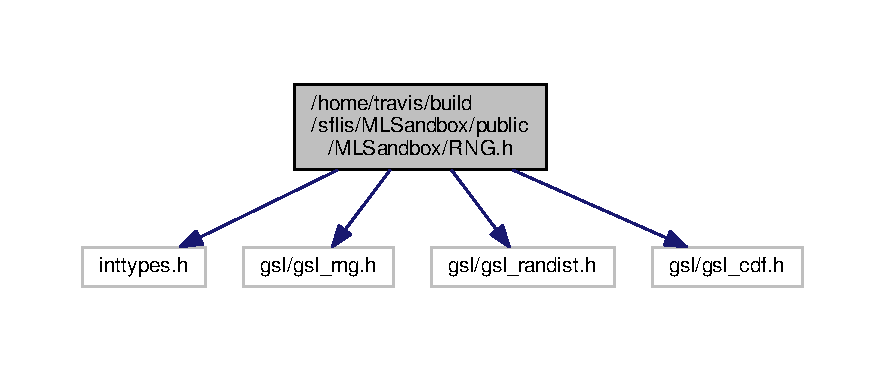
\includegraphics[width=350pt]{RNG_8h__incl}
\end{center}
\end{figure}
This graph shows which files directly or indirectly include this file\-:
\nopagebreak
\begin{figure}[H]
\begin{center}
\leavevmode
\includegraphics[width=350pt]{RNG_8h__dep__incl}
\end{center}
\end{figure}
\subsection*{Classes}
\begin{DoxyCompactItemize}
\item 
class \hyperlink{classRNG}{R\-N\-G}
\begin{DoxyCompactList}\small\item\em A small wrapper class around the G\-S\-L random number generator. \end{DoxyCompactList}\end{DoxyCompactItemize}

\hypertarget{SignalContaminatedLH_8h}{\section{/home/travis/build/sflis/\-M\-L\-Sandbox/public/\-M\-L\-Sandbox/\-Signal\-Contaminated\-L\-H.h File Reference}
\label{SignalContaminatedLH_8h}\index{/home/travis/build/sflis/\-M\-L\-Sandbox/public/\-M\-L\-Sandbox/\-Signal\-Contaminated\-L\-H.\-h@{/home/travis/build/sflis/\-M\-L\-Sandbox/public/\-M\-L\-Sandbox/\-Signal\-Contaminated\-L\-H.\-h}}
}
{\ttfamily \#include \char`\"{}M\-L\-Sandbox/\-Likelihood.\-h\char`\"{}}\\*
{\ttfamily \#include $<$iostream$>$}\\*
Include dependency graph for Signal\-Contaminated\-L\-H.\-h\-:
\nopagebreak
\begin{figure}[H]
\begin{center}
\leavevmode
\includegraphics[width=350pt]{SignalContaminatedLH_8h__incl}
\end{center}
\end{figure}
This graph shows which files directly or indirectly include this file\-:
\nopagebreak
\begin{figure}[H]
\begin{center}
\leavevmode
\includegraphics[width=350pt]{SignalContaminatedLH_8h__dep__incl}
\end{center}
\end{figure}
\subsection*{Classes}
\begin{DoxyCompactItemize}
\item 
class \hyperlink{classSignalContaminatedLH}{Signal\-Contaminated\-L\-H}
\end{DoxyCompactItemize}

%--- End generated contents ---

% Index
\newpage
\phantomsection
\addcontentsline{toc}{chapter}{Index}
\printindex

\end{document}
